\documentclass[12pt,letterpaper]{report}

\usepackage{sisl-suthesis}
\addbibresource{references}
\usepackage{amssymb}
\usepackage{amsthm}
\usepackage{graphicx}
\usepackage{subcaption} 
\usepackage{epigraph}
\usepackage[toc,page]{appendix}

\newtheorem{thm}{Theorem}[section]
\newtheorem{theorem}{Theorem}
\newtheorem{lem}[thm]{Lemma}
\newtheorem{corollary}{Corollary}
\newtheorem{prop}[theorem]{Proposition}
\newenvironment{sketch}{%
  \renewcommand{\proofname}{Proof Sketch}\proof}{\endproof}

\usepackage{hyperref}
\hypersetup{colorlinks,
%citecolor=blue
}

%% Thesis Metadata
\dept{Computer Science}

\title{Extensions and Applications of Deep Probabilistic \\ Inference for Generative Models}
\author{Mike Hongfei Wu}

% adviser and readers
\principaladviser{Noah Goodman}
\firstreader{Stefano Ermon}
\secondreader{Chelsea Finn}

\begin{document}

\beforepreface

\prefacesection{Abstract}
Despite the growth of data size, many applications for which we would like to apply learning algorithms are limited by data quantity and quality. Generative models propose a framework to naturally combine prior beliefs with real world data. Core to the generative approach is the challenge of probabilistic inference, or estimating latent variables given observations. This challenge has led to a rich field of research spanning many classes of statistical techniques. More recently, deep learning methods have been re-tooled to solve inference queries, aptly named \textit{deep inference}. In my dissertion I will explore algorithmic extensions to deep inference in response to real world challenges of sparsity and efficiency. I will present case studies of practical applications where deep inference achieves considerable improvements upon prior work.

This dissertation is centered around three parts. We  present the background for generative models and deep inference with an emphasis on modern variational methods. The first part will present new algorithms for generalizing inference to be robust to different notions of sparsity, such as multimodal data, missing data, or computational constraints. Second, we study \textit{meta}-amortized inference, or ``inferring how to infer''. A doubly-amortized inference algorithm would be cheaply able to solve inference queries for a novel generative model. We will show a new algorithm to re-purpose masked language modeling to do just this.

Third, we present three real-world applications of deep inference for: (a) estimating student abilities under item response theory and related psychometric models, (b) unsupervised feedback for student solutions to programming questions, and (c) compression of high resolution satellite imagery. Together, these contributions showcase the richness and utility of deep inference in the real world.

\prefacesection{Acknowledgments}
First of all, I would like to thank my PhD advisor, Noah Goodman. When I was choosing which graduate school to attend, one of my mentors said something along the lines of ``Go find Noah Goodman. He is a genius.''. Over five years, I have gotten to learn and re-learn what being a genius means. Noah's mentorship and guidance has been the principle component of what made my learning and my contributions possible. Thank you for teaching me how to be curious and how to search for the answers no matter how complex the problem. These are lessons that that I will take with me for many years to come.

The previous and current members of the ``CoCoLab'' have been indispensible collaborators and friends. Judy Fan and Robert Hawkins were early role models for me: two shining examples of what being stellar researchers is like; Ben Peloquin and Sahil Chopra were partners in crime. Thank you for helping me grow as a researcher and for all the fun we had along the way (I think back to those days we played basketball together with fond memories). As I slowly became a more senior student in CoCoLab, I had the priviledge of meeting more talented researchers. Alex Tamkin, Jesse Mu, and Rose Wang inspire me with their research vision and process. A special thank you to Rose for instilling new research drive in me in my final year. Outside of CoCoLab, Kristy Choi, Shyamal Buch, and Ali Malik have been pillars of my personal community at Stanford. Thank you for spending time with me. Whether it was tennis, meals, or talking shop, your friendships have enriched me academically and beyond.

I am greatly in debt to a set of outstanding mentors that have helped me to and through my PhD. So many times was I underqualified and out of my depth. So many times have others have taken leaps of faith and given me an opportunity. To Brendan Morris for teaching me about optical flow, my first ``AI'' algorithm. To Finale Doshi-Velez, Marzyeh Ghassemi, and Michael Hughes, with whom I worked on my first research project with. To Yura Perov and Frank Wood, who first taught me what inference was. To Manohar Paluri, Nikhil Johri, and the Facebook Lumos team for showing me the practical applications of AI. One of my favorite parts of the PhD was collaborating with other faculty. Thank you to Chris Piech, Stefano Ermon, Chelsea Finn, Ben Domingue, Dan Yamins, Andrew Maas, John Mitchell for the many hours toiling over experiments, checking proofs, drawing and re-drawing (and then re-drawing again) figures. Your collective guidance and advice has shaped my research mindset. I have also enjoyed mentoring students who have taught me so much in return: Oliver Zhang, Milan Mosse, Hokyung Sung, Conner Vercellino, Ron Arel, Jasmine Bayrooti, Ananya Karthik, John Nguyen, Vrinda Vasavada, and Will Song.

On a more personal level, thank you to the past and current members of Bawksquad, my roommates during my graduate studies, for being my second family. I am forever indebted to ny parents, Nick and Wei, for their unconditional love and supported. They are the reason I wanted to pursue a PhD and the reason for my love of learning.
Finally, I would like to thank my significant other, Connie Liu. For all that you do, I would like to think this dissertion is partly written by you. Over the last decade, you have continued to push me, to support me, and to inspire me. To the next chapter.

% Mike Wu is supported by NSF-GRFP and SIGF as the Karr Family Fellow.
\afterpreface

\chapter{Introduction}
\epigraph{Inference is always an invasion of the unknown, a leap from the known.}{John Dewey}

Over the last decade, we have seen a Cambrian explosion of deep learning algorithms that together leverage large amounts of annotated data with vast computational resources to solve prediction tasks. These methods have been so successful that deep models are the de-facto approach for prediction in a variety of applications such as image classification \cite{krizhevsky2012imagenet} and machine translation \cite{bahdanau2014neural}. While impressive, this new paradigm for machine learning, and more broadly for artificial intelligence (AI) stands in stark contrast to the constraints of many practical applications in science and engineering. In many contexts, data is rare and quality is low. In education, class sizes are hundreds of students at most, limiting datasets to be magnitudes of order less than what deep learning is typically accustomed to. More over, student data is often multimodal and unstructured, riddled with missing entries and anomalous outliers. This distinction raises the question: how do we leverage deep learning in these real world applications?

In a contrasting lens, humans are able to learn very complex functions about the real world without copious amounts of annotated data. Somehow, humans as intelligent systems are able to make \textit{inferences} about their observations and decisions both efficiently and accurately. Ideally, we would like to be able to replicate this same inference procedure in the technical machinery we develop. Towards this goal, the field of probabilistic models has a rich history of designing inference procedures to transform prior beliefs to posterior knowledge. More recently, deep learning tools have been mixed with more traditional probabilistic modeling to build more powerful inference engines. Can these new tools tackle the challenge of inference in real world applications where data is sparse and noisy? 

\section{Approach}

As humans, we navigate the world and make observations through various input channels. Together, these observations provide information to make beliefs about phenomena we did not or can not observe. For instance, when observing that the lawns is wet, one might infer that it rained (or perhaps one might infer that the sprinkler went off?). The goal of an inference algorithm, for humans and probabilistic models alike, is to infer the most likely beliefs for these hidden (or latent) phenomena from observations (or data). 

% The goal of an inference model is to automate the estimation of latent phenomena from data. 
This, in general, is a very challenging problem. Computational algorithms for inference are still far from their human equivalents. For one, they can be difficult to scale to the size and richness of real world data. The focus of this dissertation will be designing new inference algorithms, motivated by these real world challenges of sparsity and scale. To this end, we organize the dissertation around three key organizational themes, which we discuss next.

\subsection{Efficient and Scalable Inference}

Statistical inference algorithms are often studied on low-dimensional real-valued datasets. Even for modern deep inference algorithms, the use cases are limited to a single modality (e.g. images). In most real world contexts, data is both multimodal and high dimensional. For instance, in a captioned video, we are given audio, language, and visual data, each of which comes from a complex data distribution. In order to infer actions of objects in the video, an inference algorithm would need to capture a joint posterior over all modalities. In this richly multimodal setting, as the number of modalities increase, we cannot expect to have all modalities present. For instance, not all videos have closed captioning. A robust inference algorithm must be resilient to missing data. We develop a generalization of variational inference for modeling multimodal data distributions \cite{wu2018multimodal}, and leverage a product factorization of unimodal posteriors to handle missing modalities. Together, these contributions improve the performance of the variational autoencoder \cite{wu2018multimodal} in machine translation, image generation, and more.

Beyond multimodality, deep inference for high dimensional complex data can be computationally expensive. For data distributions that are difficult to capture, it is common for practitioners to use multiple samples to reduce variance in gradients estimates. However, this can greatly increase the computational cost. We provide a new technique \cite{wu2019differentiable} for sample-efficient learning of generative models by leveraging differentiable antithetic sampling techniques \cite{wu2019differentiable,ren2019adaptive}, resulting in better quality inference using multiple samples at cheaper cost.

\subsection{Meta-Amortized Inference}

For humans, inference is compositional: we are able to extract patterns and use that to perform similar future inferences quickly. In probabilistic models however, inference is much less dynamic. Prior to \cite{gershman2014amortized,kingma2013auto,rezende2014stochastic}, probabilistic inference was done for a single assignment to observed variables. If we received a second inference ``query'' for a novel assignment to the \textit{same} observed variables, we would need to re-do the computation entirely. For variational inference, this meant re-solving a potentially computationally intensive optimization problem from scratch. To alleviate this burden, \cite{gershman2014amortized} introduced the concept of \textit{amortization} where an inference model is trained to quickly perform inference for a wide range of assignments. But can we do more? 

We propose to doubly amortize our inference models to quickly perform inference for both a wide range of assignments but also a wide range of probabilistic models. Through a \textit{meta-amortized} inference algorithm \cite{wu2020meta}, we further improve upon singly-amortized inference models in efficiency. For a novel generative model and novel assignments to the observed variables, a meta-amortized inference model performs inference with minimal computation. 

First, we apply the framework to variational autoencoders \cite{wu2020meta}, deriving a meta- evidence lower bound that can be optimized to train a meta-amortized inference model. We show such a generative model is competitive on a variety of computer vision tasks. Second, we generalize the framework beyond variational autoencoders to the wider class of probabilistic programs. We show that inference can be framed as a language modeling task by masking and unmasking assignments of variables in the raw program string. Leveraging recent innovations with transformer networks \cite{vaswani2017attention} and masked language modeling \cite{devlin2018bert,liu2019roberta}, we show that meta-amortized inference is scalably in more complex probabilistic settings. By training a single inference model across a collection of probabilistic programs, we construct a \textit{foundation posterior}: a single inference model that can be finetuned on any novel probabilistic program for efficient inference. We observe the foundation posterior to be competitive with ADVI \cite{kucukelbir2015automatic,kucukelbir2016automatic,ranganath2014black} and MCMC \cite{murphy2022probabilistic,carpenter2017stan} baselines. 

\subsection{Real World Applications}

A culmination of the challenges of real world inference, education as a domain is limited in data with difficult long-tailed distributions \cite{wu2018zero,malik2019generative} that poses difficulties for deep learning. However, there is a real opportunity for machine learning to play an impactful role in education, where there are many opportunities to empower instructors to better understand student learning. 

Generative models and deep inference can play a key role in real time analysis and response to students interacting with educational content. Broadly, there are two distinct questions: how well does a student understand the material? Second, what misconceptions might a student have? To study the former, we ground this problem in examination theory through item response models \cite{wu2020variational,wu2021modeling}. Traditional approaches to inferring student ability, such as numerical integration, MCMC, or expectation-maximization, either make strong assumptions or face computational hurdles. We showcase that deep inference can be combined with item response theory to create richer models of student cognition that are high dimension and nonlinear. Inference in this context can remain efficient despite the cognitive model growing in complexity, leading to faster and more accurate assessment. We observe encouraging results across a variety of large-scale real-world examinations, such as multiple worldwide scholastic exam for high school students.

Measuring student ability misses out on a crucial component of student learning, which is the granularity on which concepts a student is struggling with. In many ways, this granularity is what an educator truly cares about. We study the challenge of inferring student misconceptions on open-ended student work, spanning block-based programming assignments to short-form essay responses. To circumvent data scarcity, we design a generative model to produce synthetic student solutions and synthetic misconceptions, which we leverage to learn a deep inference model \cite{wu2018zero,malik2019generative}. Across multiple data modalities (programming code, rendered graphics, short response), we observe near human-level performance on identifying misconceptions, with a 50\% improvement over baselines. In a real classroom, we ran an experiment where we used the inference model to augment human teaching assistants, yielding doubled grading accuracy while halving grading time.

\section{Dissertation Overview}

This dissertation is organized into three parts. In Chapter~\ref{chapter:background}, we provide the necessary background in generative models and inference. Concepts presented here will be useful review for all three parts.\newline

\noindent\textbf{Part 1} investigates the efficiency and scalability of deep inference algorithms.
\begin{itemize}
    \item In Chapter~\ref{chapter:mvae}, we present a generative model and inference procedure for multi-modal data, where an unknown subset of modalities are missing in test time. This chapter is based on \cite{wu2018multimodal} and includes results from \cite{wu2018multimodal}.
    \item In Chapter~\ref{chapter:antivae}, we present a sampling method using antithetics for more efficient inference when learning generative models. This chapter is based on \cite{wu2019differentiable}.
\end{itemize}

\noindent\textbf{Part 2} investigates meta-amortized inference algorithms to cheaply do inference for a novel generative model. 
\begin{itemize}
    \item In Chapter~\ref{chapter:metavae}, we present a generalization of the variational autoencoder to perform meta-amortized inference over a distribution of data distributions. This chapter is based on \cite{wu2020meta}. 
    \item In Chapter~\ref{chapter:foundation}, we present a novel framework for meta-inference on probabilistic programs, where we present inference as a masked language modeling task. This chapter is based on \cite{wu2022foundation}.
\end{itemize}

\noindent\textbf{Part 3} investigates the use of deep inference for real world applications in education. 
\begin{itemize}
    \item In Chapter~\ref{chapter:vibo}, we present a deep inference framework for item response theory suitable to estimate student ability in large scale examinations. We use it to model a variety of language learning and examination datasets, from DuoLingo to the Programme for International Student Assessment to the Trends in International Mathematics and Science Study. The chapter is based on \cite{wu2021modeling} and builds on our earlier work in \cite{wu2020variational}.
    \item In Chapter~\ref{chapter:ggnap}, we present a deep inference algorithm for estimating educational feedback for open-ended student solutions to programming assignments. This chapter is based on \cite{malik2019generative} and builds on our prior work in \cite{wu2019zero}.
\end{itemize}

\noindent We summarize the major contributions in this dissertation and exciting open directions for future research in Chapter~\ref{chapter:conclusion}.


\chapter{Background}
\label{chapter:background}
We provide necessary background on generative models and deep  inference. We will first present generative models in more formality, introduce latent variable models, describe the inference challenge, and characterize common inference algorithms and the families of generative models used in this thesis. More background to each method will be presented in the corresponding section.

\section{Generative Models}

Given an observed data point $x \in \mathbf{R}^d$, we assume that it is sampled from some underlying data distribution $p_{\text{data}}$. In this notation, $d$ represents the dimensionality, which can be quite high. We may also refer to $x$ as containing $d$ observed variables, with each dimension as its own random variable. For instance, in computer vision, $d$ may be represent the number of pixels in an image. In natural language, $d$ may represent the number of tokens in a vocabulary set. Critically, we do not know the form of $p_{\text{data}}$. Fortunately though, we assume access to a dataset of points i.i.d. sampled from $p_{\text{data}}$, which we write as $\mathcal{D} = \{ x : x \sim  p_{\text{data}}\}$. In a machine learning setting, we may also write this as $\mathcal{D}_{\text{train}}$ to explicitly denote a training split.

Generative models are used to learn the true distribution $p_{\text{data}}$ given access only to $\mathcal{D}$. Since we do not know the form of $p_{\text{data}}$, we must make assumptions. In particular, we choose a family of models $\Theta$, where each model is defined by a set of parameters $\theta \in \Theta$ used to induce a probability distribution $p_\theta$. To ``learn'' a generative model, we wish to find the best set of parameters $\theta^*$ that minimizes a distance function between $p_{\text{data}}$ and $p_{\theta^*}$.

The standard choice for distance is KL-divergence. In other words, we choose $\theta^*$ by minimizing the KL-divergence  between $p_{\text{data}}$ and $p_{\theta}$:
\begin{equation}
    \textup{KL}(p_{\text{data}}, p_{\theta}) = \mathbf{E}_{x \sim p_{\text{data}}}\left[ \log \frac{p_{\text{data}}(x)}{p_\theta(x)} \right] 
    \label{eq:kl}
\end{equation}
We observe that Equation~\ref{eq:kl} can be divided into two terms: $ \mathbf{E}_{x \sim p_{\text{data}}}\left[ \log p_{\text{data}}(x) \right]$ and $ \mathbf{E}_{x \sim p_{\text{data}}}\left[ \log p_{\theta}(x) \right]$. Note that the first term is constant w.r.t $\theta$ and hence can be ignored when optimizing Equation~\ref{eq:kl}. Simplifying the expression, we obtain: 
\begin{equation}
    \min_{\theta \in \Theta} \textup{KL}(p_{\text{data}}, p_{\theta}) = \max_{\theta \in \Theta} \mathbf{E}_{x \sim p_{\text{data}}}\left[\log p_\theta(x) \right],
    \label{eq:mle}
\end{equation}
the expected negative log-likelihood of samples from the data distribution, assigned by the model. That is, we are choosing parameters that maximize the likelihood (MLE) of true samples under the model.

Given a generative model, we are interested in performing two actions. First, we may wish to \textit{sample} from the model distribution $x \sim p_\theta$. For instance, given a generative model over natural images, sampling equates to generating new images. Second, we may wish to do \textit{density estimation}: score the probability $p_\theta(x)$ assigned by the model to a single data point $x$. For a good generative model, $p_\theta(x) \approx p_{\text{data}}(x)$.

\section{Latent Variable Models}

As we increase the dimensionality of the observed data, it becomes more difficult to learn a traditional generative model. For one, the number of parameters we need to learn grows along with the size of possible models to search over. In real world applications, data dimensionality tends to be large, making this challenge an important one. If we naively treat each pixel in an image as an observed variable, a 2.0 megapixel camera would require roughly 1.9 million variables. 

However, we might ask if all dimensions of an observed data need to be modeled separately? To continue the image example, nearby pixels are highly correlated random variables. Building on this intuition, we may enforce members of $\Theta$ to contain additional hidden (or latent) variables that we do not observe. We choose these latent variables to be lower dimensional, as their purpose is to model the ``common causes'' to correlated observed variables. The primary benefit of latent variables is a reduction in the number of parameters we need to learn: rather than model every dimension of the data, we only need to model the latent variables (a much smaller set) and a relationship between latent and observed variables. 

To introduce notation, let $z \in \mathbf{R}^n$ represent a set of latent variables where $n < d$. A member of $\Theta$ now induces a joint distribution $p_\theta(x, z)$ over observed and latent variables. However, we can no longer do MLE since we have a type mismatch: our models induce a joint distribution, not the marginal $p_\theta(x)$ used in Equation~\ref{eq:mle}. To remedy this, we can use the law of total probability: 
\begin{equation}
    \mathbf{E}_{x \sim p_{\text{data}}}\left[\log p_\theta(x) \right] = \mathbf{E}_{x \sim p_{\text{data}}} \left[ \log \int_z p_\theta(x, z) dz \right]
    \label{eq:marg}
\end{equation}
Equation~\ref{eq:marg} raises more questions than it answers. It contains a complex multi-dimensional integral that we cannot hope to evaluate in closed form. We will explain how to lower bound this expression in Section~\ref{sec:background:vi}. For now, you may it for granted that Equation~\ref{eq:marg} is efficient to evaluate and optimize.

Recall in generative models, we were interested in sampling and density estimation. For a latent variable model, we introduce a third desiderata: given a data point $x$, we may wish to infer the corresponding latent variables $z$. More specifically, we are interested in the posterior distribution $p_\theta(z|x)$ which scores latent assignments conditioned on an observation. By the same logic as above, we note that the posterior is hard to evaluate in closed form since $p_\theta(z|x) = \frac{p_\theta(x,z)}{p_\theta(x)}$ requires solving an intractable integral. Many approaches have been proposed to both sample from and score using the posterior.  We call this challenge $\textit{inference}$, the focus of this thesis.

\section{Inference Algorithms}
\label{sec:background:inference}

For very specific generative models with special graphical structure, we can perform \textit{exact inference} and exactly compute the posterior probabilities $p_\theta(z|x)$. If the relationship between latent and observed variables follows a chain, tree, or low treewidth graph, then variable elimination provides a worst-case exponential running time algorithm for inference. Special cases of variable elimination (e.g. the forward-backward algorithm) are common used for inference in hidden Markov models, a latent variable model for timeseries observations that follows a chain structure.

However, these special generative models have limited applicability. In general, exact inference is NP-hard, reducing to a satisfiability problem. Therefore, \textit{approximate inference} algorithms are more commonly used in practice. Largely, there are two classes of approximate inference algorithms: Monte Carlo methods and variational methods. We briefly mention the former and will focus on the latter in Section~\ref{sec:background:vi}. The idea behind Monte Carlo (MC) methods is to sample from a known prior distribution and apply a sequence of operations to transform those to true samples from the posterior distribution. The most popular MC method for high-dimensional variables is Markov chain Monte Carlo (MCMC). Loosely, the idea of MCMC is to construct a Markov chain on a state space $\mathbb{R}^n$ whose stationary distribution is the posterior distribution of interest $p(z|x)$ where $z \in \mathbb{R}^n$. MCMC repeatedly performs a random walk over states such that transitions to a new state are rejected or accepted by a pre-defined algorithm. With some light assumptions, the fraction of time we spend in each state $z$ is proportional to $p(z|x)$. Sampling from $p(z|x)$ is then done by recording states from the chain. 

The primary advantage of MCMC is a guarantee that samples generated from the process come from the true posterior. Unfortunately, this comes at several drawbacks: first, MCMC does not explicitly provide a form for the posterior meaning we cannot score samples; second, MCMC can be difficult to use as slow convergence rates and sample autocorrelation plague MCMC systems. Towards alleviating these difficulties, new methods like Hamiltonian Monte Carlo  \cite{neal2011mcmc,hoffman2014no} and the Wang and Landau algorithm \cite{wang2001efficient} have been proposed.

\section{Variational Inference}
\label{sec:background:vi}

Alternatively, a second approach to approximate inference trades off guarantees for practicality. Fix a data point $x$. \textit{Variational inference} (VI) introduces a family of tractable distributions $\mathcal{Q}$. Each member $q_{\psi(x)} \in \mathcal{Q}$ is a probability distribution over the latent variables $z$. We wish to find the member $q_{\psi^*(x)} \in \mathcal{Q}$ that minimizes the KL-divergence between itself and the exact posterior distribution:
\begin{equation}
    q_{\psi^*(x)}(z) = \arg \min_{q_{\psi(x)}} \text{KL}(q_{\psi(x)}(z), p(z|x)).
    \label{eq:background:vi}
\end{equation}
We call $q_{\psi^*(x)}$ the approximate posterior as it serves as a proxy for the true posterior. Since we do not know $p(z|x)$ apriori, we optimize the analogous objective in practice:
\begin{equation}
    \max_{\psi(x)} \mathbf{E}_{z \sim q_{\psi(x)}(z)} \left[\log \frac{p(x, z)}{q_{\psi(x)}(z)} \right]
\end{equation}
where $p(x)$ is dropped as its independent of $\psi(x)$.

We note that Equation~\ref{eq:background:vi} depends on a specific value of the observed variables $x$, hence why the parameters $\psi$ are a function of $x$. The primary benefit of VI is the ability to view inference as an optimization problem: by minimizing Equation~\ref{eq:background:vi}, we obtain an  approximate posterior that we can use to both sample and score. However, the cost is that in general $q_{\psi^*(x)} \neq p(z|x)$, meaning there is approximation error. If the posterior is a multi-modal distribution, and $\mathcal{Q}$ is a family of Gaussian, we cannot hope to perfectly approximate. In VI, there is always this gap.

Given multiple data points, we may wish to solve multiple inference queries (i.e. approximate $p(z|x)$) for different values of the observed variables $x$. As currently presented, we would need to solve an optimization problem for each value, which can quickly grow to be inefficient. Instead, we wish to \textit{amortize} inference \cite{gershman2014amortized} which casts the per-sample optimization problem as a supervised \textit{regression} task. Rather than solving for an optimal $q_{\psi^*(x)}$ for every data point $x$, we learn a single deterministic mapping $f_\phi: \mathbf{R}^d \rightarrow \mathcal{Q}$ to predict $\psi^*(x)$, or equivalently $q_{\psi^*(x)}$ as a function of $x$. Often we use the shorthand $q_\phi(z|x) = f_\phi(x)(z)$ when scoring a value for the latent variable $z$ under the approximate posterior.

Amortization is not free as it introduces an \textit{amortization gap}: by sharing parameters $\phi$ over multiple queries, as opposed to optimizing for each example individually, the quality of inference may be lower for any single observation $x$. The tradeoff, however, is significant speedups: once the regression task is solved, computing the approximate posterior is a single function evaluation.

It remains to be shown how to learn $\phi$. For this, we lower bound Equation~\ref{eq:marg}:
\begin{equation}
    \mathbf{E}_{x \sim p_{\text{data}}}\left[\log p(x) \right] \geq \mathbf{E}_{x \sim p_{\text{data}}}\left[\mathbf{E}_{z\sim q_\phi(z|x)}\left[\log \frac{p(x,z)}{q_\phi(z|x)}\right]\right]
    \label{eq:elbo}
\end{equation}
using Jensen's inequality. The expression on the right-hand side is called the \textit{evidence lower bound}, or ELBO. Note that the equation uses $q_\phi$, amortizing inference.

\section{Deep Inference}
\label{sec:background:deepinf}
In recent years, we have seen the growth of deep neural networks as general-purpose non-linear function approximators, achieving success on high-dimensional data \cite{lecun2015deep}. Neural networks can be optimized effectively using stochastic gradient-based optimization techniques \cite{ruder2016overview}. In Section~\ref{sec:background:vi}, we saw how variational inference can be framed as a regression problem using a function $f_\phi$ with parameters $\phi$. While we can choose $f_\phi$ to be a simple mapping e.g. linear regression, we can also choose it to be a deep neural network. Following this, we may optimize ELBO (Equation~\ref{eq:elbo}) with stochastic gradient descent (SGD) to find the optimal $\phi^*$. We can then view $q_\phi(z|x)$ as a \textit{deep inference model} as it is trained to map observations to approximate posteriors. In this paper, we may refer to the term \textit{deep inference} to describe exactly this process of utilizing deep neural networks to parameterize inference models.

\section{Variational Autoencoder}

Finally, we review the variational autoencoder (VAE), the amalgamation of the techniques covered so far. VAEs \cite{kingma2013auto,rezende2014stochastic} combine latent variable models with deep inference. There are two sets of parameters that are jointly learned: $\theta$ which parameterizes the generative model $p_\theta(x,z)$, and $\phi$ which parameterizes the inference model $q_\phi(z|x)$. The learning objective for a VAE is to maximize the ELBO where $p(x,z)$ is replaced with $p_\theta(x,z)$. Hence, optimization is done w.r.t. both $\theta$ and $\phi$. 

To build intuition, we may rewrite the ELBO as
\begin{equation}
    \textup{ELBO}(\theta, \phi) = \mathbf{E}_{z \sim q_\phi(z|x)} \left[ \log p_\theta(x|z)\right] - \textup{KL}(q_\phi(z|x), p_\theta(z))
    \label{eq:vae}
\end{equation}
where $p_\theta(z)$ is a (often parameter-less) prior distribution such as a standard Normal. Given its similarity to a vanilla autoencoder, we also call $p_\theta(x|z)$ a  decoder that ``decodes'' latents to observations and call $q_\phi(z|x)$ and encoder that ``encodes'' observations to latents. We can see Equation~\ref{eq:vae} is divided into two terms: the first is a \textit{reconstruction error} that encourages the decoding of an encoded input to resemble the original input. The second term is a \textit{regularizer} that pushes the approximate posterior to be close to the prior. Post-learning, we can use ancestral sampling $z \sim p_\theta(z); x \sim p_\theta(x|z = z)$ to sample from the generative model.

Note that optimizing Equation~\ref{eq:vae} requires computing gradients through a sampling operation. While this is normally computationally difficult, if we choose the variational family $\mathcal{Q}$ to be Gaussian and the prior $p_\theta(z)$ to be a standard Normal, then we can leverage the \textit{reparameterization trick} \cite{kingma2013auto,rezende2014stochastic} to remove sampling from the gradient tape. The remainder is fully differentiable.

\section{Summary}

This concludes the background review. We presented the basics of generative models, latent variable models, approximate inference, variational inference, deep inference, and VAEs. In the following three parts, many of the methods presented will build upon this foundation. 

\part{Efficient and Scalable Inference}

\chapter{Multimodal Generative Models}
\label{chapter:mvae}
\section{Introduction}
\label{sec:introduction}
Learning from diverse modalities has the potential to yield more  generalizable representations. For instance, the visual appearance and tactile impression of an object converge on a more invariant abstract characterization \cite{yildirim2014perception}.
Similarly, an image and a natural language caption can capture complimentary but converging information about a scene \cite{vinyals2015show, xu2015show}.
While fully-supervised deep learning approaches can learn to bridge modalities, generative approaches promise to capture the joint distribution across modalities and flexibly support missing data.
Indeed, multimodal data is \textit{expensive} and \textit{sparse}, leading to a \emph{weakly supervised} setting of having only a small set of examples with all observations present, but having access to a larger dataset with one (or a subset of) modalities.

We propose a novel multimodal variational autoencoder (MVAE) to learn a joint distribution under weak supervision. The VAE \cite{kingma2013auto} jointly trains a generative model, from latent variables to observations, with an \emph{inference network} from observations to latents. Moving to multiple modalities and missing data, we would naively need an inference network for each combination of modalities. However, doing so would result in an exponential explosion in the number of trainable parameters.
Assuming conditional independence among the modalities, we show that the correct inference network will be a product-of-experts \cite{hinton2006training}, a structure which reduces the number of inference networks to one per modality.
While the inference networks can be best trained separately, the generative model requires joint observations.
Thus we propose a sub-sampled training paradigm in which fully-observed examples are treated as both fully and partially observed (for each gradient update).
Altogether, this provides a novel and useful solution to the multi-modal inference problem.

We report experiments to measure the quality of the MVAE, comparing with previous models. We train on MNIST \cite{lecun1998gradient}, binarized MNIST \cite{larochelle2011neural}, MultiMNIST \cite{eslami2016attend, sabour2017dynamic}, FashionMNIST \cite{xiao2017fashion}, and CelebA \cite{liu2015faceattributes}. Several of these datasets have complex modalities---character sequences, RGB images---requiring large inference networks with RNNs and CNNs.
We show that the MVAE is able to support heavy encoders with thousands of parameters, matching state-of-the-art performance.

We then apply the MVAE to problems with more than two modalities. First, we revisit CelebA, fitting the model with each of the 18 attributes as separate modalities. Doing so, we find better performance from sharing of statistical strength. We further explore this question by choosing a handful of image transformations commonly studied in computer vision---colorization, edge detection, segmentation, etc.---and synthesize a dataset by applying them to CelebA. We show that the MVAE can translate between transformed and untransformed images by sampling.

Finally, we investigate how the MVAE performs under incomplete supervision by reducing the number of multi-modal examples. We find that the MVAE is able to capture a good joint representation when only a small percentage of examples are multi-modal. To show real world applicability, we then investigate weak supervision on machine translation where each language is a modality.
\section{Multimodal Variational Autoencoder}
\label{sec:methods}
% A variational autoencoder (VAE) \cite{kingma2013auto} is a latent variable generative model of the form $p_{\theta}(x, z) = p(z)p_{\theta}(x|z)$ where $p(z)$ is a prior, usually spherical Gaussian. The decoder, $p_{\theta}(x|z)$, consists of a deep neural net, with parameters $\theta$, composed with a simple likelihood (e.g.~Bernoulli or Gaussian).
% The goal of training is to maximize the marginal likelihood of the data (the ``evidence''); however since this is intractable, the evidence lower bound (ELBO) is instead optimized.
% The ELBO is defined via an inference network, $q_{\phi}(z|x)$, which serves as a tractable importance distribution:
% \begin{equation}
% \label{eq:elbo}
%     \textup{ELBO}(x) \triangleq \mathbb{E}_{q_{\phi}(z|x)}[\lambda \textup{ log }p_{\theta}(x|z)] - \beta \textup{ KL}[q_{\phi}(z|x), p(z)]
% \end{equation}
% where $\textup{KL}[p, q]$ is the Kullback-Leibler divergence between distributions $p$ and $q$; $\beta$ \cite{higgins2016beta} and $\lambda$ are weights balancing the terms in the ELBO. In practice, $\lambda=1$ and $\beta$ is slowly annealed to 1 \cite{bowman2015generating} to form a valid lower bound on the evidence.
% The ELBO is usually optimized (as we will do here) via stochastic gradient descent, using the reparameterization trick to estimate the gradient \cite{kingma2013auto}.

\begin{figure}[h!]
\centering
    \begin{subfigure}[b]{.2\linewidth}
        \centering
        \includegraphics[width=.75\linewidth]{./images/chapter3/graph.pdf}
        \caption{}
        \label{fig:diagram:graph}
    \end{subfigure}\hspace{5mm}
    \begin{subfigure}[b]{.2\linewidth}
        \includegraphics[width=\linewidth]{./images/chapter3/modelv4}
        \caption{}
        \label{fig:diagram:modelv2}
    \end{subfigure}\hspace{5mm}
    \begin{subfigure}[b]{.23\linewidth}
        \includegraphics[width=\linewidth]{./images/chapter3/modelv5}
        \caption{}
        \label{fig:diagram:modelv3}
    \end{subfigure}\hspace{5mm}
    \caption{(a) Graphical model of the MVAE. Gray circles represent observed variables. (b) MVAE architecture with $N$ modalities. $E_{i}$ represents the $i$-th inference network; $\mu_{i}$ and $\sigma_{i}$ represent the $i$-th variational parameters; $\mu_{0}$ and $\sigma_{0}$ represent the prior  parameters. The product-of-experts (PoE) combines all variational parameters in a principled and efficient manner. (c) If a modality is missing during training, we drop the respective inference network. Thus, the parameters of encoders $E_{1}, ..., E_{N}$ are shared across different combinations of missing inputs.}
    \label{fig:diagram}
\end{figure}

We assume $N$ modalities, $x_{1}$, ..., $x_{N}$ that are conditionally independent given the common latent variable, $z$ (See Figure~\ref{fig:diagram:graph}). Examples of a modality include data types like images and language, or can be more granular like different channels of an image. 
Either way, we assume a generative model of the form 
\begin{equation}
p_{\theta}(x_{1}, x_{2}, ..., x_{N}, z) = p_{\theta}(z)p_{\theta}(x_{1}|z)p_{\theta}(x_{2}|z)\cdots p_{\theta}(x_{N}|z).
\end{equation}
A primary benefit of this factorization is that we may ignore unobserved modalities when evaluating the marginal likelihood. For instance, if we are unable to access the $i$-th modality (it may be missing or corrupted), we can still compute probability $p_\theta(x_1, \ldots x_{i-1}, x_{i+1}, \ldots, x_N, z) = p(z)\prod_{j\neq i} p(x_i | z)$. We will see later how to use this observation to train the MVAE to be robust to missing data.

The learning objective for the MVAE is a generalization of the ELBO (Equation~\ref{eq:elbo}). If we write a data point as the collection of modalities present, that is $X = \{x_i | \text{$i^{th}$ modality present}\}$, then the ELBO becomes:
\begin{equation}
\label{eq:mmelbo}
    \textup{ELBO}(\theta, \phi) = \mathbb{E}_{q_{\phi}(z|X)}[\sum_{x_i \in X} \lambda_{i} \textup{ log }p_{\theta}(x_{i}|z)] - \beta \textup{ KL}[q_{\phi}(z|X), p_\theta(z)].
\end{equation}
Unlike Equation~\ref{eq:elbo}, this equation has a few additional scaling constants: $\lambda_1, \cdots, \lambda_N$ control the magnitude of the likelihood terms for $N$ modalities. This may be important if the modalities are of different dimensionalities: without scaling to balance the likelihoods, one modality may be prioritized at the expense of another. Additionally, $\beta$ is a scaling term between the likleihoods and the regularizer. In some cases, $\beta$ is annealed throughout training from $0$ to $\beta$ \cite{higgins2016beta} to avoid posterior collapse where the approximate posterior $q_\phi$ closely matches the prior. Equation~\ref{eq:elbo} can be optimized by stochastic gradient descent.

\subsection{Approximating The Joint Posterior}

The first obstacle to training the MVAE is specifying the $2^N$ inference networks, $q(z|X)$ for each subset of modalities $X \subseteq \{x_1, x_2, ..., x_N\}$.
Previous work (e.g. \cite{suzuki2016joint, vedantam2017generative}) has assumed that the relationship between the joint- and single-modality inference networks is unpredictable (and therefore separate training is required).
However, the optimal inference network $q(z|x_1, ..., x_N)$ would be the true posterior $p(z|x_1, ..., x_N)$.
The conditional independence assumptions in the generative model imply a relation among joint- and single-modality posteriors:
%We first derive the form of the joint posterior $p(z|x_1, ..., x_N)$ as a function of unimodal posteriors $p(z|x_i)$, $i = 1, ..., N$, and formally motivate the use of a universal prior $p(z)$ in a product-of-experts inference network (\cite{vedantam2017generative}).
\begin{equation}
\begin{aligned}
p(z|x_1, ..., x_N) & = \frac{p(x_1, ..., x_N|z)p(z)}{p(x_1, ..., x_N)} =  \frac{p(z)}{p(x_1, ..., x_N)}\prod_{i=1}^{N} p(x_i|z) \\
& = \frac{p(z)}{p(x_1, ..., x_N)}\prod_{i=1}^{N} \frac{p(z|x_i)p(x_i)}{p(z)}
 = \frac{\prod_{i=1}^{N}p(z|x_i)}{\prod_{i=1}^{N-1}p(z)} \cdot \frac{\prod_{i=1}^{N} p(x_i)}{p(x_1, ..., x_N)} \\
 &\propto \frac{\prod_{i=1}^{N}p(z|x_i)}{\prod_{i=1}^{N-1}p(z)} \\
\end{aligned}
\label{eqn:derive}
\end{equation}
That is, the joint posterior is a product of individual posteriors, with an additional quotient by the prior. If we assume that the true posteriors for each individual factor $p(z|x_i)$ is properly contained in the family of its variational counterpart, $q(z|x_i)$, then Equation~\ref{eqn:derive} suggests that the correct $q(z|x_1, ..., x_N)$ is a product and quotient of experts: $\frac{\prod_{i=1}^{N}q(z|x_i)}{\prod_{i=1}^{N-1}p(z)}$, which we call MVAE-Q. Without this assumption, the best approximation to a product of factors may not be the product of the best approximations for each individual factor. Nonetheless, the product of $q(z|x_i)$ is still a tractable family of approximations in this case.

Alternatively, if we approximate $p(z|x_i)$ with $q(z|x_i) \equiv \tilde{q}(z|x_i)p(z)$, where $\tilde{q}(z|x_i)$ is the underlying inference network, we can avoid the quotient term:
\begin{equation}
\begin{aligned}
p(z|x_1, ..., x_N)
\propto \frac{\prod_{i=1}^{N}p(z|x_i)}{\prod_{i=1}^{N-1}p(z)}
\approx \frac{\prod_{i=1}^{N}[\tilde{q}(z|x_i)p(z)]}{\prod_{i=1}^{N-1}p(z)}
= p(z)\prod_{i=1}^{N}\tilde{q}(z|x_i). \\
\end{aligned}
\label{eqn:derive:simple}
\end{equation}
In other words, we can use a product of experts (PoE), including a ``prior expert'', as the approximating distribution for the joint-posterior (Figure \ref{fig:diagram:modelv2}).
This representation is simpler and, as we describe below, numerically more stable.
This derivation is easily extended to any subset of modalities yielding $q(z|X) \propto p(z)\prod_{x_{i} \in X} \tilde{q}(z|x_{i})$ (Figure \ref{fig:diagram:modelv3}). We refer to this version as MVAE.

The product and quotient distributions required above are not in general solvable in closed form.
However, when $p(z)$ and $\tilde{q}(z|x_i)$ are Gaussian there is a simple analytical solution: a product of Gaussian experts is itself Gaussian \cite{cao2014generalized} with mean $\mu = (\sum_{i} \mu_{i}\text{T}_{i})(\sum_{i}\text{T}_{i})^{-1}$ and covariance $V = (\sum_{i} \text{T}_{i})^{-1}$, where $\mu_{i}$, $V_{i}$ are the parameters of the $i$-th Gaussian expert, and $\text{T}_{i} = V_{i}^{-1}$ is the inverse of the covariance.
Similarly, given two Gaussian experts, $p_1(x)$ and $p_2(x)$, we can show that the quotient (QoE), $\frac{p_1(x)}{p_2(x)}$, is also a Gaussian with mean $\mu = (\text{T}_{1}\mu_{1} - \text{T}_{2}\mu_{2})(\text{T}_1 - \text{T}_2)^{-1}$ and covariance $V = (\text{T}_1 - \text{T}_2)^{-1}$, where $T_i = V_{i}^{-1}$.
However, this distribution is well-defined only if $V_{2} > V_{1}$ element-wise---a simple constraint that can be hard to deal with in practice. A derivation for PoE and QoE can be found in Section~\ref{sec:proof:mvae}.

Thus we can compute all $2^N$ multi-modal inference networks required for MVAE efficiently in terms of the $N$ uni-modal components, $\tilde{q}(z|x_{i})$.
% ; the additional quotient needed by the MVAE-Q variant is also easily calculated but requires an added constraint on the variances.

\subsection{Sub-sampled Training Paradigm}

On the face of it, we can now train the MVAE by simply optimizing the ELBO given in Equation~\ref{eq:mmelbo}.
However, a product-of-Gaussians does not uniquely specify its component Gaussians. Hence, given a \textit{complete} dataset, with no missing modalities, optimizing Equation~\ref{eq:mmelbo} has an unfortunate consequence: we never train the individual inference networks (or small sub-networks) and thus do not know how to use them if presented with missing data at test time.
Conversely, if we treat every observation as independent observations of each modality, we can adequately train the inference networks $\tilde{q}(z|x_{i})$, but will fail to capture the relationship between modalities in the generative model.

We propose instead a simple training scheme that combines these extremes, including ELBO terms for whole and partial observations. For instance, with $N$ modalities, a complete example, $\{x_{1}, x_{2}, ..., x_{N}\}$ can be split into $2^{N}$ partial examples: $\{x_{1}\}$, $\{x_{2}, x_{6}\}$, $\{x_{5}, x_{N-4}, x_{N}\}$, .... If we were to train using all $2^N$ subsets it would require evaluating $2^N$ ELBO terms. This is computationally intractable. To reduce the cost, we sub-sample which ELBO terms to optimize for every gradient step. Specifically, we choose (1) the ELBO using the product of all $N$ Gaussians, (2) all ELBO terms using a single modality, and (3) $k$ ELBO terms using $k$ randomly chosen subsets, $X_k$. For each minibatch, we thus evaluate a random subset of the $2^{N}$ ELBO terms. In expectation, we will be approximating the full objective. The sub-sampled objective can be written as:
\begin{equation}
  \textup{ELBO}(x_1, ..., x_N) + \sum_{i=1}^{N}\textup{ELBO}(x_i) + \sum_{j=1}^{k}\textup{ELBO}(X_j)
  \label{eqn:subsample-elbo}
\end{equation}
We explore the effect of $k$ in Sec.~\ref{sec:results}. A pleasant side-effect of this training scheme is that it generalizes to weakly-supervised learning. Given an example with missing data, $X = \{x_i | \text{$i^{th}$ modality present}\}$, we can still sample partial data from $X$, ignoring modalities that are missing.

\section{Empirical Evaluation}
\label{sec:experiments}
We transform uni-modal datasets into multi-modal problems by treating labels as a second modality. We compare existing models (VAE, BiVCCA, JMVAE) to the MVAE and show that we equal state-of-the-art performance on four image datasets: MNIST, FashionMNIST, MultiMNIST, and CelebA. For each dataset, we keep the network architectures consistent across models, varying only the objective and training procedure. Unless otherwise noted, given images $x_1$ and labels $x_2$, we set $\lambda_1 = 1$ and $\lambda_2 = 50$. We find that upweighting the reconstruction error for the low-dimensional modalities is important for learning a good joint distribution.

\begin{table}[h]
\centering
\small
\begin{tabular}{ l|c|c|c|c|c }
    \toprule
    Model & BinaryMNIST & MNIST & FashionMNIST & MultiMNIST & CelebA \\
    \hline
    VAE & 730240 & 730240 & 3409536 & 1316936 & 4070472 \\
    CVAE & 735360 & 735360 & 3414656 & -- & 4079688 \\
    BiVCCA & 1063680 & 1063680 & 3742976 & 1841936 & 4447504 \\
    JMVAE & 2061184 & 2061184 & 7682432 & 4075064 & 9052504 \\
    MVAE-Q & 1063680 & 1063680 & 3742976 & 1841936 & 4447504 \\
    MVAE & 1063680 & 1063680 & 3742976 & 1841936 & 4447504 \\
    JMVAE19 & -- & -- & -- & -- & 3.6259e12 \\
    MVAE19 & -- & -- & -- & -- & 10857048 \\
    \bottomrule
\end{tabular}
\caption{\textit{Number of inference network parameters.} For a single dataset, each generative model uses the same inference network architecture(s) for each modality. Thus, the difference in parameters is solely due to how the inference networks interact in the model. We note that MVAE has the same number of parameters as BiVCCA. JMVAE19 and MVAE19 show the number of parameters using 19 inference networks when each of the attributes in CelebA is its own modality.}
\label{table:parameters}
\end{table}

Our version of MultiMNIST contains between 0 and 4 digits composed together on a 50x50 canvas. Unlike \cite{eslami2016attend}, the digits are fixed in location. We generate the second modality by concatenating digits from top-left to bottom-right to form a string. As in literature, we use a RNN encoder and decoder \cite{bowman2015generating}. Furthermore, we explore two versions of learning in CelebA, one where we treat the 18 attributes as a single modality, and one where we treat each attribute as its own modality for a total of 19. We denote the latter as MVAE19. In this scenario, to approximate the full objective, we set $k = 1$ for a total 21 ELBO terms (as in Equation~\ref{eqn:subsample-elbo}). For complete details, including training hyperparameters and encoder/decoder architecture specification, refer to Section~\ref{sec:app:mvae}.

\subsubsection{Evaluation Metrics}

In the bi-modal setting with $x_1$ denoting the image and $x_2$ denoting the label, we measure the test marginal log-likelihood, $\textup{log }p(x_{1})$, and test joint log-likelihood $\textup{log }p(x_1, x_2)$ using $100$ importance samples in CelebA and $1000$ samples in other datasets. In doing so, we have a choice of which inference network to use. For example, using $q(z|x_1)$, we estimate $\textup{log } p(x_1) \approx \textup{log } \mathbb{E}_{q(z|x_1)}[ \frac{p(x_1|z)p(z)}{q(z|x_1)} ]$. We also compute the test conditional log-likelihood $\textup{log }p(x_1|x_2)$, as a measure of classification performance, as done in \cite{suzuki2016joint}: $\textup{log } p(x_1|x_2) \approx \textup{log } \mathbb{E}_{q(z|x_2)}[ \frac{p(x_1|z)p(x_2|z)p(z)}{q(z|x_2)}] - \textup{log }\mathbb{E}_{p(z)}[p(x_2|z)]$.
In CelebA, we use 1000 samples to estimate $\mathbb{E}_{p(z)}[p(x_2|z)]$. In all others, we use 5000 samples. These marginal probabilities measure the ability of the model to capture the data distribution and its conditionals. Higher scoring models are better able to generate proper samples and convert between modalities, which is exactly what we find desirable in a generative model.

\paragraph{Quality of the Inference Network} In all VAE-family models, the inference network functions as an \textit{importance distribution} for approximating the intractable posterior. A better importance distribution, which more accurately approximates the posterior, results in importance weights with lower variance. The optimal importance distribution, where $q(z|x) = p(z|x)$, would result in zero variance as $\frac{p(x,z)}{p(z|x)} = p(x)$, a constant w.r.t. samples $z \sim p(z|x)$. Thus, we estimate the variance of the (log) importance weights as a measure of inference network quality (see Table~\ref{table:x_variances}).

\begin{table}[tb]
\centering
\small
\begin{tabular}{ l|c|c|c|c|c }
    \toprule
    Model & BinaryMNIST & MNIST & FashionMNIST & MultiMNIST & CelebA \\
    \hline
    \multicolumn{6}{c}{Estimated $\textup{log }p(x_{1})$} \\
    \hline
    VAE & -86.313 & -91.126 & -232.758 & -152.835 & -6237.120 \\
    BiVCCA & -87.354 & -92.089 & -233.634 & -202.490 & -7263.536 \\
    JMVAE & -86.305 & -90.697 & -232.630 & -152.787 & -6237.967 \\
    MVAE-Q & -91.665 & -96.028 & -236.081 & -166.580 & -6290.085 \\
    MVAE & \textbf{-86.026} & \textbf{-90.619} & \textbf{-232.535} & \textbf{-152.761} & -6236.923 \\
    MVAE19 & -- & -- & -- & -- & \textbf{-6236.109} \\
    \hline
    \multicolumn{6}{c}{Estimated $\textup{log }p(x_{1},x_{2})$} \\
    \hline
    JMVAE & -86.371 & \textbf{-90.769} & \textbf{-232.948} & \textbf{-153.101} & -6242.187 \\
    MVAE-Q & -92.259 & -96.641 & -236.827 & -173.615 & -6294.861 \\
    MVAE & \textbf{-86.255} & -90.859 & -233.007 & -153.469 & -6242.034 \\
    MVAE19 & -- & -- & -- & -- & \textbf{-6239.944} \\
    \hline
    \multicolumn{6}{c}{Estimated $\textup{log }p(x_{1}|x_{2})$} \\
    \hline
    CVAE & \textbf{-83.448} & \textbf{-87.773} & \textbf{-229.667} & -- & -6228.771 \\
    JMVAE & -83.985 & -88.696 & -230.396 & \textbf{-145.977} & \textbf{-6231.468} \\
    MVAE-Q & -90.024 & -94.347 & -234.514 & -163.302 & -6311.487 \\
    MVAE & -83.970 & -88.569 & -230.695 & -147.027 & -6234.955 \\
    MVAE19 & -- & -- & -- & -- & -6233.340 \\
    \bottomrule
\end{tabular}
\caption{Estimates (using $q(z|x_{1})$) for marginal probabilities on the average test example. MVAE and JMVAE are roughly equivalent in data log-likelihood but as Table \ref{table:parameters} shows, MVAE uses far fewer parameters. The CVAE is often better at capturing $p(x_{1}|x_{2})$ but does not learn a joint distribution.}
\label{table:x_results}
\end{table}

\label{sec:results}
Figure~\ref{fig:samples} shows image samples and conditional image samples for each dataset using the image generative model.
%, $p(x_1|z)$ and sampling from either $z \sim p(z)$ or $z \sim q(z|x_2)$.
% \ndg{in the conditional case, is the encoder q(z|x,y) or q(z|y)?}
We find the samples to be good quality, and find conditional samples to be largely correctly matched to the target label.
%(The MVAE used to generate these images was trained with TELBO where the hyperparameters $\lambda_{x}$ and $\lambda_{y}$ were chosen based on reconstruction quality.)
% \ndg{say above in experiments section what lambda params are and how they are set?}
Table~\ref{table:x_results} shows test log-likelihoods for each model and dataset. We see that MVAE performs on par with the state-of-the-art (JMVAE) while using far fewer parameters (see Table~\ref{table:parameters}).
%Regarding computation time, in the bi-modal setting, JMVAE takes $212.3 \pm 23.6$ seconds per epoch on CelebA while MVAE takes $210.5 \pm 21.2$ seconds (measured over 10 trials). Going beyond bi-modality, the savings in wall-clock time for MVAE is again, exponential.
%\ndg{removed this because its not impressive, or that informative....}
% \rdh{Is there a wall-clock time to report? Is it also faster to train?}
When considering only $p(x_1)$ (i.e.~the likelihood of the image modality alone), the MVAE also performs best, slightly beating even the image-only VAE, indicating that solving the harder multi-modal problem does not sacrifice any uni-modal model capacity and perhaps helps. On CelebA, MVAE19 (which treats features as independent modalities) out-performs the MVAE (which treats the feature vector as a single modality). This suggests that the PoE approach generalizes to a larger number of modalities, and that jointly training shares statistical strength. 
% Moreover, we show in the supplement that the MVAE19 is robust to randomly dropping modalities.

\begin{figure}
\centering
  \begin{subfigure}[b]{.22\linewidth}
    \centering
    \includegraphics[width=\linewidth]{images/chapter3/sample_mnist.png}
    \caption{}
  \end{subfigure}
  \begin{subfigure}[b]{.22\linewidth}
    \centering
    \includegraphics[width=\linewidth]{images/chapter3/sample_mnist_eq_5.png}
    \caption{}
  \end{subfigure}
  \begin{subfigure}[b]{.22\linewidth}
    \includegraphics[width=\linewidth]{images/chapter3/sample_fashion_mnist.png}
    \caption{}
  \end{subfigure}
  \begin{subfigure}[b]{.22\linewidth}
    \includegraphics[width=\linewidth]{images/chapter3/sample_fashion_mnist_eq_9.png}
    \caption{}
  \end{subfigure}

  \begin{subfigure}[b]{.22\linewidth}
    \includegraphics[width=\linewidth]{images/chapter3/sample_multi_mnist.png}
      \caption{}
  \end{subfigure}
  \begin{subfigure}[b]{.22\linewidth}
    \includegraphics[width=\linewidth]{images/chapter3/sample_multi_mnist_eq_1773.png}
    \caption{}
  \end{subfigure}
  \begin{subfigure}[b]{.22\linewidth}
    \includegraphics[width=\linewidth]{images/chapter3/sample_celeba.png}
    \caption{}
  \end{subfigure}
  \begin{subfigure}[b]{.22\linewidth}
    \includegraphics[width=\linewidth]{images/chapter3/sample_celeba_eq_Male.png}
    \caption{}
  \end{subfigure}
  \caption{\textit{Image samples using MVAE}. (a, c, e, g) show 64 images per dataset by sampling $z \sim p(z)$ and then generating via $p(x_1|z)$. Similarly, (b, d, f, h) show conditional image reconstructions by sampling $ z \sim q(z|x_2)$ where (b) $x_2=5$, (d) $x_2=\textup{Ankle boot}$, (f) $x_2=1773$, (h) $x_2=\textup{Male}$.}
  \label{fig:samples}
\end{figure}

Tables \ref{table:x_variances} show variances of log importance weights.
% using $q(z|x_1)$. See supplement for variances using $q(z|x_1,x_2)$.
The MVAE always produces lower variance than other methods that capture the joint distribution, and often lower than conditional or single-modality models.
Furthermore, MVAE19 consistently produces lower variance than MVAE in CelebA.
Overall, this suggests that the PoE approach used by the MVAE yields better inference networks.

\begin{table}[h!]
\centering
\small
\begin{tabular}{ l|c|c|c|c|c }
    \toprule
    Model & BinaryMNIST & MNIST & FashionMNIST & MultiMNIST & CelebA \\
    \hline
    \multicolumn{6}{c}{Variance of Marginal Log Importance Weights: $\textup{var}(\textup{log}(\frac{p(x_1,z)}{q(z|x_1)}))$} \\
    \hline
    VAE & 22.264 & 26.904 & 25.795 & 54.554 & \textbf{56.291} \\
    BiVCCA & 55.846 & 93.885 & 33.930 & 185.709 & 429.045 \\
    JMVAE & 39.427 & 37.479 & 53.697 & 84.186 & 331.865 \\
    MVAE-Q & 34.300 & 37.463 & 34.285 & 69.099 & 100.072 \\
    MVAE & \textbf{22.181} & \textbf{25.640} & \textbf{20.309} & \textbf{26.917} & 73.923 \\
    MVAE19 & -- & -- & -- & -- & 71.640 \\
    \hline
    \multicolumn{6}{c}{Variance of Joint Log Importance Weights: $\textup{var}(\textup{log}(\frac{p(x_1,x_2,z)}{q(z|x_1)}))$} \\
    \hline
    JMVAE & 41.003 & 40.126 & 56.640 & 91.850 & 334.887 \\
    MVAE-Q & 34.615 & 38.190 & 34.908 & 64.556& 101.238\\
    MVAE & \textbf{23.343} & \textbf{27.570} & \textbf{20.587} & \textbf{27.989} & 76.938 \\
    MVAE19 & -- & -- & -- & -- & \textbf{72.030} \\
    \hline
    \multicolumn{6}{c}{Variance of Conditional Log Importance Weights: $\textup{var}(\textup{log}(\frac{p(x_1,z|x_2)}{q(z|x_1)}))$} \\
    \hline
    CVAE & 21.203 & \textbf{22.486} & \textbf{12.748} & -- & \textbf{56.852} \\
    JMVAE & 23.877 & 26.695 & 26.658 & 37.726 & 81.190 \\
    MVAE-Q & 34.719 & 38.090 & 34.978 & 44.269 & 101.223 \\
    MVAE & \textbf{19.478} & 25.899 & 18.443 & \textbf{16.822} & 73.885 \\
    MVAE19 & -- & -- & -- & -- & 71.824 \\
    \bottomrule
\end{tabular}
\caption{Average variance of log importance weights for three marginal probabilities, estimated by importance sampling from $q(z|x_1)$. 1000 importance samples were used to approximate the variance. The lower the variance, the better quality the inference network.}
\label{table:x_variances}
\end{table}
\paragraph{Effect of number of ELBO terms} In the MVAE training paradigm, there is a hyperparameter $k$ that controls the number of sampled ELBO terms to approximate the intractable objective. To investigate its importance, we vary $k$ from 0 to 50 and for each, train a MVAE19 on CelebA. We find that increasing $k$ has little effect on data log-likelihood but reduces the variance of the importance distribution defined by the inference networks. In practice, we choose a small $k$ as a tradeoff between computation and a better importance distribution. 
% See supplement for more details.

\begin{figure}
\centering
  \begin{subfigure}[b]{\linewidth}
    \centering
    
\includegraphics[width=\linewidth]{images/chapter3/legend.pdf}
  \end{subfigure}
  \begin{subfigure}[b]{.32\linewidth}
    \centering
    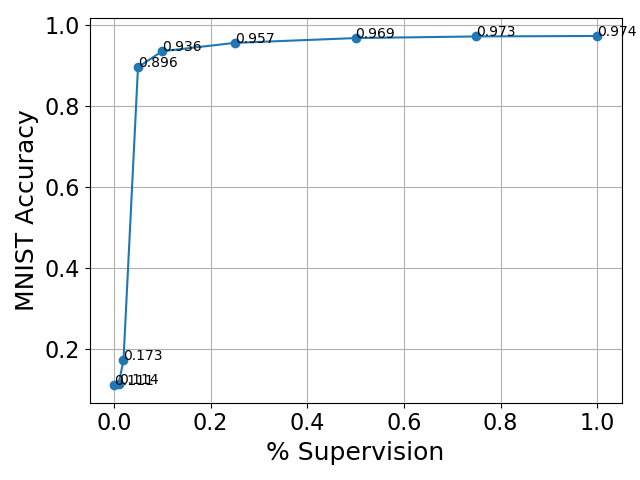
\includegraphics[width=\linewidth]{images/chapter3/mnist.pdf}
    \caption{Dynamic MNIST}
  \end{subfigure}
  \begin{subfigure}[b]{.32\linewidth}
    \centering
    \includegraphics[width=\linewidth]{images/chapter3/fashion.pdf}
    \caption{FashionMNIST}
  \end{subfigure}
  \begin{subfigure}[b]{.32\linewidth}
    \centering
    \includegraphics[width=\linewidth]{images/chapter3/multi.pdf}
    \caption{MultiMNIST}
  \end{subfigure}
  \caption{\textit{Effects of supervision level}. We plot the level of supervision as the log number of paired examples shown to each model. For MNIST and FashionMNIST, we predict the target class. For MultiMNIST, we predict the correct string representing each digit. We compare against a suite of baselines composed of models in relevant literature and commonly used classifiers. MVAE consistently beats all baselines in the \textit{middle region} where there is both enough data to fit a deep model; in the fully-supervised regime, MVAE is competitive with feedforward deep networks. See supplement for accuracies.}
  \label{fig:weaksup_prediction}
\end{figure}

\subsection{Weakly Supervised Learning}
For each dataset, we simulate incomplete supervision by randomly reserving a fraction of the dataset as multi-modal examples. The remaining data is split into two datasets: one with only the first modality, and one with only the second. These are shuffled to destroy any pairing. We examine the effect of supervision on the predictive task $p(x_2|x_1)$, e.g.~predict the correct digit label, $x_2$, from an image $x_1$. For the MVAE, the total number of examples shown to the model is always fixed -- only the proportion of complete bi-modal examples is varied. We compare the performance of the MVAE against a suite of baseline models: (1) supervised neural network using the same architectures (with the stochastic layer removed) as in the MVAE; (2) logistic regression on raw pixels; (3) an autoencoder trained on the full set of images, followed by logistic regression on a subset of paired examples; we do something similar for (4) VAEs and (5) RBMs, where the internal latent state is used as input to the logistic regression; finally (6) we train the JMVAE ($\alpha=0.01$ as suggested in \cite{suzuki2016joint}) on the subset of paired examples. Figure~\ref{fig:weaksup_prediction} shows performance as we vary the level of supervision. For MultiMNIST, $x_2$ is a string (e.g. ``6 8 1 2") representing the numbers in the image. We only include JMVAE as a baseline since it is not straightforward to output raw strings in a supervised manner.

We find that the MVAE surpasses all the baselines on a middle region when there are enough paired examples to sufficiently train the deep networks but not enough paired examples to learn a supervised network. This is especially emphasized in FashionMNIST, where the MVAE equals a fully supervised network even with two orders of magnitude less paired examples (see Figure~\ref{fig:weaksup_prediction}). Intuitively, these results suggest that the MVAE can effectively learn the joint distribution by bootstrapping from a larger set of uni-modal data. A second observation is that the MVAE almost always performs better than the JMVAE. This discrepancy is likely due to directly optimizing the marginal distributions rather than minimizing distance between several variational posteriors. We noticed empirically that in the JMVAE, using the samples from $q(z|x,y)$ did much better (in accuracy) than samples from $q(z|x)$.

\begin{figure}
\centering
    \begin{subfigure}[b]{.49\linewidth}
        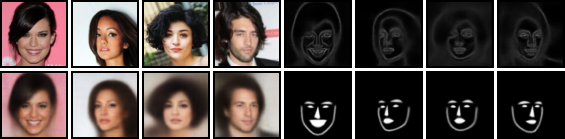
\includegraphics[width=\linewidth]{images/chapter3/vision1_small}
        \caption{Edge Detection and Facial Landscapes}
    \end{subfigure}
    \begin{subfigure}[b]{.49\linewidth}
        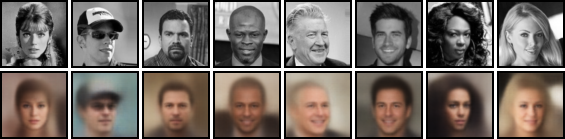
\includegraphics[width=\linewidth]{images/chapter3/colorization}
        \caption{Colorization}
    \end{subfigure}
    \begin{subfigure}[b]{.49\linewidth}
        
\includegraphics[width=\linewidth]{images/chapter3/fill_in_blank}
        \caption{Fill in the Blank}
    \end{subfigure}
    \begin{subfigure}[b]{.49\linewidth}
        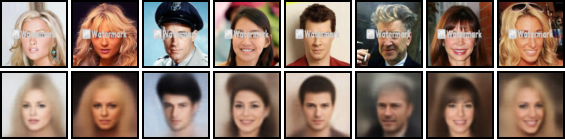
\includegraphics[width=\linewidth]{images/chapter3/watermark}
        \caption{Removing Watermarks}
    \end{subfigure}
    \caption{\textit{Learning Computer Vision Transformations:} (a) 4 ground truth images randomly chosen from CelebA along with reconstructed images, edges, and facial landscape masks; (b) reconstructed color images; (c) image completion via reconstruction; (d) reconstructed images with the watermark removed. }
    \label{fig:vision:images}
\end{figure}

\section{Case study: Computer Vision Applications}
We use the MVAE to learn image transformations (and their inverses) as conditional distributions. In particular, we focus on colorization, edge detection, facial landmark segmentation, image completion, and watermark removal. The original image is itself a modality, for a total of six.

To build the dataset, we apply ground-truth transformations to CelebA. For \textit{colorization}, we transform RGB colors to grayscale. For \textit{image completion}, half of the image is replaced with black pixels. For \textit{watermark removal}, we overlay a generic watermark. To extract edges, we use the Canny detector \cite{canny1987computational} from Scikit-Image \cite{van2014scikit}. To compute facial landscape masks, we use dlib \cite{king2009dlib} and OpenCV \cite{bradski2000opencv}.

We fit a MVAE with 250 latent dimensions and $k {=} 1$. We use Adam with a $10^{-4}$ learning rate, a batch size of 50, $\lambda_{i} = 1$ for $i=1, ..., N$, $\beta$ annealing for 20 out of 100 epochs. Figure~\ref{fig:vision:images} shows samples showcasing different learned transformations. In Figure~\ref{fig:vision:images}a we encode the original image with the learned encoder, then decode the transformed image with the learned generative model. We see reasonable reconstruction, and good facial landscape and edge extraction. In Figs.\ref{fig:vision:images}b, \ref{fig:vision:images}c, \ref{fig:vision:images}d we go in the opposite direction, encoding a transformed image and then sampling from the generative model to reconstruct the original.
The results are again quite good: reconstructed half-images agree on gaze direction and hair color, colorizations are reasonable, and all trace of the watermark is removed.
(Though the reconstructed images still suffer from the same blurriness that VAEs do \cite{zhao2017towards}.)

\section{Case study: Machine Translation}
% \begin{minipage}{\textwidth}
%   \centering
%   \begin{minipage}[h!]{0.49\textwidth}
%     \centering
%       \includegraphics[width=\linewidth]{weaksup/translation.pdf}
%       \label{fig:translation_weaksup}
%   \end{minipage}
%   \hfill
%   \begin{minipage}[b]{0.49\textwidth}
%     \centering
%     \small
%     \begin{tabular}{c|c}
%       \toprule
%       Dataset Size & Test log $p(x)$ \\
%       \hline
%       133 & $-558.88 \pm 3.56$ \\
%       665 & $-494.76 \pm 4.18$\\
%       1330 & $-483.23 \pm 5.81$\\
%       6650 & $-478.75 \pm 3.00$\\
%       13300 & $-478.04 \pm 4.95$\\
%       133000 & $-478.12 \pm 3.02$\\
%       \bottomrule
%     \end{tabular}
%   \end{minipage}
%   \captionof{figure}{\textit{Weakly supervised translation.} We vary the number of paired examples shown to MVAE. With only 1\% of examples being aligned (about 1.3K examples or 7 on the log scale), we see close to equal performance to full supervision. Performance is measured by the log likelihood on a held-out test set, approximated by sampling. Measurements are averaged over 3 runs using 100 samples.}
% \end{minipage}
\begin{table}[h!]
\centering
\begin{tabular}{l|l}
    \toprule
    Num. Aligned Data (\%) & Test log $p(x)$ \\
    \hline
    133 (0.1\%) & $-558.88 \pm 3.56$ \\
    665 (0.5\%) & $-494.76 \pm 4.18$\\
    1330 (1\%) & $-483.23 \pm 5.81$\\
    6650 (5\%) & $-478.75 \pm 3.00$\\
    13300 (10\%) & $-478.04 \pm 4.95$\\
    133000 (100\%) & $-478.12 \pm 3.02$\\
    \bottomrule
\end{tabular}
\caption{\textit{Weakly supervised translation.} Log likelihoods on a test set, averaged over 3 runs. Notably, we find good performance with a small fraction of paired examples.}
\label{table:translation_weaksup}
\end{table}

As a second case study we explore machine translation with weak supervision -- that is, where only a small subset of data consist of translated sentence pairs.
Many of the popular translation models \cite{vaswani2017attention} are fully supervised with millions of parameters and trained on datasets with tens of millions of paired examples.
Yet aligning text across languages is very costly, requiring input from expert human translators.
Even the unsupervised machine translation literature relies on large bilingual dictionaries, strong pre-trained language models, or synthetic datasets \cite{lample2017unsupervised, artetxe2017unsupervised, ravi2011deciphering}. These factors make weak supervision particularly intriguing.

We use the English-Vietnamese dataset (113K sentence pairs) from IWSLT 2015 and treat English (en) and Vietnamese (vi) as two modalities.
We train the MVAE with 100 latent dimensions for 100 epochs ($\lambda_{\textup{en}} = \lambda_{\textup{vi}} = 1$). We use the RNN architectures from \cite{bowman2015generating} with a maximum sequence length of 70 tokens. As in \cite{bowman2015generating}, word dropout and KL annealing are crucial to prevent latent collapse.

\begin{table}[h]
\centering
\scriptsize
\begin{tabular}{ l|l }
  \toprule
  \textbf{Type} & \textbf{Sentence} \\
  % \bottomrule
  % $x_{\textup{en}} \sim p(x_{\textup{en}}|z_0)$ & i'm not kidding . \\
  % $x_{\textup{vi}} \sim p(x_{\textup{vi}}|z_0)$ & \foreignlanguage{vietnamese}{tôi không nói đùa .} \\
  % $\textsc{Google}(x_{\textup{vi}})$ & i am not joking . \\
  % \hline
  % $x_{\textup{en}} \sim p(x_{\textup{en}}|z_0)$ & And as you can see , this is a very powerful effect of word of mouth . \\
  % $x_{\textup{vi}} \sim p(x_{\textup{vi}}|z_0)$ & \foreignlanguage{vietnamese}{và một trong những điều này đã xảy ra với những người khác , và chúng} \\
  % & \foreignlanguage{vietnamese}{tôi đã có một số người trong số các bạn đã từng nghe về những điều này .} \\
  % $\textsc{Google}(x_{\textup{vi}})$ & and one of these has happened to other people, and we've had \\
  % & some of you guys already heard about this . \\
  % $x_{\textup{en}} \sim p(x_{\textup{en}}|z_0)$ & this is a photograph of my life . \\
  % $x_{\textup{vi}} \sim p(x_{\textup{vi}}|z_0)$ & \foreignlanguage{vietnamese}{Đây là một bức ảnh .} \\
  % $\textsc{Google}(x_{\textup{vi}})$ & this is a photo . \\
  % \bottomrule
  $x_{\textup{en}} \sim p_{\textup{data}}$ & this was one of the highest points in my life. \\
  $x_{\textup{vi}} \sim p(x_{\textup{vi}}|z(x_{\textup{en}}))$ & \foreignlanguage{vietnamese}{Đó là một gian tôi vời của cuộc đời tôi.} \\
  $\textsc{Google}(x_{\textup{vi}})$ & It was a great time of my life. \\
  % \hline
  % $x_{\textup{en}} \sim p_{\textup{data}}$ & do you know what love is ? \\
  % $x_{\textup{vi}} \sim p(x_{\textup{vi}}|z(x_{\textup{en}}))$ & \foreignlanguage{vietnamese}{Đó yêu của những ?} \\
  % $\textsc{Google}(x_{\textup{vi}})$ & that's love ?\\
  \hline
  $x_{\textup{en}} \sim p_{\textup{data}}$ & the project's also made a big difference in the lives of the people . \\
  $x_{\textup{vi}} \sim p(x_{\textup{vi}}|z(x_{\textup{en}}))$ & \foreignlanguage{vietnamese}{tôi án này được ra một Điều lớn lao cuộc sống của chúng người sống chữa hưởng .} \\
  % & \foreignlanguage{vietnamese}{sống chữa hưởng .} \\
  $\textsc{Google}(x_{\textup{vi}})$ & this project is a great thing for the lives of people who live and thrive . \\
  \bottomrule
  % $x_{\textup{vi}} \sim p_{\textup{data}}$ & \foreignlanguage{vietnamese}{Đó là thời điểm tuyệt vọng nhất trong cuộc đời tôi .} \\
  % $x_{\textup{en}} \sim p(x_{\textup{en}}|z(x_{\textup{vi}}))$ & this is the most bad of the life . \\
  % $\textsc{Google}(x_{\textup{vi}})$ & it was the most desperate time in my life . \\
  % \hline
  $x_{\textup{vi}} \sim p_{\textup{data}}$ & \foreignlanguage{vietnamese}{trước tiên , tại sao chúng lại có ấn tượng xấu như vậy ?} \\
  $x_{\textup{en}} \sim p(x_{\textup{en}}|z(x_{\textup{vi}}))$ & first of all, you do not a good job ? \\
  $\textsc{Google}(x_{\textup{vi}})$ & First, why are they so bad? \\
  \hline
  $x_{\textup{vi}} \sim p_{\textup{data}}$ & \foreignlanguage{vietnamese}{Ông ngoại của tôi là một người thật đáng <unk> phục vào thời ấy .} \\
  $x_{\textup{en}} \sim p(x_{\textup{en}}|z(x_{\textup{vi}}))$ & grandfather is the best experience of me family . \\
  $\textsc{Google}(x_{\textup{vi}})$ & My grandfather was a worthy person at the time . \\
  \bottomrule
\end{tabular}
% (1) ``paired" reconstructions using $z_0 \sim q(z|x_{\textup{en}}, x_{\textup{vi}})$,
\caption{Examples of (1) translating English to Vietnamese by sampling from $p(x_{\textup{vi}}|z)$ where $z \sim q(z|x_{\textup{en}})$, and (2) the inverse. We use Google Translate (\textsc{Google}) to compute ground-truth translations.}
\label{table:translation_examples}
\end{table}

With only 1\% of aligned examples, the MVAE is able to describe test data almost as well as it could with a fully supervised dataset (Table \ref{table:translation_weaksup}). With 5\% aligned examples, the model reaches maximum performance. Table~\ref{table:translation_examples} shows examples of translation forwards and backwards between English and Vietnamese. See supplement for more examples. We find that many of the translations are not extremely faithful but interestingly capture a close interpretation to the true  meaning. While these results are not competitive to state-of-the-art translation, they are remarkable given the very weak supervision. Future work should investigate combining MVAE with modern translation architectures (e.g.~transformers, attention).

\section{Related Work}
\label{sec:related_work}

Given \textit{two} modalities, $x_{1}$ and $x_{2}$, many variants of VAEs \cite{kingma2013auto, kingma2014semi}  have been used to train generative models of the form $p(x_{2} | x_{1})$, including conditional VAEs (CVAE) \cite{sohn2015learning} and conditional multi-modal autoencoders (CMMA) \cite{pandey2017variational}. Similar work has explored using hidden features from a VAE trained on images to generate captions, even in the weakly supervised setting \cite{pu2016variational}. Critically, these models are not bi-directional. We are more interested in studying models where we can condition interchangeably. For example, the BiVCCA \cite{wang2016deep} trains two VAEs together with interacting inference networks to facilitate two-way reconstruction. However, it does not attempt to directly model the joint distribution, which we find empirically to improve the ability of a model to learn the data distribution.

Several recent models have tried to capture the joint distribution explicitly. \cite{suzuki2016joint} introduced the joint multi-modal VAE (JMVAE), which learns $p(x_{1}, x_{2})$ using a joint inference network, $q(z|x_{1}, x_{2})$. To handle missing data at test time, the JMVAE collectively trains $q(z|x_{1}, x_{2})$ with two other inference networks $q(z|x_{1})$ and $q(z|x_{2})$. The authors use ELBO with two additional divergence terms to minimize the distance between the uni-modal and the multi-modal distributions. Unfortunately, the JMVAE trains a new inference network for each multi-modal subset, which we have previously argue to be intractable in the general setting.

Most recently, \cite{vedantam2017generative} introduce another objective for the bi-modal VAE, which they call the \textit{triplet ELBO}. Like the MVAE, their model's joint inference network $q(z|x_{1}, x_{2})$ combines variational distributions using a product-of-experts rule. Unlike the MVAE, the authors report a two-stage training process: using complete data, fit $q(z|x_{1}, x_{2})$ and the decoders. Then, freezing $p(x_{1}|z)$ and $p(x_{2}|z)$, fit the uni-modal inference networks, $q(z|x_{1})$ and $q(z|x_{2})$ to handle missing data at test time. Crucially, because training is separated, the model has to fit 2 new inference networks to handle all combinations of missing data in stage two. While this paradigm is sufficient for two modalities, it does not generalize to the truly multi-modal case. To the best of our knowledge, the MVAE is the first deep generative model to explore more than two modalities efficiently. Moreover, the single-stage training of the MVAE makes it uniquely applicable to weakly-supervised learning.

Our proposed technique resembles established work in several ways. For example, PoE is reminiscent of a restricted Boltzmann machine (RBM), another latent variable model that has been applied to multi-modal learning \cite{ngiam2011multimodal, srivastava2012multimodal}. Like our inference networks, the RBM decomposes the posterior into a product of independent components. The benefit that a MVAE offers over a RBM is a simpler training algorithm via gradient descent rather than requiring contrastive divergence, yielding faster models that can handle more data. Our sub-sampling technique is somewhat similar to denoising \cite{vincent2008extracting, ngiam2011multimodal} where a subset of inputs are ``partially destructed" to encourage robust representations in autoencoders. In our case, we can think of ``robustness" as capturing the true marginal distributions.

\section{Conclusion}
We introduced a multi-modal variational autoencoder with a new training paradigm that learns a joint distribution and is robust to missing data. By optimizing the ELBO with multi-modal and uni-modal examples, we fully utilize the product-of-experts structure to share inference network parameters in a fashion that scales to an arbitrary number of modalities. We find that the MVAE matches the state-of-the-art on four bi-modal datasets, and shows promise on two real world datasets.

\chapter{Sample Efficiency in Deep Inference}
\label{chapter:antivae}
\section{Introduction}
\label{sec:introduction}
In the last chapter, we investigated the scalability of deep inference with respect to a growing number of data modalities and missing data. Another aspect to the scalability of inference is sample efficiency. Optimizing the ELBO requires computing the gradient of an expectation term, which cannot be evaluated in closed form. Rather, we approximate it with sampling. For instance, in the VAE, we utilize the reparameterization trick \cite{kingma2013auto,rezende2014stochastic} to transform samples from the prior for estimation. For expectations of complex expressions, we may benefit from drawing multiple samples to reduce variance. For instance, the importance weighted autoencoder (IWAE) \cite{burda2015importance} derives a tighter bound on Equation~\ref{eq:marg} using multiple samples. However, additional samples comes at the cost of computation: each additional sample impacts the memory and running time for both the forward and backward pass. For even sophisticated hardware with gigabytes of random-access memory, IWAE is usually limited to fewer than 10 samples. In this chapter, we study a new algorithm for more scalable sampling for use in deep inference.

A wide class of problems in science and engineering can be solved by gradient-based optimization of function expectations.
This is especially prevalent in machine learning \cite{schulman2015gradient},  including variational inference \cite{ranganath2014black, rezende2014stochastic} and reinforcement learning \cite{silver2014deterministic}.
On the face of it, problems of this nature require solving an intractable integral.
Most practical approaches instead use Monte Carlo estimates of expectations and their gradients.
These techniques are unbiased but can suffer from high variance when sample size is small---one unlikely sample in the tail of a distribution can heavily skew the final estimate.
% \rdh{Different estimates from what? I think you can say this more crisply.}
A simple way to reduce variance is to increase the number of samples; however the computational cost grows quickly. We would like to reap the positive benefits of a larger sample size using as few samples as possible. With a fixed computational budget, how do we choose samples?

A large body of work studies reducing variance in sampling, with the most popular in machine learning being  reparameterizations for some continuous distributions \cite{kingma2013auto,jang2016categorical} and control variates to adjust for estimated error \cite{mnih2014neural,weaver2001optimal}.
These techniques sample i.i.d.~but perhaps it is possible to choose correlated samples that are more \textit{representative} of their underlying distribution?
Several such non-independent sampling approaches have been proposed in statistics.
%There are several examples from statistics on the practicality of non-i.i.d sampling; for example, a simple strategy is sampling without replacement, which is forced to be ``representative" by covering the domain more quickly.
% commonly used when drawing from a finite population. \s{$k$ samples without replacement are more representative than with replacement because there can never be duplicates.}
We investigate \textit{antithetics}, where for every sample we draw, we include a negatively correlated sample to minimize the distance between sample and population moments.
% \s{imprecise/incorrect statement i think}. \s{for example, if one sample is much larger than the mean, we will attempt to balance it with one that is much smaller}

The key challenges in applying antithetic sampling to modern machine learning are (1) ensuring that antithetic samples are correctly distributed such that they provide unbiased estimators for Monte Carlo simulation, and (2) ensuring that sampling is differentiable to permit gradient-based optimization.
% \s{key challenge: make sure these samples have the right statistics so that they are still usable in monte carlo schemes and provide unbiased estimators.}
We focus on stochastic variational inference and explore using antithetics for learning the parameters for a deep generative model. %instead of sampling i.i.d.~from the variational posterior, we use an antithetic strategy.
Critically, our method of antithetic sampling is differentiable and can be composed with reparametrizations of the underlying distributions to provide a fully differentiable sampling process. This yields a simple and low variance way to optimize the parameters of the variational posterior.

Concisely, our contributions are as follows: We review a method to to generate Gaussian variates with known sample moments, then apply it to antithetics, and generalize it to other families using deterministic transformations. Seocnd, we show that differentiating through the sampling computation improves variational inference. Finally, we show that training VAEs with antithetic samples improves learning across objectives, posterior families, and datasets.

\section{Preliminaries}
\label{sec:background}

Recall the learning objective for a latent variable model is to maximize the likelihood of the data (the ``evidence"), $\log p_\theta(x)$. This is intractable so we optimize the evidence lower bound (ELBO) instead:
\begin{align}
    \log p_\theta(x) & \geq \mathbf{E}_{q_\phi(z|x)}[\log \frac{p_\theta(x,z)}{q_\phi(z|x)}]\label{eqn:elbo}
    % &= \mathbf{E}_{q_\phi(z|x)}[\log p_\theta(x|z)] - \nonumber \\
    % &\qquad \textup{KL}[\log q_\phi(z|x) || \log p(z)] \label{eqn:elbo-2}
\end{align}
% where KL represents the Kullback-Leibner divergence.
The VAE \cite{kingma2013auto,rezende2014stochastic} is an example of one such generative model where $p_\theta(x|z)$ and $q_\phi(z|x)$ are deep neural networks used to parameterize a simple likelihood.
%As Equation~\ref{eqn:elbo} is a random objective, we can treat it as stochastic optimization.

\begin{comment}
\paragraph{Other Lower Bounds}

\cite{burda2015importance} proposed a popular variant of the ELBO that is a tighter bound on $\log p(x)$, denoted as the IWAE:

\begin{equation}
    \mathbf{E}_{z_1, ..., z_k \sim q_\phi(z|x)}[\log \frac{1}{k} \sum_{i=1}^{k} \frac{p_\theta(x,z_i)}{q_\phi(z_i|x)}]
\label{eqn:iwae}
\end{equation}

Many applications have found the IWAE to give better results than the ELBO.

\paragraph{Flexible Posteriors}

The choice of a Gaussian posterior may not be expressive enough to capture complex distributions (e.g.~multiple modes). \cite{rezende2015variational} improve the flexibility using \textit{normalizing flows} \cite{tabak2010density, tabak2013family}, a technique that applies a series of $T$ invertible transformations $h^{(t)}, t = 1, ..., T$ to samples $z^{(0)}$ from $q_\theta(z|x)$. As a result, the final transformed sample, $z^{(T)}$ comes from a more complex distribution.% To score samples, we choose $h: \mathbf{R}^d \rightarrow \mathbf{R}^d$ carefully such that we can compute the Jacobian-determinant in closed form.
We adjust the objective accordingly:

\begin{align}
    \log p(x) &\geq \mathbf{E}_{z^{(0)} \sim q(z^{(0)}|x)}[\log \frac{p(x,z^{(T)})}{q(z^{(T)}|x)}]
\end{align}

where $q(z^{(T)}|x) = q(z^{(0)}|x) - \log | \det \frac{\partial h^{(t)}}{\partial z^{(t-1)}} |$. \cite{tomczak2016improving} introduces a second family of flows that are \textit{volume preserving}, meaning that the Jacobian-determinant equals 1.

\end{comment}

% Combining flows and smart sampling could lead to better exploration of the new posterior. We will show that matching moments can help learning for a wider family of distributions using flows.

Since $\phi$ can impact the ELBO (though not the true marginal likelihood it lower bounds), we jointly optimize over  $\theta$ and $\phi$.
The gradients of the ELBO objective are:
\begin{align}
    \nabla_\theta \textup{ELBO}(\theta, \phi) &= \mathbf{E}_{z \sim q_\phi(z|x)}[\nabla_\theta \log p_\theta(x,z)] \label{eqn:elbo_gradient_theta} \\
    \nabla_\phi \textup{ELBO}(\theta, \phi) &= \nabla_\phi \mathbf{E}_{z \sim q_\phi(z|x)}[\log \frac{p_\theta(x,z)}{q_\phi(z|x)}]
    \label{eqn:elbo_gradient_phi}
\end{align}
Equation~\ref{eqn:elbo_gradient_theta} can be directly estimated using Monte Carlo. However, as it stands, Equation~\ref{eqn:elbo_gradient_phi} is difficult to approximate as we cannot distribute the gradient inside the expectation. If we constrain $q_\phi(z|x)$ to certain families, we can reparameterize.

% In this section, we present some terminology and summarize the main ideas behind stochastic optimization of functions with respect to \textit{continuous} distributions. Let $x \in \mathbf{R}^{d}$ be a vector of $d$ observable variables and $z \in \mathbf{R}^{l}$ be a vector of $l$ stochastic latent \s{why latent?} variables. We can define an arbitrary function of both variables, $f_{\phi,\theta}(x, z)$, with parameters $\theta$ and $\phi$. Typically, we consider maximizing the following objective:

% \begin{equation}
%     \mathcal{L}(\phi, \theta) = \mathbf{E}_{z \in Q_{\phi}} [f_{\phi,\theta}(x, z)]
% \label{eqn:stochastic_opt}
% \end{equation}
% \s{missing dependence on $x$}

% where $Q$ is a continuous distribution over $z$ parameterized by $\phi$ with a probability density function denoted by $q_\phi(z)$. We assume that $f_{\phi,\theta}(x, z)$ and $q_\phi(z)$ are differentiable with respect to their parameters. To optimize $\mathcal{L}(\phi, \theta)$, we wish to rely on gradient descent, requiring us to efficiently compute the following:

% \begin{equation}
%     \nabla_{\phi, \theta} \mathcal{L}(\phi, \theta) = \mathbf{E}_{z \in Q_\phi}[\nabla_{\phi, \theta} f_{\phi,\theta}(x, z)]
% \label{eqn:gradient_opt}
% \end{equation}

% Given that the domain of $Q_\phi$ can be infinite, $\mathcal{L}(\phi, \theta)$ is intractable to evaluate, and by consequence, to optimize. As a workaround, we settle for approximating the expectation via unbiased Monte Carlo estimates. We now discuss the most popular class of estimators for a subset of continuous distributions.

Reparameterization refers to isolating sampling from the gradient computation graph \cite{kingma2013auto,rezende2014stochastic}. If we can sample $z \sim q_\phi(z|x)$ by applying a deterministic function $z = g_\phi(\epsilon): \mathbf{R}^{d} \rightarrow \mathbf{R}^{d}$ to sampling from an unparametrized distribution, $\epsilon \sim R$, then we can rewrite Equation~\ref{eqn:elbo_gradient_phi} as:
\begin{equation}
    \nabla_\phi \textup{ELBO}(\theta, \phi) = \mathbf{E}_{\epsilon \sim R}[\nabla_z \log\frac{p_\theta(x,z(\epsilon))}{q_\phi(z(\epsilon)|x)} \nabla_\phi g_\phi(\epsilon)]
\label{eqn:gradient_reparam}
\end{equation}

which can now be estimated in the usual manner. As an example, if $q_\phi(z|x)$ is a Gaussian, $N(\mu, \sigma^2)$ and we choose $R$ to be $N(0, 1)$, then $g(\epsilon) = \epsilon * \sigma + \mu$.
% \rdh{confusing because you just said generically $\epsilon \sim R$ -- say here R is a standard normal}
% \ndg{is this notation right?}
% \mwu{made more explicit}
% With reparameterization, maximizing the ELBO is \textit{equivalent} to a stochastic optimization problem (where $Q = q_\phi(z|x)$ and $f(x) = \log p_\theta(x,z) - \log q_\phi(z|x)$). Provided a method of drawing samples from $q$, we can use it to efficiently estimate Equation~\ref{eqn:elbo_gradient_theta} and Equation~\ref{eqn:gradient_reparam}.
% We show below the benefit of doing so using \emph{representative} samples.

% \subsection{Stochastic Optimization}

% Variational inference can be viewed as a specific instance of a broader area of study: stochastic optimization. We can generalize the variational posterior $q_\phi(z|x)$ to a generic distribution $Q$ and the log importance weight as a generic function $f$.

% \ndg{it doesn't make sense to me to formulate it this broadly, because we are only really interested in the case where $Q$ has params that we want gradient wrt....}

% Then generally, the problem of interest is of the form:

% \begin{equation}
%     \min_{\theta} \mathbf{E}_{x\sim Q}[f_{\theta}(x)] = \min_{\theta} \int f_{\theta}(x)dQ(x)
%     \label{eqn:stochastic_opt}
% \end{equation}

% where $f$ is a smooth differentiable function with parameters $\theta$, and $x$ is a function input taken from some distribution $Q$. We are interested in directly minimizing the expectation of $f$. However, because the support of $Q$ can be infinite, evaluation is in general, intractable. Instead, we hope to approximate the expectation by sampling. The gradients with respect to $\theta$ are then given by:

% \begin{equation}
%     \mathbf{E}_{x\sim Q}[\nabla_\theta f_\theta(x)] \approx \frac{1}{k}\sum_{i=1}^{k} Q(x_i)\nabla_\theta f_\theta(x_i)
%     \label{eqn:approx_opt_func}
% \end{equation}
% \ndg{this equation is true, but misleading for the VI case, where we can't move the gradient inside the expectation without re-param...}

% where $x_i \sim Q(x), i=1,...,k$. Notice that Equation~\ref{eqn:approx_opt_func} is exactly the form of Equations~\ref{eqn:elbo_gradient_theta} and \ref{eqn:gradient_reparam}. A sufficiently large variance in Equation~\ref{eqn:approx_opt_func} can lead to ineffective optimization.

\subsection{Antithetic Sampling}
Normally, we sample i.i.d.~from $q_\phi(z|x)$ and $R$ to approximate Equations~\ref{eqn:elbo_gradient_theta} and \ref{eqn:gradient_reparam}, respectively. However, drawing correlated samples could reduce variance in our estimation. Suppose we are given $k$ samples $z_1, z_2, ..., z_{k} \sim q_\phi(z|x)$. We could choose a second set of samples $z_{k+1}, z_{k+2},  ..., z_{2k} \sim q_\phi(z|x, z_1, ..., z_k)$ such that $z_{i+k}$ is somehow the ``opposite" of $z_{i}$. Then, we can write down a new estimator using both sample sets. For example, Equation~\ref{eqn:elbo_gradient_theta} can be approximated by:
% \ndg{doing it as an estimator of expectation objective is ok, but not for the gradient (because of moving the gradient inside)}
\begin{equation}
\frac{1}{2k}\sum_{i=1}^{k} \nabla_\theta \log p_\theta(x, z_i) + \nabla_\theta \log p_\theta(x, z_{i+k})
\label{eqn:opt_antithetic}
\end{equation}
Assuming $z_{k+1}, ..., z_{2k}$ is marginally distributed according to $q_\phi(z|x)$, Equation~\ref{eqn:opt_antithetic} is unbiased. Moreover, if $q_\phi(z|x)$ is near symmetric, the variance of this new estimator will be cut significantly. But what does ``opposite'' mean? One idea is to define ``opposite" as choosing $z_{k+i}$ such that the moments of the combined sample set $z_1, ..., z_{2k}$ match the moments of $q_\phi(z|x)$. Intuitively, if $z_i$ is too large, then choosing $z_{k+i}$ to be too small can help rebalance the sample mean, reducing first order errors. Similarly, if our first set of samples is too condensed at the mode, then choosing antithetic samples with higher spread can stabilize the variance closer to its expectation. However, sampling $z_{k+1}, ..., z_{2k}$ with particular sample statistics in mind is a difficult challenge. To solve this, we first narrow our scope to Gaussian distributions, and later extend to other distribution families.
%We begin by re-introducing a statistical method to draw i.i.d. normal samples with a specified sample mean and variance.

%If $Q$ is close to symmetric, the variance of this new estimator can be cut by a significant fraction while remaining unbiased. Depending on how $x_{k+1}, ..., x_{2k}$ are drawn, the sample moments of the $2k$ samples will approximately match the moments of $Q$.

% \s{i would merge this with VAE section. breaks the flow. you want to transition from stochastic optimization / monte carlo to how to generate these samples.}

% We now briefly discuss two more recent advances with VAEs useful in our own experiments.

% \s{mention somewhere that we start with gaussians, then will extend to other distributions}

\section{Constrained Sampling Problem}
\label{sec:methods}

\begin{figure}
    \centering
    \includegraphics[width=0.35\columnwidth]{images/chapter4/algo_pic.pdf}
    \caption{An illustration of Marsaglia's solution to the constrained sampling problem in two dimensions: build a $(k-1)$-dimensional sphere by intersecting a hyperplane and a $k$-dimensional sphere (each representing a contraint). Generating $k$ samples is equivalent to uniformly sampling from the perimeter of the circle.}
    \label{fig:algo}
\end{figure}

% \s{the idea of matching moments is not necessarily obvious to readers. in fact, not entirely clear that's the best thing to do either. so we need some text justifying this approach} If $Q$ is close to symmetric, . Depending on how $x_{k+1}, ..., x_{2k}$ are drawn, the sample moments of the $2k$ samples will approximately match the moments of $Q$.

% \s{convince readers matching moments is a good idea first}

% \s{as a warmup, might be worth explaining how to match the mean. }
We present a constrained sampling problem: given a Gaussian distribution with population mean $\mu$ and population variance $\sigma^2$, we wish to generate $k$ samples $x_1, ..., x_k \sim N(\mu, \sigma^2)$ subject to the conditions:
%
\begin{align}
    \frac{1}{k}\sum_{i=1}^{k} x_i &= \eta  \label{eqn:constraint1}\\
    \frac{1}{k}\sum_{i=1}^{k} (x_i - \eta)^2 &= \delta^2 \label{eqn:constraint2}
\end{align}
%
where the constants $\eta$ and $\delta^2$ are given and represent the sample mean and sample variance. In other words, how can we draw samples from the correct marginal distribution conditioned on matching desired \emph{sample} moments? For example, we might wish to match sample and population moments: $\eta=\mu$ and $\delta=\sigma$.
% \s{tell people we'll often want $\eta=\mu=$, .., make sure readers realiza there's a difference between sample and population moments.}

Over forty years, there have been a handful of solutions. We review the algorithm introduced by \cite{marsaglia1980c69}. 
% In our experiments, we reference a second algorithm by \cite{pullin1979generation, cheng1984generation}, which is detailed in the supplement. 
We chose \cite{marsaglia1980c69} due its simplicity, low computational overhead, and the fact that it makes the fewest random choices of proposed solutions.

\paragraph{Intuition} Since $x_1, ..., x_k$ are independent, we can write the joint density function:
\begin{equation}
    p(x_1, ..., x_k) = (2\pi \sigma^2)^{-\frac{k}{2}}e^{-\frac{1}{2\sigma^2}\sum_i(x_i - \mu)^2}
\label{eqn:joint_density}
\end{equation}
%Furthermore, we rewrite the constraints as:
%\begin{align}
%    \sum_{i=1}^{k} x_i = k\eta \label{eqn:constraint1}\\
%    \sum_{i=1}^{k} (x_i - \eta)^2 = \gamma^2 \label{eqn:constraint2}
%\end{align}
%where $\gamma = \sqrt{k}\delta$. In this form,
We can interpret Equation~\ref{eqn:constraint1} as a hyperplane and Equation~\ref{eqn:constraint2} as the surface of a sphere in $k$ dimensions. Let $\mathcal{X}$ be the set of all points $(x_1, ..., x_k) \in \mathbf{R}^k$ that satisfy the above constraints. Geometrically, we can view $\mathcal{X}$ as the intersection between the hyperplane and $k$-dimensional sphere, i.e., the surface of a $(k-1)$ dimensional sphere (e.g. a circle if $k=2$).

We make the following important observation: the joint density (Equation~\ref{eqn:joint_density}) is constant for all points in $\mathcal{X}$. To see this, we can write the following:
\begin{equation*}
\begin{split}
    \sum_{i}(x_i - \mu)^2 &= \sum_i(x_i - \eta)^2  + 2(\eta - \mu)\sum_i(x_i - \eta) + k(\eta - \mu)^2 \\
    &= \sum_i(x_i - \eta)^2 + k(\eta - \mu)^2 \\
    &= k \delta^2 + k(\eta - \mu)^2
	%  &= \gamma^2 + k(\eta - \mu)^2
\end{split}
\label{eqn:proof1}
\end{equation*}
where $\sum_i(x_i - \eta) = \sum_i(x_i) - k\eta = 0$ by Equation~\ref{eqn:constraint1}. Plugging this into the density function, rewrite Equation~\ref{eqn:joint_density} as:
\begin{equation}
    p(x_1, ..., x_k) = (2\pi \sigma^2)^{-\frac{k}{2}}e^{-\frac{1}{2\sigma^2}(k \delta^2 + k(\eta - \mu)^2)}
\label{eqn:joint_pdf_2}
\end{equation}
Equation~\ref{eqn:joint_pdf_2} is independent of $x_1, ..., x_k$. For any $(\eta, \delta, \mu, \sigma)$, the density for every $x \in \mathcal{X}$ is constant. In other words, the conditional distribution of $x_1, ..., x_k$ given that $x_1, ..., x_k \in \mathcal{X}$ is the uniform distribution over $\mathcal{X}$. Surprisingly, it does \textit{not} depend on $\mu$ or $\sigma$.
Therefore, to solve the constrained sampling problem, we need only be able to sample uniformly from the surface of a $(k-1)$ dimensional sphere.

\paragraph{Marsaglia's Solution}
More precisely, we can generate the required samples $\textbf{x} = (x_1, ..., x_k)$ from a point $\textbf{z} = (z_1, ..., z_{k-1})$ uniformly distributed on the unit sphere in $\mathbf{R}^{k-1}$ centered at the origin by solving the linear system:
\begin{equation}
    \textbf{x} = k^{\frac{1}{2}}\delta\textbf{z}B + \eta \textbf{v}
\label{eqn:linear_system}
\end{equation}
where $\textbf{v} = (1, 1, ..., 1)$ is a $k$ dimensional vector of ones and $B$ is a $(k-1)$ by $k$ matrix such that the rows of $B$ form an orthonormal basis with the null space of $\textbf{v}$ i.e. we choose $B$ where $BB^{t} = I$ and $B\textbf{v}^{t} = 0$, which happens to satisfy our constraints:
\begin{align}
    \textbf{x}\textbf{v}^t &= k\eta \label{eqn:newc1}\\
    (\textbf{x} - \eta\textbf{v})(\textbf{x} - \eta\textbf{v})^t = k\delta^2\textbf{z}BB^t\textbf{z}^t &= k\delta^2 \label{eqn:newc2}
\end{align}
As $\textbf{z}$ is uniformly distributed over the unit $(k-1)$ sphere, Equation~\ref{eqn:newc1} and \ref{eqn:newc2} guarantee that $\textbf{x}$ is uniformly distributed in $\mathcal{X}$. We can generate $\textbf{z}$ by sampling $(\epsilon_1, ..., \epsilon_{k-1}) \sim N(0, 1)$ and setting $z_i = \epsilon_i / \sum_i \epsilon_i^2$. As in \cite{marsaglia1980c69}, we set $B$ to \textsc{RowNormalize}$(A)$ where $A$ is defined as

\begin{center}
$\begin{bmatrix}
1-k & 1 & 1 & . & . & . & 1 & 1& 1\\
0 & 2-k & 1 & . & . & . & 1 &1 & 1\\
0 &  0 & 3-k & . & . & . & 1 & 1 & 1\\
. &  &  &  &  &  &  & & .\\
 .&  &  &  &  &  &  & & .\\
. &  &  &  &  &  &  & &  .\\
0 & 0 & 0  & . & . & . &-2 & 1 & 1\\
0 & 0  & 0 & . & . &. & 0 &  -1 & 1
\end{bmatrix}$
\end{center}

and \textsc{RowNormalize} is a procedure that divides each row vector in $A$ by the sum of the elements in that row. We summarize Marsaglia's algorithm in Algorithm~\ref{algo:marsaglia} and its properties in Proposition~\ref{prop:marsaglia}.

\begin{figure}
    \centering
    \includegraphics[width=0.5\textwidth]{images/chapter4/algo-marsaglia.png}
    \caption{The \texttt{MarsagliaSample} algorithm.}
    \label{algo:marsaglia}
\end{figure}

\begin{prop}
    For any $k>2$, $\mu \in \mathbf{R}$ and $\sigma^2>0$, if $\eta \sim N(\mu, \frac{\sigma^2}{k})$ and $\frac{(k-1)\delta^2}{\sigma^2} \sim \chi^2_{k-1}$ and $\boldsymbol{\epsilon} = \epsilon_1, ..., \epsilon_{k-1} \sim N(0, 1)$ i.i.d., then the generated samples $x_1, ..., x_k = \textsc{MarsagliaSample}(\boldsymbol{\epsilon}, \eta, \delta^2,k)$ are independent normal variates sampled from $N(\mu, \sigma^2)$ such that $\frac{1}{k}\sum_i x_i = \eta$ and $\frac{1}{k}\sum_i(x_i - \eta)^2 = \delta^2$.
    \label{prop:marsaglia}
\end{prop}
\begin{sketch}We provide a full proof in Section~\ref{sec:proof:anti}. For a sketch, let $\mathbf{x} = (x_1, ..., x_k)$ such that $x_i \sim N(\mu, \sigma^2)$ i.i.d. Compute sample statistics $\eta, \delta^2$ from $\mathbf{x}$ as defined in Equation~\ref{eqn:sample_stats}. Consider the joint distribution over samples and sample moments:
\begin{equation*}
    p(\mathbf{x},\eta,\delta^2) = p(\eta,\delta^2)p(\mathbf{x}|\eta,\delta^2).
\end{equation*}
We make two observations: first, $\eta,\delta^2$, as defined, are drawn from $p(\eta,\delta^2)$. Second, as hinted above, $p(\mathbf{x}|\eta,\delta^2)$ is the uniform distribution over a $(k-1)$-sphere, which Marsaglia shows us how to sample from. Thus, any samples $\mathbf{x'} \sim p(\mathbf{x}|\eta=\eta,\delta^2=\delta^2)$ will be distributed as $\mathbf{x}$ is (marginally), in other words i.i.d. Gaussian.
\end{sketch}

% \s{add some discussion on how to incorporate the population mean and variance. one way to generate $k$ i.i.d. gaussian with specific population mean and variance is to "`randomly pick the constraints"', and then use marsaglia. specifically, sample $\eta$, $\delta^2$ from gaussina, chi-square ...}

As implied in Proposition~\ref{prop:marsaglia}, if we happen to know the population mean $\mu$ and variance $\sigma^2$ (as we do in variational inference given the explicit form of the approximate posterior), we could generate $k$ i.i.d. Gaussian variates by sampling $\eta \sim N(\mu, \frac{\sigma^2}{k})$ and $\frac{(k-1)\delta^2}{\sigma^2} \sim \chi^2_{k-1}$, and passing $\eta$, $\delta^2$ to \textsc{MarsagliaSample}.
% Formally we have the following corollary to Proposition \ref{prop:marsaglia}:
% \s{check $k>2$?}
% \begin{corollary}
%     For any $k>2$, $\mu \in \mathbf{R}$ and $\sigma^2>0$, if $\eta \sim N(\mu, \frac{\sigma^2}{k})$ and $\frac{(k-1)\delta^2}{\sigma^2} \sim \chi^2_{k-1}$ and $\boldsymbol{\epsilon} = \epsilon_1, ..., \epsilon_{k-1} \sim N(0, 1)$, then the generated samples $x_1, ..., x_k = \textsc{MarsagliaSample}(\boldsymbol{\epsilon}, \eta, \delta^2,k)$ are independent normal variates sampled from $N(\mu, \sigma^2)$.
% \label{prop:marsaglia2}
% \end{corollary}

\section{Constrained Antithetic Sampling}

We might be inclined to use \textsc{MarsagliaSample} to directly generate samples with some fixed \emph{deterministic} $\eta=\mu$ and $\delta=\sigma$. However, Proposition~\ref{prop:marsaglia} holds only if the desired sample moments $\eta,\delta$ are \emph{random} variables. If we choose them deterministically, we can no longer guarantee the correct marginal distribution for the samples, thus precluding their use for Monte Carlo estimates. Instead, what we can do is compute $\eta$ and $\delta^2$ from i.i.d. samples from $N(\mu, \sigma^2)$, derive antithetic sample moments, and use \textsc{MarsagliaSample} to generate a second set of samples.

More precisely, given a set of $k$ independent normal variates $(x_1, ..., x_k) \sim N(\mu, \sigma^2)$, we would like to generate a new set of $k$ normal variates $(x_{k+1}, ..., x_{2k})$ such that the combined sample moments match the population moments, $\frac{1}{2k}\sum_{i=1}^{2k} x_i = \mu$ and $\frac{1}{2k}\sum_{i=1}^{2k} (x_i -\mu)^2 = \sigma^2$. We call the second set of samples $(x_{k+1}, ..., x_{2k})$ \textit{antithetic} to the first set. To begin, we compute sample statistics from the first set:
\begin{align}
    \eta &= \frac{1}{k}\sum_{i=1}^{k} x_i & \delta^2 &= \frac{1}{k}\sum_{i=1}^{k} (x_i -\mu)^2
    \label{eqn:sample_stats}
\end{align}
Note that  $\eta,\delta$ are random variables, satisfying $\eta \sim N(\mu, \frac{\sigma^2}{k})$ and $\frac{(k-1)\delta^2}{\sigma^2} \sim \chi^2_{k-1}$. Ideally, we would want the second set to come from an ``opposing" $\eta'$ and $\delta'$. To choose $\eta'$ and $\delta'$, we leverage the \textit{inverse CDF transform}: given the cumulative distribution function (CDF) for a random variable $X$, denoted $F_X$, we can define a uniform variate $Y= F_X(X)$. The \textit{antithetic} uniform variable is then $Y' = 1 - Y$, which upon application of the inverse CDF function, is mapped back to a properly distributed antithetic variate $X' = F^{-1}_X(Y')$. Crucially, $X$ and $X'$ have the same marginal distribution, but are not independent.

Let $F_{\eta}$ represent a Gaussian CDF and $F_{\delta}$ represent a Chi-squared CDF. We can derive $\eta'$ and $\delta'$ as:
\begin{align}
    \eta' &= F^{-1}_\eta(1 - F_\eta(\eta)) \\
    \frac{(k-1)(\delta')^2}{\sigma^2} &= F^{-1}_\delta\left(1 - F_\delta \left(\frac{(k-1)\delta^2}{\sigma^2}\right)\right) \label{eq:inversechi}
\end{align}
Crucially, $\eta', \delta'$ chosen this way are random variables with the correct marginal distributions, i.e., $\eta' \sim N(\mu, \frac{\sigma^2}{k})$ and $\frac{(k-1)(\delta')^2}{\sigma^2} \sim \chi^2_{k-1}$. knowing $\eta', \delta'$, it is straightforward to generate antithetic samples with \textsc{MarsagliaSample}. We summarize the algorithm in Algorithm~\ref{alg:antithetic} and its properties in Proposition~\ref{prop:antithetic}.

\begin{figure}
    \centering
    \includegraphics[width=0.5\textwidth]{images/chapter4/algo-antithetic.png}
    \caption{The \texttt{AntitheticSample} algorithm.}
    \label{alg:antithetic}
\end{figure}
% \begin{algorithm}[h!]
% \SetAlgoLined
% \caption{\textsc{AntitheticSample}}
% \KwData{i.i.d. samples $(x_1, ..., x_k) \sim N(\mu, \sigma^2)$; i.i.d. samples $\boldsymbol{\epsilon} = (\epsilon_1, ..., \epsilon_{k-1}) \sim N(0, 1)$; Population mean $\mu$ and variance $\sigma^2$; Number of samples $k \in \mathbf{N}$.} % \s{k}
% \KwResult{A set of $k$ samples $(x_{k+1}, x_{k+2}, ..., x_{2k})$ marginally distributed as $N(\mu, \sigma^2)$ with sample mean $\eta'$ and sample standard deviation $\delta'$.}

% $v = k -1$\;
% $\eta = \frac{1}{k}\sum_{i=1}^k x_i$\;
% $\delta^2 = \frac{1}{k}\sum_{i=1}^k (x_i - \eta)^2$\;
% % $\eta' = 2\mu - \eta$\;
% $\eta' = F^{-1}_\eta(1 - F_\eta(\eta))$\;
% $\lambda = v\delta^2/\sigma^2$\;
% $\lambda' = F^{-1}_\delta(1 - F_\delta(\lambda))$\;
% % $\lambda' = v(2(1 - \frac{3}{16v} - \frac{7}{512v^2} + \frac{231}{8192v^3}) - (\frac{\lambda}{v})^{1/4})^4$\;
% $(\delta')^2 = \lambda'\sigma^2/v$\;
% $(x_{k+1}, ..., x_{2k}) = \textsc{MarsagliaSample}(\boldsymbol{\epsilon}, \eta', (\delta')^2, k)$\;
% Return $(x_{k+1}, ..., x_{2k})$\;
% \label{alg:antithetic}
% \end{algorithm}

% \s{not sure we can make any claim on the sample variance. even if the chi-square thing was exact, not clear to me the variance would match exactly}
\begin{prop}
Given $k - 1$ i.i.d samples $\boldsymbol{\epsilon} = (\epsilon_1, ..., \epsilon_{k-1}) \sim N(0, 1)$, $k$ i.i.d. samples $\boldsymbol{x} = (x_1, ..., x_k) \sim N(\mu, \sigma^2)$, let $(x_{k+1}, ..., x_{2k}) = \textsc{AntitheticSample}(\boldsymbol{x}, \boldsymbol{\epsilon}, \mu, \sigma^2, k)$ be the generated antithetic samples. Then:
\begin{enumerate}
\item $x_{k+1}, ..., x_{2k}$ are independent normal variates sampled from $N(\mu, \sigma^2)$.
\item The combined sample mean $\frac{1}{2k}\sum_{i=1}^{2k}x_i$ is equal to the population mean $\mu$.
\item The sample variance of $x_{k+1}, ..., x_{2k}$ is anticorrelated with the sample variance of $x_1, ..., x_k$.
\end{enumerate}
%i.i.d. but each $x_{k+i}$ is negatively correlated with $x_{i}$. The combined sample mean $\frac{1}{2k}\sum_{i=1}^{2k}x_i = \mu$ will match the population mean. The combined sample variance $\frac{1}{2k}\sum_{i=1}^{2k}(x_i-\mu)^2 = \sigma^2$ will match population variance.
% The total sample variance $\frac{1}{2k}\sum_{i=1}^{2k}(x_i - \mu)^2 \approx \sigma^2$ will be close to the population variance (depending on the normal approximation error).
\label{prop:antithetic}
\end{prop}
\begin{proof}
The first property follows immediately from Proposition~\ref{prop:marsaglia}, as by construction $\eta', \delta'$ have the correct marginal distribution. Simple algebra shows that the inverse Gaussian CDF transform simplifies to $\eta' = 2 * \mu - \eta$, giving the desired relationship $\eta/2 + \eta'/2 = \mu $. The third property follows from Equation \ref{eq:inversechi}.
\end{proof}

Since both sets of samples share the same (correct) marginal distribution, $x_1, ..., x_{2k}$ can be used to obtain unbiased Monte Carlo estimates.
% \s{try to make the proof more precise, actually write down the expectation with respect to the joint. in the proof, use previous result that the samples have the right marginal distribution. that is the key step..}
\begin{prop}
    %For a normal distribution $Q$, given $x_1, ..., x_k \sim Q$ i.i.d. samples and $x_{k+1}, ..., x_{2k}$ i.i.d. antithetic samples drawn using $\textsc{AntitheticSample}$, the combined set $(x_1, ..., x_{2k})$ forms an unbiased estimator, $\frac{1}{2k}\sum_{i=1}^{2k} f_\theta(x_i)Q(x_i)$ for a generic expectation, $\mathbf{E}_{x \sim Q}[f_\theta(x)]$ of a function $f$.
		Given $k - 1$ i.i.d samples $\boldsymbol{\epsilon} = (\epsilon_1, ..., \epsilon_{k-1}) \sim N(0, 1)$, $k$ i.i.d. samples $\boldsymbol{x} = (x_1, ..., x_k) \sim N(\mu, \sigma^2)$, let $(x_{k+1}, ..., x_{2k}) = \textsc{AntitheticSample}(\boldsymbol{x}, \boldsymbol{\epsilon}, \mu, \sigma^2, k)$ be the generated antithetic samples. Then $\frac{1}{2k} \sum_{i=1}^{2k} f(x_i)$ is an unbiased estimator of $\mathbf{E}_{x \sim N(\mu, \sigma^2)}[f(x)]$.
 \label{unbiased}
\end{prop}

\begin{proof}
Let $q(x_1, \cdots, x_k, x_{k+1}, \cdots, x_{2k})$ denote the joint distribution of the $2k$ samples. Note the two groups of samples $(x_1, ..., x_k)$ and $(x_{k+1}, ..., x_{2k})$ are not independent. However,
\begin{align*}
\mathbf{E}_{(x_1, \cdots, x_k, x_{k+1}, \cdots, x_{2k}) \sim q} \left[ \frac{1}{2k} \sum_{i=1}^{2k} f(x_i) \right] = \\
\frac{1}{2k} \sum_{i=1}^{2k} \mathbf{E}_{x_i \sim q_i(x_i)} \left[f(x_i) \right] = \mathbf{E}_{x \sim N(\mu, \sigma^2)}[f(x)]
\end{align*}
because by assumption and Proposition~\ref{prop:antithetic}, each $x_i$ is marginally distributed as $N(\mu, \sigma^2)$.
%We can define an estimator using only the first $k$ samples, $e_1 = \frac{1}{k}\sum_{i=1}^{k} f_\theta(x_i)Q(x_i)$. By definition, $e_1$ is unbiased. Similarly, we define a second estimator using the next $k$ samples, $e_2 = \frac{1}{k}\sum_{i=k+1}^{2k} f_\theta(x_i)Q(x_i)$. By Proposition~\ref{prop:antithetic}, $x_{k+1}, ..., x_{2k} \sim Q$ are marginally distributed according to $Q$. Therefore, $e_2$ is also unbiased. We write the combined estimator as $\frac{1}{2k}\sum_{i=1}^{2k} f_\theta(x_i)Q(x_i) = \frac{e_1}{2} + \frac{e_2}{2}$. A linear combination of two unbiased estimators is unbiased.
\label{prop:test}
\end{proof}

\subsection{Approximate Antithetic Sampling}

If $F_\eta$ and $F_\delta$ were well-defined and invertible, we could use Algorithm~\ref{alg:antithetic} as is, with its good guarantees. On one hand, since $\eta$ is normally distributed, the inverse CDF transform simplifies to:
\begin{equation}
    \eta' = 2 * \mu - \eta
\label{eqn:inversecdf_mean}
\end{equation}
However, there is no general closed form expression for $F^{-1}_\delta$. Our options are then to either use a discretized table of probabilities or approximate the inverse CDF. Because we desire differentiability, we choose to use a normal approximation to $F_{\delta}$.

\paragraph{Antithetic Hawkins-Wixley}

\cite{canal2005normal} surveys a variety of normal approximations, all of which are a linear combination of $\chi^2$ variates to a power root. We choose to use \cite{hawkins1986note} as (P1) it is an even power, (P2) it contains only 1 term involving a random variate, and (P3) is shown to work better for smaller degrees of freedom (smaller sample sizes). We derive a closed form for computing $\delta'$ from $\delta$ by combining the normal approximation with Equation~\ref{eqn:inversecdf_mean}. We denote this final transform as the \textit{antithetic Hawkins-Wixley transform}:
\begin{equation}
    \lambda' = v(2(1 - \frac{3}{16v} - \frac{7}{512v^2} + \frac{231}{8192v^3}) - (\frac{\lambda}{v})^{1/4})^4
    \label{eqn:anti_approx}
\end{equation}
where $\lambda \sim \chi^2_{v}$ with $v$ being the degree of freedom. Therefore, if we set $\lambda = (k-1)\delta^2/\sigma^2 \sim \chi^2_{k-1}$ and $v = k - 1$, then we can derive $(\delta')^2 = \lambda'\sigma^2/(k-1)$ where $\lambda'$ is computed as in Equation~\ref{eqn:anti_approx}, whose derivation can be found in Section~\ref{sec:proof:anti}.

P1 is important as odd degree approximations e.g. \cite{wilson1931distribution} can result in a negative value for $\lambda'$ under small $k$. P2 is required to derive a closed form as most linear combinations do not factor. P3 is desirable for variational inference.

To update Algorithm~\ref{alg:antithetic}, we swap the fourth line with Equation~\ref{eqn:inversecdf_mean} and the sixth line with Equation~\ref{eqn:anti_approx}.
The first property in Proposition \ref{prop:antithetic} and therefore also Proposition \ref{unbiased} do not hold anymore: the approximate \textsc{AntitheticSample} has bias that depends on the approximation error in Equation~\ref{eqn:anti_approx}.
%
%We summarize the properties of the approximate antithetic sampler below:
%\begin{prop}
%Given $k - 1$ i.i.d samples $\boldsymbol{\epsilon} = (\epsilon_1, ..., \epsilon_{k-1}) \sim N(0, 1)$, $k$ i.i.d. samples $\boldsymbol{x} = (x_1, ..., x_k) \sim N(\mu, \sigma^2)$, the generated samples $(x_{k+1}, ..., x_{2k}) = \textsc{AntitheticSample}(\boldsymbol{x}, \boldsymbol{\epsilon}, \mu, \sigma^2, k)$ are i.i.d. but each $x_{k+i}$ is negatively correlated with $x_{i}$. The combined sample mean $\frac{1}{2k}\sum_{i=1}^{2k}x_i = \mu$ will match the population mean. The samples $x_1, ..., x_{2k}$ no longer form an unbiased estimator with error dependent on the approximation error in Equation~\ref{eqn:anti_approx}.
%\label{prop:antithetic2}
%\end{prop}
In practice, we find the approximate \textsc{AntitheticSample} to be effective.
From now on, when we refer to \textsc{AntitheticSample}, we refer to the approximate version. We refer to Figure~\ref{fig:demo} for an illustration of the impact of antithetics: sampling i.i.d. could result in skewed sample distributions that over-emphasize the mode or tails, especially when drawing very few samples. Including antithetic samples helps to ``stabilize" the sample distribution to be closer to the true distribution.


\begin{figure}[h!]
    \centering
    \begin{subfigure}[b]{\columnwidth}
        \includegraphics[width=\columnwidth]{images/chapter4/demo_legend.pdf}
    \end{subfigure}
    \begin{subfigure}[b]{.24\columnwidth}
        \includegraphics[width=\columnwidth]{images/chapter4/demo8sample.pdf}
        \caption{$k=8$}
        \label{fig:demo8}
    \end{subfigure}
    \begin{subfigure}[b]{.24\columnwidth}
        \includegraphics[width=\columnwidth]{images/chapter4/demo10sample.pdf}
        \caption{$k=10$}
        \label{fig:demo10}
    \end{subfigure}
    \begin{subfigure}[b]{.24\columnwidth}
        \includegraphics[width=\columnwidth]{images/chapter4/demo20sample.pdf}
        \caption{$k=20$}
        \label{fig:demo20}
    \end{subfigure}
    \begin{subfigure}[b]{.24\columnwidth}
        \includegraphics[width=\columnwidth]{images/chapter4/demo50sample.pdf}
        \caption{$k=50$}
        \label{fig:demo50}
    \end{subfigure}
    \caption{The effect of \textsc{AntitheticSample} in 1 dimension. We vary the number of samples $k$, and plot the true distribution (solid black line), a kernel density estimate (KDE) of the empirical distribution (dotted blue line) of $2k$ i.i.d. samples (blue), and a KDE of the empirical distribution (dashed red line) of $k$ i.i.d. samples (red) pooled with $k$ antithetic samples (orange).
%    The ``+" and ``x" symbols in each figure represent the raw samples. With smaller $k$, the red curve is a much closer approximation of the black curve than its blue counterpart. As $k$ increases, both sampling techniques converge on the true distribution.
    This snapshot was taken from the first epoch of training an AntiVAE on dynamic MNIST.}

    % \rdh{I wonder whether a more schematic version of this can go earlier in the intro to motivate the intuition? also, make the lines thinker and the sample markers on the x axis a lot bigger so you can see them. also, it looks like the true distribution is different across the columns? (it's taller)}}
        % \s{needs better captioning and legend. unclear what is shown. also not readable in black and white}
    \label{fig:demo}
\end{figure}

% Alternatively, \cite{cheng1982use, cheng1984generation} proposes an antithetic sampling technique using \textsc{MatchMoments}. Given $X \sim N(\mu, \sigma^2)$, derive \textit{antithetic} moments from the moments of $X$. Largely, this involves applications of the inverse-CDF trick and normal approximations for non-normal variates, resulting in a second set of antithetic samples $X'$ such that when used in combination with $X$, should help reduce first order errors. In practice, we find the normal approximations to be poor, resulting in little difference in estimator quality. We find directly matching moments to be much simpler and more effective. \s{i don't understand this paragraph}

% \ndg{is it at all feasible to have a theorem showing that variance of an expectation estimate will be strictly lower after matching moments (under some appropriately draconian assumptions)?}

% \mwu{my gut instinct is that this depends a lot on the function in the expectation.}

\section{Generalization to Other Families}
\label{sec:generalization}

% \s{be explicit about what you get here. you are not matching the moments of the resulting distribution. it's a bit of a weird thing..}

Marsaglia's algorithm is restricted to distribution families that can be transformed to a unit sphere (primarily Gaussians), as are many similar algorithms \cite{cheng1984generation, pullin1979generation}. However, we can explore ``generalizing" \textsc{AntitheticSample} to a wider class of families by first antithetically sampling in a Gaussian distribution, then transforming its samples to samples from another family using a deterministic function, $g: \mathbf{R}^d \rightarrow \mathbf{R}^d$. Although we are not explicitly matching the moments of the derived distributions, we expect that transformations of more representative samples in an initial distribution may be more representative in the  transformed distribution. We now discuss a few candidates for $g(\cdot)$.

\subsection{One-Liners}
\cite{devroye1996random} presents a large suite of ``one line" transformations between distributions. We focus on three examples starting from a Gaussian to (1) Log Normal, (2) Exponential, and (3) Cauchy. Many additional transformations (e.g.~to Pareto, Gumbel, Weibull, etc.) can be used in a similar fashion. Let $F_x$ refer to the CDF of a random variable $x$. See Section~\ref{sec:proof:anti} for derivations.

% \begin{figure}[h!]
%     \centering
%     \begin{subfigure}[b]{\columnwidth}
%         \includegraphics[width=\columnwidth]{skematic2.pdf}
%         \caption{}
%         \label{fig:skematic2}
%     \end{subfigure}
%     \begin{subfigure}[b]{\columnwidth}
%         \includegraphics[width=\columnwidth]{skematic3.pdf}
%         \caption{}
%         \label{fig:skematic3}
%     \end{subfigure}
%     \caption{Composition of a series of transformations on samples from $q(z|x)$. In (a), \textsc{MatchMoments} is applied prior to reparameterization so it escapes the backwards pass. In (b) \textsc{MatchMoments} is included in backpropagation. $g(z)$ represents a series of transformations e.g. one liners, flows, etc.}
% \end{figure}


\paragraph{Log Normal}$g(z) = e^z$ where $z \sim N(\mu, \sigma^2)$.
% For this example, we can apply $g$ after \textsc{MatchMoments} and backpropagate.

% \paragraph{Inverse CDF transform} More complex one liners (again) operate via the inverse CDF transform.  Let $F_x$ denote the CDF for a variable $x$, then $y = F_x(x)$ where $y \in U(0, 1)$. We can derive the inverse transformation $F_x^{-1}(y)$ by solving the system: $F_x(F_x^{-1}(y)) = y$. This allows us to map a Gaussian variate to a Uniform, which can then be mapped to many families.

% With this, the variational posterior is no longer Gaussian: the computational flow becomes 1) sample from a unit Gaussian, 2) apply \textsc{MatchMoments}, 3) map to Uniform, 4) apply some $g$ to map to a final distribution. Thus, we no longer backpropagate through \textsc{MatchMoments}. \s{is there a way to do it with adjoints?}

\paragraph{Exponential} Let $F_x(x) = 1 - \exp^{\lambda x}$ where $\lambda\in \mathbf{R}^d$ is a learnable parameter. Then $F_x^{-1}(y) = -\frac{1}{\lambda} \log y$. Thus, $g(u, \lambda) = -\frac{1}{\lambda} \log u$ where $u \in U(0, 1)$.

\paragraph{Cauchy} Let $F_x(x) = \frac{1}{2} + \frac{1}{\pi}\arctan(\frac{x - x_0}{\gamma})$ where $x_0\in \mathbf{R}^d, \gamma\in \mathbf{R}^d$ are learnable parameters. Then $F_x^{-1}(y) = \gamma(\tan(\pi y) + x_0)$. Given $u \in U(0, 1)$, we define $g(u, x_0, \gamma) = \gamma(\tan(\pi u) + x_0)$.


\subsection{Deeper Flows}
One liners are an example of a simple flow where we know how to score the transformed sample. If we want more flexible distributions, we can apply normalizing flows (NF). A \textit{normalizing flow} \cite{rezende2015variational} applies $T$ invertible transformations $h^{(t)}, t = 1, ..., T$ to samples $z^{(0)}$ from a simple distribution, leaving $z^{(T)}$ as a sample from a complex distribution. A common normalizing flow is a linear-time transformation: $g(z) = z + u(h(w^{T}z + b))$ where $w\in \mathbf{R}^d, u\in \mathbf{R}^d, b\in \mathbf{R}$ are learnable parameters, and $h$ is a non-linearity. In variational inference, flows enable us to parameterize a wider set of posterior families.
% This particular $g(\cdot)$ is easy to use as its Jacobian-determinant can be computed in closed form: $|\det \frac{\partial g}{\partial z}| = |1 + u^{T}h'(w^{T}z + b)w|$.

We can also achieve flexible posteriors using volume-preserving flows (VPF), of which \cite{tomczak2016improving} introduced the Householder transformation: $g(z) = (I - 2\frac{v \cdot v^T}{\|v\|^2})z$ where $v \in \mathbf{R}^d$ is a trainable parameter. Critically, the Jacobian-determinant is 1.

\begin{figure}
    \centering
    \includegraphics[width=0.5\textwidth]{images/chapter4/algo-antivae.png}
    \caption{The AntiVAE inference algorithm.}
    \label{algo:vae_forward}
\end{figure}
% often set to the output of a hidden layer in the inference network
% \begin{algorithm}[h]
% \SetAlgoLined
% \caption{AntiVAE Inference}
% \KwData{A observation $x$; number of samples $k \geq 6$; a variational posterior $q(z|x)$ e.g. a $d$-dimensional Gaussian, $N^d(\mu, \sigma^2)$.}
% \KwResult{Samples $z^d_1,...,z^d_k\sim q_{\mu, \sigma}(z|x)$ that match moments.}
% $\mu^d$, $\sigma^d =$\textsc{InferenceNetwork}$(x)$\;
% $\mu = \normalfont\textsc{Flatten}(\mu^d)$\;
% $\sigma = \normalfont\textsc{Flatten}(\sigma^d)$\;
% $\epsilon_1, ..., \epsilon_{kd/2} \sim N(0, 1)$\;
% $\boldsymbol{\xi} = \xi_1, ..., \xi_{\frac{kd}{2} - 1} \sim N(0, 1)$\;
% \For{$i\gets 1$ \KwTo $kd/2$}{
%     $y_i = \epsilon_i * \sigma + \mu$\;
% }
% $\boldsymbol{y} = (y_1, ..., y_{kd/2})$\;
% $y_{\frac{kd}{2} + 1}, ..., y_{kd} = $\textsc{AntitheticSample}$(\boldsymbol{y}, \boldsymbol{\xi}, \mu, \sigma)$\;
% $\boldsymbol{z} = (y_1, ..., y_{kd})$\;
% $z^d_1, ..., z^d_k = \normalfont\textsc{UnFlatten}(\boldsymbol{z})$\;
% Return $z^d_1, ..., z^d_k$\;
% \label{algo:vae_forward}
% \end{algorithm}

\section{Differentiable Antithetic Sampling}

% \s{now the issue is that reviewers will (correctly) say this is not new because it's in cheng's papers. i think we want to be explicit about what's new. we can probably claim we are the first to backprop through. we can claim we are the first to apply to variational inference. maybe the one-liners? anything else? anyways, i think some separate section with the new stsuff would be helpful. and if possible, i wouldn't tie it to the VAE case. explain the new stuff in the context of general stochastic optimization and variational inference. that will make it cleaner and more general. basically, try to distill what's new, and make a bigger deal out of it..}

% \s{for example, explain how you would backprop through matchmoments, and with respect to what, and is it even differentiable (doesn't look differentiable to me..), etc.}

% \ndg{i don't love starting at stochastic optimization in general, because what is cool here is that using matchmoments in elbo allows the gradient to be passed through (its a reparam). what do you think about focussing this section on VI? the flow is then: elbo estimated with samples from matchmoments+transform is still an unbiased lower bound estimate, because matchmoments is differentiable the elbo gradients can be simply derived (ala reparam), the computation can be done by AD.}
Finally, we can use \textsc{AntitheticSample} to approximate the ELBO for variational inference.
For a given observation $x \in p_\textup{data}$ from an empirical dataset, we write the antithetic gradient estimators as:
\begin{equation}
    \begin{split}
        \nabla_\theta \textup{ELBO}(\theta, \phi) &\approx \frac{1}{2k}\sum_{i=1}^{k}[\nabla_\theta \log p_\theta(x, z_i) \\
        & + \nabla_\theta \log p_\theta(x, z_{i+k}) ]\label{eqn:grad_anti1}
    \end{split}
\end{equation}
\begin{equation}
    \begin{split}
        \nabla_\phi \textup{ELBO}(\theta, \phi) &\approx \frac{1}{2k}\sum_{i=1}^{k}[\nabla_{z} \log \frac{p_\theta(x, z_i(\epsilon))}{q_\phi(z_i(\epsilon)|x)}\nabla_\phi g_\phi(\epsilon_i) \\
        & + \nabla_{z} \log \frac{p_\theta(x, z_{i+k}(\epsilon))}{q_\phi(z_{i+k}(\epsilon)|x)}\nabla_\phi g_\phi(\epsilon_{i+k})]\label{eqn:grad_anti2}
    \end{split}
\end{equation}
where $(\epsilon_1, ..., \epsilon_k) \sim N(0, 1)$, $\boldsymbol{\xi} = (\xi_1, ..., \xi_{k-1})$, $\boldsymbol{z} = (z_1, ..., z_k) \sim q_\phi(z|x)$, and $(z_{k+1}, ..., z_{2k}) = \textsc{AntitheticSample}(\boldsymbol{z}, \boldsymbol{\xi}, \mu, \sigma^2, k)$. Optionally, $\boldsymbol{z} = \textsc{Transform}(\boldsymbol{z}, \alpha)$ where $\textsc{Transform}$ denotes any sample transformation(s) with parameters $\alpha$.

Alternative variational bounds have been considered recently, including an importance-weighted estimator of the ELBO, or IWAE \cite{burda2015importance}. Antithetic sampling can be applied in a similar fashion, as also shown in~\cite{shu2019buffered}.

Importantly, \textsc{AntitheticSample} is a special instance of a reparameterization estimator. Aside from samples from a parameter-less distribution (unit Gaussian), \textsc{AntitheticSample} is completely deterministic, meaning that it is differentiable with respect to the population moments $\mu$ and $\sigma^2$ by any modern auto-differentiation library.
% \begin{figure}[h!]
%     \begin{subfigure}[b]{0.49\columnwidth}
%         \includegraphics[width=\columnwidth]{vae_trajectory.pdf}
%         \caption{VAE}
%         \label{fig:vae_traj}
%     \end{subfigure}
%     \begin{subfigure}[b]{0.49\columnwidth}
%         \includegraphics[width=\columnwidth]{matchae_trajectory.pdf}
%         \caption{AntiVAE}
%         \label{fig:antivae_traj}
%     \end{subfigure}
% \caption{Trajectory of first 100 epochs for variational posteriors $q(z|x)$ for a fixed observation $x$ from dynamic MNIST with $|z| = 2$. With a fixed random seed, same weight initialization, and same number of random choices, we find that adding antithetic sampling finds a different local maxima.}
% \rdh{hmm, i'm not sure what this is showing. first, are these exactly the same latent dimensions? why does the red mean? why is it significant that it finds a different local maxima (i.e. without characterizing what is special about these two maxima?}}
% \label{fig:q_trajectory}
% \end{figure}
%This is special as usually, in variational inference, learning $\phi,\theta$ is isolated from the sample generation.
Allowing backpropagation through \textsc{AntitheticSample} means that any free parameters are aware of the sampling strategy. Thus, including antithetics will change the optimization trajectory, resulting in a different variational posterior than if we had used i.i.d  samples alone. In Sec.~\ref{sec:results}, we show experimentally that \textit{most of the benefit} of differentiable antithetic sampling comes from being differentiable.

% \mwu{its probably unbiased. need to add proof.}
Algorithm~\ref{algo:vae_forward} summarizes inference in a VAE using differentiable antithetic sampling (denoted by AntiVAE). In our experiments, we compare Marsaglia's to a competing algorithm by Cheng \cite{cheng1982use}. We refer to this as AntiVAE (Cheng).
To the best of our knowledge, the application of antithetic sampling to stochastic optimization, especially variational inference is novel. Both the application of \cite{marsaglia1980c69} to drawing antithetics and the extension of \textsc{AntitheticSample} to other distribution families by transformation is novel. This is also the first instance of differentiating through an antithetic sample generator.
% \ndg{This stuff is hanging out of place...: \textsc{Flatten} reshapes a matrix of size $k$ by $d$ to a vector of $k * d$. \textsc{UnFlatten} is the inverse. With diagonal covariance, 1 sample from a $d$ dimensional Gaussian is equivalent to $d$ samples from a 1 dimensional Gaussian.}
\begin{figure*}[t!]
    \centering
    \begin{subfigure}[b]{\textwidth}
        \includegraphics[width=\textwidth]{images/chapter4/elbo_legend.pdf}
    \end{subfigure}
    \begin{subfigure}[b]{0.135\textwidth}
        \includegraphics[width=\textwidth]{images/chapter4/static_mnist_main_result.pdf}
        \caption{static}
        \label{fig:elbo_static_mnist}
    \end{subfigure}
    \begin{subfigure}[b]{0.135\textwidth}
        \includegraphics[width=\textwidth]{images/chapter4/dynamic_mnist_main_result.pdf}
        \caption{dynamic}
        \label{fig:elbo_dynamic_mnist}
    \end{subfigure}
    \begin{subfigure}[b]{0.135\textwidth}
        \includegraphics[width=\textwidth]{images/chapter4/fashion_mnist_main_result.pdf}
        \caption{Fashion}
        \label{fig:elbo_fashion_mnist}
    \end{subfigure}
    \begin{subfigure}[b]{0.135\textwidth}
        \includegraphics[width=\textwidth]{images/chapter4/omniglot_main_result.pdf}
        \caption{Omniglot}
        \label{fig:elbo_omniglot}
    \end{subfigure}
    \begin{subfigure}[b]{0.135\textwidth}
        \includegraphics[width=\textwidth]{images/chapter4/caltech_main_result.pdf}
        \caption{Caltech}
        \label{fig:elbo_caltech}
    \end{subfigure}
    \begin{subfigure}[b]{0.135\textwidth}
        \includegraphics[width=\textwidth]{images/chapter4/freyfaces_main_result.pdf}
        \caption{Frey}
        \label{fig:elbo_freyfaces}
    \end{subfigure}
    \begin{subfigure}[b]{0.135\textwidth}
        \includegraphics[width=\textwidth]{images/chapter4/histopathology_main_result.pdf}
        \caption{Hist.}
        \label{fig:elbo_histopathology}
    \end{subfigure}
\caption{A comparison of test log likelihoods over 500 epochs between VAE and AntiVAE. Transforming samples to match moments seems to have different degrees of effectiveness depending on the data domain. However, we find that the test ELBO with AntiVAE is almost always greater or equal to that of the VAE. This behavior is not sensitive to hyperparameters e.g. learning rate or MLP hidden dimension. For each subplot, we start plotting from epoch 20 to 500. We cannot resample observations in Caltech101, leading to overfitting.}
\label{fig:learning_trajectory}
\end{figure*}

\begin{table*}[t!]
\scriptsize
\begin{tabular}{r|ccccccc}
    Model & stat. MNIST & dyn. MNIST & FashionMNIST & Omniglot & Caltech  & Frey & Hist. \\
    \toprule
    VAE & -90.44 & -86.96 & -2819.13 & -110.65 & -127.26 & -1778.78 & -3320.37\\
    AntiVAE & -89.74 & -86.94 & -2807.06 & \textbf{-110.13} & \textbf{-124.87} & -1758.66 & -3293.01 \\
    AntiVAE (Cheng) & \textbf{-89.70} & \textbf{-86.93} & \textbf{-2806.71} & -110.39 &  -125.19 & \textbf{-1758.29} & \textbf{-3292.72}\\
    \hline
    VAE+IWAE & -89.78 & -86.71 & -2797.02 & \textbf{-109.32} & -123.99 & -1772.06 & -3311.23 \\
    AntiVAE+IWAE & \textbf{-89.71} & \textbf{-86.62} & \textbf{-2793.01} & -109.48 & \textbf{-123.35} & \textbf{-1771.47} & \textbf{-3305.91}\\
    \hline
    VAE ($\log N$) & \textbf{-149.47} & -145.13 & -2891.75 & -164.01 & -269.51 & -1910.11 &  -3460.18 \\
    AntiVAE ($\log N$) & -149.78 & \textbf{-141.76} & \textbf{-2882.11} & \textbf{-163.55} & \textbf{-266.82} & \textbf{-1895.15} & \textbf{-3454.54} \\
    \hline
    VAE (Exp.) & \textbf{141.95} & -140.91 & -2971.00 & -159.92 & -200.14 & -2176.83 & -3776.48 \\
    AntiVAE (Exp.) & 141.98 & \textbf{-140.58} & \textbf{-2970.12} & \textbf{-158.15} & -\textbf{197.47} & \textbf{-2156.93} & \textbf{-3770.33} \\
    \hline
    VAE (Cauchy) & -217.69 & -217.53 & -3570.53 & -187.34 & -419.78 & -2404.24 & -3930.40 \\
    AntiVAE (Cauchy) & \textbf{-215.89} & \textbf{-217.12} & \textbf{-3564.80} & \textbf{-186.02} & \textbf{-417.0} & \textbf{-2395.07} & \textbf{-3926.95} \\
    \hline
    VAE+10-NF & -90.07 & -86.93 & -2803.98 & -110.03 & -128.62 & -1780.61 & -3328.68 \\
    AntiVAE+10-NF & \textbf{-89.77} & \textbf{-86.57} & \textbf{-2801.90} & \textbf{-109.43} & \textbf{-127.23} & \textbf{-1777.26} & \textbf{-3303.00}\\
    \hline
    VAE+10-VPF & -90.59 & -86.99 & -2802.65 & -110.19 & -128.87& -1789.18 & -3312.30 \\
    AntiVAE+10-VPF & \textbf{-90.00} & \textbf{-86.59} & \textbf{-2797.05} & \textbf{-109.04} & \textbf{126.72} & \textbf{-1787.18} & \textbf{-3305.42}\\
\end{tabular}
\caption{Test log likelihoods between the VAE and AntiVAE under different objectives and posterior families (a higher number is better). Architecture and hyperparameters are consistent across models. AntiVAE (Cheng) refers to drawing antithetic sampling using an alternative algorithm to Marsaglia (see supplement). Results show the average over 5 independent runs with different random seeds. For measurements of variance, see supplement.}
\label{table:results}
\end{table*}

\begin{figure*}[t!]
    \begin{subfigure}[b]{0.16\textwidth}
        \includegraphics[width=\textwidth]{images/chapter4/sample_effect.pdf}
        \caption{FashionMNIST}
    \end{subfigure}
    \begin{subfigure}[b]{0.16\textwidth}
        \includegraphics[width=\textwidth]{images/chapter4/z_effect.pdf}
        \caption{FashionMNIST}
    \end{subfigure}
    \begin{subfigure}[b]{0.24\textwidth}
        \includegraphics[width=\textwidth]{images/chapter4/backprop_effect.pdf}
        \caption{FashionMNIST}
        \label{fig:discussion:c}
    \end{subfigure}
    \begin{subfigure}[b]{0.24\textwidth}
        \includegraphics[width=\textwidth]{images/chapter4/backprop2_effect.pdf}
        \caption{Histopathology}
        \label{fig:discussion:d}
    \end{subfigure}
    \begin{subfigure}[b]{0.16\textwidth}
        \includegraphics[width=\textwidth]{images/chapter4/backprop_analysis.pdf}
        \caption{Histopathology}
        \label{fig:discussion:e}
    \end{subfigure}
    \caption{(a) With more samples, the difference in $\log p(x)$ between AntiVAE and VAE approaches 0. (b) The benefit of antithetics varies directly with dimensionality. (c) Backpropagating through \textsc{AntitheticSample} is responsible for most of the improvement over i.i.d. sampling. However, even without it, antithetics outperforms VAE. (d) Similar observation in Histopathology. (e) Differentiable antithetics encourages sample diversity.}
    \label{fig:discussion}
\end{figure*}

\section{Empirical Evaluation}
\label{sec:experiments}

% \s{does the approach help for evaluation (not optimization/learning)? let's say you have a pretrained model. you want to evaluate using multiple samples. is cheng better?}

We compare performance of the VAE and AntiVAE on seven image datasets: static MNIST \cite{larochelle2011neural}, dynamic MNIST \cite{lecun1998gradient}, FashionMNIST \cite{xiao2017fashion}, OMNIGLOT \cite{lake2015human}, Caltech 101 Silhouettes \cite{marlin2010inductive}, Frey Faces\footnote{https://cs.nyu.edu/~roweis/data.html}, and Histopathology patches \cite{tomczak2016improving}. See supplement for details.

In both VAE and AntiVAE, $q_\phi(z|x)$ and $p_\theta(x|z)$ are two-layer MLPs with 300 hidden units, Xavier initialization \cite{glorot2010understanding}, and ReLU. By default, we set $d=40$ and $k=8$ (i.e. 4 antithetic samples) and optimize either the ELBO or IWAE. For grayscale images, $p_\theta(x|z)$ parameterize a discretized logistic distribution as in \cite{kingma2016improved, tomczak2017vae}. The log variance from $p_\theta(x|z)$ is clamped between -4.5 and 0.0 \cite{tomczak2017vae}. We use Adam \cite{kingma2014adam} with a fixed learning rate of $3\cdot 10^{-4}$ and a mini-batch of 128. We train for 500 epochs. Test marginal log likelihoods are estimated via importance sampling using 100 i.i.d.~samples. 
% See supplement for additional experiments where we vary architectures, measure runtimes, report variance over many runs, and more.
Figure~\ref{fig:learning_trajectory} and Table~\ref{table:results} show test log likelihoods (over 5 runs). We summarize findings below:

\paragraph{VAE versus AntiVAE} AntiVAE consistently achieves higher log likelihoods, usually by a margin of 2 to 5 log units. With FashionMNIST/Histopathology, the margin grows to as much as 30 log units. In the 3 cases that AntiVAE performs worse than VAE, the log-likelihoods are almost equal ($\leq$ 1 log unit). In Figure~\ref{fig:elbo_dynamic_mnist}, we see a case where, even when the final performance is equivalent, AntiVAE learns faster. We find similar behavior using a tighter IWAE bound or other posterior families defined by one liners and flows. With the latter, we see improvements of up to 25 log units. A better sampling strategy is effective regardless of the choice of objective and distributional family.

% \paragraph{AntiVAE with one liners and flows}
% The positive effect of antithetics extends to other posterior families. With one liners and both flow families,
% \ndg{do we say anywhere that these experiments are VAEs with a different posterior approximating, $q$, family given by the corresponding flow?}

% This is likely dependent on what the transformed distribution looks like. More complex distributions with multiple modes might benefit more from more principled sampling methods whereas others may fare just as well by drawing randomly.
% \ndg{it feels like a figure, or some additional analyses would be useful for this result.}

% \ndg{what's the runtime impact of momentmatch?}

% \ndg{you should add momentmatch to pyro -- it'd be easy, work nicey with parallel sampling, and be nice to say its available...}

% \subsection{Pathwise Derivatives in Simple Physics Experiments}

% TODO.

%\section{Discussion}
%\label{sec:discussion}

%We present more analysis on AntiVAE behavior as we vary experimental settings to gain an understanding of performance sensitivity (see Figure~\ref{fig:discussion}):

%Figure~\ref{fig:discussion} illustrates more qualitative analysis of AntiVAE behavior as we vary experimental settings:

\paragraph{As $k$ increases, the effect of antithetic sampling diminishes.}
Figure~\ref{fig:discussion}a illustrates that as the number of samples $k \rightarrow \infty$, posterior samples will match the true moments of $q_\phi(z|x)$ regardless of the sampling strategy. But as $k\rightarrow 0$, the effectiveness grows quickly. We expect best performance at small (but not too small) $k$ where the normal approximation (Equation~\ref{eqn:anti_approx}) is decent and the value of antithetics is high.

\paragraph{As $d$ increases, the effect of antithetic sampling grows.} Figure~\ref{fig:discussion}b illustrates that the importance of sampling strategy increases as the dimensionality grows due to an exponential explosion in the volume of the sample space. With higher dimensionality, we find antithetic sampling to be more effective.

\paragraph{Backpropagating through antithetic sampling greatly improves performance.} From Figure~\ref{fig:discussion:c}, \ref{fig:discussion:d}, we see that most of the improvement from antithetics relies on differentiating through \textsc{AntitheticSample}. This is sensible as the model can adjust parameters if it is aware of the sampling strategy, leading to better optima. Even if we do not backpropagate through sampling (draw antithetic samples from $N(0, 1)$ followed by standard reparameterization), we will still find modest improvement over i.i.d.~sampling.
We believe differentiability encourages initial samples to be more diverse. We measure the variance of the first $\frac{k}{2}$ samples (1) without antithetics, (2) with non-differentiable antithetics, and (3) with differentiable antithetics. Figure~\ref{fig:discussion}e shows that samples in (3) have consistently higher variance.

\paragraph{AntiVAE runtimes are comparable.} We measure an average 0.004 sec. increase in wallclock time per step when adding in antithetics.

\section{Conclusion}
\label{sec:conclusion}
We present a differentiable antithetic sampler for variance reduction, aimed at sample efficiency for deep inference in generative models like the VAE. A potential extension for future work is to apply a similar idea to reinforcement learning using pathwise derivatives~\cite{levy2018deterministic}.

\part{Inference for Inference}

\chapter{Meta-Amortized Variational Inference}
\label{chapter:metavae}
\section{Introduction}

A wide variety of problems in machine learning can be framed as probabilistic inference. In particular, latent variable models learn representations of data that capture salient characteristics of its underlying distribution, which can then be used for downstream tasks such as classification \cite{klingler2017efficient}. While traditional inference techniques can be slow or even computationally intractable, the advent of \textit{amortized  inference} allowed such methods to scale to large datasets, bringing about significant progress in generative modeling applications such as image and audio synthesis \cite{brock2018large,oord2016wavenet}, molecule generation \cite{segler2017generating}, and more.

However, as the problem domains we face become increasingly more complex and multimodal, a technical challenge arises: generative models trained using traditional inference techniques struggle to adapt to new data distributions, even when these new distributions may be \textit{closely related} to distributions seen during training. For example, variational autoencoders (VAEs) trained on the original image distributions have difficulty generalizing to small visual transformations such as
changing the position or quantity of objects in the scene. 
However, we would expect the true generative model, such as those of humans \cite{yildirim2014perception}, to be invariant to these slight modifications. Therefore, the question we aim to address is: 
how do we design an amortized inference algorithm that 
generalizes across 
%shares statistical strength between 
related distributions to learn \textit{transferable} representations? Such features would capture the salient characteristics necessary to allow for better generalization to related, but unseen distributions at test time.
% that are \textit{transferable} to a family of transformations, while also preserving the tractability of amortized inference? 

To address this question, we propose a \textit{doubly-amortized} inference procedure that amortizes computation across not only a set of query inputs, but also a \textit{set} of different, related target probabilistic models.
% , each of which capture a single data distribution. 
More precisely, we derive a new objective called the MetaELBO which serves as a variational lower bound across multiple distributions, while also incorporating a prior regularization term encouraging each generative model to match its respective data marginal.
We note that this inference model is not intended to be universal, but rather tailored to a specific family where each  probabilistic model is similar in structure. 
Inspired by meta-learning, we denote this "doubly-amortized" inference problem as \textit{meta-inference} and let a \textit{meta-distribution} refer to the distribution over probabilistic models. 

As an instantiation of our method, we introduce the MetaVAE, a VAE trained with the MetaELBO. 
% We showcase our approach in a variety of settings. 
Empirically, we first show three demonstrations to build intuition for meta-inference: 1) clustering, 2) compiled inference, and 3) learning sufficient statistics on exponential families. Then, we study image transformations (e.g. rotations, shearing) on MNIST digits where the MetaVAE learns representations that transfer to unseen transformations, outperforming baselines by 10-50\%. Finally, we showcase similar improvements of 10-35\% on real-world images (NORB).
% show a similar study with real world images (NORB) that finds improvements of 10-35\%. 
While the representations learned from other generative models quickly decay in quality under more severe transformations, those of the MetaVAE preserve relevant information about the image while abstracting away unnecessary differences induced by visual manipulation. 

\section{Meta-Amortized Variational Inference}
\label{sec:meta}

% \s{this section could use more intuition and motivation for why we are doing this. see comments below}

% As motivation, we build on the medical example presented in the previous section. 
% \cc{If you jump to this section you are confused as the medical motivation is split across a sub-heading. Maybe start this section with the previous half of the last paragraph?}
The variational autoencoder (VAE) is a popular model for many real-world domains: in medical diagnosis, for example, one can infer the identity of a disease ($z$) from observed symptoms ($x$). Given a set of symptoms from a population of patients, we can fit a VAE tailored to a disease, e.g. thoracic disease \cite{mao2018deep}.
But in practice, physicians often work with several patient populations that vary across a wide range of socioeconomic factors. For a new population, clinicians draw on prior experience from patients with similar symptoms, lowering their chances of misdiagnosis. 
We can similarly construct a generative model that captures this intuition. 
% Given many distributions of patients, we would like to share statistical strength between them to infer latent features that transfer to similar, but previously unseen populations.
Instead of training a VAE on a new population, which would be equivalent to the physician re-learning how to diagnose an illness, we aim to share statistical strength between different patient groups to infer latent features that transfer to similar, but previously unseen populations.
We formalize this idea into a new algorithm that we call \textit{meta-amortized inference}.

Recall a (singly)-amortized inference model for $p_\theta(x,z)$
\begin{equation}
\max_{\phi}\mathbf{E}_{p_{\textup{data}}(x)} \left[ \mathbf{E}_{f_\phi(x)} \log \frac{p_\theta(x,z)}{f_\phi(x)(z)} \right]
\end{equation}
% \s{this will be confusing because it doesn't look like the equation we showed before}
which approximates $p_\theta(z|x)$ for various choices of the observed variables, $x \sim p_{\textup{data}}(x)$. Recall from Section~\ref{sec:background} that $f_\phi: X \rightarrow \mathcal{Q}$ is a supervised regressor that maps observations to posterior distributions. Unlike Equation~\ref{eq:elbo}, we have written $q_\phi(z|x)$ in its alternate form, $f_\phi(x)(z)$.

We are now interested in not one but a set of models,
$\mathcal{J}_\mathcal{I} = \{p_{\theta_i}(x,z), i \in \mathcal{I}\}$ where $\mathcal{I}$ is a finite set of indices.  
% = \{p(z)p_{\theta_i}(x|z), i \in \mathcal{I}\}$  <-- whats the point of writing this
Crucially, (like the example above) we make a few simplifying assumptions. First, we assume that the random variables in each model have the same domains (e.g. $X,Z$), but the relationships between the random variables may be different.
% -- this is to ensure that the inference problem is tractable \kristy{is this true?}. 
Second, we assume that for each model, we care about the same inference query $p_{\theta_i}(z|x)$. Finally, we assume to have some knowledge of typical values of the observed variables for each model in $\mathcal{J}_\mathcal{I}$: formally, we desire a set $\mathcal{M}_\mathcal{I} = \{ p_{\textup{data}_i}, i \in \mathcal{I} \} \subseteq \mathcal{M}$ of marginal distributions over the observed variables. 
% \s{can we change notation to something more similar to the previous pdata?}
Here, $\mathcal{M}$ denotes the set of all possible marginal distributions over $X$. Let $p_{\mathcal{M}}: \mathcal{M}_\mathcal{I} \rightarrow [0,1]$ denote a distribution over $\mathcal{M}_\mathcal{I}$. For example, $p_{\mathcal{M}}$ may be uniform over a finite number of marginals. As $p_{\mathcal{M}}$ is a distribution over distributions, we refer to it as a \textit{meta-distribution}.

The naive approach to amortize over a set of models is:
\begin{equation}
\mathbf{E}_{p_{\textup{data}_i} \sim p_{\mathcal{M}}} \left[
\max_{\phi}\mathbf{E}_{p_{\textup{data}_i}} \left[ \mathbf{E}_{f_\phi(x)} \log \frac{p_{\theta_i}(x,z)}{f_\phi(x)(z)} \right] \right]
\end{equation}
where we separately fit an amortized inference model for each $p_{\theta_i}(x,z)$. However, this approach is prohibitively expensive as the size of $\mathcal{M}_{\mathcal{I}}$ increases, and training across models is decoupled.
% , as we cannot feasibly train too many inference networks in parallel. To remedy this issue, 
We instead propose to doubly-amortize the inference procedure as follows (we move the $\max$ out once more):
\begin{equation}
\max_{\phi} \mathbf{E}_{p_{\textup{data}_i} \sim p_{\mathcal{M}}} \left[
\mathbf{E}_{p_{\textup{data}_i}} \left[ \mathbf{E}_{g_\phi(p_{\textup{data}_i}, x)} \log \frac{p_{\theta_i}(x,z)}{g_\phi(p_{\textup{data}_i},x)(z)} \right] \right] 
\label{eqn:meta1_obj}
\end{equation}
where the original regressor $f_\phi(x)$ is replaced by a doubly-amortized regressor $g_\phi(p_{\textup{data}_i},x)$ that takes \textit{both} the marginal distribution $p_{\textup{data}_i}$ and an observation $x$ to return a posterior distribution. Formally, we call such a mapping, $g_\phi: \mathcal{M} \times X \rightarrow \mathcal{Q}$, a \textit{meta-inference model}. This doubly-amortized inference procedure must be robust across varying marginals and evidence, generalizing over $\mathcal{M}$: a large set of sufficiently similar, previously \textit{unseen} models. 

We note that the choice of $p_{\textup{data}_i}$ as input to $g_\phi$ is critical in practice. As with ELBO, a successful learning algorithm will learn generative models such as $p_{\theta_i}(x)$ or $p_{\theta_i}(x, z)$ that match $p_{\textup{data}_i}$.
But similar to recent progress in wake-sleep \cite{hinton1995wake,bornschein2014reweighted,le2018revisiting}, we found that using observations from the true marginal $p_{\textup{data}_i}$ led to significantly more stable training.
One may also consider alternate combinations of inputs for $p_{\textup{data}_i}$, which we leave as future work.

\paragraph{Meta-Amortized Variational Bayes and Learning}
In certain settings, we are given a set of generative models $\{p_{\theta_i^*}(x, z), i \in \mathcal{I} \}$, where each model $p_{\theta_i^*}(x, z)$ with known parameters  captures a marginal distribution, $p_i(x) \in \mathcal{M}_{\mathcal{I}}$. 
We can then immediately optimize Equation~\ref{eqn:meta1_obj} to obtain the optimal meta-inference model. 

But in many cases the generative models are not known ahead of time, and therefore we must jointly learn $\{\theta_i,  i \in \mathcal{I}\}$ along with the parameters of the meta-inference model, $\phi$. To do so, we consider the objective, 
% Obtaining such a set $\mathcal{J}_\mathcal{I} = \{p_{\theta_i}(x,z), i \in \mathcal{I}\}$ of similarly related generative models  is difficult. However, 
% Just as amortized variational inference works particularly well when learning the parameters of the generative model jointly with those of the amortized inference model, we can ``meta-learn" a \textit{set} of  generative models jointly with a \emph{single} doubly-amortized inference model.
%This is especially desirable for VAEs as given a new marginal distribution $p_i(x)$ and an observation $x$, we are able to make inferences directly for $x$ without having to learn a new generative model tailored to $p_i(x)$. 
% To meta-learn a VAE, we can jointly optimize the parameters of the meta-inference network $\phi$ and the parameters of each generative network $\theta_i$, $i \in \mathcal{I}$ according to this objective:
\begin{equation}
\max_{\phi} \mathbf{E}_{p_{\textup{data}_i} \sim p_\mathcal{M}} \left[ \max_{\theta_i}  
%\mathcal{L}(\phi, \theta, p_i, x) 
\mathcal{L}_{\phi, \theta_i}(p_{\textup{data}_i}) 
\right]
\label{eqn:meta2_obj}
\end{equation}
% \begin{equation}
% \max_{\phi} \mathbf{E}_{p_i \sim p_\mathcal{M}} \left[ \max_{\theta_i} \mathbf{E}_{x \sim p_i} \left[
% %\mathcal{L}(\phi, \theta, p_i, x) 
% \mathcal{L}_{\phi, \theta_i}(p_i) 
% \right] \right]
% \label{eqn:meta2_obj}
% \end{equation}
where the inner loss function is defined as:
\begin{equation*}
    \mathcal{L}_{\phi, \theta_i}(p_{\textup{data}_i}) = -\textup{KL}(p_{\textup{data}_i} g_\phi(p_{\textup{data}_i}, x), p(z)p_{\theta_i}(x|z))
    % \label{eqn:meta2_comp}
\end{equation*}
and $p_{\textup{data}_i} g_\phi(p_{\textup{data}_i}, x)$ denotes the distribution defined implicitly by first sampling $x \sim p_i(x)$, then sampling $z \sim g_\phi(p_{\textup{data}_i}, x)$. We refer to this lower bound as the MetaELBO, and a VAE trained with this objective as the MetaVAE. 

Lastly, we can rewrite the MetaELBO in a more interpretable form. Similar to $f_\phi(x)$, our regressor $g_\phi(p_{\textup{data}_i}, x)$ can be represented as a conditional distribution, denoted $q_\phi(z|p_{\textup{data}_i}, x) = g_\phi(p_{\textup{data}_i}, x)(z)$.
% \s{no big deal, but not swapping the order of x and Pd might avoid confusion}
Then,
%\mike{is this right}
\begin{align*}
    \mathcal{L}_{\phi, \theta}(p_{\textup{data}_i}) &= -\textup{KL}(p_{\textup{data}_i} \cdot q_\phi(z| p_{\textup{data}_i}, x),  p(z) \cdot p_{\theta_i}(x|z)) \\
    %&= -D_{KL}(q_\phi(x,z|p_i)||p_\theta_i(x,z)) \\
    &= -\textup{KL}(p_{\textup{data}_i}, p_{\theta_i}(x))  -\mathbf{E}_{x \sim p_{\textup{data}_i}}[\textup{KL}(q_\phi(z|p_{\textup{data}_i}, x), p_{\theta_i}(z|x))].
\end{align*}
This form has a penalty term for each distribution $p_{\textup{data}_i}$, encouraging the meta-amortized inference model to perform well across $p_{\textup{data}_i}$ sampled from the meta-distribution $p_{\mathcal{M}}$. We note that if $\mathcal{M} = \{p_{\textup{data}}\}$, then $g_\phi(p_{\textup{data}_i}, x) = f_\phi(x)$, and the MetaELBO is equivalent to ELBO. 

Interestingly, we find that the MetaVAE's learned representations transfer well to unseen downstream tasks at test time. We provide some intuition as to why this is the case. Samples from the corresponding marginal $p_{\textup{data}_i}$ help to lower the variance in the meta-inference network's inferred $z$'s for each query point $x$, regularizing the model's behavior to yield more robust representations.

\subsubsection{Representing the Meta-Distribution}
In Equation~\ref{eqn:meta2_obj}, it is not clear how to represent a distribution  $p_{\textup{data}_i}$ as input if we parameterize $g_\phi(p_{\textup{data}_i}, x)$ as a neural network. One of the main insights from this work is to represent the marginal distribution as a finite set of samples, 
\begin{equation}
    % p_i(x) \approx 
    \mathcal{D}_i = \{x_j \sim p_{\textup{data}_i} | j=1,...,N\}
\end{equation}
% \s{still doesn't type check, maybe you want sim instead of in?}
or a \textit{data set}. 
We can then use $\mathcal{D}_i$ to define an empirical analogue to $g_\phi(p_i, x)$, denoted as $\hat{g}_\phi:X^N \times X \rightarrow \mathcal{Q}$, which maps a data set with $N$ samples and an observation to a posterior. Then, there is an equivalent analogue of Equation~\ref{eqn:meta2_obj} where a marginal, $p_{\textup{data}_i}$ is replaced by a data set, $\mathcal{D}_i$. 

\begin{figure}
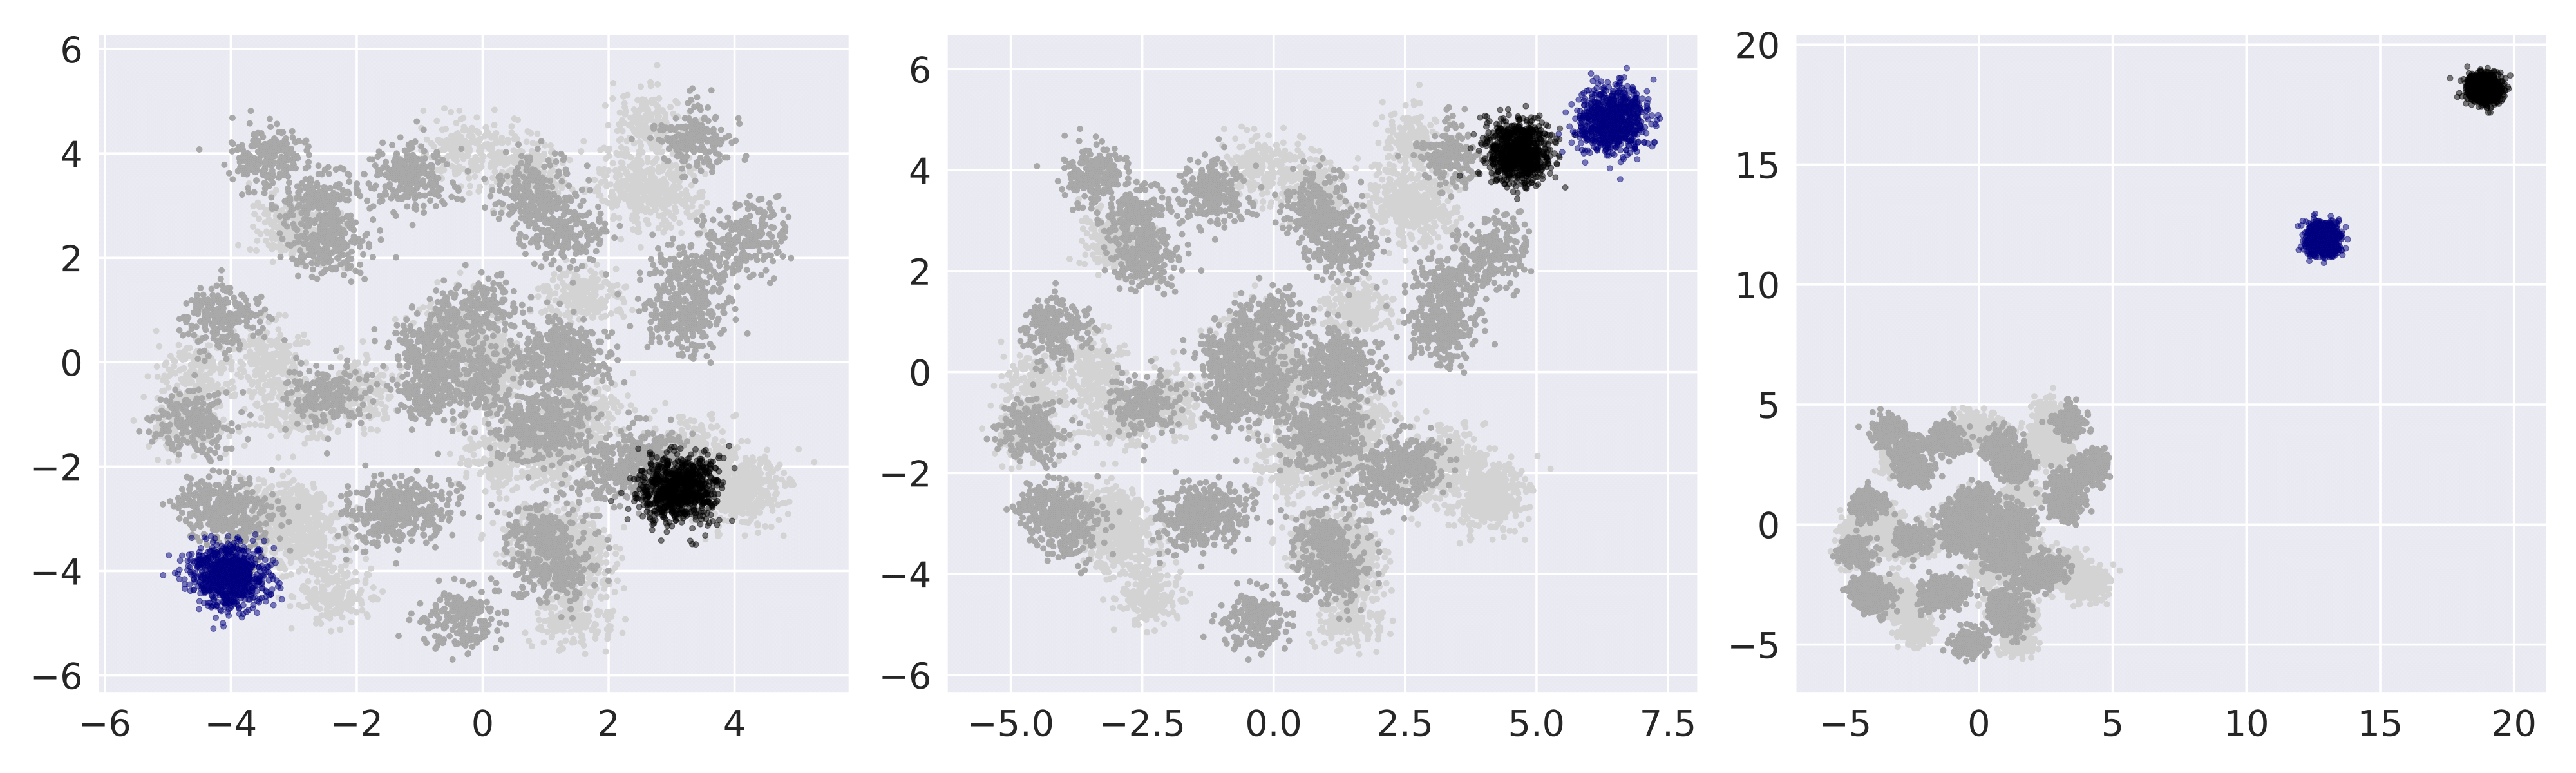
\includegraphics[ width=\linewidth]{images/chapter5/generalization_schemes.png}
\caption{Thirty mixtures drawn from the meta-distribution $\mathcal{M}$. We plot (in color) 3 unseen distributions whose parameters are drawn from (left) $U(-5, 5)$; (middle) $U(3,7)$; (right) $U(10, 20)$, the first two begin in and close to $\mathcal{M}$ whereas the last mixture is clearly outside of $\mathcal{M}$.}
\label{fig:mnist:gen}
\end{figure}

\section{Clustering Mixtures of Gaussians}
First, we present a simple clustering example to build intuition for meta-inference. Consider a standard VAE trained to capture a single mixture of two Gaussian (MoG) distributions $p_{\textup{data}}(x)$. Each component has isotropic covariance of $0.1$ and mean drawn from the uniform distribution, $U(-5, 5)$. The two components are mixed evenly and assigned a label of 0 or 1.
Then, inference $q_\phi(z|x)$ with  $z \in \{0, 1\}$ as a 1-D binary latent variable amounts to predicting which component $x$ belongs to, of which the true cluster label is recoverable up to a permutation.
Figure~\ref{fig:mnist:gen} shows a visualization of 30 mixtures from the meta-distribution. 

Given that an inference model $q_\phi(z|x)$ of a VAE can learn to cluster data from a \emph{specific} MoG, a meta-inference model $g_\phi(p_{\textup{data}_i},x)$ should correspond to \textit{a general-purpose clustering algorithm} that can separate out the components of any related, but previously  unseen mixture distribution $p_{\textup{data}_i}$. 
Concretely, we let each distribution $p_{\textup{data}_i} \sim p_\mathcal{M}$ be a MoG
% , where we represent each $p_{\textup{data}_i}(x)$ as a data set of samples $\mathcal{D}_i = \{x_1, ..., x_N\} \sim p_{\textup{data}_i}(x)$. 
% Thus, the meta-inference model $\hat{g}_\phi(\mathcal{D}_i, x)$ takes as input the data set as well as an observation $x \sim  p_{\textup{data}_i}(x)$.
and train a MetaVAE amortized over $N$ mixtures
% distributions from $p_{\mathcal{M}}$ 
to assess how well it can predict $z \in \{0,1\}$ for a given $x$ for an \emph{unseen test distribution}. 
% Like the VAE, meta-inference is equivalent to prediction. 
We measure this clustering accuracy on 1000 unseen but related MoGs 
sampled from the same meta-train distribution.
%with newly sampled component means from $U(-5, 5)$. 
While the VAE has a clustering error of $27.9$\% due to cases where there is extreme overlap in mixture components,
% \s{error seems way too high? might want to explain this}
the MetaVAE has an error of 9.9\% when $N = 50$. 
% \cc{Latter part of the sentence doesn't add much... 50 seems actually quite dense in the 2d space of possible configurations of means} 
% which is encouraging since 50 is a small number of the infinite possible mixture distributions in $\mathcal{M}$.
Moreover, larger $N$ improved the model's performance ($21.2$\% error with $N=10$ and $15.8$\% error with $N=20$) as expected. 
% which is sensible as the model sees more of the meta-distribution. 

\section{Inference for Classical Mechanics}

For a second demonstration, we consider an introductory problem in classical mechanics: objects sliding down inclined planes. Here, we are given a physics simulator that models a box that faces friction with the plane. 
% with the surface of a slope the box is set on. 
Each time the simulator runs, we see a new box with a different friction coefficient. The simulator then records the time it takes for the box to descend to the bottom of the plane. 
% Finally, say not all simulators are created equal, 
Each simulator has a different incline plane of length $L$ and incline angle $A$, and our task is to infer the coefficient of friction ($z$) from the observed descent time $(x)$ given a new simulator. 
\begin{figure}[h!]
\centering     %%% not \center
\includegraphics[width=0.9\linewidth]{images/chapter5/planes.pdf}
% \subfigure[]{\includegraphics[width=0.14\linewidth]{figures/physics/plane1.pdf}}
% \subfigure[]
% {\includegraphics[width=0.10\linewidth]{figures/physics/plane2.pdf}}
% \subfigure[]
% {\includegraphics[width=0.74\linewidth]{figures/physics/compiled.pdf}}
\caption{(a,b) Examples of planes with two lengths and angles. Mean squared error (MSE) between true and inferred friction for 304 simulators (lighter is better) using (c) MetaVAE and (d) VAE.}
\label{fig:physics}
\end{figure}
Building on \cite{le2016inference}, we tackle this problem with ``meta-compiled inference" and optimize: 
% \cc{good to write the \(p_{\theta^*_i}\) expectation in the \(\cdot \sim \cdot \) form for consistency}
% , where we optimize the following (see Appendix for derivation):
\begin{equation}
    \mathcal{L}_{\phi} = \mathbf{E}_{p_{\theta_i^*} \sim p_{\mathcal{M}}} \mathbf{E}_{x \sim p_{\theta_i^*}(x)}\left[-g_\phi(z| p_{\theta_i^*}, x) \right]
\end{equation}
The meta-distribution $\mathcal{M}$ represents all possible simulators of planes with $L \in [1,20]$ and $A \in [5,85]$ degrees, and $p_{\theta_i^*}(x, z)$ represents a fixed simulator. The marginal distribution, $p_{\theta_i^*}(x)$ is obtained by repeatedly simulating to build a data set $\mathcal{D}_i = \{ x \}$. Thus the empirical meta-inference model $\hat{g}_\phi(\mathcal{D}_i, x)$ takes the data set and the output of a single simulation $x$ as input. We amortize over 25 simulators with $L \in \{2,4,6,8,10\}$ and $A \in \{20,30,40,50,60\}$, and model $z$ as a continuous 1-D random variable (interpreted as friction). After training the MetaVAE, we measure the mean squared error between the true and inferred friction for unseen simulators from $\mathcal{M}$.
% We train a MetaVAE. Then, we freeze the encoder and docompiled inference for 300 generative models specified using lengths from 1 to 20 and angles from 5 to 80. We measure the MSE between inferred and true friction.
Despite seeing only 25 out of 304 simulators, the MetaVAE transfers well: we get less than 0.001 MSE for $A \in [20,70]$ and $L \in [2,20]$. A standard VAE trained on a single simulator ($L=10$, $A=45$) exhibits both much worse generalization performance and greater error overall (notice the scale in the legends). 
% \js{not sure if this is a fair comparison against VAE; what is specific here about the need of using VAE instead of a general probabilistic model to predict the coefficient?}

\section{Learning Distribution Statistics}
Next, we explore whether the MetaVAE is capable of "meta-learning" the concept of a sufficient statistic for exponential families~\cite{wainwright2008graphical}.
%random samples from several families of distributions. 
%In particular, we focus on the exponential family, as it is well known to encompass many common probability distributions \cite{wainwright2008graphical}.
% All distributions in the exponential family can be represented by a parameter (e.g. probability of success for a Bernoulli distribution). 
Given a set of random samples, a sufficient statistic is a function that maps this set to a vector in $\mathbb{R}^d$. For the exponential families, where each family member has the form \(p(x) \propto \exp (\theta \cdot \phi(x))\) for some parameter \(\theta\), this vector can be used to estimate the parameters of the distribution.
% For example, the sufficient statistic for realizations from a Gaussian random variable with fixed mean would return $x^2$, which is closely related to variance. 
In other words, the random samples (dataset) can be fully summarized by
% by the scalar value, and consequently 
the sufficient statistic, without any loss of information. 
% But more importantly, a data set of samples from one of these random vectors can be summarized by their sufficient statistics without any loss of information. 
% For example, the sample mean fully describes realizations of a Gaussian random variable with fixed variance. 
Now consider a \textit{vector} of random variables $(x_1, \cdots, x_k)$, each distributed i.i.d from the same distribution with sufficient statistic $\phi(x_i)$. 
%For exponential families, the sufficient statistic of the random vector
%from realizations of the random vector 
%is the sum $\sum_{i=1}^k \phi(x_i)$.
For exponential families, the sum $\sum_{i=1}^k \phi(x_i)$
is a sufficient statistic for the random vector. 
%from realizations of the random vector 
%of the scalar outputs of the sufficient statistic on realizations of each random variable in the vector 
%\mike{@stefano, is this true for Gaussian RVec?}
%. 
%As an example, a function of the sum of the number of successes given observations of a Bernoulli random vector is a sufficient statistic. 
As an example, the number of successes is a sufficient statistic for a vector of i.i.d. Bernoulli, and the sample mean and variance are for a vector of Gaussians. 
With this intuition, we ask the following: having seen many realizations of random vectors from different exponential family distributions, can we learn a sufficient statistic for %realizations of 
a new random vector that will be sufficient for estimating the parameters of its unseen, underlying distribution?
% sufficient statistic for realizations of a new random vector from an unseen distribution?
We aim to use the MetaVAE's meta-inference network to learn this mapping.
% to (meta) learn sufficient statistics -- that is, the MetaVAE should learn 
% to map a (sufficiently large) number of observations of random vectors distributed according to an exponential family to the sufficient statistic. 
%Precisely, if we fix the marginal distribution, then the meta inference model $g_\phi(\cdot, x)$, now a function of only $x$, is optimized to approximate the sufficient statistic where $x$ is a vector of random variables. We represent the marginal as a set of vectors of random variables, $\{x'\}$, each vector being distributed as $x$ is. Refer to the appendix for more exposition and details.
More precisely, the meta inference model $g_\phi(p_{\textup{data}_i},x)$ should act (as a function of $x$) as a sufficient statistic for an unseen distribution $p_{\textup{data}_i}$. 

\paragraph{Data and Model Setup}
We use 
% \cc{Only distributions named after people should be capitalised}
Gaussian (fixed variance), log-normal (fixed variance), exponential, symmetric beta, Laplace (fixed location), and Weibull (fixed scale) 
%random variables 
as exponential families. We then construct a set $\mathcal{M}_{\mathcal{I}}$ of 20-D 
vectors of random variables where each component is  i.i.d. distributed according to the same distribution. 
By construction, a random variable in this set will have only one free parameter, which can be found using the statistic learned by the meta-inference network.
We further restrict $\mathcal{M}_{\mathcal{I}}$ by bounding the free parameter to be within a range (e.g. Gaussians with mean between -5 and 5). 
After training, we measure how well we can infer the distributional parameters using the meta-inference model as a learned statistic for observations from unseen distributions. We compute the mean squared error (MSE) between the inferred and true parameters. 
% We refer the reader to the appendix for more details.

\begin{figure}
\centering     %%% not \center
\begin{subfigure}[b]{0.49\linewidth}
    \includegraphics[width=\linewidth]{images/chapter5/gaussian_only_test_set_mu.png}
\end{subfigure}
\begin{subfigure}[b]{0.49\linewidth}
    \includegraphics[width=\linewidth]{images/chapter5/gaussian_only_out_of_sample_set_mu.png}
\end{subfigure}
\begin{subfigure}[b]{0.49\linewidth}
    \includegraphics[width=\linewidth]{images/chapter5/lognormal_exapmle_good.png}
    \caption{Log Normal}
\end{subfigure}
\begin{subfigure}[b]{0.49\linewidth}
    \includegraphics[width=\linewidth]{images/chapter5/exponential_exapmle_good.png}
    \caption{Exponential}
\end{subfigure}
\caption{Colored circles represent 30 different $p_{\textup{data}_i} \sim p_{\mathcal{M}}$; black dots represent the inferred Gaussian means from the meta-inference model. (a) Test Gaussian distributions within $\mathcal{M}$; (b) Test distributions outside of $\mathcal{M}$. (c,d) Samples from the an unseen Log Normal or Exponential distribution $p_{\textup{data}_i} \in p_{\mathcal{M}}$ (red) and the true corresponding distribution defined by the inferred statistic (blue).}
\label{fig:gaussian_plot}
\end{figure}

\paragraph{Single Exponential Family}
Each $p_{\textup{data}_i}(x) \in \mathcal{M}$ is Gaussian with a mean sampled from $U(-5, 5)$.  At test time, we measure inference quality on (1) new random vectors from $\mathcal{M}$ whose entries are distributed as Gaussians with unseen means sampled from $U(-5, 5)$, and (2) a larger meta-distribution by sampling means from $U(-20, 20)$. We find the MetaVAE successfully learns the mean of the underlying Gaussians. Interestingly, in Figure~\ref{fig:gaussian_plot}(a), we find that the inference quality only decays near the boundary of the meta-distribution.
% For example, see the purple Gaussian near $(5, 5)$. In Figure~\ref{fig:gaussian_plot}(b), we also find that the meta-inference model is almost bounded within the $[5,5]$ square centered at the origin as it is unable to do inference for distributions outside of $\mathcal{M}$.
% \kristy{took out the sentence below, feel free to add back in}
% Finally, Figure~\ref{fig:gaussian_plot}(c) plots the MSE of the inferred statistic, enumerating over Gaussian distributions with means from $-10$ to $10$. 
We compare the MetaVAE to a VAE trained on one Gaussian distribution and find that doubly-amortizing increases the inference quality dramatically.
% \vspace{-1em}
%\paragraph{Log Normal and Exponential Marginals. } 
Then we move to two new exponential families: we similarly construct 30 log-normal random vectors with means from $U(-2, 2)$ and 30 Exponential random vectors with rates sampled from $U(0, 3)$. Like above, Figure~\ref{fig:explognorm_plot} shows good performance of meta-inference over $\mathcal{M}$ in each case.
\begin{figure}
\centering     %%% not \center
\begin{subfigure}[b]{0.34\linewidth}
    \includegraphics[width=\linewidth]{images/chapter5/gaussian_timeseries_plot.pdf}
    \caption{Gaussian}
\end{subfigure}
\begin{subfigure}[b]{0.31\linewidth}
    \includegraphics[width=\linewidth]{images/chapter5/lognormal_timeseries_plot.pdf}
    \caption{Log-Normal}
\end{subfigure}
\begin{subfigure}[b]{0.31\linewidth}
    \includegraphics[width=\linewidth]{images/chapter5/exponential_timeseries_plot.pdf}
    \caption{Exponential}
\end{subfigure}
\caption{(a) Mean squared error (MSE) between the true and inferred mean as the true mean of $p_{\textup{data}_i}$ spans $[-10, 10]$. The green region shows the  meta-distribution. 
% \cc{Say orange (dashed), blue (solid) etc}
The orange (dashed) line shows a singly-amortized VAE trained on a single $p_{\textup{data}_i}(x)$ with mean $[-1.2, 1.1]$ (randomly chosen) and the blue (solid) line shows the MetaVAE. 
% \cc{There is no d here} 
(b,c) show the MSE between the true and inferred parameters. The orange line is a singly-amortized VAE trained on a  randomly chosen distribution ($[-0.5, 1.8]$ for log-normal; $[1.4, 2.8]$ for exponential).}
\label{fig:explognorm_plot}
\end{figure}
% \noindent
% \vspace{-1em}
\paragraph{Many Exponential Families} 
Finally, we amortize over many types of distributional families simultaneously: we construct sets of 30 Gaussian, 30 log-normal, and 30 exponential random vectors (same bounds as above) to train a MetaVAE. This setup raises an interesting question: can we do inference for new random vectors comprised of \textit{unseen members of the exponential family} (e.g. Weibull)? 

We compare the performance a MetaVAE amortized over the 90 random vectors to 3 different (baseline) MetaVAEs, each of which is amortized over only 30 random vectors from one family (e.g. Gaussian). Below, Figure~\ref{fig:expfam_plot}(a-c) plot the MSE of inferred and true parameters for Gaussian, log-normal, and exponential (all of which are in $\mathcal{M}$). Due to the double-amortization gap, the best performing model is the MetaVAE amortized on random vectors only from that family. However, the 90-amortized MetaVAE only performs slightly worse, beating the remaining two baselines dramatically. Next, Figure~\ref{fig:expfam_plot}(d-f) show MSEs for three distributions not in $\mathcal{M}$: Weibull, Laplace, and Beta. The 90-amortized MetaVAE consistently outperforms all baselines. 
% This hints that amortizing inference over the exponential families together enables the model to learn more robust representations.

\begin{figure}[h]
\centering     %%% not \center
\begin{subfigure}[b]{0.9\linewidth}
    \includegraphics[width=\linewidth]{images/chapter5/legend.pdf}
\end{subfigure}
\begin{subfigure}[b]{0.32\linewidth}
    \includegraphics[width=\linewidth]{images/chapter5/mixed_gaussian_timeseries_plot.pdf}
    \caption{Gaussian}
\end{subfigure}
\begin{subfigure}[b]{0.32\linewidth}
    \includegraphics[width=\linewidth]{images/chapter5/mixed_lognormal_timeseries_plot.pdf}
    \caption{Log Normal}
\end{subfigure}
\begin{subfigure}[b]{0.32\linewidth}
    \includegraphics[width=\linewidth]{images/chapter5/mixed_exponential_timeseries_plot.pdf}
    \caption{Exponential}
\end{subfigure}
\begin{subfigure}[b]{0.32\linewidth}
    \includegraphics[width=\linewidth]{images/chapter5/beta.pdf}
    \caption{Beta($\alpha$, $\alpha$)}
\end{subfigure}
\begin{subfigure}[b]{0.32\linewidth}
    \includegraphics[width=\linewidth]{images/chapter5/weibull.pdf}
    \caption{Weibull(scale=1)}
\end{subfigure}
\begin{subfigure}[b]{0.32\linewidth}
    \includegraphics[width=\linewidth]{images/chapter5/laplace_scale.pdf}
    \caption{Laplace(loc=0)}
\end{subfigure}
\caption{Comparison of a MetaVAE amortized over three members of the exponential family to MetaVAEs amortized over only a single member. Each subplot shows an unseen distribution from either the meta-distribution (b,c,d) or another exponential family (e,f,g).}
\label{fig:expfam_plot}
\end{figure}

\section{Transformation-Invariance Experiments}
Imagine designing a scene understanding algorithm for a self-driving car. The video datasets used to train deep learning agents are typically collected in isolated settings, such as in large cities during favorable weather conditions.
% such as only at morning or night, or only in large cities. 
However, an agent deployed in the real world may face a variety of new settings such as paved roads in poorly-lit suburban areas.
% when deploying an algorithm in the real world, it may face all kinds of settings we have not seen beofre such as dusk or roads in small suburban communities. 
In such cases, we would hope the agent could abstract away unnecessary sources of variation, such as different lighting conditions, and act upon more salient characteristics in the scene (e.g. pedestrians) that it has seen previously during training. 
Inference in this scenario would mean learning representations that are "transferable," or invariant to nuisance transformations such as time of day.
% If we consider inference in this scenario, for a latent representation to be ``transferable", it must be invariant to different transformations that we deem irrelevant, such as time of day. 
We take a step towards this goal as 
% One of the benefits of meta-inference is learning a more transferable representation that can capture features representative all amortized distributions. To highlight this,
we study the MetaVAE for image distributions with explicit transformations, such as rotations or lighting. 
 
% \vspace{-1em}
We study MNIST \cite{lecun1998mnist} and NORB \cite{lecun2004learning}, where we amortize over three axes of variation each (e.g. a range of camera angles or background lighting). Further, we vary how different variations are split into meta-training and meta-test sets, summarized in Fig.~\ref{fig:splits}(a-c). For instance, we may train the MetaVAE only on images with bright backgrounds and evaluate on darker images. We consider three meta-splits: \textit{interleaved}, where every other value in the range of possible transformations is selected; \textit{sparse}, where half the number of values are chosen as in interleaved; \textit{contiguous}, where we split the range in two ``contiguous" halves and train only over the first half. Each meta-split is a different measure of transfer-ability. 
% We defer further details regarding dataset construction to the next section.
% \s{i feel that a digram showing the various meta datasets, meta test, etc pictorially would be very helpful (to put in appendix). showing digits grouped by rotation (say) and how they are used for train and test, labeling the $D_i$, $g$, etc}
% mw: i made a diagram

 \begin{figure}
    \centering
    \begin{subfigure}[b]{0.21\linewidth}
        \includegraphics[width=\linewidth]{images/chapter5/split_interleaved.png}
        \caption{Interleaved}
    \end{subfigure}
    \hspace{1em}
    \begin{subfigure}[b]{0.21\linewidth}
        \includegraphics[width=\linewidth]{images/chapter5/split_sparse.png}
        \caption{Sparse}
    \end{subfigure}
    \hspace{1em}
    \begin{subfigure}[b]{0.21\linewidth}
        \includegraphics[width=\linewidth]{images/chapter5/split_disjoint.png}
        \caption{Contiguous}
    \end{subfigure}
    \begin{subfigure}[b]{0.8\linewidth}
        \includegraphics[width=\linewidth]{images/chapter5/model_image.pdf}
        \caption{Meta-Inference Pipeline}
    \end{subfigure}
    \caption{(a-c) Three ways of defining the meta-training and meta-test splits; (b,c) pose a more difficult generalization challenge. (d) Overview of the doubly-amortized inference procedure. The meta-training set is used to train the MetaVAE (the test portion is to used to choose best parameters). The meta-test set is for evaluating the learned features, where the training portion is used to fit a linear classifier and the test portion is used to compute accuracy.}
    \label{fig:splits}
\end{figure}
 

% \vspace{-1em}
\paragraph{Evaluation Metric} We evaluate the latent representations on a downstream classification task. Having trained the empirical meta-inference model $\hat{g}_\phi(\mathcal{D}, x)$ using the meta-train set, we then embed observations from a distribution in the meta-test set. Each time we ``embed'' a test observation $x$, we feed in a data set $\mathcal{D}$ of samples \emph{from the meta-test set}. This way we construct a data set of latent features.

This feature set is split into a training and test subset. For both MNIST and NORB, each image has a corresponding label (e.g. digit or object class). 
% that we so far have not used. 
Using the training portion (darker red in Fig.~\ref{fig:splits}d) , we fit a logistic regression classifier on the representations to predict the labels and compute accuracy on the test subset (lighter red in Fig.~\ref{fig:splits}d). 
Critically, logistic regression seeks the best linear split between classes in the latent space. For it to achieve good accuracy, such a linear division must already exist.
% meaning that the information must be contained explicitly in the features. 
Thus, we treat a higher classification accuracy as a more transferable, invariant representation, as in \cite{berthelot2018understanding}.

\paragraph{Baselines} We compare the performance of MetaVAE against two baselines: the Neural Statistician (NS), a hierarchical VAE which models sets of observations with a global latent variable; and the Variational HomoEncoder (VHE), a more computationally-efficient variant of  NS. To ensure a fair comparison, we use the same hyperparameters and architectures across all models.

\begin{figure}
    \centering
    \includegraphics[width=0.9\textwidth]{images/chapter5/datasets_subset.png}
    \caption{Examples of interpolating across three transformations each for MNIST and Small NORB. Notice that for NORB (unlike MNIST), other transformations are not held constant as we vary an individual axis.}
    \label{fig:datasets}
\end{figure}

\paragraph{Transformed MNIST}

We artificially impose three axes of variations on MNIST digits. We transform each image with 18 \textit{rotations} (-180 to 180 by 20 degrees), 15 \textit{scales} (50\% to 200\% original size by 10\%), and  18 \textit{skews} (-180 to 180 by 20 degrees). 
% \cc{Is it worth disucssing the fact that flipping a 9 by 180 deg changes the label?}
See Fig.~\ref{fig:datasets}(a-c) for an example for a single digit. For each axes of variation, the other two are held constant e.g. skew and size are constant when varying rotation. 

% \vspace{-1em}
We find consistent evidence that MetaVAE features outperform both VHE and NS features across all settings, often by a significant margin. In particular, VHE and NS have decaying performance as scale increases to 2.0. Similarly, for extreme shear values near -80 and 80 degrees where the image is nearly flat (see Fig.~\ref{fig:datasets}c), VHE and NS again suffer greatly in performance.
% , understandably as these are aggressive shearing values. 
However, MetaVAE features transfer better: we do not notice a drop in accuracy as scale increases and the effect of significant shearing is more gradual. 
This suggests that MetaVAE has learned some invariances to transformations that NS and VHE lack.

\begin{figure}
    \centering
    \includegraphics[width=0.9\textwidth]{images/chapter5/results.pdf}
    \caption{Classification Accuracy on Transformed MNIST and Small NORB for three different splits: interleaved, sparse, and contiguous. Each subfigure shows the prediction accuracy on the test set of held out transformations --- gaps represent the values used in training the amortized generative model. We compare the performance of MetaVAE (black), the homoencoder (blue) and the statistician (red) and find appealing results for our proposed model.} 
    % \cc{I don't understand how it's possible to get over 80\% accuracy on 180 deg rotated MNIST if two of the classes (6 and 9) swap labels under transformation}}
    \label{fig:invariance:results}
\end{figure}

\paragraph{Small NORB}

The NORB dataset contains grayscale images of real world toys belonging to five classes: animals, humans, airplanes, trucks, and cars. The objects were imaged under 6 \textit{lighting} conditions, 9 \textit{elevations} (30 to 70 degrees every 5 degrees), and 18 \textit{azimuths} (0 to 340 every 20 degrees). Unlike the MNIST dataset, extraneous transformations are \textit{not} held constant as one transformation is varied. For example, as Fig.~\ref{fig:datasets}(f) shows, the azimuth and elevation (randomly) change as we vary lighting. This design, while more difficult to amortize, is more realistic in real world datasets where it is too expensive to collect data holding all other variables constant.

The MetaVAE representations outperform those of VHE and NS by 10 to 35\% accuracy. Overall, we notice accuracies are much lower in NORB than in MNIST, which is likely due to the complexity of learning real world image distributions and randomness from extraneous transformations. 
% Unlike MNIST, we no longer see VHE outperforming NS --- often the two accuracies are close to identical. 
We note that the strong performance of the MetaVAE despite varying transformations is promising support for our approach to meta-amortization, suggesting that the MetaVAE is able to ignore irrelevant signals while capturing the principal axes of variation.

\paragraph{Analysis}
We aim to quantitatively measure the intuition that amortizing over a family of transformations should yield representations that are invariant to that transformation.
% that transfer better to related perturbations across that axis of variation. 
% One of doing this is to we compare the effects of varying transformations on the learned representations.
% Next, we aim to quantitatively measure the effect of varying transformations on the learned representations.
% the intuition that ``varying transformations are being merged together." Specifically, we want to compare the learned embeddings as the transformation changes. 
For example, how much does the representation change as we alter the rotation in MNIST from -180 to 180, or interpolate the background from dark to light in NORB? 
To investigate, we use a MetaVAE amortized over a family of transformations (e.g. interleaved rotations) and compare the average
% \footnote{We average across a family of transformations (e.g. rotations of -180 to 180 by 20 degrees) and over images in the test set.} 
L$_2$ distance between the learned representation of a base (default) image and those of every rotated image. As a baseline, we compare this distance to the average L$_2$ distance of a separate family of transformations (e.g. scale) that this MetaVAE was not amortized over (e.g. having only seen different rotations during training). Table~\ref{table:distance} shows the distances for MNIST and NORB. Consistently, the lowest distances belong to the class of transformations that the MetaVAE was amortized over, which supports the intuition about learning invariances.

% \kristy{can't use tiny either :(}
\begin{table}[h]
\centering
% \tiny  
\begin{tabular}{r|c|c|c}
\toprule
Model Dataset & Rotation & Scale & Skew \\
\midrule
Rotated MNIST & $\mathbf{1.65}$ & $4.44$ & $4.09$ \\ 
Scaled MNIST &  $5.44$ & $\mathbf{2.16}$ & $4.92$ \\  
Skewed MNIST & $3.79$ & $4.89$ & $\mathbf{1.47}$ \\   
\toprule
Model Dataset & Elevation & Azimuth & Lighting \\
\midrule
NORB Elevation & $\mathbf{0.39}$ & $1.16$ & $1.27$ \\ 
NORB Azimuth &  $1.42$ & $\mathbf{0.44}$ & $1.26$ \\  
NORB Lighting & $1.69$ & $1.27$ & $\mathbf{0.26}$ \\
\bottomrule
\end{tabular}
\caption{L$_2$ distances between MetaVAE representations. Each row indicates the datasets  used for training; each column indicates the datasets used to compute representations post-training.}
\label{table:distance}
\end{table}

\section{Related work}
\paragraph{Rapid Adaptation through Meta-Learning.} Among the rich body of work on meta-learning \cite{vinyals2016matching,snell2017prototypical,gordon2018decision}, a common goal is to train models such that they will rapidly adapt to new, unseen classification tasks. Although the Neural Process (NP) \cite{garnelo2018neural,kim2019attentive} is similar to our work in that it derives predictions for new targets by conditioning the encoder network on a relevant \textit{context set}, it models uncertainty over a distribution of \textit{functions}.
Another line of research formulates proper initialization as the workhorse of successful meta-learning \cite{finn2017model,grant2018recasting}. Our meta-amortized inference procedure can be thought of as learning a good initialization for an inference model on a new target distribution. However, these approaches are not directly comparable because of their supervised nature. 

% \vspace{-1em}
\paragraph{Few-shot Generative Modeling.} This branch of research aims to train generative models such that they will generalize to unseen distributions at test time given only a few examples. The focus has been on few-shot density estimation, with approaches ranging from the use of
% attention \cite{rezende2016one}, 
conditioning \cite{bartunov2016fast} to nested optimization \cite{reed2017few}. Meta-inference however is not few-shot, and instead aims to learn transferable \textit{representations} for downstream tasks rather than density estimation alone.
% Although meta-inference aims to transfer to new distributions, it is not few-shot and instead prioritizes learning representations for downstream tasks rather than density estimation alone.
%that will generalize well to downstream tasks such as classification.

% \mike{it might be useful to write the losses for NS and VHE? that way we can accent the global variable more -- hard to understand what it is atm. also since we pushed all summary network stuff to the appendix, may not be worth mentioning here}
The most relevant prior works include the Neural Statistician \cite{edwards2016towards} (NS) and the Variational Homoencoder \cite{hewitt2018variational} (VHE), two very similar models that study inference over sets of observations. The VHE optimizes the following objective, 
% \cc{Can put \(x,\mathcal{D} \sim p_\mathcal{D}\) instead of two lines?}
% mw: we can take this out if we want it but i think its good to be explicit
\begin{equation}
    \mathbf{E}_{x,\mathcal{D} \sim p_{\textup{data}}}[\mathbf{E}_{z \sim q_\phi(c|\mathcal{D})}[\log p_\theta(x|c)] - \frac{1}{N}\textup{KL}(q_\phi(c|\mathcal{D}), p(c))]
    \label{eqn:homoencoder}
\end{equation}
where $\mathcal{D} = \{x_1, ..., x_N\}$ is a set of $N$ samples and $c$ is a global latent variable. 
% \cc{What is \(c\)?If it's just the same as \(z\), should just put it in as \(z\)}
We note that if we view $\mathcal{D}$ as an approximation for a marginal distribution, then NS and VHE also serve as baselines that can perform doubly-amortized inference. Like our proposed inference model $\hat{g}_\phi(\mathcal{D}, x)$, the distribution $q(c|\mathcal{D})$ in Equation~\ref{eqn:homoencoder} ingests a data set.
% cast the inference problem as learning a distribution over a \textit{set} of related distributions. 
However, both the VHE and NS utilize a global variable $c$ (isotropic Gaussian). 
% \cc{Ok, \(c\) is here. If possible, maybe try to rewrite this so the \(c\) isn't dangling for too long}
We believe this constraint is \textit{overly restrictive} in settings which require transferring to a diverse set of distributions, hurting generalization performance. Instead, the MetaVAE does not impose a distributional assumption, and we find that this non-parametric approach yields consistently better performance. 

\section{Conclusion}
In summary, we considered constructing an algorithm that can do inference for a  \textit{family} of probabilistic models. We introduced a meta-amortized inference paradigm and a new generative model, the MetaVAE. 
Through experiments on MNIST and Small NORB, we showed that the MetaVAE learned transferable representations that generalize well across similar data distributions in downstream tasks. 
% Through experiments on MNIST and Small NORB, we found good classification performance from the learned representations that suggests a notion of transformation invariance. 
Future work could consider new applications of meta-inference in video prediction \cite{ramanathan2015learning}.

\chapter{A Foundation Posterior}
\label{chapter:foundation}
Latent variable models are only one example in a rich class of graphical models used in practice. In this sense, the MetaELBO proposed in Section~\ref{chapter:metavae} is limited in applicability. However, the idea of twice-amortized inference can be more broadly used. In this next chapter, we will study a method based on masked language modeling to generate meta-amortized inference to larger class of probabilistic programs. 

\section{Preliminaries}

The primary goal of probabilistic programming is to enable practitioners from any domain to easily reason about random variables of interest \cite{gordon2014probabilistic,van2018introduction}.
The main challenge is to build posterior inference algorithms that are both efficient for practical usage and universal -- working for any program that might be written. Many probabilistic programming languages (PPLs) have been developed \cite{goodman2012church,minka2012infer,dippl,mansinghka2014venture,depaoli2016just,tolpin2016design,narayanan2016probabilistic,salvatier2016probabilistic,tran2016edward,carpenter2017stan,ge2018turing,cusumano2019gen,bingham2019pyro,tehrani2020bean} each with inference approaches with strengths and weaknesses. Some require users to assist in the inference process by programmatically specifying conditional independencies \cite{bingham2019pyro} or hand-crafting variational distributions \cite{ritchie2015controlling,bingham2019pyro,cusumano2019gen}. Others place strong restrictions on what kinds of programs can be represented \cite{carpenter2017stan}.
In this paper, we propose a complementary approach to scale inference for probabilistic programs. By treating a program as a constrained form of language with some additional nomenclature, we show that probabilistic inference can be viewed as masked language modeling \cite{vaswani2017attention,devlin2018bert}, a technique popular in natural language processing. Since little is assumed about the program, we need impose few constraints on users upfront. Further, the generality of treating inference as a text prediction problem naturally enables more advanced features, such as plating, with little additional work. We call this approach \textit{masked language inference}, or MLI.

While MLI can be used to solve inference queries for a single program, it becomes more powerful when \textit{meta-amortized} (or twice-amortized)  to do inference across different queries \textit{and} programs. Success requires a dense set of programs that cover sufficient diversity for the meta-algorithm to generalize. Since this is not always obtainable, we propose \textit{program augmentations} to enlarge a small dataset of programs. The result of meta-amortized MLI on the augmented programs is a \textit{foundation posterior}: a large neural network trained to do inference across many probabilistic programs. In experiments, we find the foundation posterior to be capable of both zero-shot inference and variational fine-tuning: given a program from the test set, we can achieve higher quality using the foundation posterior as an initial distribution. Indeed, fine-tuning the foundation posterior gives the best performance, for a wide range of runtimes, for a set of standard STAN programs.

% The rest of this paper is organized as follows. We provide some pertinent preliminaries in Section~\ref{sec:background}. In Section~\ref{sec:mli}, we describe MLI and show experiments for a variety of simple programs. In Sections~\ref{sec:meta} to \ref{sec:stan}, we apply MLI for meta-amortized inference, present our augmentation family, and construct the foundation posterior on the dataset of STAN programs. In Section~\ref{sec:related}, we relate our approach to prior work. Finally, in Section~\ref{sec:discussion}, we discuss limitations and future work.

\begin{figure}[tb]
    \centering
    \includegraphics[width=0.9\textwidth]{images/chapter6/overview.png}
    \caption{Masked language inference: treating a probabilistic program as a raw string, a large language model is trained to unmask latent variables conditioned on observed ones.}
    \label{fig:overview}
\end{figure}

\section{Background}
\label{sec:background}

% We briefly review some of the important technical concepts before introducing the method.

\paragraph{Probabilistic Programs}
We assume a class of probabilistic programs without loops and such that every line assigns a value to a variable. We note that all finite loops can be ``unrolled'' into a program without loops. Our constraint primarily disallows probabilistic programs with undecided runtime. Later, we relax this assumption to support loops over conditionally independent variables where unrolling may not be practical.
Variable assignment can take many different forms including sampling $x \sim \texttt{gaussian}(z, 1)$, direct assignment $x = z$, and function evaluation $x = \texttt{sqrt}(z)$. Importantly, we do not constrain what distributions and functions are allowed.

\paragraph{Approximate Inference} 
Let $p(x, z)$ be a joint distribution of latent variables $z$ and observed variables $x$. An inference query seeks to compute posterior beliefs $p(z|x) = \left(\frac{p(x,z)}{p(x)}\right)$ which is usually intractable as computing $p(x) = \int_z p(x,z) dz$ faithfully requires solving a difficult integral.
So, we settle for approximate techniques. Markov Chain Monte Carlo (MCMC) \cite{hastings1970monte,gelfand1990sampling} and variational inference (VI) \cite{jordan1999introduction,wainwright2008graphical,blei2017variational} are two widely used examples. Focusing on the latter, VI introduces a family of tractable distributions $\mathcal{Q}$ over the latent variables to find the member $q^* \in \mathcal{Q}$ that minimizes the Kullback-Leibler (KL) divergence between itself and the exact posterior $q^*(z) = \argmin_q \textup{KL}\left(q(z) || p(z|x)\right)$. Once found, $q^*$ serves as a proxy for the true posterior.
For probabilistic programs, $p(x,z)$ is easy to sample from (by simply executing the program) but difficult to score.
In these cases, we apply a useful trick by optimizing $\textup{KL}(p||q)$ rather than $\textup{KL}(q||p)$:
\begin{equation}
\mathcal{L}_{\textup{comp}}(\phi) = \mathbf{E}_{p(x)}\left[ \textup{KL}\left( p(z|x) || q_\phi(z|x) \right) \right] = \mathbf{E}_{p(x,z)} \left[-\log q_\phi(z|x) \right] + \textup{constant}
\label{eq:comp}
\end{equation}
Equation~\ref{eq:comp} is called compiled inference \cite{le2017inference}. Dropping the constant, the remaining expression is close to a supervised objective: choose the parameters of the distribution $q(z|x)$ that maximizes the likelihood of $(x,z) \sim p(x,z)$, samples from the probabilistic program.

\paragraph{Masked Language Modeling}
A seemingly unrelated technique is masked language modeling (MLM) \cite{devlin2018bert}, used widely by large language models like BERT \cite{devlin2018bert}. The MLM objective is a word prediction task \cite{taylor1953cloze}. Given an input sentence, each token has a probability of being replaced by a special mask token. The model then predicts the original token given the rest of the sentence.
In slightly more notation, let $x = (t_1, \ldots, t_{i-1}, \texttt{<mask>}, t_{i+1}, \ldots, t_n)$ be a sequence of tokens that form a sentence where the $i$-th token was randomly masked. The label is then just $y = t_i$. (This presentation assumes only one token is masked for simplicity whereas in general, multiple tokens can be masked in a single sentence.) Then, the MLM objective is written as $\mathcal{L}_{\textup{mlm}} = \mathbf{E}_{p(x)}\left[ \log p(y|x) \right]$ where $\log p(\cdot|\cdot)$ is cross entropy applied to softmax beliefs over the full vocabulary.

\section{Masked Language Inference}
\label{sec:mli}

We now connect approximate inference to MLM. Suppose we are given a single probabilistic program; we wish to do inference, but do not know apriori which variables in the program are observed and which are latent. During evaluation, an inquirer might hand you observations for any subset of the variables and present you with inference queries for the remaining unknown variables. To solve this challenge we aim to find a dataset of observed and latent assignments from which we can train a model to perform inference. We leverage the programitself to generate such a dataset. To do this, we edit the program slightly: For every line (which by design must be a variable assignment), we add an annotation with the value that the variable takes for a single execution of the statement. We do this with the syntax $\texttt{variable} = \texttt{expression} \rightarrow \texttt{value}$. For instance, $x \sim \texttt{gaussian}(0, 1) \rightarrow 0.132$.
% Note that this value may not be constant over repeated executions.
Unlike most prior PPLs, our program does not include an explicit \texttt{observe} statement. Rather the values annotated on the right side of each arrow is the observation for the variable in the statement.
Given a probabilistic program, execute it and annotate each line with assignments. Next, for each line, randomly mask the assignment with some probability. In other words, $x \sim \texttt{gaussian}(0, 1) \rightarrow \texttt{<mask>}$. Save this masked program and the true assignments for all masked variables as a single data point. To generate a dataset, we loop this procedure until we have a sufficiently large corpus.  Since the masking decision is made independently for each line, we can theoretically generate every possible permutation of observed and latent variables.

\subsubsection{Objective}

The dataset of programs as described is not far from a natural language corpus used by BERT. If we could use it to teach a model to unmask assignments of latent variables, then that is tantamount to inference. We formalize this intuition into a procedure we call \textit{masked language inference}, or MLI. See Fig.~\ref{fig:overview} for an overview.
The objective for MLI is a sum of two loss functions: one for traditional MLM and the other to score the true assignment for a latent variable under a posterior distribution parameterized by a neural network. In more detail, given a program $x = (t_1, \ldots t_n)$, we make two versions: for the first $x_{\textup{mlm}}$, we do what MLM typically does, choosing random tokens in the program string to mask; for the second, $x_{\textup{inf}}$, we do as described above and randomly mask assignments (the values to the right of the $\rightarrow$ symbol per line). Note that the two inputs $x_{\textup{mlm}}$ and $x_{\textup{inf}}$ have different tokens masked.

We use a transformer network $f_\theta: X \rightarrow \mathbf{R}^d$ that takes a raw string as input where $\theta$ are trainable parameters. We compute $v_{\textup{mlm}} = f_\theta(x_{\textup{mlm}})$ and $v_{\textup{inf}} = f_\theta(x_{\textup{inf}})$, both of which are a sequence of contextual vector embeddings $v = (v_1, \ldots v_n)$, one for each token. For each masked index $i$, we perform two actions, one for each input. For MLM, we have a classification head $g_\theta: \mathbf{R}^d \rightarrow |V|$ (e.g. a linear layer) that maps a vector $v_{\textup{mlm}}[i]$ to a probability for each token in the vocabulary $V$. For inference, we have an \textit{inference head} $h_\theta: \mathbf{R}^d \rightarrow \mathcal{Q}$ that maps a vector $v_{\textup{inf}}[i]$ to an approximate posterior distribution $q(t_i|x_{\text{inf}})$ in the family $\mathcal{Q}$ for the latent variable corresponding to token $t_i$.
For continuous variables, a common choice for $\mathcal{Q}$ is the Gaussian family, in which the network $h_\theta$ would return two vectors representing the mean and standard deviation. Alternatively, if the latent variable is binary, we might choose the family $\mathcal{Q}$ to be Bernoulli where $h_\theta$ returns a probability vector. The choice of distribution is flexible as long as scoring is differentiable (though sampling need not be).
% The choice of what distribution to use is left to the practitioner: if the chosen distribution is not the same as the true posterior (which may not have a closed form), then this is approximate inference. Unlike the motivational observation at the start of this section, this inference head is not unmasking a single value. Rather it is inferring the parameters of an approximating posterior, meaning we are not just doing maximum a posteriori.
In summary, the MLI objective is:
\begin{equation}
\mathcal{L}_{\textup{mli}}(\theta) = \mathbf{E}_{(x_{\textup{mlm}}, x_{\textup{inf}}) \sim p(x)}\left[ \log p(t_{\textup{mlm}} | x_{\textup{mlm}}) + \alpha \cdot \log p(t_{\textup{inf}} | x_{\textup{inf}}) \right]
\label{eq:mli}
\end{equation}
where $\alpha$ is a weight balancing the two losses, and $t_{\textup{mlm}}, t_{\textup{inf}}$ are masked tokens. While Equation~\ref{eq:mli} only masked a single token per loss, in practice we randomly mask 15\% of tokens in $x_{\textup{mlm}}$, and mask 15\% of assignments in $x_{\textup{inf}}$. This can be maximized with stochastic gradient descent.

\subsubsection{Empirical Analysis}
\label{sec:toyexpt}

To build intuition and demonstrate efficacy, we consider six probabilistic programs used in prior work \cite{che2021meta}. These programs implement popular models like Gaussian mixture models, hierarchical latent variable models, astronomical models, and incorporate library imports like the Rosenbrock function whose code is not specified in the program.
We recommend the reader refer to Section~\ref{sec:app:mli} for details. While these programs are simple, they specify wide prior distributions that result in high sample diversity over repeated executions, which should make the MLI task more challenging.

\begin{table}[t!]
\centering
\small
\begin{tabular}{lcccc}
\toprule
Program & \multicolumn{2}{c}{Test Set Evaluation} & \multicolumn{2}{c}{Ablation: No MLM} \\
& $\log p(z|x)$ & $\text{var}\left\{\log \frac{p(x,z)}{q(z|x)}\right\}$ & $\log p(z|x)$ & $\text{var}\left\{\log \frac{p(x,z)}{q(z|x)}\right\}$ \\
\midrule
Latent & $-1.538${\tiny$\pm 0.1$} & $1.895${\tiny$\pm 1.1$} &$-3.740${\tiny$\pm 0.2$} & $1.059$e$4${\tiny$\pm 91$} \\
Clustering & $-3.406${\tiny$\pm 0.4$} & $1.097${\tiny$\pm 0.6$} &  $-8.037${\tiny$\pm 3.1$} & $5.415$e$3${\tiny$\pm 5$e$3$} \\
Hierarchical & $-3.268${\tiny$\pm 0.1$} & $119.2${\tiny$\pm 60$} & $-7.088${\tiny$\pm 0.8$} & $5.162$e$9${\tiny$\pm 2$e$9$} \\
Multi-level & $-3.359${\tiny$\pm 0.5$} & $131.3${\tiny$\pm 31$} & $-8.363${\tiny$\pm 0.7$} & $3.219$e$8${\tiny$\pm 2$e$8$} \\
Milky way & $-2.896${\tiny$\pm 0.2$} & $66.09${\tiny$\pm 44$}& $-5.619${\tiny$\pm 0.2$} & $1.147$e$6${\tiny$\pm 1$e$6$} \\
Rosenbrock & $-1.827${\tiny$\pm 0.1$} & $6.673${\tiny$\pm 3.9$} & $-4.505${\tiny$\pm 0.1$} & $4.252$e$5${\tiny$\pm 2$e$5$} \\
\bottomrule
\end{tabular}
\caption{Masked Language Inference on a suite of  probabilistic programs. For each program, a test set is built using 1\,000 new executions with randomly masked assignments. We measure the average quality of inferring these masked values. We show averages over 3 runs.}
\label{tab:toy}
\end{table}

\paragraph{Evaluation Metrics}  We build a test set with 1,000 new executions of the program not used in training and randomly mask assignments. This set is held constant across runs and ablations. We evaluate performance with two metrics. First, we compute log probability of unmasked assignment under the approximate posterior specified by the model, averaged over all masked tokens per execution and all test executions. The larger this value is, the better the inference.

Second, we compute the variance of the log importance weights (IW), as in \cite{wu2018multimodal}. Since the approximate posterior $q$ acts as an importance distribution estimating the true posterior, we measure the quality by the variance of $\frac{p(x,z)}{q(z|x)}$, where lower variance is more desirable. If $q(z|x) = p(z|x)$, the importance weight would be a fixed constant, meaning zero variance.

%\begin{SCfigure}[h!]
\begin{figure}[h!]
  \centering
  \begin{subfigure}[b]{0.24\textwidth}
    \centering
    \includegraphics[width=0.45\textwidth]{images/chapter6/graph/indgauss.pdf}
    \caption{}
  \end{subfigure}
%  \hfill
  \begin{subfigure}[b]{0.24\textwidth}
    \centering
    \includegraphics[width=0.5\textwidth]{images/chapter6/graph/condind.pdf}
    \caption{}
  \end{subfigure}
%  \hfill
  \begin{subfigure}[b]{0.24\textwidth}
    \centering
    \includegraphics[width=0.5\textwidth]{images/chapter6/graph/expaway1.pdf}
    \caption{}
  \end{subfigure}
%  \hfill
  \begin{subfigure}[b]{0.24\textwidth}
    \centering
    \includegraphics[width=0.5\textwidth]{images/chapter6/graph/expaway2.pdf}
    \caption{}
  \end{subfigure}
\caption{Graphical model representations for the `Independent Gaussians' (a), `Conditional Independence' (b), and `Common Effect' (c,d) programs.}
\label{fig:graph}
\end{figure}

\paragraph{Results} Table~\ref{tab:toy} reports the performance on the six programs. We observe large probabilities (log close to 0) and small variance of log IW, which suggests good generalization of inference to new sample values. As a baseline, we include an ablation to MLI by removing the MLM term, which amounts to training the inference head only. We find smaller log probabilities (every log point is a significant difference) and much larger variance. Together, this suggests that the MLM term is important for generalization, likely as it helps the neural network understand program structure.
% That is, MLM regularizes the network to not overfit to memorizing the training examples.
For analysis on the distribution of variances, see Section~\ref{sec:app:mli}.

\subsection{Visualizing Attention Maps}

Prior works \cite{binder2016layer,voita2019analyzing,abnar2020quantifying,chefer2021transformer} using transformer networks in natural language have re-purposed the attention weights in the later layers as an mechanism to introspect model logic. In a similar vein, we leverage attention weights to approximate a dependency graph between random variables in the problem.

\paragraph{Datasets} We study simple probabilistic programs that exhibit independence and conditional independence between random variables. First, in Figure~\ref{fig:graph}(a), $z_1$ and $y_1$ are two independent Gaussian variables. We should expect independence between the sets $\{y_1, y_2\}$ and $\{z_1, z_2\}$. Second, in Figure~\ref{fig:graph}(b), we design a graphical model with a Bernoulli random variable $z$, and pick $a$ and $b$ using \texttt{if} statements to be conditionally independent given $z$. We add two Gaussian variables $x$ and $y$ that independently add noise around $a$ and $b$, i.e. $x \sim \mathcal{N}(a, 1)$. Finally, in Figure~\ref{fig:graph}(c,d), we create a common effect model with two potential causes: choose $x$ and $y$ to be independent Bernoulli variables, and set $z$ to be $1$ if $x \texttt{ or } y$ else $0$. We expect $p(x|z, y)$ to differ meaningfully from $p(x|z)$.
% Refer to Appendix for more details.
% For random variables with binary outcomes, we parameterize the inference head to output a single vector representing the weight of a Bernoulli distribution. Since we only need to score samples in the MLI objective (and not sample), this remains fully differentiable.

\begin{figure}[tbh]
  \centering
  \begin{subfigure}[b]{0.30\textwidth}
    \centering
    \includegraphics[width=\textwidth]{images/chapter6/heatmap/indgauss.pdf}
    \caption{}
  \end{subfigure}
  \hfill
  \begin{subfigure}[b]{0.30\textwidth}
    \centering
    \includegraphics[width=\textwidth]{images/chapter6/heatmap/condind.pdf}
    \caption{}
  \end{subfigure}
  \hfill
  \begin{subfigure}[b]{0.30\textwidth}
    \centering
    \includegraphics[width=\textwidth]{images/chapter6/heatmap/expaway.pdf}
    \caption{}
  \end{subfigure}
\caption{Heatmaps of attention norms for `Independent Gaussians', `Conditional Independence', and `Common Effect' programs. On the y axis, we show which variable has its assignment masked. On the x axis, we list all program variables. The brighter the color, the larger the weight.}
\label{fig:heatmap}
\end{figure}

\paragraph{Results} We report metrics similar to Table~\ref{tab:toy} for these programs in Section~\ref{sec:app:viz}. Here, we instead visualize attention: Suppose a single assignment in a program is masked. We first compute the L$_2$ norm over contextual vectors from the last layer for all tokens in the program. Next, we segment the norm sequence by program line, and compute the average norm per segment. Since each line is associated with a variable declaration, we can treat the average norm for a line as the ``attention'' the network is paying to this variable when inferring the masked variable. We hypothesize that this measure will be correlated to the dependency between the two variables.

Figure~\ref{fig:heatmap} shows the heatmap of attention norms for the three programs. For subplots (a) and (b), we mask each variable's assignment one at a time. The y-axis shows which variable is masked. In the `Independent Gaussians` program, the model approximates the independence between $\{z_1, z_2\}$ and $\{y_1, y_2\}$. For instance, in the first row of (a), when unmasking $y_1$, we see the network upweights the tokens corresponding to $y_1$ and $y_2$, but downweights the tokens for $z_1$ and $z_2$. The remaining rows show a consistent pattern. While it may seem peculiar at first for the model to pay attention to $y_1$ when unmasking $y_1$, we note that this is important for the model to understand what kind of variable $y_1$ is. Similarly, in the `Conditional Independence` program, the model approximates the independence between $\{a,x\}$ and $\{b, y\}$ given $z$. Looking at the first row, we see that unmasking $a$ focuses on variables $x$ and $z$ and downweights $b$ and $y$.
% We also highlight the last row: if we instead mask $z$, the model pays almost equal attention to all the other variables, with some emphasis on $a$ and $b$ as they are more directly related to $z$.
Finally, in subplot (c), the y-axis shows which variables are observed rather than which are masked, for clarity. The bottom row plots attention weights if we observe both $z$ and $y$ whereas in the top row, we only observe $z$. We see a stark contrast: in the bottom, the weights are roughly uniform; on top, the model gives little weight to $y$ to unmask $x$. 
% One interpretation is that observing $y$ (and $z$) determines the cause of the effect $z$. Thus, the network pays more attention to $y$ when observed. Without knowing $y$, the network can only rely on $z$.
% As the name of the program belies, this is reminiscent of the \textit{explaining away} phenomena, where observing a competing cause $y$ effects my belief of the current cause $x$ invoking the result $z$.

\section{Meta-Amortized Inference}
\label{sec:meta}

Rather than restrict to a single program, we wish to use MLI to do \textit{meta-amortized inference}, or zero-shot inference across programs.
% Interestingly, we note that the toy experiments in Section~\ref{sec:toyexpt} are already performing a simplified version of meta-amortization as the dataset is varying which variables are observed, not just the observation values. In this section, we study a more difficult variation:
Given a dataset of programs for training, how well can we do inference out-of-the-box for a new, unseen program? We assume this novel program is within the same meta-distribution as the training set of programs; otherwise the problem is unsolvable.

\subsection{Program Augmentations}

From prior work \cite{gordon2018meta,choi2019meta,che2021meta}, we know that the meta-training set must be crafted carefully for meta-amortized inference to perform well: the model must see enough programs that `span' the program space to be able to generalize to new programs from the meta-distribution. Collecting such a dataset for probabilistic programs is unfeasible. Instead, we propose a set of \textit{program augmentations}, inspired by data augmentations, to enlarge a small set of programs. The hope is that the larger dataset provides enough coverage to generalize to a new test program.
We propose the following augmentations, which can be recursively stacked on another:

\paragraph{Fuzz Function} Replaces a primitive function or distribution with a randomly sampled function or distribution. Replacements are constrained to have the same number of arguments as the original function. For example, the program $z = \texttt{rosenbrock}(a, b)$ might be augmented to $z \sim \mathcal{N}(a, b)$.

\paragraph{Fuzz Constant} Constants are replaced by newly sampled constants from known prior distributions. For example, $r \sim \mathcal{N}(0, 1)$ becomes $r \sim \mathcal{N}(0.1, 0.9)$.

\paragraph{Line Swaps} Swaps two independent program lines such that the dependency graph between random variables is unchanged. For example, a program with three lines $u \sim \mathcal{N}(0, 1); v \sim \mathcal{N}(1, 1); r = u + v$ could be augmented to $v \sim \mathcal{N}(1, 1); u \sim \mathcal{N}(0, 1); r = u + v$ but it would not be possible to swap the third line with any other given the dependency of $u$ and $v$ on $r$.

\paragraph{Cut and Glue} Replace the usage of a variable with another variable already defined in the program. Note that this augmentation changes the dependency graph. For example, $u = a + b; v = \texttt{sqrt}(u)$ could become $u = a + b; v = \texttt{sqrt}(b)$ where $b$ is defined earlier in the program.

\paragraph{Create and Use} Creates a new random variable and uses it in lieu of another variable or constant in the right-hand side of an expression. Note that this augmentation introduces a new random variable. For example, $u = a + b; v = \texttt{sqrt}(u)$ could become $u = a + b; r \sim \mathcal{N}(0, 1); v = \texttt{sqrt}(r)$.

Given that many of these augmentations meaningfully change the program by removing, editing or adding random variables, repeated applications of random augmentations can create novel programs in structure and content. In practice, not all augmentations when compounded result in legitimate programs. For instance, the augmentation $\texttt{rosenbrock}(1, -1) \rightarrow N(1, -1)$ by \textbf{fuzz function} is ill-defined. We perform rejection sampling and discard improper programs.

\subsubsection{Empirical Analysis}
\label{sec:toyexpt2}

To test program augmentations, we revisit the six  programs from Section~\ref{sec:toyexpt}. However, now we use five of them for meta-training, and hold out the ``Rosenbrock'' program for meta-test. We apply up to five random program augmentations to each program in both sets to create the training and test splits. Note that the test inputs are all derived from a novel program unseen by the model in training.
% We also note that the set of variables that are latent versus observed vary across augmentations of the same program.
This is a much more difficult generalization problem than prior experiments. As an important caveat, we assume knowledge of which external functions might be used. In the `Rosenbrock' program, we use the \texttt{rosenbrock} external function. We assume access to this when augmenting programs in the meta-training set such that \texttt{rosenbrock} may appear in training programs.
% While test programs can have novel structure and variables, they will not have novel functions.

\begin{table}[b!]
\centering
\small
\begin{tabular}{lcc}
\toprule
Model & \multicolumn{2}{c}{Test Set Evaluation} \\
& $\log p(z|x)$ & $\text{var}\left\{\log \frac{p(x,z)}{q(z|x)}\right\}$ \\
\midrule
MLI & $-8.160$ {\tiny $\pm 4.5$} & $15.10$ {\tiny $\pm 9.6$ } \\
MLI - Augmentations & $-246.6${\tiny $\pm 98$} & $355.9$ {\tiny $\pm 37$} \\
MLI + Finetuning & $-5.727$ {\tiny $\pm 4.0$} & $16.06$ {\tiny $\pm 7.2$} \\
Random + Finetuning & $-42.54$ {\tiny $\pm 89$} & $784.9$ {\tiny $\pm 242$}  \\
\bottomrule
\end{tabular}
\caption{Meta-Amortized Masked Language Inference over a suite of probabilistic programs. A test set of 1,000 programs are constructed using random augmentations on a held-out program.}
% Results are averaged over 3 runs. Two ablations measure the effect of augmentations and variational fine-tuning.}
\label{tab:toy:augment}
\end{table}

\paragraph{Results} We report results in Table~\ref{tab:toy:augment}. The top row shows the log likelihood and the variance of importance weights for MLI. The second row shows an ablation without augmentations (where we generate a dataset of equivalent size by re-executing programs as we did in Section~\ref{sec:toyexpt}). We observe a 100x improvement with augmentations, suggesting better generalization to unseen programs.

\section{Variational Finetuning}
\label{sec:finetune}

So far we have only studied ``zero-shot'' inference where an amortized inference model, given a new program, must do inference without any new computational expense. In more realistic scenarios, where test programs can look quite different than the training set, obtaining high quality inference in a zero-shot manner can be challenging. In this case, we propose to finetune our pretrained inference model using stochastic variational inference, or SVI \cite{hoffman2013stochastic,ranganath2014black,kucukelbir2017automatic}.

More specifically, fix a test program $x^*$ that we would like to do more high quality inference for. Suppose $x^*$ has $n$ observed data points $d_1, \ldots, d_n$, and $m$ latent variables we want to estimate $z_1, \ldots z_m$. Further, we are given $\hat{\theta}$, the parameters obtained from optimizing MLI on a pretraining dataset of programs. Since the composed functions $f \cdot h: X \rightarrow \mathcal{Q}$ map a probabilistic program to an approximate posterior, we define the shorthand $q_{\hat{\theta}}(z_{1:m}|d_{1:n}) = h(f(x^*))$.
% This notation is similar to description of the supervised regressor for amortized inference in Section~\ref{sec:background}.

We can optimize the evidence lower bound, which we recall is:
\begin{equation}
  \theta^* = \arg\max_{\theta \in \Theta} \mathcal{L}_{\textup{elbo}}(\theta) = \arg\max_{\theta \in \Theta} \mathbf{E}_{z_{1:m} \sim q_{\theta}(z_{1:m}|d_{1:n})} \left[\log \frac{p(d_{1:n}, z_{1:m})}{q_\theta(z_{1:m}|d_{1:n})}\right]
  \label{eq:elbo:finetune}
\end{equation}
Since we are not amortizing over programs in this finetuning step, Equation~\ref{eq:elbo:finetune} does not contain a second expectation over programs. That is, $z_{1:m}$, $d_{1:n}$ are the specific variables from $x^*$.
We initialize $\theta = \hat{\theta}$ to leverage pretrained weights. Note $p(\ldots)$ has no trainable parameters but acts as a likelihood scaling term for different values of $z_{1:m}$ and thus, cannot be dropped.

\paragraph{Results} In Table~\ref{tab:toy:augment}, we include an ablation  comparing the generalization of inference with and without fine-tuning. We fine-tune the inference network (from MLI pretraining), optimizing Equation~\ref{eq:elbo:finetune} separately for each program for 1,000 iterations. As a baseline, we also finetune the network from a random initialization. We observe that fine-tuning MLI further improves log probability by roughly 2 log points with comparable IW variance. On the other hand, fine-tuning from scratch results in poor performance, highlighting the importance of pretraining.

\subsection{Plating} In many applications of probabilistic inference, we have a dataset of observations that can be thousands of entries or more. We would like to make inference queries given all entries but naive unrolling is unscalable. 
%Transformers like BERT cannot handle arbitrarily long input sequences. 
Instead, we extend MLI to support `for' loops over conditionally independent variables. To do so, we will implement a form of \textit{minibatching} in our inference algorithm.

Figure~\ref{fig:plating} shows such a plating example. In the left program, we see 10 observations $d_1, \ldots, d_{10}$ such that $d_i \sim \texttt{gaussian}(x, 1)$ where $x$ is outside of the plate. But suppose 10 examples are too many to unroll. In the program on the right, we replace the `for' loop with a \texttt{plate(n)} token where the argument $n$ specifies the number of total iterations. Within the plate, we unroll two randomly subsampled iterations $i \in \{1, 4\}$. For multiple executions of this program, the iterations within the plate change, just like minibatching in neural network training. From the perspective of the transformer, this change does nothing more than add a new token to the vocabulary.

\begin{figure}[h!]
  \centering
  \includegraphics[width=0.5\textwidth]{images/chapter6/plating_process.png}
  \caption{Example of plating within MLI. There is a special \texttt{plate} token that specifies the total number of  observations, $n$. This defines a scope with a minibatch of $k \ll n$ observations.}
  \label{fig:plating}
\end{figure}

\paragraph{Why does this work?} Consider computing the program density $p(x, d_1, \ldots, d_n)$. This can be rewritten as $p(x)p(d_1, \ldots, d_n|x)$ of which the first term is a given. To compute the second term, observe that $d_1, \ldots, d_n$  are conditionally independent on $x$. So, $p(d_{1:n} | x) = \prod_{i=1}^n p(d_i | x)$. Now:
\begin{equation}
\log p(d_{1:n} | x) = \sum_{i=1}^n \log p(d_i|x) \approx \frac{n}{k} \sum_{j \in \textup{minibatch}} \log p(d_j|x)
\label{eq:minibatch}
\end{equation}
where the minibatch is of size $k \ll n$. We can make an unbiased (but higher variance) estimate of the full conditional distribution (and hence, the program density) using a small minibatch.
% This is a toy example but as long as the variables defined within the plate are independent over iterations, the program density can always be decomposed into a form akin to the one above.

% Given the minibatching trick in Equation~\ref{eq:minibatch}, we can compute $p(d_{1:n}, \{x\}) = p(d_{1:n} | x)p(x)$ where $p(x)$ is a known prior. Following this, we can optimize Equation~\ref{eq:elbo:finetune} to perform finetuning.
In the Appendix (Section~\ref{sec:app:irt}), we demonstrate plating on an item response theory (IRT) \cite{edgeworth1888statistics,hambleton1991fundamentals,rasch1993probabilistic,wu2020variational,wu2021modeling} model, a popular probabilistic program. In the next section, we will leverage plating use MLI on a bank of real world probabilistic programs with thousands of observations each.

\section{Foundation Posterior}
\label{sec:stan}

The relationship between MLI and variational fine-tuning is reminiscent of pretraining and downstream tasks, as popularized by self-supervised learning \cite{devlin2018bert,chen2020simple}. Inspired by foundation models \cite{bommasani2021opportunities}, we propose to frame the result of MLI as a \textit{foundation posterior} that can be finetuned downstream using SVI to perform inference for a wide array of probabilistic programs. The goal is to pay a large one-time cost in training a ``general'' inference model which may not be adequate for inference in all settings, but can be quickly adapted to new datasets with low cost.
To demonstrate the foundation posterior, we meta-amortize inference over a set of standard Stan \cite{carpenter2017stan} programs from PosteriorDB \cite{magnusson2021}, a benchmark dataset for evaluating  inference algorithms \cite{baudart2021compiling,baudart2021automatic,yao2020stacking,zhang2021pathfinder,durr2022bernstein}.
% PosteriorDB contains 49 programs in the Stan language, which we manually convert to the notation presented in the paper.

\paragraph{Setup} We hold out three programs from PosterioDB for evaluation, and optimize the foundation posterior on the remaining set. (Programs containing HMMs were removed as we are currently unable to support that graph structure.) Plating with minibatches of size 5 is used for all programs to fit observations within the transformer's 512 token limit. After pretraining, we optimize Equation~\ref{eq:minibatch} for each test program individually, varying the number of steps of fine-tuning across 0 (zero-shot), 10, 100, and 1000. As baselines, we use \texttt{CmdStanPy} to run Stan-native NUTS and ADVI. For NUTS, we vary the number of mixing steps between 10 and 10k; for ADVI we vary the number of iterations between 100 and 1M. Each program comes with 10k pre-computed posterior samples fit using long runs of expert-tuned NUTS in Stan, constituting the gold standard. To evaluate inference quality we draw 10k samples and perform a hypothesis test between the gold and drawn samples. If the p-value is high, we conclude the two sets of samples are likely from the same distribution.

\begin{figure}[h!]
  \centering
  \begin{subfigure}[b]{0.32\textwidth}
    \centering
    \includegraphics[width=\textwidth]{images/chapter6/stan/earnings_logearn_height.pdf}
    \caption{Earnings}
  \end{subfigure}
  \hfill
  \begin{subfigure}[b]{0.32\textwidth}
    \centering
    \includegraphics[width=\textwidth]{images/chapter6/stan/kidiq_kidscore_interaction.pdf}
    \caption{KidIQ}
  \end{subfigure}
  \hfill
  \begin{subfigure}[b]{0.32\textwidth}
    \centering
    \includegraphics[width=\textwidth]{images/chapter6/stan/nes1976_nes.pdf}
    \caption{NES1976}
  \end{subfigure}
\caption{Comparisons of MLI to native inference methods in the Stan programming language, such as NUTS or ADVI. For any inference algorithm, we draw samples from the posterior and compute similarity to ground-truth posterior samples through a Kolmogorov-Smirnov test.}
\label{fig:stan}
\end{figure}

\paragraph{Results} Figure~\ref{fig:stan} reports results on held-out Stan programs. We plot the cost of inference computation (wall-clock time) on the x-axis in log-seconds. For MLI, we sum the cost of fine-tuning and the cost of forward passes to sample. For NUTS and ADVI, we ignore the cost of compilation, measuring mixing time and optimization time, respectively.
On the y-axis, we plot the p-value.
A better inference algorithm would bias towards the top left corner, achieving a higher p-value at lower cost. Each point in the plot represents a setting -- we redo inference with different finetuning steps or mixing steps, etc. Each line groups together a single inference algorithm.

First, observe that ADVI in Stan performs poorly (p-value < 0.5) despite being cheap. In the KidIQ program, it is unable to surpass a p-value of 0, suggesting poor posterior samples. Second, we see that NUTS is computationally expensive but converges to a p-value of 1 in all cases, as expected since the gold samples are derived from NUTS. We observe foundation posterior to achieve a compromise between the two: it is cheaper than HMC but achieves higher inference quality than ADVI in Stan. The left-most point in the MLI curve represents zero-shot inference, which we find comparable to ADVI despite the latter training for up to 1M steps. Finally, the gray line shows an additional baseline where we finetune a transformer from scratch. We observe that initializing from a foundation posterior is critical to good inference.
 % as finetuning from scratch results in p-value 0.

\section{Related Work}
\label{sec:related}

% There is a rich history of literature improving  posterior inference algorithms like MCMC or HMC, such as learning proposal distributions \cite{andrieu2008tutorial} or more efficient hyperparameter tuning \cite{hoffman2014no}. We view our approach as an orthogonal contribution that can be used together with these approaches. For instance, future work could explore using foundation posteriors as proposals for faster convergence in MCMC and HMC mixing. In this paper, we focus more on stochastic variational inference \cite{jordan1999introduction,ranganath2014black} that rely on neural networks to define approximate inference distributions, which we discuss next.

\paragraph{Amortized Inference} Traditionally, an inference query $q(z)$ is solved for a single assignment of the observed variable $x$. However, in many applications, we may be interested in solving the same inference query for many observations $x_1, x_2, \ldots, x_n$. Re-solving the same inference query from scratch for all $n$ related queries seems wasteful. Amortized inference \cite{gershman2014amortized,stuhlmuller2013learning} was proposed as a more efficient alternative by learning a function $q(z|x)$ that maps a observed assignment $x$ to a distribution over the latent variable $z$. In doing so, we ``amortize'' the cost of inference with a large one-time cost in defining $q$, after which an inference query can be solved with a single function application. Without amortization, the foundation posterior would not be a very efficient inference algorithm.

% \textbf{Compiled Inference}$\quad$ In some applications, we may be given a generative model that we need not learn from data. For instance, a probabilistic program specifies a hand-written generative model: executing the model forward maps latents to observations. In these cases, we can optimize a reduction of the evidence lower bound \cite{kingma2013auto,rezende2014stochastic}: the likelihood term drops from the expression, leaving a supervised objective matching latents to observations. This algorithm is called ``compiled'' inference \cite{le2017inference}. We note that masked language inference is a special case of compiled inference.
% In our experiments, we measure the benefit of meta-amortized inference with compiled inference as a baseline.

\paragraph{Meta-Inference} Meta-learning has been used to do inference amortized over both queries and a family of generative models \cite{choi2019meta,gordon2018meta,iakovleva2020meta}. These works have shown that ``meta-amortized'' inference can generalize well within the family of models it was trained on, even members not explicitly seen in training. The foundation posterior is a meta-amortized algorithm trained with masked language inference. Unlike prior works, we not only evaluate zero-shot inference but also the ability to serve as an effective starting point for further fine-tuning.

\begin{figure}[h!]
  % \begin{subfigure}[b]{0.49\linewidth}
  %   \begin{center}
  %     \includegraphics[width=0.9\linewidth]{mh/accept.pdf}
  %   \end{center}
  % \end{subfigure}
  \begin{center}
  \includegraphics[width=0.7\linewidth]{images/chapter6/mh/rhat.pdf}
  \end{center}
  \caption{Distribution of R-hat scores over 100 executions of the `Latent' program when using the approximate posterior (red) versus the prior (orange). Averages are the dotted lines.}
  \label{fig:mh:accept}
\end{figure}

Most relevant to our work is a meta-learning approach \cite{che2021meta} that builds a white-box inference algorithm by matching every step in a probabilistic program with neural network whose role is to ``invert'' it. Foundation posteriors trade explainability for flexibility. Our approach is not white-box: inference is performed by a single black box neural network. In return, our approach assumes no structure: it treats the program as nothing more than a  string, making its generalization capacity greater than the approach in \cite{che2021meta}. We view these two methods as optimizing for distinct properties.

\paragraph{Foundation Models} Foundation models \cite{bommasani2021opportunities} are a blanket term for large unsupervised models that map data to representations. Examples include ResNet \cite{he2016deep} in computer vision, BERT \cite{devlin2018bert} and GPT \cite{brown2020language,radford2019language} in natural language, Wav2Vec \cite{schneider2019wav2vec,baevski2020wav2vec} in speech, and CLIP \cite{radford2021learning} and Data2Vec \cite{baevski2022data2vec} in multimodal applications. Foundation models are treated as frozen backbones whereupon a small portion is finetuned  for a downstream task. Our motivation for the foundation posterior is precisely this: learn a good posterior ``initialization'' that can be quickly finetuned for  downstream inference.

\section{Discussion}
\label{sec:discussion}

% We discuss important limitations, summarize findings, and present future directions for research.

\paragraph{Limitations} First, optimizing  transformer networks is computationally costly, requiring accelerated hardware. For practitioners simply interested in a small set of inference queries, it is simpler to use MCMC or VI. Second, MLI as described is not sufficient for all programs: in PosteriorDB, classes of graphical models like HMMs are difficult to represent as text. Third, our approach, being reliant on deep learning, is limited in its explainability. In the case that inference fails, we are unable to reason about the root cause. Finally, the success of foundation models \cite{bommasani2021opportunities} is largely predicated on large datasets with millions of entries. Unfortunately, we do not know of any large collections of probabilistic programs other than PosteriorDB, which in comparison, is of modest scale.
% We would expect a foundation posterior optimized thousands to millions of programs would potentially be quite general.
% Future work could compile such a dataset.
% Almost all of the experiments presented assume continuous random variables, meaning we could model posteriors using Gaussian distributions. However, since MLI does not require sampling, we are not restricted to posterior families that are reparameterizable \cite{kingma2013auto,rezende2014stochastic}. For instance, like we did in Section~\ref{sec:app:viz}, we can specify discrete posteriors (e.g. Bernoulli or Categorical) for discrete random variables with finite support.

\paragraph{Future Work} Future work could investigate foundation posteriors that act as proposal distributions for MCMC-based methods.
% Moreover, as Bayesian networks are a subclass of probabilistic programs, future research could study applying foundation posteriors to BayesNet challenges.
As a first step, we run Metropolis Hastings on one of the six toy programs, and compute R-hat \cite{gelman1992inference}. We achieve a score of $1.011$ ($\pm 0.009$ over 100 test programs) when using the foundation posterior as the proposal compared to $1.043$ ($\pm 0.059$) when using the prior distribution. Best practice deems a chain sufficiently mixed if R-hat is less than $1.05$. More analysis is needed to better understand the efficacy of foundation posteriors in this context.

\paragraph{Summary} We proposed a meta-amortized inference algorithm for probabilistic programs using masked language modeling. With this algorithm, we build a foundation posterior capable of fast zero-shot inference that can also be finetuned for more accuracy.
We are optimistic that the generality of the approach, despite its computational burden, can make for practical and scalable inference.


\part{Real World Applications}

\chapter{Item Response Theory}
\label{chapter:vibo}
We transition from presenting inference algorithms to applying them in practice. In the following chapter, we frame measuring student ability as an inference challenge, and leverage many of the same tools from previous chapters to handle the complexity of real world student cognition.

\section{Preliminaries}
\label{sec:introduction}

The task of estimating human ability from stochastic responses to a series of questions has been studied since the 1880's \cite{edgeworth1888statistics}
%%bd goes back way further! see, for example, Stable URL: http://www.jstor.org/stable/2339898
%%mw fixed
in thousands of papers spanning several fields.
The standard statistical model for this problem, Item Response Theory (IRT), is used every day around the world, in many critical contexts including college admissions tests, school-system assessment, survey analysis, popular questionnaires, and medical diagnosis.
As datasets become larger, new challenges and opportunities for improving IRT models present themselves.
On the one hand, massive datasets offer the opportunity to better understand human behavior by fitting more expressive models.
On the other hand, the algorithms that work for fitting small datasets often become intractable for larger data sizes.
% Indeed, despite a large body of literature, contemporary IRT methods fall short -- it remains surprisingly difficult to estimate human ability from stochastic responses. 
%%bd says who? i am not just being a pedant but am not entirely sure what we mean. i think most psychometrics people would say that merely getting estimates isnt that big of a challenge at this stage. i would suggest we try to refine to more clealry indicate the problem we care about. to my mind, that is a typical reliance on highly parametric models required to do inference given the latent variables (ie ability) that make estimation complex here.
%% mw: @ben, this is a good point! I am going to focus this paragraph on just the scalability argument and bring up this parametric argument later for the deep generative IRT parts
One crucial bottleneck is that the most accurate, state-of-the-art Bayesian inference algorithms are prohibitively slow, while faster algorithms (such as the popular maximum marginal likelihood estimators) sacrifice accuracy with simplifying assumptions and poorly capture uncertainty.
This leaves practitioners with a choice: either have nuanced Bayesian models with appropriate inference or have timely computation.

In the field of artificial intelligence, a revolution in deep generative models via \emph{variational inference} \cite{kingma2013auto,rezende2014stochastic} has demonstrated an impressive ability to perform fast inference for complex Bayesian models.
In this paper, we present a novel application of variational inference to IRT, validate the resulting algorithms with synthetic datasets, and apply them to real world datasets.
We then show that this inference approach allows us to extend classic IRT response models with deep neural network components. We find that these more flexible models better fit large real world datasets.
Specifically, our contributions are as follows:

\begin{enumerate}
    \item \textbf{Variational inference for IRT:} We derive a new optimization objective --- the Variational Item response theory Lower Bound, or VIBO --- to perform inference in IRT models.
    By learning a mapping from responses to posterior distributions over ability and items, VIBO is 
    trained to efficiently solve many inference queries at once; a process called \textit{amortization}.
    %bd this word is a mystery to me. can we parenthetically help reader here?
    %mw: great point. is this better?
    \item \textbf{Faster inference:}
    We find VIBO to be much faster than previous Bayesian techniques and usable on much larger datasets without loss in accuracy.
    \item \textbf{More expressive:} Our inference approach is naturally compatible with deep generative models: we train neural networks to learn a joint mapping from student ability and item characteristics to response probabilities. As universal function approximators, neural networks capture nonlinear mappings that are more flexible than commonly used parametric IRT models (e.g. 2PL or LPE).
    % and, thus, we extend Bayesian IRT models to use neural-network-based representations for inputs, predictions, and student ability. 
    %%bd i'm not clear on what inputs and predictsion mean in this context
    %% mw: fixed.
    To the best of our knowledge, we are the first to apply deep generative models to IRT. %%bd i am always hesitant to include claims of primacy as they basically serve as a dare for some wacky reviewer to prove you wrong. but, if you're sure it's right... :)
    %% mw: i want to be a little bold here and try to claim this contribution. We can retract if we get a lot of pushback!
    % \item \textbf{Simple code:} We open-sourced both a Python pip package (TODO) and a CRAN R package (TODO), inspired by MIRT, to make VIBO accessible for practitioners.
    We leverage this flexibility to uncover asymmetric item characteristic curves from data alone, and show examples on the TIMSS dataset.
    \item \textbf{Real world application: } We demonstrate the impact of faster inference and expressive models by applying our algorithms to datasets of responses from PISA, DuoLingo and Gradescope. We achieve up to 200 times speedup relative to conventional parametric approaches and show improved accuracy at imputing hidden responses.
    At scale, these improvements in efficiency save hundreds of hours of computation.
    % \item \textbf{Learning item characteric curves:} We show how to use VIBO to uncover asymmetric item characteristic curves from data alone---an example motivated by recent work in the psychometrics literature---and show examples using the TIMSS dataset. \ndg{this should really be part of point 3 -- we extend the generative model first in constrained ways, such as learning the characteristic curves, and then by replacing the classical generative model with a deep network.}
\end{enumerate}

As a roadmap, in the following sections, we first describe the item response theory challenge before we present the main algorithm. Then, through experiments on several measurement datasets, we show its impact on speed and accuracy.
We discuss several extension to the IRT generative model, made possible by the VIBO algorithm: handling polytomous responses, capturing asymmetric item characteristic curves, and using flexible deep generative models. We close with limitations and broader impact of the proposed method.
% The potential impact of this work is two-fold: More accurate models can be constructed for existing applications of Item Response Theory, such as for visual acuity tests (Piech, 2019), large scale language studies (Hartshorne, 2018), or educational assessments such as PISA (Organisation, 2016).

\section{Preliminaries}
\label{sec:background}

We briefly review several variations of IRT and the fundamental principles of approximate Bayesian inference, focusing on stochastic variational inference.
A visualization of the different item response functions discussed can be found in Figure~\ref{fig:icc}.
%%bd suggest we add: We discuss several item response models; a visualization of the item response functions invoked by these models can be found in Figure X.

\begin{figure}
    \centering
    \includegraphics[width=0.6\textwidth]{images/chapter7/icc.pdf}
    \caption{Item characteric curves (ICC) for various IRT models. IDL represents an ideal point model (non-monotonic); LPE represents a logistic positive exponent model (asymmetric). For 3PL, we set the guess parameter $g_j = 0.3$. For LPE, we vary $b_j = 0.3$ and $b_j = 3.0$.}
    \label{fig:icc}
\end{figure}

% Imagine answering a series of multiple choice questions.
% For example, consider a personality survey, a homework assignment, or a school entrance examination.
% Selecting a response to each question is an interaction between your ``ability'' (knowledge or features) and the characteristics of the question, such as its difficulty.
% The goal in examination analysis is to gauge this unknown ability of each student and the unknown item characteristics based only on responses.
% Early procedures (Edgeworth, 1888) defaulted to very simple methods, such as counting the number of correct responses, which ignore differences in question quality.
% In reality, we understand that not all questions are created equal: some may be hard to understand while others may test more difficult concepts.
% To capture these nuances, Item Response Theory (IRT) was developed as a mathematical framework to reason jointly about people's ability and the items themselves.

% The IRT model plays an impactful role in many large institutions.
% It is the preferred method for estimating ability in several state assessments in the United States, for international assessments gauging educational competency across countries (Harlen, 2001), and for the National Assessment of Educational Programs (NAEP), a large-scale measurement of literacy and reading comprehension in the US (Ravitch, 1995).
% Beyond education, IRT is widely used in cognitive science and psychology, for instance, to study  language acquisition and development (Hartshorne, 2018; Magdalena, 2016; Frank, 2017; Braginsky, 2015).
Item response theory (IRT) is widely used to model the probability of a correct response conditional on a latent set of ``abilities'' and item characteristics, with applications in educational assessment \cite{edgeworth1888statistics,ravitch1995national,harlen2001assessment}, language development \cite{braginsky2015developmental,luniewska2016ratings,frank2017wordbank,hartshorne2018critical}, and many other areas.

\begin{figure}
    \centering
    \begin{subfigure}[b]{0.3\textwidth}
        \centering
        \includegraphics[width=0.75\textwidth]{images/chapter7/irt_1pl.pdf}
        \caption{}
    \end{subfigure}
    \begin{subfigure}[b]{0.3\textwidth}
        \centering
        \includegraphics[width=0.75\textwidth]{images/chapter7/irt_2pl.pdf}
        \caption{}
    \end{subfigure}
    \begin{subfigure}[b]{0.3\textwidth}
        \centering
        \includegraphics[width=0.75\textwidth]{images/chapter7/irt_3pl.pdf}
        \caption{}
    \end{subfigure}
    \caption{Graphical models for the (a) 1PL, (b) 2PL, and (c) 3PL Item Response Theories. Observed variables are shaded. Arrows represent dependency between random variables and each rectangle represents a plate (i.e.~repeated observations).}
    \label{fig:irt_graph}
\end{figure}

%%bd i think we could probably delete the stuff in the section ahead of this as it should be highly familiar to journal's readership. we could add a first sentence saying ``IRT is widely used to model the probability of a response conditional on some latent set of ``abilities'' (then add cites)''
%%mw: done.
IRT has taken many forms over it's rich history. As review, we begin with the most standard (see Figure~\ref{fig:irt_graph}).
The simplest class of IRT summarizes the ability of a person with a single parameter.
This class contains three versions: 1PL, 2PL, and 3PL -IRT, each of which differ by the number of free variables used to characterize an item.
The 1PL-IRT model, also called the Rasch model \cite{rasch1960studies}, is given in Equation~\ref{eq:1pl_irt},
\begin{equation}
    p(r_{i,j}=1|a_i,d_j) = \frac{1}{1 + e^{-a_i - d_j}}
\label{eq:1pl_irt}
\end{equation}
where $r_{i,j}$ is the response by the $i$-th person to the $j$-th item.
There are $N$ people and $M$ items in total.
Each item in the 1PL model is characterized by a single number representing difficulty, $d_j$.
%%As the 1PL model is equivalent to a logistic function, a higher difficulty requires a higher ability in order to respond correctly.
The 2PL-IRT model adds a \textit{discrimination} parameter, $k_j$ for each item that controls the slope (or scale) of the item response function. 
%%bd if you accept edit above re the logistic function line, i think you could just talk about k_j controlling slope of resulting item response function. in fact, it might be useful to introduce the item response function as the key thing we're focusing on here (eg when we say 'accuracy' we mean accurate estimation of that function)
%% mw: changed logistic -> item response function. Will try to mention item response functions in the evaluation section. I think too early to mention here.
Items with higher discrimination to more quickly separate people of low and high ability.
The 3PL-IRT model further adds a \textit{pseudo-guessing} parameter, $g_j$ for each item that sets the asymptotic minimum of the item response function.
We can interpret pseudo-guessing as the probability of success if the respondent were to make a (reasonable) guess on an item.
The 2PL and 3PL -IRT models, respectively, are:
\begin{equation}
   p(r_{i,j}|a_i, k_j, d_j) = \frac{1}{1 + e^{-k_j a_i - d_j}} \textup{ or } p(r_{i,j} | a_i, g_j, k_j, d_j) = g_j + \frac{1 - g_j}{1 + e^{-k_j a_i - d_j}}
\label{eq:2and3pl_irt}
\end{equation}
See Figure~\ref{fig:irt_graph} for graphical models of each of these IRT models where arrows represent conditional dependencies. 
% `Below, we may write $\textbf{d}_j = \{k_j, d_j\}$ or $\textbf{d}_j = \{g_j, k_j, d_j\}$ to represent the set of item characteristics. 

\subsubsection{Multidimensional Extensions}

While ability and item characteristics presented above are scalars, later extensions proposed more flexible IRT models using multi-dimensional representations of ability and item discrimination \cite{ackerman1994using,mcdonald2000basis,reckase2009multidimensional}.
However, in return for flexibility, multi-dimensional IRT (or MIRT) is computationally cumbersome, requiring expensive numerical quadratures \cite{liu1994note,naylor1982applications} or MCMC sampling \cite{houts2015flexmirt}  to perform inference. 
% A single ability dimension is sometimes insufficient to capture the relevant variation in human responses.
% For instance, if we are measuring a person's understanding on elementary arithmetic, then a single dimension may suffice in capturing the majority of the variance.
% However, if we are instead measuring a person's general mathematics ability, a single real number no longer seems sufficient.
% Even if we bound the domain to middle school mathematics, there are several factors that contribute to ``mathematical understanding" (e.g. proficiency in algebra versus geometry).
% Summarizing a person with a single number in this setting would result in a fairly loose approximation.
%%bd i would probably steer clear of this kind of example. i don't personally find it objectionable, but it could be the kind of thing that a MD irt person has strong feelings about. i think we could probably just excise the stuff above this comment and then maybe note that adding flexibility to these models is hugely computationally cumbersome (to my mind, it wasn't even really until li cai's work that came out when i was in grad school that this became possible. that might be a good cite given that it was in psychometrika: https://link.springer.com/content/pdf/10.1007/s11336-009-9136-x.pdf
% mw: great point. Fixed.
% For cases where multiple facets of ability contribute to performance, we consider \textit{multidimensional} item response theory (Ackerman, 1994; Reckase, 2009; Mcdonald, 2000).
More explicitly, the multidimensional extension to 2PL-IRT can be expressed as:
\begin{equation}
    p(r_{i,j}=1|\textbf{a}_i, \textbf{k}_j, d_j) = \frac{1}{1 + e^{-\textbf{a}_i^T \textbf{k}_j - d_j}}
\label{eq:3pl_mirt}
\end{equation}
where we overload notation $\textbf{a}_i = \left(a^{(1)}_i, a^{(2)}_i, \ldots, a^{(K)}_i\right)$ to represent a $K$ dimensional vector. Similarly, the item discrimination $\textbf{k}_j = \left(k^{(1)}_i, k^{(2)}_i, \ldots, k^{(K)}_i\right)$ becomes a vector of equal dimensionality to ability.

Despite the increased expressivity of moving to multidimensional representations, MIRT still assumes a linear relationship between ability and item characterics, which has its limitations in real world applications. As such, IRT research has shifted towards injecting ``non-linearity'' in the traditional IRT model, starting with extensions using nonlinear response functions.
% \ndg{i think it'd be good to put a sentence or two pointing out that this linear "compensatory" relationship between dimensions has limitations, and many people have explored other forms. (it's good to set this up because it's part of the reason the fullly deep generative version is worth exploring...)}
% mw: yeah great call.

\subsubsection{Asymmetric Extensions}

Almost all of the IRT models presented thus far have symmetric item characteristic curves (ICCs), meaning that there exists an inflection point in ability such that any increase in ability beyond the inflection point results in a change in probability (of answering an item correctly) that is mirrored by an equivalent decrease in ability below the inflection point.
The 3PL breaks this symmetry, as it introduces a ``guessing'' hyperparameter that applies a floor to the left half of the ICC. 
However, there are more sophisticated ways to introduce asymmetries. 

The logistic positive exponent IRT model, or LPE \cite{samejima2000logistic} presents one way. It introduces a third item parameter that represents a psychometric notion of ``complexity'' that captures the number of conjunctively or disjunctively interacting subprocesses, i.e., ``cognitive steps'', required for the item. The LPE-IRT model has the following unidimensional form:
\begin{equation}
    p(r_{i,j}|a_i, k_j, d_j, b_j) = \left(\frac{1}{1 + e^{-k_j a_i - d_j}}\right)^{b_j}.
\label{eq:lpe_mirt}
\end{equation}
If the complexity term $b_j = 1$, the ICCs are symmetric, and LPE collapses to 2PL-IRT. When $0 < b_j < 1$, the ICC would accelerate at a faster rate to the right of the inflection point than to the left, representing disjunctively interacting subprocesses. When $b_j > 1$, the ICC would accelerate at a slower rate to the right of the inflection point than to the right, representing conjunctively interacting subprocesses. 
See Figure~\ref{fig:icc} for a visualization of the ICCs. 
%%bd this should probably be figure 2, yeah? also, i would maybe note that we have such item response functions for all the models you talk about in this section. perhaps something to say at the outset of section (will add comment there)
%%mw: why figure 2? 
% \ndg{maybe note the connection between LPE and non-compensatory mirt?}
In $K$ dimensions, if we let $b_j = K$ and assume isometric ability and item discrimination, the LPE model is equivalent to non-compensatory MIRT \cite{sympson1978model,ackerman1989unidimensional}.
While LPE and the more general non-compensatory model capture different interactions than its compensatory cousins (e.g. 2PL-MIRT), it is not clear when to use which model. 
An open problem remains to leverage student responses to infer which model is most appropriate.
% \mwu{don't know to use AND or OR.}

\subsubsection{Non-Monotonic Extensions}

Fundamental to IRT models we have seen so far (including asymmetric ones) is the assumption that higher ability results in higher response scores.
However, in complex real-world settings, this may not be a good assumption. Rather scores may vary non-monotonically with respect to the underlying latent trait.
With this as motivation, \textit{unfolding} models were proposed as a non-monotonic extension of IRT, where the response is defined by a nonlinear distance between the individual ability and item difficulty.
Critically, this nonlinearity implies that purely higher ability does not necessarily suggest higher response scores.

In this paper, we will study ideal point IRT models \cite{maydeu2006multidimensional}, abbreviated as IDL or MIDL in the multi-dimensional case.
In one dimension, the item response function is:
\begin{equation}
    p(r_{i,j}=1|a_i,k_j,d_j) = e^{-\frac{1}{2}(-k_j a_i - d_j)^2} 
\end{equation}
or in multi-dimensions:
\begin{equation}
    p(r_{i,j}=1|\textbf{a}_i,\textbf{k}_j,d_j) = e^{-\frac{1}{2}(-\textbf{k}_j^T \textbf{a}_i - d_j)^2}
\end{equation}
where $\textbf{a}_i$, $\textbf{k}_j$, and $d_j$ are as defined in traditional IRT. Note that the form of IDL is closely related to a Gaussian PDF.
In particular, the squared term results in the non-monotonicity of the response function.

\subsection{Inference in Item Response Theory}

In practice, we are interested in solving an \textit{inference} task. Given a (possibly incomplete) $N \times M$ matrix of observed responses, we want to \textit{infer} the ability of all $N$ people and the characteristics of all $M$ items.
More generally, inference is the task of estimating unknown variables, such as ability or item characteristics, given observations, such as student responses. We compare and contrast  three popular methods used to perform inference for IRT in research and industry. Inference algorithms are critical for item response theory as slow or inaccurate algorithms prevent the use of appropriate models. In the exposition below, we assume a unidimensional 2PL IRT model with no loss of generality.

\subsubsection{Maximum Likelihood Estimation}
A straightforward approach is to pick the most likely ability and item features given the observed responses.
To do so we optimize:
\begin{align}
    L_{\textup{MLE}} &= \max_{\{a_i\}_{i=1}^N, \{d_j, k_j\}_{j=1}^M} \sum_{i=1}^N \sum_{j=1}^M \log p(r_{i,j}|a_i, d_j, k_j)
    \label{eqn:jmle}
\end{align}
with stochastic gradient descent (See e.g. \cite{Goodfellow-et-al-2016}). A similar definition as to Equation~\ref{eqn:jmle} can be written for 1PL and 3PL models. 
Equation~\ref{eqn:jmle} is often called the Joint Maximum Likelihood Estimator \cite{beguin2001mcmc,beguin2001mcmc,chen2019joint}, abbreviated JMLE. 
JMLE poses inference as a supervised regression problem in which we choose the most likely unknown variables to match known dependent variables.
While JMLE is simple to understand and implement, it lacks any measure of uncertainty; this can have important consequences when responses are missing.

\subsubsection{Expectation Maximization}
Several papers have noted that when using JMLE, the number of unknown parameters increases with the number of people \cite{bock1981marginal,haberman1977maximum}.
In particular, \cite{haberman1977maximum} shows that in practical settings with a finite number of items, standard convergence theorems do not hold for JMLE as the number of people grows.
To remedy this, the authors instead treat ability as a nuisance parameter and marginalized it out \cite{bock1981marginal,bock1988full}.
\cite{dempster1977maximum} introduces an Expectation-Maximization (EM) algorithm to iterate between (1) updating beliefs about item characteristics and (2) using the updated beliefs to define a marginal distribution (without ability) $p(r_{i,j}|k_j, d_j)$ by numerical integration of $a_i$.
Appropriately, this algorithm is referred to as Maximum Marginal Likelihood Estimation, which we abbreviate as EM.
Equation~\ref{eqn:em} shows the E and M steps for EM.
\begin{align}
    \textup{E step}:&\quad p(r_{i,j}|d^{(t)}_j, k^{(t)}_j) = \int_{a_i} p(r_{i,j}|a_i, d^{(t)}_j, k^{(t)}_j)p(a_i) d a_i \\
    \textup{M step}:&\quad \{d_j^{(t+1)}, k_j^{(t+1)}\} = \arg\max_{d_j} \sum_{i=1}^N \log p(r_{i,j} |d^{(t)}_j, k^{(t)}_j)
    \label{eqn:em}
\end{align}
where the superscript $(t)$ represents the iteration count.
We choose $p(a_i)$ to be a simple prior distribution like standard Normal.
In general, the integral in the E-step is intractable.
EM uses a Gaussian-Hermite quadrature to discretely approximate $p(r_{i,j}|d^{(t)}_j,k^{(t)}_j)$.
See \cite{harwell1988item} for a closed form expression for the optimal parameters $\{d_j^{(t+1)}, k_j^{(t+1)}\}$ in the M step.
This method finds the maximum a posteriori (MAP) estimate for item characteristics.
Note EM does not infer ability as it is ``ignored" in the model: the common workaround is to use EM to infer item characteristics, then estimate ability by fitting a second auxiliary model.
In practice, EM has grown to be ubiquitous in industry as it is incredibly fast for small to medium sized datasets.
However, we expect that EM may scale poorly to large datasets with many items and higher dimensions (e.g. replace $a_i$ with $\textbf{a}_i$) as numerical integration requires far more points to properly measure a high dimensional volume.
One of our goals is to propose a new method that is as fast as EM but also scalable.

\subsubsection{Hamiltonian Monte Carlo}
The two inference methods above give only point estimates for ability and item characteristics.
In contrast Bayesian approaches seek to capture the full posterior over ability and item characteristics given observed responses, $p(a_{1:N},d_{1:M},k_{1:M}|r_{1:N,1:M}) = \prod_{i=1}^N p(a_i,d_{1:M},k_{1:M}|r_{i,1:M})$ where $r_{i,1:M} = (r_{i,1}, \cdots, r_{i,M})$ are the $i$-th individual's responses to $M$ items. 
% \ndg{shouldn't this be $a_{1:N}$?}
% mw: see edit.
Doing so provides estimates of uncertainty and characterizes features of the joint distribution that cannot be represented by point estimates, such as multimodality and parameter correlation.
In practice, this can be very useful for a more robust understanding of student ability.

The common technique for Bayesian estimation in IRT uses Markov Chain Monte Carlo, or MCMC \cite{hastings1970monte, gelfand1990sampling} to draw samples from the posterior by constructing a Markov chain carefully designed such that $p(a_i,d_{1:M}|r_{i,1:M})$ is the equilibrium distribution.
By running the chain longer, we can closely match the distribution of drawn samples to the true posterior distribution.
Hamiltonian Monte Carlo, or HMC \cite{neal2011mcmc, neal1994improved, hoffman2014no} is an efficient version of MCMC for continuous state spaces that leverages gradient information.
We recommend \cite{hoffman2014no} for a good review of MCMC and HMC.

The strength of this approach is that the samples generated capture the true posterior (if the algorithm is run long enough).
But the computational costs for MCMC can be very high, and the cost scales at least linearly with the number of latent parameters --- which for IRT is proportional to data size.
With new datasets of millions of observations, such limitations can be debilitating.
Fortunately, there exist a second class of approximate Bayesian techniques that have gained significant traction in the machine learning community, called \textit{variational inference}.
% We provide a careful review of modern variational inference.

\section{The VIBO Algorithm}
\label{sec:methods}
Having introduced the major principles of VI, we will adapt them to IRT.
In our review, we presented the ELBO that serves as the primary loss function to train an inference model. Given the nuances of IRT, we can derive a new loss function specialized for ability and item characteristics. We call the resulting algorithm VIBO since it is a \textbf{V}ariational approach for \textbf{I}tem response theory based on a novel lower \textbf{BO}und.
While the remainder of the section presents the technical details, we ask the reader to keep the high-level purpose in mind: VIBO is an objective function that if we maximize, we have a method to predict student ability and item characteristics with confidences from a student's responses. As a optimization problem, VIBO is much cheaper computationally than MCMC.

To show that doing so is justifiable, we prove that VIBO well-defined. That is, we must show that VIBO lower bounds the marginal likelihood over a student's responses. By doing so, we show that maximizing this bound will minimize the divergence between our approximate posteriors over ability and item characteristics, and the true posterior.
In other words, maximizing VIBO ensures better inference of IRT parameters.
Like above, we present VIBO for unidimensional 2PL IRT but note no restrictions to higher dimensions or other IRT families. 
% \ndg{should say more clearly why we need this... possibly move the theorem or at least its proof to an appendix??}

\begin{thm}
    Let $a_i$ be the ability for person $i \in [1, N]$ and $\{k_j,d_j\}$ be the characteristics for item $j \in [1, M]$. We use the shorthand notation $d_{1:M} = (d_1, \ldots, d_M)$ with a similar definition for $k_{1:M}$. Let $r_{i,j}$ be the binary response for item $j$ by person $i$. We write $r_{i, 1:M} = (r_{i,1}, \ldots r_{i,M})$.
    If we define the VIBO objective as:
    \begin{equation}
        \textup{VIBO}(r_{i,1:M}) = L_{\text{recon}} + \mathbf{E}_{q_\phi(d_{1:M},k_{1:M}|r_{i,1:M})}[D_{\text{ability}}] +D_{\text{item}}
        \label{eq:vibo:og}
    \end{equation}
    where
    \begin{align*}
        L_{\text{recon}} &= \mathbf{E}_{q_\phi(a_i, d_{1:M}, k_{1:M}|r_{i,1:M})}\left[ \log p_\theta(r_{i,1:M}|a_i, d_{1:M}, k_{1:M}) \right] \\
        D_{\text{ability}} &= \textup{KL}(q_\phi(a_i|d_{1:M},k_{1:M}, r_{i,1:M}), p(a_i)) \\
        D_{\text{item}} &= \textup{KL}(q_\phi(d_{1:M},k_{1:M}|r_{i,1:M})||p(d_{1:M}, k_{1:M})),
    \end{align*}
    and assume the joint posterior factors as 
    \begin{align}
        q_\phi(a_i, d_{1:M}, k_{1:M}|r_{i,1:M}) = q_\phi(a_i|d_{1:M},k_{1:M},r_{i,1:M})q_\phi(d_{1:M},k_{1:M}|r_{i,1:M}) \\
        q_\phi(d_{1:M},k_{1:M}|r_{i,1:M}) = q_\phi(d_{1:M}|r_{i,1:M})q_\phi(k_{1:M}|r_{i,1:M}) 
    \end{align}
    then $\log p(r_{i,1:M}) \geq \textup{VIBO}$. In other words, VIBO is a lower bound on the log marginal probability of student $i$'s responses.
    \label{thm:virtu}
\end{thm}

See Section~\ref{sec:proof:vibo} for a complete proof of Theorem~\ref{thm:virtu}.
The theorem leaves several choices up to us, and we opt for the simplest ones.
For instance, the prior distributions are chosen to be independent standard Normal distributions, $p(a_i) = \prod_{k=1}^K p(a_{i,k})$ and $p(d_{1:M}) = \prod_{j=1}^M p(d_{j})$ where $p(a_{i,k})$ and $p(d_j)$ are $N(0,1)$.
Further, we found it sufficient to assume 
\begin{equation}
    q_\phi(d_{1:M},k_{1:M}|r_{i,1:M}) = q_\phi(d_{1:M})q_\phi(k_{1:M})= \left(\prod_{j=1}^M q_\phi(d_{j})\right)\left(\prod_{j=1}^M q_\phi(k_{j})\right),
\end{equation}
meaning that the inference networks for item characteristics are not amortized. Further, the joint distribution over item parameters factors to independent marginals.
We emphasize that this factorization does not mean item characteristics are independent of responses as we still leverage response data to learn the best choices for $\{d_{1:M},k_{1:M}\}$ but we do not explicitly learn a mapping from response to item features. 
Future work can investigate amortizing item characteristics.
% \ndg{this will confuse people... item characteristics are not independent of responses since argmax of phi depends on data, but rather they are not amortized...}
Initially, we assume the generative model $p_\theta(r_{i,1:M}|a_i,d_{1:M})$ to be an IRT model (thus there are no trainable model parameters beyond the explicit item and ability parameters i.e. $\theta$ is empty); later we explore generalizations.

% \begin{algorithm}[h!]
% \SetAlgoLined
%     Assume we are given observed responses for person $i$, $\textbf{r}_{i1:M}$\;
%     Compute $\mu_{\textbf{d}}, \sigma^2_{\textbf{d}} = q_\phi(\textbf{d}_{1:M})$\;
%     Sample $\textbf{d}_{1:M} \sim N(\mu_{\textbf{d}}, \sigma^2_{\textbf{d}})$\;
%     Compute $\mu_{a}, \sigma^2_{a} = q_\phi(\textbf{a}_i|\textbf{d}_{1:M},\textbf{r}_{i,1:M})$\;
%     Sample $\textbf{a}_i \sim N(\mu_{a}, \sigma^2_{a})$\;
%     Compute $L_{\text{recon}} = \log p_\theta(\textbf{r}_{i,1:M}|\textbf{a}_i,\textbf{d}_{1:M})$\;
%     Compute $D_{\text{ability}} = \\textup{KL}(N(\mu_{a}, \sigma^2_{a})||N(0,1))$\;
%     Compute $D_{\text{item}} = \\textup{KL}(N(\mu_{\textbf{d}}, \sigma^2_{\textbf{d}})||N(0,1))$\;
%     Compute $\text{VIBO} = L_{\text{recon}} + D_{\text{ability}} + D_{\text{item}}$
%     \caption{VIBO Forward Pass}
%     \label{alg:vibo}
% \end{algorithm}

The posterior $q_\phi(a_i|d_{1:M},r_{i,1:M})$ needs to be robust to missing data as often not every person answers every question.
As a practical example, students taking the GRE are given different subsets of questions based on performance.
To achieve this, we explore the following family:
\begin{equation}
    q_\phi(a_i|d_{1:M},k_{1:M},r_{i,1:M}) = \prod_{j=1}^M q_\phi(a_i|d_j,k_j,r_{i,j})
\end{equation}
If we assume each component $q_\phi(a_i|d_j,k_j,r_{i,j})$ is Gaussian, then $q_\phi(a_i|d_{1:M},k_{1:M},r_{i,1:M})$ is Gaussian as well, being a Product-of-Experts \cite{hinton1999products,wu2018multimodal}.
If item $j$ is missing, we replace its term in the product with the prior, $p(a_i)$ representing no added information.
We found this product of experts design to outperform averaging over non-missing entries (i.e., experts with equal weighting): $q_\phi(a_i|d_{1:M},k_{1:M},r_{i,1:M}) = \frac{1}{M}\sum_{j=1}^M q_\phi(a_i|d_j,k_j,r_{i,j})$.
See Section~\ref{sec:app:vibo} for an experimental comparison as well as two other decompositions of $q_\phi(a_i|d_{1:M},k_{1:M},r_{i,1:M})$.

As VIBO is a close cousin of the ELBO, we can estimate its gradients similarly:
\begin{align*}
    \nabla_\theta \textup{VIBO}({r}_{i,1:M}) &= \nabla_\theta L_{\text{recon}} \\
    &= \mathbf{E}_{q_\phi({a}_i, {d}_{1:M}, k_{1:M}|{r}_{i,1:M})}\left[ \nabla_\theta \log p_\theta({r}_{i,1:M}|{a}_i, {d}_{1:M}, k_{1:M}) \right] \\
    \nabla_\phi \textup{VIBO}({r}_{i,1:M}) &= \nabla_\phi \mathbf{E}_{q_\phi({d}_{1:M}, k_{1:M}|{r}_{i,1:M})}[D_{\text{ability}}] + \nabla_\phi D_{\text{item}} \\
    &= \nabla_\phi \mathbf{E}_{q_\phi({a}_i,{d}_{1:M}, k_{1:M}|{r}_{i,1:M})}\left[\frac{p({a}_i)p({d}_{1:M})p(k_{1:M})}{q_\phi({a}_i,{d}_{1:M}, k_{1:M}|{r}_{i,1:M})}\right]
\end{align*}
As with the ELBO, we may wish to move the gradient inside the \textup{KL} divergences ($D_{\text{ability}}$ and $D_{\text{item}}$) by reparameterization to reduce variance.
To allow easy reparameterization, we define all variational distributions $q_\phi(\cdot|\cdot)$ as Normal distributions with diagonal covariance. 
We point that this choice does not constrain the joint distribution over ability and item characteristics to be Gaussian, as abilities are sampled conditional on item characteristics.
% \ndg{it would be useful to point out that this doesn't mean the parameters are jointly gaussian, since abilities are sampled conditional on item params....}
In practice, we find that estimating $\nabla_\theta \text{VIBO}$ and $\nabla_\phi \text{VIBO}$ with a single sample is sufficient.
With this setup, VIBO can be optimized using stochastic gradient descent to learn an amortized inference model that maximizes the marginal probability of observed data.
As done with the ELBO, we can optimize $\mathbf{E}_{{r}_{i,1:M} \sim p_{D}}\left[\text{VIBO}({r}_{i,1:M})\right]$ by i.i.d. sampling minibatches of $M$ responses from different individuals from a dataset $D$.
Using minibatches is crucial to scaling up to large datasets.
% We summarize the required computation to calculate VIBO in Algorithm~\ref{alg:vibo}.
% \ndg{somehow the fact that we sample minibatches of data points has slipped under the radar..}

\subsubsection{Beta Regularization}

The balance between terms in the ELBO is known to affect optimization stability \cite{higgins2016beta}.
We thus add a hyperparameter to scale the \textup{KL} divergence terms. That is, we write VIBO as:
\begin{equation}
    \textup{VIBO}({r}_{i,1:M}) = L_{\text{recon}} + \beta\mathbf{E}_{q_\phi({d}_{1:M}, k_{1:M}|{r}_{i,1:M})}[D_{\text{ability}}] + \beta D_{\text{item}}
    \label{eq:betareg}
\end{equation}
where $\beta > 0$ (by default, $\beta = 1$). In practice, $L_{\text{recon}}$ is dependent on the dimensionality and domain of the data.
If the magnitude of $L_{\text{recon}}$ greatly outweighs the \textup{KL} divergence terms, the posteriors will not be sufficiently regularized.
Likewise, if the magnitude of $L_{\text{recon}}$ is too small, inference will be inaccurate.
Choosing $\beta$ offers a way for the practitioner to balance the magnitudes. 
It is closely related to $\beta$-VAE (Higgins, 2016), although we do not study disentanglement effects in the latent variables.
In practice, we fix $\beta$ based on dimensionality $K$ and cross-validation.
% \ndg{don't we effectively fix beta based on dimensionality? say this is default?}

\subsubsection{Polytomous Responses}

Thus far, we have assumed that response data $r_{i,j}$ is either 0 or 1.
In practice, this assumption may not always be realistic. Many questionnaires and examinations are not binary: responses can be multiple choice (e.g. Likert scale) or even real valued (e.g. 92\% on a course test).
Fortunately, VIBO is flexible enough to model a more general class of responses. 
In Equation~\ref{eq:vibo:og}, we write the likelihood of the $j$-th response from the $i$-th person given their ability and item characteristics as $p_\theta(r_{i,j}|{a}_i, {d}_{j}, k_j)$. 
For binary responses, this distribution $p_\theta$ is parameterized as a Bernoulli distribution representing the likelihood of $r_{i,j}$ being correct. 
Yet nothing prevents us from choosing a different distribution, such as Categorical for multiple choice responses or Normal for real-values.
For example, suppose $r_{i,j}$ is real-valued. Then, the VIBO generative model could map ${a}_i$ and $\{{d}_{j}, k_j\}$ to a Gaussian distribution used to score the response, $r_{i,j}$. 
In our experiments, we will mostly study binary responses, but will explore continuous responses in a later subsection.

\section{Dataset Overview}
\label{sec:datasets}
We explore one synthetic dataset, to build intuition and confirm parameter recovery, and five large scale applications of IRT to real world data, summarized in Table~\ref{table:datasets}.

\begin{table}[h!]
    \caption{Dataset Statistics}
    \label{table:datasets}
    \begin{center}
    \begin{tabular}{lccc}
    \hline
    & \# Persons & \# Items & Missing Data? \\
    \hline
    CritLangAcq & 669498 & 95 & N \\
    WordBank & 5520 & 797 & N \\
    DuoLingo & 2587 & 2125 & Y \\
    Gradescope & 1254 & 98 & Y \\
    PISA & 519334 & 183 & Y \\
    TIMSS & 3479 & 28 & Y \\
    \hline
    \end{tabular}
    \end{center}
\end{table}

\noindent\textbf{Synthetic Item Responses}$\quad$
To sanity check that VIBO performs as well as other inference techniques, we synthetically generate a dataset of responses using a 2PL-IRT model:
sample ${a}_i \sim p({a}_i)$, ${d}_j \sim p({d}_j)$, $k_j \sim p(k_j)$.
Given ability and item characteristics, IRT determines a Bernoulli distribution over responses to item $j$ by person $i$. We sample once from this Bernoulli distribution to ``generate" an observation.
In this setting, we know the ground truth ability and item characteristics.
We vary $N$ and $M$ to explore parameter recovery. Similarly, we can use the same process for an ideal-point IRT model.\newline

\noindent\textbf{Second Language Acquisition}$\quad$
This dataset contains native and non-native English speakers answering questions to a grammar quiz which, upon completion, would return a prediction of the user's native language.
Recruited via social media, over half a million users of varying ages and demographics completed the quiz.
Quiz questions often contain both visual and linguistic components.
For instance, a quiz question could ask the user to ``choose the image where the dog is chased by the cat" and present two images of animals where only one of image agrees with the caption.
Every response is thus binary, marked as correct or incorrect.
In total, there are 669,498 people with 95 items and no missing data.
The creators of this dataset use it to study the presence or absence of a ``critical period" for second language acquisition \cite{hartshorne2018critical}.
We will refer to this dataset as \textsc{CritLangAcq}.\newline

\noindent\textbf{WordBank: Vocabulary Development}$\quad$
The MacArthur-Bates Communicative Development Inventories (CDIs) are a widely used metric for early language acquisition in children, testing concepts in vocabulary comprehension, production, gestures, and grammar.
The WordBank \cite{frank2017wordbank} database archives many independently collected CDI datasets across languages and research laboratories.
The database consists of a matrix of people against vocabulary words where the $(i,j)$ entry is 1 if a parent reports that child $i$ has knowledge of word $j$ and 0 otherwise.
Some entries are missing due to slight variations in surveys and incomplete responses.
In total, there are 5,520 children responding to 797 items.\newline

\noindent\textbf{DuoLingo: App-Based Language Learning}$\quad$
We examine the 2018 DuoLingo Shared Task on Second Language Acquisition Modeling \cite{settles2018second}.
This dataset contains anonymized user data from the popular education application, DuoLingo.
In the application, users must choose the correct vocabulary word among a list of distractor words.
We focus on the subset of native English speakers learning Spanish and only consider lesson sessions.
Each user has a timeseries of responses to a list of vocabulary words, each of which is shown several times.
We repurpose this dataset for IRT: the goal being to infer the user's language proficiency from his or her errors.
As such, we average over all times a user has seen each vocabulary item.
For example, if the user was presented ``habla" 10 times and correctly identified the word 5 times, he or she would be given a response score of 0.5.
We then round
to 0 or 1.
We revisit a continuous version in a later section.
After processing, we have 2587 users and 2125 vocabulary words with missing data as users frequently drop out.
We ignore user and syntax features.\newline

\noindent\textbf{Gradescope: Course Exam Data}$\quad$
Gradescope \cite{singh2017gradescope} is a course application that assists teachers in grading student assignments.
This dataset contains 105,218 reponses from 6,607 assignments in 2,748 courses and 139 schools.
All assignments are instructor-uploaded, fixed-template assignments, with at least 3 questions, with the majority being examinations.
We focus on course 102576, randomly chosen.
We remove students who did not respond to any questions and round up partial credit.
In total, there are 1254 students with 98 items, with missing entries.\newline

\noindent\textbf{PISA 2015: International Assessment}$\quad$
The Programme for International Student Assessment (PISA) is an international exam that measures 15-year-old students' reading, mathematics, and science literacy every three years.
It is run by the Organization for Economic Cooperation and Development (OECD).
The OECD released anonymized data from PISA '15 for students from 80 countries and education systems.
We focus on the science component.
Using IRT to access student performance is part of the pipeline the OECD uses to compute holistic literacy scores for different countries.
As part of our processing, we binarize responses, rounding any partial credit to the closest integer (e.g. 0.2 would map to 0 whereas 0.8 would map to 1).
In total, there are 519,334 students and 183 questions.
Not every student answers every question as many versions of the computer exam exist.\newline

\noindent\textbf{TIMSS 2007: International Mathematics and Science Study}$\quad$
The TIMSS is sponsored by the International Association for the Evaluation of Educational Achievement (IEA) and conducted in the United States by the National
Center for Education Statistics (NCES), and ``provides reliable and timely data on the mathematics and science achievement of U.S. students compared to that of students in other countries''.
Each student was administered approximately 30 items. This data was split into many booklets, each containing responses from approximately 3000 students from 10 countries. \cite{lee2018asymmetric} used these splits to fit a logistic positive exponent (LPE), finding better fit than a traditional 2PL model, indicating that the underlying ICCs were likely to be asymmetric.
% \ndg{should this be in table 1? should we add it to our evals (in addition to using it for asymmetric curves)?}
% mwu: added to both

\section{Fast and Accurate Inference}
\label{sec:inferenceexpts}
We will show that VIBO is as accurate as HMC and nearly as fast as MLE and EM, making Bayesian IRT a realistic, even preferred, option for modern applications.

\subsubsection{Evaluation}
We compare compute cost of VIBO to HMC, EM, and MLE using 2PL-IRT by measuring wall-clock run time.
For HMC, we limit to drawing 200 samples with 100 warmup steps with no parallelization\footnote{We use the HMC/NUTS package in Pyro: \url{https://docs.pyro.ai/en/dev/mcmc.html}.}.
% \ndg{did we use an existing package (eg stan) for HMC?}
For EM, we use the popular MIRT package in R with 61 points for numerical integration.
For VIBO and MLE, we use the Adam optimizer with a learning rate of 5e-3. In most settings, batch sizes are set to 16. For PISA and CritLangAcq, we use a batch size of 128 due to the larger dataset size. We choose to conservatively optimize for 100 epochs to estimate cost.

However, speed only matters assuming good performance.
We use three metrics of accuracy:
(1) For the synthetic dataset, because we know the true ability, we can measure the expected correlation between it and the inferred ability under each algorithm (with the exception of EM as ability is not inferred).
A correlation of 1.0 would indicate perfect inference.
(2) The most general metric is the accuracy of imputed missing data.
We hold out 10\% of the responses, use the inferred ability and item characteristics to generate responses thereby populating missing entries, and compute prediction accuracy for held-out responses.
This metric is a good test of ``overfitting" to observed responses.
(3) In the case of fully Bayesian methods (HMC and VIBO) we can compare posterior predictive statistics (Sinharay, 2006) to further test uncertainty calibration (which accuracy alone does not capture).
Recall that the posterior predictive is defined as:
\begin{equation}
    p(\tilde{r}_{i, 1:M}|\textbf{r}_{i,1:M}) = \mathbf{E}_{p({a}_i,{d}_{1:M},k_{1:M}|{r}_{i,1:M})}[p(\tilde{r}_{i,1:M}|{a}_i,{d}_{1:M}, k_{1:M})]
\end{equation}
For HMC, we have samples of ability and item characteristics from the true posterior whereas for VIBO, we draw samples from the approximate posterior, $q_\phi$.
Given such parameter samples, we sample responses.
We compare summary statistics of these response samples: the average number of items answered correctly per person and the average number of people who answered each item correctly.

\subsection{Synthetic 2PL-IRT Results}

With synthetic experiments we are free to vary $N$ and $M$ to extremes to stress test the inference algorithms: first, we range $N$ from 100 to 1.5 million people, fixing $M=100$ items and dimensionality $K=1$; second, we range $M$ from 10 to 6k items, fixing $N= 10\,000$ people and dimensionality $K=1$; third,
we vary the number of latent ability dimensions $K$ from 1 to 5, keeping a constant $N=10\,000$ people and $M=100$ items. For each setting, we sample observations from a 2PL-IRT model.

\begin{figure}
    \centering
    \includegraphics[width=\textwidth]{images/chapter7/synthetic_time_plot.pdf}
    \includegraphics[width=\textwidth]{images/chapter7/synthetic_correlation.pdf}
    \includegraphics[width=\textwidth]{images/chapter7/synthetic_missing_data.pdf}
    \includegraphics[width=0.9\textwidth]{images/chapter7/legend1.pdf}
    \caption{Performance of inference algorithms on synthetic 2PL data, as we vary the number of people, items, and latent ability dimensions. (Top) Computational cost in log-seconds (e.g.~1 log second is about 3 seconds whereas 10 log seconds is 6.1 hours). (Middle) Correlation of inferred ability with true ability (used to generate the data). (Bottom) Accuracy of held-out data imputation.}
    \label{fig:synth_results}
\end{figure}

Figure~\ref{fig:synth_results} shows run-time and performance results for VIBO, MLE, HMC, EM, and two ablations of VIBO.
First, comparing parameter recovery performance (Figure~\ref{fig:synth_results} middle), we see that HMC, MLE and VIBO all recover parameters well.
The only notable exceptions are: (1) VIBO with very few people, and (2) HMC and (to a lesser extent) VIBO in high dimensions.
In the former, performance is limited by compute as we fixed the number of epochs (i.e. the number of times the model gets to see every example) regardless of dataset size to faithfully compare run-times. In the case of 100 people, the model needs more gradient steps to sufficiently recover the true posteriors. Training the model for 1000 epochs (10x longer), we find a correlation of 0.95 between inferred and true ability, compared to the 0.58 shown in Figure~\ref{fig:synth_results}. This effect is lessened for datasets with more people as the number of gradient steps scales with dataset size. See limitations section for more detailed analysis.
The latter observation regarding high dimensions is caused by a simple effect of increased variance for sample-based estimates as dimensionality increases (we fixed the number of samples used, to ease speed comparisons).

Turning to the ability to predict missing data (Figure~\ref{fig:synth_results} bottom) we see that VIBO performs equally well to HMC, except in the case of very few people (again, discussed above).
(Note that the latent dimensionality does not adversely affect VIBO or HMC for missing data prediction, because the variance is marginalized away.)
MLE also performs well as we scale number of items and latent ability dimensions, but is less able to benefit from more people.
EM on the other hand provides much worse missing data prediction in all cases.

Finally if we examine the speed of inference (Figure~\ref{fig:synth_results} top), VIBO is only slightly slower than MLE, both of which are orders of magnitude faster than HMC.
For instance, with 1.56 million people, HMC takes 217 hours whereas VIBO takes 800 seconds.
Similarly with 6250 items, HMC takes 4.3 hours whereas VIBO takes 385 seconds.
EM is the fastest for low to medium sized datasets, though its lower accuracy makes this a dubious victory.
Furthermore, EM does not scale as well as VIBO to large datasets.
Figure~\ref{fig:synth_results} also compares VIBO to ablations that either do not amortize inference across people, or choose a simpler factorization of the variational posterior. We find that in either ablation, performance suffers compared to VIBO as the number of people and items grow. 
% We refer to the Appendix for further discussion.

\subsection{Synthetic Ideal Point IRT Results}

We next study a second set of synthetic experiments where observations are sampled from an ideal point, or unfolding model \cite{maydeu2006multidimensional}. 
We similarly vary the number of people, items, and dimensions as above. Figure~\ref{fig:synth_ideal_results} reports the experimental findings using VIBO, MLE, and EM. 
We do not report correlations between inferred and true latents as the quadratic form of the ideal point model introduces several invariances that make this difficult.
Instead, we compare model performance solely on missing data imputation.

\begin{figure}
    \centering
    \includegraphics[width=\textwidth]{images/chapter7/ideal/all_cost.pdf}
    \includegraphics[width=\textwidth]{images/chapter7/ideal/all_acc.pdf}
    \includegraphics[width=0.4\textwidth]{images/chapter7/ideal/legend.pdf}
    \caption{Performance of inference algorithms on synthetic data from an ``ideal point'' or unfolding IRT model, as we vary the number of people, items, and latent ability dimensions. (Top) Computational cost in log-seconds (e.g.~1 log second is about 3 seconds whereas 10 log seconds is 6.1 hours). (Bottom) Accuracy of held-out data imputation.}
    \label{fig:synth_ideal_results}
\end{figure}

Figure~\ref{fig:synth_ideal_results} uncovers many similar trends as in the 2PL-IRT synthetic experiments: (1) VIBO outperforms MLE on missing data imputation where uncertainty has proven to be helpful; (2) the cost of VIBO is roughly equivalent to MLE, but both are more expensive than EM; (3) the cost of EM grows exponentially beyond VIBO as the number of items increase; and (4) at larger scale, VIBO outperforms EM in data imputation. 
Unlike the 2PL-IRT synthetic experiments, we find EM to perform more competitively in the IDL setting. 
Figure~\ref{fig:synth_ideal_results} shows that when the number of people is low ($<$10k), EM surpasses VIBO and MLE in accuracy. 
% \ndg{I don't see this for items... they look pretty compareable}
% mw: whoops, i was staring at the wrong graph
However, as the number of people increases to large scale (e.g. 312.5k), EM again falls short of VIBO (and MLE). 
This is more pronounced when increasing the number of items: EM quickly degrades as items grow past 10. 
For 50 items, EM missing data imputation collapses to 55\% and approaches chance (50\%) as the number of items increases further.
While we also find decreasing accuracy for VIBO as the number of items increases, the drop is much smaller: from 73\% to 65\%.
Finally, as the number of dimensions grew from 1 to 5, whereas accuracy for EM decreases we find consistent performance for VIBO, one of the advantages of using a neural network.

\begin{figure}
    \begin{subfigure}[b]{0.5\textwidth}
        \centering
        \includegraphics[width=\textwidth]{images/chapter7/excel/critlangacq.png}
        \caption{CritLangAcq}
    \end{subfigure}
    \begin{subfigure}[b]{0.5\textwidth}
        \centering
        \includegraphics[width=0.75\textwidth]{images/chapter7/excel/wordbank.png}
        \caption{WordBank}
    \end{subfigure}
    \begin{subfigure}[b]{0.5\textwidth}
        \centering
        \includegraphics[width=0.75\textwidth]{images/chapter7/excel/duolingo.png}
        \caption{DuoLingo}
    \end{subfigure}
    \begin{subfigure}[b]{0.5\textwidth}
        \centering
        \includegraphics[width=0.75\textwidth]{images/chapter7/excel/gradescope.png}
        \caption{Gradescope}
    \end{subfigure}
    \begin{subfigure}[b]{0.5\textwidth}
        \centering
        \includegraphics[width=0.75\textwidth]{images/chapter7/excel/pisa.png}
        \caption{PISA}
    \end{subfigure}
    \caption{Accuracy of missing data imputation for real world datasets plotted against time saved in seconds compared to using HMC.}
    \label{fig:realworld}
\end{figure}

\subsection{Real World Data Results}
We now apply VIBO to real world datasets in cognitive science and education.
Figure~\ref{fig:realworld} plots the  accuracy of imputing missing data against the time saved over HMC (the most expensive inference algorithm) for five  large-scale datasets.  
See Tables~\ref{table:realworld:cost} and \ref{table:realworld:acc} for a tabular representation.
% \bwd{i'd vote for numbers rather than shapes as points}
Points in the upper right corner are more desirable as they are both more accurate and faster.
The dotted line represents 100 hours saved compared to HMC.

\begin{table}
    \centering
    \caption{IRT Inference Cost (Log Seconds) on Real World Datasets}
    \label{table:realworld:cost}
    \small
    \begin{tabular}{lccccc}
    \hline
    Inference & CritLangAcq & WordBank & DuoLingo & Gradescope & PISA \\
    \hline
    MLE & \textbf{7.90} & \textbf{5.03} & 6.12 & 4.68 & 8.22 \\
    VIBO & 7.94 & 5.16 & \textbf{6.07} & 4.68 & 9.84 \\  
    EM & 8.81 & 6.52 & 7.65 & \textbf{2.57} & \textbf{6.11} \\
    HMC & 13.16 & 6.27 & 6.67 & 4.83 & 12.87 \\
    \hline
    \end{tabular}
\end{table}

\begin{table}
    \centering
    \caption{Missing Data Imputation on Real World Datasets}
    \label{table:realworld:acc}
    \small
    \begin{tabular}{lccccc}
    \hline
    Inference & CritLangAcq & WordBank & DuoLingo & Gradescope & PISA \\
    \hline
    MLE & 0.92 & 0.88 & 0.80 & 0.71 & 0.71 \\ 
    VIBO & \textbf{0.93} & \textbf{0.88} & \textbf{0.89} & \textbf{0.83} & \textbf{0.73} \\
    EM & 0.90 & 0.83 & 0.83 & 0.74 & 0.64 \\
    HMC & \textbf{0.93} & \textbf{0.88} & \textbf{0.89} & 0.82 & \textbf{0.73} \\
    \hline
    \end{tabular}
\end{table}

From Figure~\ref{fig:realworld}(a), we find many of the same patterns as we observed in the synthetic experiments.
Running HMC on CritLangAcq or PISA takes roughly 120 hours whereas VIBO takes 50 minutes for CritLangAcq and 5 hours for PISA, the latter being more expensive because of computation required for missing data.
In comparison, EM is sometimes faster than VIBO (e.g. Gradescope, PISA) and other times slower, depending on number of items.
With respect to accuracy, VIBO and HMC are again identical, outperforming EM by up to 8\% in missing data imputation.
Interestingly, we find the ``overfitting" of MLE to be more pronounced here.
If we focus on DuoLingo and Gradescope, the two datasets with pre-existing large portions of missing values, MLE is surpassed by EM, with VIBO achieving accuracies 10\% higher.

Another way of exploring a model's ability to explain data, for fully Bayesian models, is posterior predictive checks.
Figure~\ref{fig:realworld}(b) shows posterior predictive checks comparing VIBO and HMC.
We find that the two algorithms strongly agree about the average number of correct people and items in all datasets.
The only systematic deviations occur with DuoLingo: it is possible that this is a case where a more expressive posterior approximation would be useful in VIBO, since the number of items is greater than the number of people.

\begin{figure}
    \begin{subfigure}[b]{0.5\textwidth}
        \centering
        \includegraphics[width=0.75\textwidth]{images/chapter7/posterior_predictives/critlangacq.png}
        \caption{CritLangAcq}
    \end{subfigure}
    \begin{subfigure}[b]{0.5\textwidth}
        \centering
        \includegraphics[width=0.75\textwidth]{images/chapter7/posterior_predictives/wordbank.png}
        \caption{WordBank}
    \end{subfigure}
    \begin{subfigure}[b]{0.5\textwidth}
        \centering
        \includegraphics[width=0.75\textwidth]{images/chapter7/posterior_predictives/duolingo.png}
        \caption{DuoLingo}
    \end{subfigure}
    \begin{subfigure}[b]{0.5\textwidth}
        \centering
        \includegraphics[width=0.75\textwidth]{images/chapter7/posterior_predictives/gradescope.png}
        \caption{Gradescope}
    \end{subfigure}
    \begin{subfigure}[b]{0.5\textwidth}
        \centering
        \includegraphics[width=0.75\textwidth]{images/chapter7/posterior_predictives/pisa.png}
        \caption{PISA}
    \end{subfigure}
    \caption{Samples statistics from the predictive posterior defined using HMC and VIBO. A correlation of 1.0 would be perfect alignment between two inference techniques. Subfigures in red show the average number of items answered correctly for each person. Subfigures in yellow show the average number of people who answered each item correctly.}
\end{figure}

\section{Deep Item Response Theory}
We have found VIBO to be fast and accurate for inference in 2PL-IRT, matching HMC in accuracy and EM in speed.
This classic IRT model is a surprisingly good model for item responses despite its simplicity.
Yet it makes strong assumptions about the interaction of factors, which may not capture the nuances of human cognition.
With the advent of much larger data sets we have the opportunity to explore corrections to classic IRT models, by introducing more flexible non-linearities.
As described above, a virtue of VI is the possibility of learning aspects of the generative model by optimizing the same inference objective.
We next explore several ways to incorporate learnable non-linearities in IRT, using the modern machinery of deep learning. 

\subsection{Nonlinear Generalizations of IRT}
In this section, we will use bolded notation to represent ability and item characteristics in multiple dimensions given the benefit of neural networks in higher dimensions. As a reminder, set $\textbf{a}_i = (a^{(1)}_i, \ldots, a^{(K)}_i )$, $\textbf{k}_j = (k^{(1)}_j, \ldots, k^{(K)}_j)$ for $K$ dimensions. We will still assume a 2PL model for exposition. To start, note we have assumed thus far that $p(r_{i,1:M}|\textbf{a}_i,\textbf{k}_{1:M}, d_{1:M})$ is a fixed IRT model defining the probability of a correct response to each item.
We now consider three different alternatives with varying levels of expressivity that help define a class of more powerful nonlinear IRT.

\subsubsection{Learning a Linking Function}
We replace the logistic function in standard IRT with a nonlinear linking function.
As such, it preserves the linear function for combining item and person characteristics, while generalizing the characteristic curves.
We call this VIBO (Link).
For person $i$ and item $j$, the 2PL-Link generative model is:
\begin{equation}
    p(r_{i,j}|\textbf{a}_i,\textbf{k}_j, d_j) =  f_\theta(-\textbf{a}_i^T \textbf{k}_j - d_j)
\end{equation}
where $f_\theta$ is a one-dimensional nonlinear function followed by a sigmoid to constrain the output to be within $[0,1]$.
In practice, we parameterize $f_\theta$ as a multilayer perceptron (MLP) with three layers of 64 hidden nodes with ELU nonlinearities.
Note that the standard IRT model is a special case when $f_\theta$ is the identity function.

\subsubsection{Learning a Nonlinear Interaction}$\quad$
Here, we no longer preserve the linear relationships between items and people and instead feed the ability and item characteristics directly into a neural network, which will combine the inputs nonlinearly.
We call this version VIBO (Deep).
For person $i$ and item $j$, the Deep generative model is:
\begin{equation}
    p(r_{i,j}|\textbf{a}_i, \textbf{k}_j, d_j) = f_\theta(\textbf{a}_i,\textbf{k}_j, d_j)
\end{equation}
where again $f_\theta$ includes a Sigmoid function at the end to preserve the correct output signatures.
This is an even more expressive model than VIBO (Link).
In practice, we parameterize $f_\theta$ as three MLPs, each with 3 layers of 64 nodes and ELU nonlinearities. 
The first MLP maps ability to a real vector; the second maps item characteristics to a real vector.
These two hidden vectors are concatenated and given to the final MLP, which outputs response probability.
While this model also includes standard IRT as a special case, it affords far more flexibility in how item characteristics and person abilities interact.

\subsubsection{Learning a Residual Correction}$\quad$
Although clearly a powerful model, we might fear that VIBO (Deep) becomes difficult to interpretable.
So, for the third and final nonlinear model, we use the standard IRT but add a nonlinear residual component that can correct for any inaccuracies.
We call this version VIBO (Residual).
For person $i$ and item $j$, the 2PL-Residual generative model is:
\begin{equation}
    p(r_{i,j}|\textbf{a}_i, \textbf{k}_j, d_j) = \frac{1}{1 + e^{-\textbf{a}^T_i\textbf{k}_j - d_j + f_\theta(\textbf{a}_i,\textbf{k}_j,d_j)}}
\end{equation}
During optimization, we initialize the weights of the residual network $f_\theta$ to 0, thus ensuring its initial output is 0.
This encourages the model to stay close to IRT, using the residual only when necessary.
We use the same architectures for the residual component as in VIBO (Deep).
% \ndg{it would be cool to explore the residuals learned by this model when we evaluate below... eg for what items does the residual differ most from zero? what do the corrections on the characteristic curves look like? (probably not necessary though) }

\subsubsection{Nonlinear IRT Evaluation}

A generative model explains the data better when it assigns observations higher probability.
We thus evaluate generative models by estimating the log marginal likelihood $\log p(\textbf{r}_{1:N,1:M})$ of the observed dataset.
A higher number (closer to 0) is better.
For a single individual, the log marginal likelihood of his or her $M$ responses can be computed as:
\begin{equation}
    \log p({r}_{i,1:M}) = \log \mathbf{E}_{q_\phi(\textbf{a}_i, \textbf{k}_{1:M}, d_{1:M}|{r}_{i,1:M})}\left[ \frac{p_\theta({r}_{i,1:M}, \textbf{a}_i, \textbf{k}_{1:M}, d_{1:M})}{q_\phi(\textbf{a}_i, \textbf{k}_{1:M}, d_{1:M}|{r}_{i,1:M})} \right]
    \label{eq:marg:evaluation}
\end{equation}
% \ndg{this equation is exact (not approx) as written, no? the approx comes from estimating with finite number of samples...}
We use 1000 samples to estimate Equation~\ref{eq:marg:evaluation}. 
As nonlinear models benefit from multi-dimensionality, we set $K=5$. All other hyperparameters are kept as in previous experiments.
We also measure accuracy on missing data imputation.
A more powerful generative model, that is more descriptive of the data, should be better at filling in missing values.
% \ndg{i don't think we say anywhere what latent dimension K we are using in these models? i assume it's the same in all models, but we should say explicitly. do we know how much the dimensionality matters?}
% \ndg{do we know how much the dimensionality matters?}
% \mwu{added below}

\subsubsection{Nonlinear IRT Results}
Table~\ref{table:real:nonlinear:loglike} compares the log likelihoods of observed data whereas Table~\ref{table:real:nonlinear:missing} compares the accuracy of imputing missing data.
We include VIBO inference with classical 1PL-IRT and 2PL-IRT generative models as baselines.
We find a consistent trend: the more powerful generative models achieve a higher log likelihood (closer to 0) and a higher accuracy.
In particular, we find very large increases in log likelihood moving from IRT to Link, spanning 100 to 500 log points depending on the dataset.
From Link to Deep and Residual, we find another increase of 100 to 200 log points.
In some cases, we find Residual to outperform Deep, though the two are equally parameterized, suggesting that initialization with IRT can find better local optima.
Improvements in log likelihood indicate the more flexible models can better model the distribution of responses.
In practice we often care about a particular aspect of this distribution: predictive accuracy.
The gains in log likelihood translate to a consistent 1 to 2\% increase in held-out accuracy for Link/Deep/Residual over IRT.

\begin{table}
    \caption{Log Likelihoods for Deep Generative IRT Models}
    \centering
    \tiny
    \begin{tabular}{lcccccc}
    \hline
    Model & CritLangAcq & WordBank & DuoLingo & Gradescope & PISA & TIMSS \\
    \hline
    Deep IRT & - & - & - & - & - & - \\
    VIBO (1PL-IRT) & $-11249.8 \pm 7.6$ & $-17047.2 \pm 4.3$ & $-2833.3 \pm 0.7$ & $-1090.7 \pm 2.9$ & $-13104.2 \pm 5.1$ & $-304.3 \pm 2.6$ \\
    VIBO (2PL-IRT) & $-10224.0 \pm 7.1$ & $-5882.5 \pm 0.8$ & $-2488.3 \pm 1.4$ & $-876.7 \pm 3.5$ & $-6169.5 \pm 4.8$ & $-282.7 \pm 4.0$ \\
    VIBO (IDL-IRT) & $-9841.2 \pm 3.8$ & $-8277.1 \pm 4.1$ & $-2158.5 \pm 1.1$ & $-1076.0 \pm 9.6$ & $-6068.3 \pm 2.3$ & $-462.3 \pm 3.8$ \ \\
    VIBO (LPE-IRT) & $-9902.1 \pm 5.5$ & $-6729.9 \pm 5.4$ & $-3217.2 \pm 4.4$ & $-833.4 \pm 2.9$ & $-6615.7 \pm 9.3$ & $-271.1 \pm 4.3$ \\
    VIBO (2PL-Link) & $-9590.3 \pm 2.1$ & $-5268.0 \pm 7.0$ & $-1833.9 \pm 0.3$ & $-750.8 \pm 0.1$ & $-6120.1 \pm 1.3$ & $-255.4 \pm 6.1$ \\
    VIBO (2PL-Deep) & $-9311.2 \pm 5.1$ & $\mathbf{-4658.4} \pm 3.9$ & $-1834.2 \pm 1.3$ & $\mathbf{-705.1} \pm 0.5$ & $-6030.2 \pm 3.3$ & $-237.2 \pm 3.3$ \\
    VIBO (2PL-Residual) & $\mathbf{-9254.1} \pm 4.8$ & $-4681.4 \pm 2.2$ & $\mathbf{-1745.4} \pm 4.7$ & $-715.3 \pm 2.7$ & $\mathbf{-5807.3} \pm 4.2$ & $\mathbf{-233.8} \pm 2.9$ \\
    \hline
    \end{tabular}
    \label{table:real:nonlinear:loglike}
\end{table}

\begin{table}
    \caption{Accuracy of Missing Data Imputation for Deep Generative IRT Models}
    \centering
    \scriptsize
    \begin{tabular}{lcccccc}
    \hline
    Model & CritLangAcq & WordBank & DuoLingo & Gradescope & PISA & TIMSS \\
    \hline
    Deep IRT & $0.934$ & $0.681$ & $0.884$ & $0.813$ & $0.524$ & $0.584$ \\
    VIBO (1PL-IRT) & $0.927$ & $0.876$ & $0.880$ & $0.820$ & $0.723$ & $0.756$ \\
    VIBO (2PL-IRT) & $0.932$ & $0.880$ & $0.886$ & $0.826$ & $0.728$ & $0.764$ \\
    VIBO (IDL-IRT) & $0.938$ & $0.856$ & $0.888$ & $0.818$ & $0.733$ & $0.582$ \\
    VIBO (LPE-IRT) & $0.938$ & $0.875$ & $0.855$ & $0.822$ & $0.706$ & $0.767$ \\
    VIBO (2PL-Link) & $0.945$ & $0.888$ & $0.891$ & $0.840$ & $0.718$ & $0.769$ \\
    VIBO (2PL-Deep) & $\mathbf{0.948}$ & $0.889$ & $\mathbf{0.897}$ & $0.847$ & $\mathbf{0.744}$ & $0.771$ \\
    VIBO (2PL-Residual) & $0.947$ & $\mathbf{0.889}$ & $0.894$ & $\mathbf{0.848}$ & $0.739$ & $\mathbf{0.775}$ \\
    \hline
    \end{tabular}
    \label{table:real:nonlinear:missing}
\end{table}

Next, we study the effect of dimensionality on nonlinear IRT. We hypothesized that by combining IRT with deep neural networks, high dimensional representations of ability and item characteristics would result in more powerful models with higher performance capabilities. Figure~\ref{fig:dimensionality} shows an experiment testing this hypothesis: we vary the dimensionality $K$ from 1 to 5 and find higher missing data accuracy (by almost 1\%) as $K$ increased from 1 to 3. Beyond $K=3$, the performance plateaus, showing smaller gains with higher dimensionality. Further, we see more dramatic increases in performance of VIBO (Deep) compared to VIBO (2PL).

We also compare our deep generative IRT models with a purely deep learning approach called Deep-IRT \cite{zhang2017dynamic} that does not model posterior uncertainty.
Unlike traditional IRT models, Deep-IRT was built for knowledge tracing and assumed sequential responses.
To make our datasets amenable to Deep-IRT, we assume an ordering of responses from $j=1$ to $j=M$.
As shown in Table~\ref{table:real:nonlinear:missing}, our models outperform Deep-IRT in all 5 datasets by as much as 30\% in missing data imputation.

\begin{figure}
    \centering
    \begin{subfigure}[b]{0.7\textwidth}
        \centering
        \includegraphics[width=\textwidth]{images/chapter7/dimensions/accuracy.pdf}
        \caption{Missing Data Accuracy}
    \end{subfigure}
    % \begin{subfigure}[b]{0.8\textwidth}
    %     \centering
    %     \includegraphics[width=\textwidth]{dimensions/loglike.pdf}
    %     \caption{Log Likelihood}
    % \end{subfigure}
    \caption{Effect of dimensionality $K$ on missing data imputation for VIBO (deep) and VIBO (2PL) on TIMSS. We observe decreasing gains from increasing dimensionality past $K=3$, and that  Deep outperforms 2PL at all dimensions.}
    \label{fig:dimensionality}
\end{figure}

We also include a baseline using VIBO inference with a IDL-IRT generative model that is capable of capturing nonlinearity through non-monotonic ICCs. 
Unlike deep generative IRT models, this assumes a specific nonlinear quadratic form. 
We find IDL to improve over a 2PL generative model but fall short of Deep and Residual models. 
Further, in WordBank or Gradescope, we find IDL to perform worse than a simpler 2PL model. 
% \ndg{???? i don't see this at all in the results. IDL is clearly worse than deep or residual.}
This diversity is not surprising given that the quadratic ICC adopted by IDL is a strong assumption that is not appropriate to all domains.
This speaks to the benefit of leveraging a neural network as the generative model: given data, it is flexible enough to adapt to any dataset without specifying the functional form ahead of time.
We next explore this flexibility in more detail.

\begin{figure}
    \centering
    \includegraphics[width=\textwidth]{images/chapter7/three_timss.pdf}
    \caption{Item characteristic curves (ICC) across six IRT models fit with VIBO on 3 questions from the TIMSS'07 mathematics test. The black line represents 1PL.}
    \label{fig:icc:timss}
\end{figure}

\subsection{Exploring the Flexibility of Response Curves} 

Traditionally, variations of IRT from 1PL to 2PL to LPE build progressively more complex models to map ability and item characteristics to probabilities of correctness. While early IRT models made simplifying assumptions about the world, newer IRT models sought to more faithfully represent the complexities of real world behavior using non-monotonicity, asymmetry, or other variations.
While we can continue to build progressively more complex IRT models, it is hard to believe that a single form can faithfully describe individuals across many domains. 
Rather, one of the primary benefits of VIBO is the ability to replace fixed IRT models with a deep generative model, parameterized by a neural network, that it can learn the appropriate mapping from ability and item characteristics to response probability. These neural networks produce meaningfully different IRT functions depending on the context.
To showcase this, we will show experiments visualizing ICCs in one, two, and then five dimensions.

\begin{table}
    \caption{Quality of fit on the TIMSS 2007 mathematics test Booklet 14. }
    % \ndg{why isn't vibo-link in this table? seems like a very relevant comparison!}}
    \label{table:timss:booklet}
    \begin{center}
    \begin{tabular}{lc}
    \hline
    Model & Log Likelhoods \\
    \hline
    % HMC & & -- \\
    VIBO (2PL-IRT) & $-306.42 \pm 4.1$ \\
    VIBO (3PL-IRT) & $-316.28 \pm 1.2$ \\
    VIBO (LPE-IRT) & $-274.50 \pm 4.0$ \\
    VIBO (Link-IRT) & $-264.01 \pm 4.7$ \\
    VIBO (2PL-Deep) & $-245.69 \pm 3.7$ \\
    VIBO (2PL-Residual) & $\mathbf{-243.55} \pm 1.8$ \\
    \hline
    \end{tabular}
    \end{center}
\end{table}

In one dimension, we fit the TIMSS response data with a 2PL, 3PL, and LPE IRT models to compare to three nonlinear IRT models: a learned linking function, a deep neural network, and a residual network as described above, using VIBO for inference in all cases. 
% Unlike in Figure~\ref{fig:residual_timss}, here we limit all models to one dimension to align with prior literature.
% \ndg{we should add vibo-link} % mwu - added
% There are 28 questions in booklet 14 with roughly 3.5k students. 
We visualize the ICCs captured by each of 5 IRT models on three questions (out of 28) in Figure~\ref{fig:icc:timss}, and report the log likelihood of the observed data in Table~\ref{table:timss:booklet}.
A higher number (closer to 0) in Table~\ref{table:timss:booklet} represents a better fit, summed over 28 questions. We find that while LPE has a significantly better fit than 2PL/3PL (a difference of 30 log points), we also find Deep and Residual to outperform LPE by another 30 log points -- a substantial difference. 
Analyzing Figure~\ref{fig:icc:timss}, we find that the nonlinear IRT models learn asymmetric ICCs, but are distinct from LPE curves. Further, the shape of the ICCs captured vary by question, showcasing the flexibility of neural networks. 

In two dimensions, we compare TIMSS response functions from VIBO (2PL) to VIBO (Deep) and VIBO (Residual) by visualizing the probability as level sets over the two ability features in Figure~\ref{fig:surfaces_timss} (3 random items shown). The contour lines vary from probability 0 to 1 of a correct response. 
We observe that while VIBO (2PL) has linear contours, VIBO (Deep) shows  curved contours that differ in shape by item. Furthermore, we find VIBO (Residual) to capture even more nonlinear behavior, represented by the jagged contours that again differ by item.
More research will be needed to understand which aspects of this non-linearity expose reliable psychometric effects.

\begin{figure}
    \centering
    \includegraphics[width=0.9\textwidth]{images/chapter7/three_2d_timess.pdf}
    \caption{Two dimensional response functions for three TIMSS questions. Each row depicts VIBO (2PL), VIBO (Deep), and VIBO (Residual) in order. }
    \label{fig:surfaces_timss}
\end{figure}

In five dimensions, we can again visualize the residuals captured by a deep generative model in Figure~\ref{fig:residual_timss} on TIMSS. To do this, we vary the ability from -5 to 5 across all 5 dimensions at once i.e., ability in every dimension is equal.
Interestingly, we find that the shape of the residuals differ by item and we see the ability to capture non-monotonic behavior as several of the red lines have sections that have near-zero slope. We also see that items cluster into distinct groups of response functions: some of them rapidly increase around ability -2 while others remain relatively flat until ability 0.
Compared to Figure~\ref{fig:icc:timss}, we find there ICCs are much less homogeneous as higher dimensionality allows neural networks to capture more expressive functions. 

\begin{figure}
    \centering
    \includegraphics[width=0.6\textwidth]{images/chapter7/residual/timss.pdf}
    \caption{Comparison of the item response function captured by VIBO (2PL) versus VIBO (Residual) over 28 items from the TIMSS dataset. The dotted black line represents the 2PL ICC curve -- which is the same across all questions -- while the red lines show the learned residuals to the ICC curve made by a deep neural network, which notably differ by item.}
    \label{fig:residual_timss}
\end{figure}

% \bwd{can we say anything about how our results look relative to the ones from lee and bolt? would be useful to note points of similarity as, to me, that wouuld be a huge selling point for our approach}
% \ndg{could say a little bit more about these results? eg thought the deep models could have been non-monotonic they aren't for these data -- because ability. maybe explain some big differences in ICCs between models? eg the first (top left) item in Fig 7.}
% \ndg{i'm not sure if we ever defined an ICC. make sure that;s somewhere above, or put it here...}
% \mwu{i dont think we need to for this crowd.}

\section{Extensions}

A substantial benefit of the variational Bayesian framework is allowing extensions with minimal changes to the core inference machinery. We illustrate an extension to the response model followed by another extension to the posterior.

\begin{table}[h!]
    \caption{Log Likelihoods with Polytomous Responses on DuoLingo}
    \label{table:duolingo:continuous}
    \begin{center}
    \begin{tabular}{lcc}
    \hline
    IRT Model & Train & Test \\
    \hline
    % HMC & & -- \\
    VIBO (2PL-IRT) &  $-22038.07$ & $-21582.03$ \\
    VIBO (2PL-Link) & $-17293.35$ & $-16588.06$ \\
    VIBO (2PL-Deep) & $\mathbf{-15349.84}$ & $\mathbf{-14972.66}$ \\
    VIBO (2PL-Residual) & $-15350.66$ & $-14996.27$ \\
    \hline
    \end{tabular}
    \end{center}
\end{table}

\begin{table}[h!]
    \caption{Missing Data Accuracy for Polytomous Responses on DuoLingo}
    \label{table:duolingo:polytomous}
    \begin{center}
        \begin{tabular}{lcc}
        \hline
        IRT Model & Binary & Polytomous (Rounded) \\
        \hline
        VIBO (2PL-IRT) & $0.886$ & $0.892$ \small{(+0.06)} \\
        VIBO (2PL-Link) & $0.891$ & $0.898$ \small{(+0.07)} \\
        VIBO (2PL-Deep) & $\mathbf{0.897}$ & $\mathbf{0.905}$ \small{(+0.08)} \\
        VIBO (2PL-Residual) & $0.894$ & $0.904$ \small{(+0.10)} \\
        \hline
        \end{tabular}
        \end{center}
\end{table}

\subsubsection{Polytomous Responses}
\label{sec:polytomous}
%Next, to showcase the generality of VIBO, we explore IRT over polytomous responses in a real world dataset. 
The DuoLingo corpus contains partial credit, computed as a fraction of times an individual translates a word correctly.
A more granular treatment of these polytomous values should yield a more faithful model that can better capture the differences between people.
We thus modeled the DuoLingo response data with generative models $p_\theta({r}_{i,1:M}|\textbf{a}_i, \textbf{k}_{1:M}, d_{1:M})$ similar to those used for binary data, but where the response distribution was a (truncated) Normal distribution with a fixed variance of 0.1. 
Table~\ref{table:duolingo:continuous} shows the log densities: we again observe large improvements from nonlinear models.
Furthermore, Table~\ref{table:duolingo:polytomous} compares missing data accuracy of VIBO on binary versus polytomous response data. For a fair comparison to the binary setting, we round the responses and predictions in the polytomous case. That is, a response of 0.3 and a prediction of 0.4 would be considered correct, whereas a response of 0.3 and a prediction of 0.7 would be incorrect. The results show that the IRT models trained on polytomous data outperform binary models consistently.
In this way, IRT can be extended to all kinds of response modalities (imagine students writing text, drawing pictures, or even coding), encouraging educators to assign open-ended work without having to give up proper tools of assessment.
% \ndg{do we have any way to compare these results to those from the binarized models? perhaps if we binarize the predictions of the continuous response model to look at held out accuracy?}

\begin{table}
    \caption{Effect of Richer Variational Posteriors on Log Likelihoods}
    \label{table:loglike:flows}
    \begin{center}
    \begin{tabular}{lcc}
    \hline
    Dataset & VIBO & VIBO-NF \\
    \hline
    CritLangAcq & $-10224.09$ & $-9945.30$ \\
    WordBank & $-5882.55$ & $-5510.67$ \\
    DuoLingo & $-2488.36$ & $-2174.10$\\
    Gradescope & $-876.75$ & $-800.68$ \\
    PISA & $-6169.55$ & $-5661.3$ \\
    \hline
    \end{tabular}
    \end{center}
\end{table}

\begin{table}
    \caption{Effect of Richer Variational Posteriors on Missing Data Accuracy}
    \label{table:accuracy:flows}
    \begin{center}
    \begin{tabular}{lcc}
    \hline
    Dataset & VIBO & VIBO-NF \\
    \hline
    CritLangAcq & $0.932$ & $0.940$ \small{(+0.08)} \\
    WordBank & $0.880$ & $0.889$ \small{(+0.09)}\\
    DuoLingo & $0.886$ & $0.886$ \small{(+0.00)}\\
    Gradescope & $0.826$ & $0.831$ \small{(+0.05)}\\
    PISA & $0.728$ & $0.741$ \small{(+0.13)} \\
    \hline
    \end{tabular}
    \end{center}
\end{table}

\subsubsection{Beyond Gaussian Posteriors}
So far, we have chosen the variational family $\mathcal{Q}$ to be Gaussian with diagonal covariance, mainly due to the benefits of reparameterization and product-of-experts.
However, for certain settings, such a simple family may not suffice.
If for example, the true posterior is multi-modal, our best Normal approximation will only capture one mode.
There is a rich body of work in the machine learning community dedicated to richer posterior distributions for variational inference \cite{rezende2014stochastic,tomczak2016improving,berg2018sylvester,kingma2016improved}.
To access a richer family of distributions, we consider the recent innovation of transforming samples from our Normal distribution to a more complex one using a \emph{normalizing flow}. 
In short, a ``flow'' is an invertible function with a tractable Jacobian determinant. 
If you compose several flows together, one can show that Gaussian samples can be mapped to samples from a richer, multimodal distribution. 
Critically, sampling remains differentiable through reparameterization.
Please refer to the Section~\ref{sec:app:vibo} for a detailed mathematical formulation.
We use the acronym VIBO-NF to refer to this generalized class of inference algorithms. 
% \ndg{i think perhaps all the math below should be moved to an appendix, instead having a short intuitive description here?}

Table~\ref{table:loglike:flows} shows results for a 2PL-IRT generative model. 
% \ndg{isn't it odd to use LL as the comparison metric here? since the model is fixed the asymptotic result of enough importance samples will be the same. maybe we want to look at accuracy as before? or at correlation with true params in the synthetic data case?}
We find that VIBO-NF has better log likelihoods across all datasets, often by hundreds of log points.
Similarly, Table~\ref{table:accuracy:flows} compares missing data accuracy between VIBO models with and without normalizing flows. We find a modest but consistent increase of 0.5 to 1 percent in performance. 
This preliminary evidence suggests that VIBO may benefit from more expressive posterior forms.

\section{Discussion and Conclusion}

\subsubsection{Limitations}

We describe one practical and one theoretical limitation of VIBO.
As a practitioner, these limitations are important to understand before use.

First, VIBO is sensitive to the length of training. Recall in the synthetic experiments that when using VIBO with limited number of people or items, it is important to increase the number of epochs for training to provide the model the opportunity to take more gradient steps (see left middle subplot in Figure~\ref{fig:synth_results}). 
Figure~\ref{fig:epoch} shows an experiment measuring the effect of number of epochs on the quality of parameter recovery in three synthetically generated datasets of size 100, 1000, and 10000. We observe that smaller datasets require more epochs as each epoch has fewer gradient steps (for a fixed batch size). For larger datasets, a single epoch may contain hundreds to thousands of gradient steps, requiring fewer epochs. (Note that total training time will be most determined by the total number of gradient steps.)
Unfortunately, optimal hyperparameters, like number of epochs, depend on the application and require some tuning. 
We thus recommend the practitioner monitor the results for convergence.

% we expect VIBO to have poor performance on small datasets, either limited in number of people or limited in number of items.
% Often, the inference networks (and generative models) in VIBO are parameterized by deep neural networks, which can have thousands to millions of trainable parameters.
% Sufficiently training these large networks necessitates large datasets. 
% Without sufficient examples, neural networks (and consequently VIBO) face challenges with poor generalization to new inference queries as well as overfitting to the training responses. 
% In such cases, we recommend the user to reduce the expressivity of the inference networks, minimizing the number of parameters.
% \ndg{i'm actually not sure this is true, as described. 'overfitting' to the observed people just yields the true params of the variational posterior for those ability variables (much like non-amortized VI). it's true that this won't generalize well to new people, but that isn't what IRT is usually used for or what we've evaluated. in contrast, under-parametrizing could have the effect of increasing the amortization gap, so i don't think we want to recommend it. overall, i don't actually understand what happens for small datasets -- or why vibo degraded with few people... }

Second, we note one unintended consequence of choosing a product-of-Gaussians as the form of the posterior.
Ideally, answering an easy question correctly should change a student's inferred ability less than answering a hard question correctly (and vice versa for hard questions).
%In the ideal scenario, if a student answers an easy question incorrectly but answers a hard question correctly, we would bias the inferred ability to be higher as a difficult question is more revealing of the student's true ability.
However, the product-of-experts posterior does not reflect this intuition, as a the Gaussian is symmetric. 
%VIBO would equally weight the easy and hard question.
While other families do exist that can reflect this asymmetry, there is not a closed form expression for a product of these components.
In theory, parameterizing the posterior $q(\textbf{a}_i|\textbf{d}_{1:M}, \textbf{r}_{i,1:M})$ as a recurrent neural network over any ordering of items $\{(\textbf{d}_j, \textbf{r}_{i,j})\}$ could alleviate this issue. 
See the Appendix for initial analysis and experiments comparing this ``Sequential VIBO'' versus the Product-of-Experts formulation of VIBO. 
These results suggest the product-of-Gaussians form is sufficient for the datasets we have used in this paper.
Future work should further investigate the advantages and disadvantages of more or less flexible parameterizations.
% Although normalizing flows do present one solution, future work can more carefully address this.
% \ndg{should decide if we want to add a quick experiment illustrating this? anyhow can describe the issue more clearly. would be good to say why we don't think this is ending up being a major issue for the experiments we ran...}

\subsubsection{When to use what?}
An outstanding question a practitioner might have after reading this paper is: \textit{which inference algorithm is best for what setting?}
Not wanting to add to the deluge of IRT strategies, we humbly suggest the following policy: If your data size is under 10k, use HMC or VIBO (or EM if speed is of utmost importance); if your data size is under 100k, use VIBO (or MLE if no data is missing and uncertainty is unimportant); anything beyond 100k, use VIBO and consider nonlinear IRT.
If you are working with multidimensional IRT, use VIBO or HMC. 
% \bwd{love it}

\subsubsection{Related Work}
\label{sec:related}

We described above a variety of methods for parameter estimation in IRT such as MLE, EM, and MCMC. The benefits and drawbacks of these methods are well-documented \cite{van2017handbook}, so we need not discuss them here. 
% \bwd{i would edit to read van der Linden for these cites}
Instead, we focus specifically on methods that utilize deep neural networks or variational inference to estimate IRT parameters.

While variational inference has been suggested as a promising alternative to other inference approaches for IRT \cite{van2017handbook}, there has been surprisingly little work in this area.
In an exploration of Bayesian prior choice for IRT estimation, \cite{natesan2016bayesian} posed a variational approximation to the posterior:
\begin{equation}
    p(\textbf{a}_i, \textbf{k}_j, d_j|r_{i,j}) \approx q_\phi(\textbf{a}_i, \textbf{k}_j, d_j) = q_\phi(\textbf{a}_i)q_\phi(\textbf{k}_j)q_\phi(d_j)
    \label{eq:natesan}
\end{equation}
This is an unamortized and independent posterior family, unlike VIBO.
Through ablations, we find both amortization and dependence of ability on items crucial.

We are aware of two approaches that incorporate deep neural networks into Item Response Theory: Deep-IRT \cite{yeung2019deep} and DIRT \cite{cheng2019dirt}. Deep-IRT is a modification of the Dynamic Key-Value Memory Network, or DKVMN \cite{zhang2017dynamic} that treats data as longitudinal, processing items one-at-a-time using a recurrent architecture. Deep-IRT produces point estimates of ability and item difficulty at each time step, which are then passed into a 1PL IRT function to produce the probability of answering the item correctly.
The main difference between DIRT and Deep-IRT is the choice of neural network: instead of the DKVMN, DIRT uses an LSTM with attention \cite{vaswani2017attention}.
In our experiments, we compare our approach to Deep-IRT and find that we outperform it by up to 30\% on the accuracy of missing response imputation.
On the other hand, our models do not capture the longitudinal aspect of response data.
Combining the two approaches would be natural.

Lastly, \cite{curi2019interpretable} used a VAE to estimate IRT parameters in a 28-question synthetic dataset.
However, this approach modeled ability as the only unknown variable, ignoring items.
Our analogue to the VAE builds on the IRT graphical model, incorporating both ability and item characteristics in a principled manner.
This could explain why \cite{curi2019interpretable} report the VAE requiring substantially more data to recover the true parameters when compared to MCMC whereas we find comparable data-efficiency between VIBO and MCMC.

\subsubsection{Conclusion}
Item Response Theory is a paradigm for reasoning about the scoring of tests, surveys, and similar measurement instruments.
Notably, the theory plays an important role in education, medicine, and psychology.
Inferring ability and item characteristics poses a technical challenge: balancing efficiency against accuracy.
Variational inference provides a potential solution, running orders of magnitude faster than MCMC algorithms while matching their state-of-the-art accuracy.

Many directions for future work suggest themselves.
First, further gains in speed and accuracy could be found by exploring different posterior families.
Second, more work is needed to understand deep generative IRT models and determine the most appropriate tradeoff between expressivity and interpretability.
% For instance, we found significant improvements from a learned linking function, yet in some applications monotonicity may be judged important to maintain -- greater ability, for instance, should correspond to greater chance of success.
Finally, VIBO should enable more coherent, fully Bayesian, exploration of very large and important datasets, such as PISA.
Recent advances within AI combined with new massive datasets have enabled advances in many domains.
We have given an example of this fruitful interaction for understanding humans based on their answers.

\chapter{Generative Grading}
\label{chapter:ggnap}
\section{Introduction}
In the last chapter, we explored the application of deep inference in measuring student ability in an examination context. Here, we study a separate problem in education: inferring student misconceptions from their submitted solutions. What concepts are a student struggling with? To accomplish this, we model the student problem solving process as a grammar-based generative model where the latent variables are misconceptions and the observed variables are solution code. Providing feedback is then equivalent to deep inference in this generative model. 

\begin{figure}
    \centering
    \includegraphics[width=0.5\linewidth]{images/chapter8/overview.pdf}
    \caption{Students solve problems by making decisions that result in their final solution (generative model). Providing feedback requires the reverse task of inferring the student decisions that lead to this solution (inference model).}
    \label{fig:overview}
\end{figure}

Enabling global access to high-quality education is a long-standing challenge. 
The combined effect of increasing costs per student \cite{bowen2012cost} and rising demand for higher education makes this issue particularly pressing. A major barrier to providing quality education has been the ability to automatically provide \emph{meaningful and accurate} feedback on student work.
Learning to provide feedback on richly structured problems beyond simple multiple-choice has proven to be a hard machine learning problem. Five issues have emerged, many of which are typical of human-centred AI problems: (1) student work is extremely diverse, exhibiting a heavy tailed distribution where most solutions are rare, (2) student work is difficult and expensive to label with fine-grained feedback, (3) we want to provide feedback (without historical data) for even the very first student, (4) grading is a precision-critical domain with a high cost to misgrading, and (5) predictions must be explainable and justifiable to instructors and students.  Despite extensive research using massive education data \cite{piech2015deep,basu2013powergrading,yan_pyramid,wang2017learning,liu2019automated,hu2019reliable}, these issues make traditional supervised learning inadequate for automatic feedback.

Human instructors are experts at providing feedback. When grading assignments, they have an understanding of the decisions and missteps students might make when solving a problem, and what corresponding solutions these choices would result in. 
For example, an instructor understands that a student wanting to repeat a variable in a programming assignment might use a \texttt{for} loop or alternatively, manually write out repeated statements. And given that the student uses a loop, their loop could be correct or off-by-one in iteration count. 
In essence, instructors mentally possess \textit{generative models} of student decision-making and how these decisions manifest in a final solution (Figure \ref{fig:overview}, forwards). When providing feedback, the instructor does \textit{inference}: given a student solution, they use their mental model to try and determine the underlying student decisions that could have resulted in this solution (Figure \ref{fig:overview}, backwards).

In this paper, we propose an automated feedback system that mimics the instructor process as closely as possible. Firstly, the system elicits a literal generative model from an instructor in the form of a concrete student simulator. Secondly, it uses deep neural networks and a novel inference method with this simulator to learn how to do inference on student solutions, without using any labelled data. Finally, the inference model is used to provide automated feedback to real student solutions. We call this end-to-end approach \textit{generative grading}.

When used across a spectrum of public education data sets, our automated feedback system is able to grade student work with close to \textit{expert human-level} fidelity.
In block-based coding, we exceed human-level accuracy, achieving a 50\% improvement over the previous best results for feedback. In two other widely different domains---graphical tasks and short text answers---we achieve improvements over the previous state of the art by about 4x and 1.5x respectively, approaching human accuracy. 
We used our system in a real classroom to augment human graders in a CS1 class, yielding \textit{doubled} grading accuracy while \textit{halving} grading time. 


\subsubsection{Main contributions}
% Our specific contributions are as follows:

In Section~\ref{sec:generative_model}, we present an easy-to-use and highly expressive class of generative models called Idea2Text simulators that allow an instructor to encode their mental models of student decision-making. These simulators can succinctly express student decisions and how these decisions manifest in a final solution for a broad set of problem domains like graphics programming, short-answer questions, and introductory programming in Java. We provide a Python implementation that allows any instructor to easily write these simulators.\footnote{All code publicly available at: \url{https://github.com/malik-ali/generative-grading}}
    
In Section~\ref{sec:inference}, we show how to use Idea2Text simulators with deep neural networks to infer students' decision processes from their solutions. This extracted decision process is a general representation of a student's solution and can be used for several downstream tasks such as providing automated feedback, assisting human grading, auditing and interpreting the model decisions, and improving the quality of the simulator itself. 
In order to do inference successfully on our expressive class of simulators, we must overcome several interesting technical challenges (Section~\ref{sec:inference}). Learning to map solutions to sequences of decisions specified by the simulator is a nonstandard machine learning task, with non-fixed labels, varied sequence lengths, and unexpected trajectories. Moreover, generating simulated training data from the simulators requires an intelligent sampling method to work effectively. 

In Section~\ref{sec:experiments} we show the efficacy of our approach in practice on a diverse set of richly structured problems. We attain close to human-level accuracy on providing feedback and surpass many previous state of the art results. We also discuss several interesting extensions in Section~\ref{sec:extensions} that use our system to go beyond just providing automated feedback. 

The generative grading system is powerful because it addresses many of the issues of traditional supervised learning mentioned above. We find that the cost of writing simulators for a new assignment is orders of magnitude cheaper for instructors than manually annotating individual student work. The simulators allow us to sample infinite data, and our adaptive sampling strategy lets us explore diverse student solutions in our training data. It is ``zero-shot", requiring no historical data nor annotation, and thus works for the very first student.  Moreover, our novel inference system allows for interpretable and explainable decisions.

\section{Preliminaries}
\label{sec:background}
In this section, we introduce the feedback challenge and what makes it a difficult machine learning problem. 

\subsubsection{Feedback as a Prediction Problem}
The \textit{feedback prediction} task is to automatically provide feedback to a given student solution. While this is easy to do for simple multiple-choice problems, we focus on the challenging task of providing feedback on richly-structured problems like computer programming or short-answer responses.
Both the type of student solutions and the type of feedback required for the task can take many forms. A student solution can be a piece of text, which could represent problems like an essay, a maths proof, or a code snippet. It could also be graphical output in the form of an image. Similarly, feedback can take the form of something simple like classifying solutions to a fixed set of misconceptions, or something complex such as highlighting and annotating specific parts of a student solution.

\subsubsection{Difficulty of Automated Feedback}
\label{sec:difficulty}

Feedback prediction on richly structured problems has been an extremely difficult challenge in education research. Even limited to simple problems in computer science like beginner block-based programming, automated solutions to providing feedback have been restricted by scarce data and lack of robustness. 
We discuss properties of student work that make predicting feedback such a difficult challenge.\newline

\noindent\textbf{(1) Heavy-tailed Distributions:} Student work in the form of natural language, mathematical symbols, or code follow heavy-tailed Zipf distributions. This means that a few solutions are extremely common whereas almost all other examples are unique and show up rarely. Figure~\ref{fig:zipf} plots the log-frequency of unique examples against the log of the rank across four datasets of student work in block-based programming code, Java code, and free response. For all datasets, we observe a linear relationship in log-log space, which is a characteristic property of Zipf distributions. 
These heavy-tailed Zipf distributions pose a hard generalisation problem for traditional supervised machine learning: a handful of similar examples appear very frequently in the training data whereas almost all other examples are unique. This means at test time, examples are likely to introduce unseen tokens, new misconceptions, and novel student  strategies. In a Zipf distribution, even if we observe a million student solutions, there is roughly a 15\% chance that the next student generates a unique solution.\newline

\noindent\textbf{(2) Difficulty of Annotation:} Annotating student work with feedback requires an instructor-level expertise of the domain. Providing fine-grained feedback also takes effort to read and understand student solutions before inferring possible misconceptions. In \cite{wu2018zero}, the authors found that it took 26 hours to label 800 student solutions to block-based programming.
This difficulty, combined with Zipf properties, makes supervised learning challenging. As an example, in 2014, Code.org, a widely used resource for beginners in computer science, ran an initiative to crowdsource thousands of instructors to label 55,000 student solutions in a block-based programming language. Yet, despite having access to an unprecedented amount of labelled data, traditional supervised methods failed to perform well on even these ``simple'' questions.\newline

\noindent\textbf{(3) Limitations on Data Size:} Even if the Code.org approach succeeded, most classrooms do not share the same scale as Code.org. A method that relies heavily on historical data is not widely applicable in the average classroom setting. In our experiments, our data sets contain less than a few hundred examples, again disqualifying the application of supervised algorithms. The ideal feedback model will be zero-shot so that it works even for the very first student.

\begin{figure}
    \centering
    \begin{subfigure}{0.24\linewidth}
        \centering
        \caption{Code.org}
       % \vspace{-2mm}
        \includegraphics[width=\textwidth]{images/chapter8/codeorg9_zipf.pdf}
    \end{subfigure}
    \begin{subfigure}{0.24\linewidth}
        \centering
        \caption{Liftoff}
       % \vspace{-2mm}
        \includegraphics[width=\textwidth]{images/chapter8/liftoff_zipf.pdf}
    \end{subfigure}
    \begin{subfigure}{0.24\linewidth}
        \centering
        \caption{Pyramid}
       % \vspace{-2mm}
        \includegraphics[width=\textwidth]{images/chapter8/pyramid_zipf.pdf}
    \end{subfigure}
%   \hspace{0.5cm}
    \begin{subfigure}{0.24\linewidth}
        \centering
        \caption{Power}
       % \vspace{-2mm}
        \includegraphics[width=\textwidth]{images/chapter8/citizenship13_zipf.pdf}
    \end{subfigure} 
    \caption{Student solutions (across many domains) exhibit heavy-tailed Zipf distributions, meaning a few solutions are extremely common but all other solutions are highly varied and show up rarely. This suggests that the probability of a student submission not being present in a dataset is high, making supervised learning on a small data set difficult. } 
    \label{fig:zipf}
\end{figure}

\section{Modelling Student Cognition}
\label{sec:generative_model}

Having presented the feedback challenge and motivated why supervised learning cannot solve this problem alone, we discuss the idea of modelling the cognitive process of student decision-making when producing a solution.
When an instructor provides feedback on student work, they often have a latent mental model of student decision making; this captures the kinds of steps and mistakes they think students will make and what solutions are indicative of those steps. The instructor (or TAs) then grade solutions, one at a time, by essentially inferring the steps in the decision-making model that lead to the produced solution. 

As a concrete example from introductory programming, suppose a student is trying to print a countdown of numbers from 10 to 1. An instructor understands that as a first step, a student might use a \texttt{for} loop or manually write ten \texttt{print} statements. Given that the student uses a loop, they could increment up or down. And given that they increment down, their loop comparison could be correct or off-by-one.  At each of these decision points, the instructor can conceive how a specific choice would manifest in the solution.

We want to allow instructors to capture their mental model of student  decision-making for a given problem and distil it into a concrete executable simulator that generates solutions. Such a generative model could be used to simulate unlimited student data, including their decision process and resulting solutions. This simulated dataset can then be used for learning how to provide feedback.
In this section, we formalise the idea of a student's  decision process for generating the solution to a problem and discuss how we can represent the instructor's latent model of this generative process as a concrete simulator.

\subsubsection{Student Decision Process (SDP)} 
A student's decision process (SDP) can be seen as the sequence of choices the student makes while solving a problem, and how those choices correspond to different outputs.  The sequence is intended to reflect all of the critical decisions made by the student, and in particular those a teacher would like to recover from the solution. Importantly, not all students will encounter the same sequence of decisions since an early decision choice may determine which decisions are faced later in problem solving. 

We can formally think of a decision point as a categorical random variable, $X$, and the specific choices that can be made as the different values, $x \in Val(X)$, that the random variable can take. The decision process of a student can be seen as a sequence trajectory $(X_t, x_t)_{t=1}^T$, of decisions encountered and made by the student in solving the problem.
Under this interpretation, specifying a model for an SDP amounts to defining the space of possible decision trajectories and a probability distribution over this space. By the chain rule for probabilities, we can decompose this overall distribution as a sequence of conditional probabilities
$p(X_t = x_t \mid \mathbf{X}_{<t} = \mathbf{x}_{<t})$.
Here $x_t$ is the choice made at step $t$ from domain $X_t$ and
$\mathbf{X}_{<t}$ is shorthand for the sequence of decisions before time $t$. 

We want to make this general formulation more tractable to allow us to specify useful SDPs as generative models we can sample from. Prior work \cite{wu2018zero} has attempted to express SDPs by restricting the class of generative models to probabilistic context free grammars (PCFGs).
They found that instructor-written PCFGs could often be used to emulate student problem-solving and generate student solutions for small problems.
In this setting, the non-terminal nodes of the PCFG represent decisions to be made (e.g. syntax confusion) and the production rules represent how decisions are made and manifested into output (e.g. the code is missing a semicolon). Instructors create student simulators by specifying decision points, rules, and probabilities for each rule (e.g. missing a semicolon is much more likely than missing a \texttt{function} statement). 

% A PCFG is compact and useful, but makes the independence assumption that, while the choice to be made ($X_t$) may depend on previous choices, the actual choice ($x_t$) is independent of them: $p(x_t, X_t \mid \mathbf{X}_{<t} = \mathbf{x}_{<t}) = p(x_t | X_t) p(X_t \mid \mathbf{X}_{<t} = \mathbf{x}_{<t})$.

A PCFG is compact and useful, but makes the independence assumption that that the choice made at time $t$ is independent of past choices made while solving the problem i.e. $p(X_t = x_t \mid \mathbf{X}_{<t} = \mathbf{x}_{<t}) = p(X_t = x_t)$.
This context-independence is a strong restriction that severely limits what instructors can express about the student decision-making process and fails to faithfully model student reasoning. As can be seen in even the simple countdown example above, the off-by-one error would manifest differently in student output depending on whether the student chose to increment up or down. Thus, context dependence of decision making is an important property to model.

\begin{figure}
    \centering
    % \includegraphics[width=0.95\linewidth]{images/gg_pyramid.png}
    \includegraphics[width=0.6\linewidth]{images/chapter8/idea2text.png}
    \caption{The \texttt{Idea2Text} algorithm}
    \label{fig:idea2text:algo}
\end{figure}

\subsubsection{Idea2Text}

In this section, we define a broader class of generative models that is powerful enough to capture more complexities of expert models of student cognition.
% Our class of student simulator grammars tries to closely match the general Student Decision Process (SDP) defined above, and draws inspiration from 
Similar to PCFGs we structure our models around a set of non-terminal symbols that correspond to student decisions and contribute to the final output. However, drawing from work on probabilistic programs \cite{goodman2012church, goodman2014design}, we allow these choices to be made depending on previous choices.
% , using arbitrary functions in production rules.
% , and support a globally accessible state that can influence future decision making. 
While dependence on context leads to extremely expressive models, we will show that requiring some text to be generated at each step is enough for inference to remain tractable.
We call this class of generative models Idea2Text.
% \footnote{A very similar class of models, used in the very different domain of customer service, was independently named Idea2Text by scientists at Gamalon, Inc.}

Concretely, an Idea2Text simulator consists of a tuple of $(D, \Sigma, S)$ denoting a set of nonterminal decision nodes, a set of terminal nodes, and a starting root node, respectively. Intuitively, decision nodes correspond to decisions a student might make and the terminal nodes correspond to literal text tokens in the final output. Each run of the simulator also keeps a global state $\tau$ which stores the history of all decisions made during the execution (often called an \emph{execution trace} for probabilistic programs \cite{pyro, wingategoodman}).
% % Initial stab at revised version:
Each decision node in $D$ is a tuple $(a, X_a, \Pi_a)$ consisting of a unique name, a random variable representing the decision choices, and a production program, which (1) specifies how this decision should be made based on the decisions made so far, and (2) produces an output solution for a given decision choice.
More concretely, the production program is a probabilistic function that takes the current decision history $\tau$ and does the following:

\begin{enumerate}[label=(\arabic*)]
    \item Samples the random variable $x_a \sim X_a$, from a distribution, $p(X_a | \tau)$, that can depend on the decision history. 
    \item Based on the sampled choice, $x_a$, produces an output string, $y$, consisting of literal text (terminal nodes) and incomplete segments (decision nodes). These incomplete segments correspond to future decisions that will be expanded later (see Figure~\ref{fig:example}).
    \item Returns the sampled choice and output string: ($x_a, y$).
\end{enumerate}

An output from Idea2Text is a generation from the root node to a sequence of literal text by recursively expanding the decision nodes, as shown in Algorithm~\ref{fig:idea2text:algo}.
Each output is associated with the final decision trajectory, $\tau = [(a_t, x_{a_t})]_{t=1}^T$, of random variables encountered during generation. In this notation, $a_t$ denotes the unique name for the random variable encountered at timestep $t$, and $x_{a_t}$ is the sampled value for that variable. 

We note important properties of Idea2Text simulators. First, each decision node's choice can depend on the decision history $\tau$, allowing past decisions to influence current behaviour. This is strictly more expressive than PCFGs \cite{wu2018zero} and allows instructors to write highly contextual models of student problem-solving. Second, production programs have the full power of programming languages at their disposal and can use arbitrarily complicated transformations to produce their output sequence. As an example, a production program can transform terminal nodes into images or use a machine-learning conjugator to conjugate it's produced text into a proper sentence (or programming solution).

\begin{figure}[h!]
    \centering
    % \includegraphics[width=0.95\linewidth]{images/gg_pyramid.png}
    \includegraphics[width=0.6\linewidth]{images/chapter8/i2texample.pdf}
    \caption{An example decision expansion step in an Idea2Text simulation. The ``loop style'' decision node chooses a type of for loop (e.g. increment vs decrement) and outputs a string containing the header of the for loop (terminals).}
    \label{fig:example}
\end{figure}

\section{Inferring Student Cognition} 
\label{sec:inference}
\label{sec:models}

In this section we describe how we can use an instructor-written Idea2Text simulator to learn how to infer the decisions underlying a student solution. 

At a high-level, the Idea2Text simulator contains the instructor's mental model for the sequence of decisions students make that result in different solutions. For inference we want to do the reverse: given a student solution, we want to find a trajectory of decisions in the simulator that would produce that solution.
A model that could successfully do this inference could be used to map real student solutions to decision steps in the simulator. These extracted decisions are a rich and general representation of a  student’s  solution  and  can  be  used  for  downstream  tasks  such as   automated  feedback,  assisting human grading, auditing and interpreting the model decisions, and improving the quality of the simulator.


More formally, let $\mathcal{G}$ be a given Idea2Text simulator. Each execution of $\mathcal{G}$ produces a decision trajectory $\tau$ and corresponding production $y$. Since the execution is probabilistic, the simulator induces a probability distribution $p_\mathcal{G}(\tau, y)$ over trajectories and productions.
Given a student solution, $y$, we are interested in the task of \textit{parsing}: this is the task of mapping $y$ to the most likely trajectory in the Idea2Text simulator, $\arg\max_{\tau} p_\mathcal{G}(\tau | y)$, that could have produced $y$. 
This is a difficult search problem: the number of trajectories grows exponentially even for simple grammars, and common methods for parsing by dynamic programming (Viterbi, CYK) are not applicable in the presence of context-sensitivity and functional transformations.
What's more, in order to transfer robustly to real student solutions, we would like to be able to approximately parse solutions that are not possible to generate from the simulator, but are sufficiently ``nearby''. 
At a high level, our approach is to construct a large data set from the simulator and then learn an inverse ``inference'' neural net that can reconstruct the decision trajectory from the solution.

\subsubsection{Adaptive Grammar Sampling}
To train our models, we generate a large dataset of $N$ trajectories and their associated productions, $D = \{ (\tau^{(m)}, y^{(m)}) \}_{m=1}^N$, by repeatedly executing $\mathcal{G}$. 

However, due to the Zipf-like nature of student work (see Section~\ref{sec:difficulty}), standard i.i.d. sampling from the simulator will tend to over-represent the most probable productions.
For our models, the more diverse student cognition we can simulate in the training data, the more we expect to generalise to the long tail of real students. Thus, we need sampling strategies that prioritise diversity.
A simple but flawed idea for generating diverse solutions would be to make choices at decision nodes uniformly randomly instead of using the expert-written distributions. This approach will generate more unique productions, but disregarding the expert-written distributions will result in unlikely and less realistic productions.

Ideally, we want to sample in a manner that covers all the most likely productions first, and then smoothly transition into sampling increasingly unlikely productions. This would generate unique productions efficiently while also retaining the expert-written distributions specified in the production programs. 
With these desiderata in mind, we propose a method called \textit{Adaptive Grammar Sampling}. For each decision node in the simulator, we down-weight the probability of sampling each choice proportional to how many times it has been sampled in the past. To avoid overly punishing decision nodes early in the execution trace, we discount this down-weighting by a decay factor $d$ that depends on the depth of the decision in the trajectory. This method is inspired by Monte-Carlo Tree Search \cite{mcts_chang} and shares similarities with Wang-Landau sampling from statistical physics \cite{wang_landau}. 

Figure~\ref{fig:sampling_analysis} shows a comparison of the effectiveness of adaptive sampling to uniform and i.i.d. sampling. 
Adaptive sampling interpolates nicely between sampling likely examples early on, as i.i.d. sampling does, to sampling unlikely examples later, as uniform-choice sampling does.
Note that adaptive sampling is customisable: as shown in \ref{fig:sampling_analysis}c, the algorithm has parameters ($r$ and $d$) that can be adjusted to control how fast we explore increasingly unlikely productions.
%Note that all productions from uniform sampling are unlikely from the start, since we completely ignore expert priors. 

\begin{figure}
    \centering
    \begin{subfigure}{0.49\linewidth}
        \centering
        \includegraphics[width=\linewidth]{images/chapter8/liftoff_num_uniques.pdf}
        \caption{Uniqueness}
    \end{subfigure}
    \begin{subfigure}{0.49\linewidth}
        \centering
        \includegraphics[width=\linewidth]{images/chapter8/liftoff_good_turing.pdf}
        \caption{Good-Turing}   
    \end{subfigure}    
    \begin{subfigure}{0.95\linewidth}
        \includegraphics[width=\linewidth]{images/chapter8/liftoff_prob.pdf}
        \caption{Likelihood of samples over time}
        % \includegraphics[width=0.98\linewidth]{images/liftoff_legend.pdf}
    \end{subfigure}  
    \caption{ Efficiency of sampling strategies for the Liftoff (a programming assignment) simulator. (a) Number of unique samples vs total samples so far. (b) Probability of sampling a unique next program given samples so far. (c) Likelihood of generated samples over time for different sampling strategies.} 
    \label{fig:sampling_analysis}
\end{figure}


\subsubsection{Neural Approximate Parsing}

With good diverse samples available, we now aim to learn an approximation to 
the posterior $p_\mathcal{G}(\tau | y)$.
We will do so by training a deep neural network to reconstruct the trajectory step-by-step.
% To make the parsing problem tractable, we present deep neural networks to approximate the posterior distribution over trajectories. 
We call this approach \textit{neural approximate parsing} with generative grading, or GG-NAP. 

The challenge of inference over trajectories is a difficult one. Trajectories can vary in length and contain decision nodes with different support. To approach this, we decompose the inference task into a set of easier sub-tasks, similar to \cite{ritchie2016DAIPP,le2016inference}. The posterior distribution over a trajectory $\tau = (a_t, x_{a_t})_{t=1}^T$ given a production $y$ can be written as the product of individual posteriors over each decision node $x_{a_t}$ using the chain rule:
\begin{equation}
    \small
    % p_G(x_{i_T}|y, \mathbf{x}_{<i_T})p_G(x_{i_{T-1}}|y,\mathbf{x}_{<i_{T-1}}) \cdots p_G(x_{i_1}| y)
    p_\mathcal{G}(x_{a_1}, \ldots x_{a_T}|y) = \prod_{t=1}^{T} p_\mathcal{G}(x_{a_t}|y, \mathbf{x}_{<a_t})
    % p(x_{i_1}, \ldots x_{i_T}|y) &= p(x_{i_T}|y, x_{i_1}, \ldots x_{i_{T-1}})p(x_{i_{T-1}}|y, x_{i_1}, \ldots x_{i_{T-2}}) \cdots p(x_{i_1}| y) \nonumber \\
    % &= \prod_{t=1}^{T} p(x_{i_t}|y, x_{i_1}, \ldots x_{i_{t-1}}).
\label{eqn:decompose}
\end{equation}          
where $\mathbf{x}_{<a_t}$ denotes previous (possibly non-contiguous) nonterminals $(x_{a_1}, \ldots, x_{a_{t-1}})$. Equation~\ref{eqn:decompose} shows that we can learn each posterior $p(x_{a_t}|\mathbf{x}_{<a_t},y)$ separately. With an autoregressive model $\mathcal{M}$, we can efficiently represent the influence of previous nonterminals $\mathbf{x}_{<a_t}$ using a shared hidden representation over $T$ timesteps. Since most standard choices for $\mathcal{M}$ (e.g.~an RNN) require fixed-dimension inputs, we need to encode the solution and the history of choices into consistent vectors.

Firstly, to encode the solution $y$, we use standard machinery (e.g. CNNs for images, RNNs for text) with a fixed output dimension.  To represent the nonterminal choices with different support, we define three layers for each random variable $x_{a_t}$: (1) a one-hot embedding layer that uses the unique name $a_t$ to lexically identify the random variable, (2) a value embedding layer that maps the value of $x_{a_t}$ to a fixed dimension vector and (3) a value decoding layer that transforms the hidden output state of $\mathcal{M}$ into parameters of the posterior for the next nonterminal $x_{a_t+1}$. Thus, the input to the $\mathcal{M}$ is a fixed size, being the concatenation of the value embedding, name embedding, and production encoding.

% A PPG implies a joint distribution over trajectories and productions, which we denote as $p_G(\tau, y)$. 
% TODO: these are on separate lines 
To train the GG-NAP, we optimise the objective,
\begin{equation}
    \small
    \mathcal{L}(\phi) = \mathbf{E}_{p_\mathcal{G}(\tau,y)}[\log q_\phi(\tau|y)] \approx \frac{1}{M}\sum_{m=1}^{N} \log q_\phi(\tau^{(m)} | y^{(m)})
    \label{eqn:objective}
\end{equation}
where $\phi$ are all trainable parameters and $q_\phi(\tau|y)$ represents the posterior distribution defined by the inference engine. 
% TODO: removing this The second equality is a Monte Carlo estimate using a dataset of samples $\{\tau^{(m)}, y^{(m)}\}$ from $G$.
At test time, given only a production $y$, GG-NAP recursively samples $x_{a_{t}} \sim q_\phi(x_{a_{t}}|y, \mathbf{x}_{<a_t})$ for $t = 1, \ldots, T$ and uses each sample as the input to the next step in $\mathcal{M}$, as is standard for sequence generation models \cite{graves_char_rnn}. 

\subsubsection{Nearest Neighbor Baseline}

As a strong baseline for the parsing task, we consider a nearest neighbour classifier. We store our large dataset of samples $D = \{ (\tau^{(m)}, y^{(m)}) \}_{m=1}^N$. At test time, given an input solution to parse, we can find its nearest neighbour in the samples with a linear search of $D$, and return its associated trajectory. Depending on the problem, the solutions $y$ will be in a different output space (image, text) and thus the distance metric used for the nearest-neighbour search will be domain dependent. We refer to this baseline as GG-kNN. Note that GG-kNN is quite costly in memory and runtime as it needs to store and iterate through all samples in the dataset.


\section{Empirical Analysis}
\label{sec:experiments}

We test generative grading on a suite of education datasets collected from courses on online platforms and  universities. 
For each dataset, we compare to supervised learning, PCFGs, k-nearest neighbors, and human performance.

\subsubsection{Datasets}
\label{sec:datasets}

We consider four educational contexts. Figure~\ref{fig:grading_problem} shows example student solutions.

\paragraph{Block-based Programming}  Code.org released a data set of student responses to eight Blocky  exercises from one of their curriculums online, which focuses on drawing shapes with nested loops. We take the last problem in the curriculum (the most difficult one): drawing polygons with an increasing number of sides---which has 302 human graded responses with 26 misconceptions regarding looping and geometry (e.g. ``missing for loop'' or ``incorrect angle'') from \cite{wu2018zero}.

\paragraph{Free Response Language}  Powergrading \cite{basu2013powergrading} contains 700 responses to a US citizenship exam, each graded for correctness by 3 humans. Responses are in natural language, but are  short (average of 4.2 words). We focus on the most difficult question, as measured by \cite{riordan2017investigating}: ``name one reason the original colonists came to America''. Correct responses span economic, political, and religious reasons. 

\paragraph{Graphics Programming}  PyramidSnapshot is a university CS1 course assignment intended to be a student's first exposure to variables, objects, and loops. The task is to build a pyramid using Java's ACM graphics library by placing individual blocks. The dataset is composed of \textit{images} of rendered pyramids from intermediary ``snapshots'' of student work. \cite{yan_pyramid} annotated 12k unique snapshots with 5 categories representing ``knowledge stages'' of understanding.

\paragraph{University Programming Assignment}  Liftoff is a second assignment from a university CS1 course that tests looping. Students are tasked to write a program that prints a countdown from 10 to 1 followed by the phrase ``Liftoff''. In Section~\ref{sec:extensions}, we will use Liftoff for a human-in-the-loop study where experts generatively grade 176 solutions from a semester of students and measure accuracy and grading time.

\begin{figure}[t!]
    \centering
    \begin{subfigure}{\linewidth}
        \centering
        % \caption{Datasets in Computational Education}
        % \vspace{-2mm}
        \includegraphics[width=\linewidth]{images/chapter8/datasets3.pdf}
        % \caption{For each of four domains, we provide the prompt and example solutions.}
        % \label{fig:datasets}
    \end{subfigure}
    \caption{ We show the prompt and example solutions for our four datasets.}
    %  \vspace{-5mm}
    \label{fig:grading_problem}
\end{figure}

\begin{figure}[h!]
    \centering
    % \begin{subfigure}{0.36\textwidth}
        % \caption{Code.org P8}
        \includegraphics[width=0.95\linewidth]{images/chapter8/results_cropped.pdf}
    % \end{subfigure}    
    % \begin{subfigure}{0.31\textwidth}
    %     \caption{Powergrading P13}
    %     \vspace{-2mm}
    %     \includegraphics[width=\linewidth]{images/power_bar.pdf}
    % \end{subfigure}    
    % \begin{subfigure}{0.31\textwidth}
    %     \caption{PyramidSnapshot}
    %     \vspace{-2mm}
    %     \includegraphics[width=\linewidth]{images/pyramid_bar.pdf}
    % \end{subfigure}        
    \caption{ Summary of results for providing feedback to student work in three educational contexts: block-based programming, graphics programming, and free response language. Generative grading shows strong performance in all three settings, closely approximating human-level performance in two data sets, and surpassing human-level performance in the other.}
    \label{fig:results_summary}
    % \vspace{-5mm}
\end{figure} 

\subsubsection{Simulator Descriptions}

We provide a brief overview of the Idea2Text simulators constructed for each domain.

\paragraph{Block-based Programming}  The primary innovation is to use the first decision node random variable to represents student ability. This ability variable will affect the distributions for random variables later in the trajectory such as deciding the loop structure and body. The intuition this captures is that high ability students make very few to no mistakes whereas low ability students tend to make many correlated misunderstandings. This simulator contains 52 decision nodes.

\paragraph{Free Response Language}  Idea2Text simulators over natural language need to explain variance in both semantic meaning and prose. We inspected the first 100 responses to gauge student thinking. Procedurally, the first random variable is choosing whether the production will be correct or incorrect. It then chooses a subject, verb, and noun dependent on the correctness. Correct answers lead to topics like religion, politics, and economics while incorrect answers are about taxation, exploration, or physical goods. Finally, we add a random variable to decide a writing style to craft a sentence. To capture variations in tense, we use a conjugator \cite{mlconjug} for the final production. This simulator contains 53 decision nodes. 
    
\paragraph{Graphics Programming}  The primary decision in this simulator decides between 13 ``strategies" (e.g. making a parallelogram, right triangle, a brick wall, etc.) that the instructor believed students would use. Each of the 13 options leads to its own set of nodes that are responsible for deciding shape, location, and colour. The production uses Java to render an image output. This simulator contains 121 decision nodes, and required looking at 200 unlabelled student solutions in its design. 
    
\paragraph{University Programming Assignment}  To model student thinking on Liftoff, this simulator first determines whether to use a loop, and, if so, chooses between ``for'' and ``while'' loop structures. It then formulates the loop syntax, choosing a condition statement and whether to count up or count down. Finally, it chooses the syntax of the print statements. Notably, each choice is dependent on previous ones. For example, choosing an end value in a for loop is sensibly conditioned on a chosen start value.  This simulator contains 26 decision nodes. 

\subsubsection{Results for Feedback Prediction}
\label{sec:results}
For each dataset, we have access to a set of real student solutions and corresponding human-provided feedback labels, which we use for evaluation. We measure human accuracy relative to the majority label.
We ask instructors to create an Idea2Text simulator for each dataset, and train the deep inference network GG-NAP using simulated student solutions. At test time, we pass a real student solution into the inference model, and get back a trajectory of the simulator. This trajectory contains decision node choices that correspond to the human-provided feedback labels, and we use these as the predicted feedback.

Our performance metric for evaluating the model's predicted feedback labels is accuracy or F1 score, depending on the convention of prior work. Computing an average of the metric across the evaluation dataset would over-prioritise examples that appear frequently; this is particularly important to avoid for the Zipf distributed solutions. Since we care about providing feedback to struggling students in the tail of the distribution, we separately calculate performance for different ``regions'' of the Zipf.  Specifically, we define the \textit{head} as the $k$ most popular solutions, the \textit{tail} as solutions that appear only once or twice, and the \textit{body} as the rest. As solutions in the head can be trivially memorised, we focus on performance on the body and tail.
% Average accuracy on examples in the data set would prioritise examples that appear frequently. Since we care about providing feedback to struggling students in the tail of the distribution, we separately calculate performance for different ``regions'' of the Zipf.  Define the \textit{head} as the $N$ most popular solutions, the \textit{tail} as solutions that appear only once or twice, and the \textit{body} as the rest. As solutions in the head can be trivially memorised, we focus on the body and tail. 

\paragraph{Training Details} 
We report averages over three runs; error bars are shown in Figure~\ref{fig:results_summary}.
We use a batch size of 64, train for 20 epochs on 100k unique samples adaptively sampled from the simulator. We optimise using Adam \cite{kingma2014adam} with a learning rate of 5e-4 and weight decay of 1e-7. For PyramidSnapshot, we use VGG-11 \cite{simonyan2014very} with Xavier initialisation \cite{glorot2010understanding} as the encoder network. For other data sets, we use a Recurrent Neural Network (RNN) with 4 layers, a hidden size of 256. The deep inference network itself is an unrolled RNN: we use a gated recurrent unit with a hidden dimension of 256 and no dropout. The value and index embedding layers output a vector of dimension 32. 

\paragraph{Code.org}  As feedback for Code.org exercises has been studied in prior work \cite{wu2018zero}, we compare generative grading to a suite of baselines including supervised models trained to classify misconceptions from the hand-labelled dataset (Output CNN \cite{wang2017learning} + Program RNN \cite{wu2018zero}), unsupervised models that learn a latent vector representation of student work (MVAE), to the k-nearest neighbours baseline GG-kNN from Section~\ref{sec:models}. Most relevant to our approach is the ``rubric sampling'' \cite{wu2018zero} comparison, which uses a PCFG to simulate students and generate a supervised data set to train a RNN classifier. Human accuracy is measured by comparing the feedback of multiple annotators to the majority label.

As shown in Figure~\ref{fig:results_summary}, generative grading is able to provide accurate feedback (historically measured as F1) beyond the level of individual human annotators, setting the new state-of-the-art.
We observe a large improvement over prior work, which perform significantly worse than human graders. Compared to rubric sampling, we find a 18\% (absolute) improvement in the body and a 30\% (absolute) improvement in the tail. This clearly demonstrates the practical importance of being context-sensitive. The global state of Idea2Text simulators allow us to easily write richer generative models that are capable of better simulating real students. The potential impact of a human-level autonomous grader is large: Code.org is used by 610 million students, and our approach could save thousands of human hours for teachers by providing the same quality of feedback at scale.

% TODO: old
% GG-NAP sets the new SOTA, beating \cite{wu2018zero} in both the body and tail, and surpassing human performance (historically measured as F1). There is a rich history of previous work involving supervised classifiers \cite{wu2018zero,wang2017learning} that struggled with the tiny amount of labelled data, resulting in poor performance. Even some zero-shot approaches like \cite{wu2018zero} are significantly below human quality. By removing restrictions of context-dependence, we were able to easily write richer grammars. This combined with the better predictive power of neural parsing leads to the improved performance. The potential impact of a human-level autonomous grader is large: Code.org is used by 610 million students worldwide, and has \textit{un}successfully launched initiatives in the past to crowdsource feedback for student solutions. Instead of thousands of human hours of teacher work, GG-NAP could provide the same quality of feedback at scale.

% Comparatively, in building the PPG, we were able to remove many assumptions for simplicity \cite{wu2018zero} made in designing their PCFG (like independence between random variables), leading to the improvement. \cp{Perhaps a reader will be more interested in the humans that were surpased, than the algorithms?}
% \vspace{-1em}

\paragraph{Powergrading}  We find similarly strong performance on the Powergrading corpus of short answer responses to a citizenship question. Figure~\ref{fig:results_summary} shows that generative grading reaches a F1 score of 0.93, an increase of 0.35 points above prior work that used hand-crafted features to predict correctness \cite{daxenberger2014dkpro}, and 0.38 points above supervised neural networks \cite{riordan2017investigating}. We were unable to compare to rubric sampling \cite{wu2018beyond} as it was too difficult to write a faithful PCFG to describe free response language. Generative grading takes a large step towards closing the gap to human performance (F1 = 0.97). We are especially optimistic about these results as Powergrading responses contain natural language, this is promising signal that ideas from generative grading could generalise beyond computer science education.

% If we only cared about the ``correctness" node, we should not waste resources on learning posteriors for the entire trajectory. We can instead use a simpler inference engine composed only of an encoder network and an inference layer for the ``correctness" posterior. Table~\ref{table:citizenship_results} calls this model GG-PRED. Since the ``correctness" node is right below the root, there is little benefit in capturing context. Simplifying the problem slightly increases performance.\footnote{While it is feasible to predict all posteriors using GG-PRED, treating each node as an independent prediction task decreases overall quality, as evidenced by the lower trajectory accuracy in Table~\ref{table:citizenship_results}. The benefit of auoregression is the ability to condition inference on previous observations.}
% \vspace{-1em}
\paragraph{PyramidSnapshot} Investigating a third modality of image output from a graphics assignment, we find similar results comparing generative grading to the k-nearest neighbour baseline and a VGG image classifier presented in \cite{yan_pyramid}, outperforming the latter by nearly 50\% absolute.

Unlike other datasets, the PyramidSnapshot dataset includes student's intermediary work, showing stages of progression through multiple attempts at solving the problem. With our near-human level performance, instructors could use GG-NAP to measure student cognitive understanding over time \textit{as} students work. This builds in a real-time feedback loop between the student and teacher that enables a quick and accurate way of assessing teaching quality and characterising both individual and classroom learning progress. From a technical perspective, since PyramidSnapshot only includes rendered images (and not student code), generative grading was responsible for parsing student solutions from just images alone, a feat not possible without the flexibility of probabilistic programs used in Idea2Text. For this reason, we could not apply rubric sampling in this context either.

% We reproduce two baselines from \cite{yan_pyramid}. The first is KNN where we use the majority label of the $K=100$ closest neighbours (by pixel similarity) from the training set to classify an image. The second is VGG \cite{simonyan2014very} trained on raw images to predict knowledge state. For both models, we vary the size of the training set $N$ to gauge how performance scales with supervision. Like in Powergrading, we use GG-PRED to learn only the posterior over a subset of nodes in the grammar.

\begin{figure}[t!]
    \centering
    %  \vspace{-12pt}
    \includegraphics[width=0.65\linewidth]{images/chapter8/token_edit_k_1.pdf}
    \caption{Cumulative function of Levenshtein edit distance between student programs and nearest-neighbours using various algorithms.}
    \label{fig:liftoff_edit_dist}
    % \vspace{-10pt}
\end{figure}

\section{Extensions}
\label{sec:extensions}

Our results show that generative grading is a powerful tool for the feedback prediction task. However, our system is much more general than this and has many interesting extensions that we discuss in this section.

\subsubsection{Nearest In-Simulator Neighbour}
\label{sec:nearest_neighbour}

As described in Section \ref{sec:inference}, our inference model learns to map a given solution, $y$, to a decision trajectory in the simulator. So far, we have used this only to provide feedback with a fixed set of labels. However, the decision trajectory has a much more powerful interpretation; it represents the sequence of decisions in the simulator that the inference model thinks will produce $y$. Since we have the simulator in hand, we can actually execute it with these predicted sequence of decisions and inspect the simulated output, $\widehat{y}$. 

If the simulated output is exactly equal to the original input solution, i.e. if $y = \widehat{y}$, then we can make a strong claim: the predicted trajectory from the inference model was provably correct and the corresponding labels can be assigned with $100\%$ confidence. This is a claim that is seldom possible with traditional supervised learning methods and advances efforts towards creating explainable AI.
What about when $y \neq \widehat{y}$? In this case, the simulated output is not an exact match to the student solution, but we can still treat it as a ``\textit{nearest in-simulator neighbour}" to $y$. Figure \ref{fig:liftoff_edit_dist} shows the quality of these nearest neighbours to the student solutions using a distance metric like edit distance.
As we show below, these nearest neighbours can be used for powerful forms of feedback mechanisms.

\subsubsection{Human-in-the-loop Grading}

In a real-world setting, predicting feedback labels could be unreliable due to the high risk of giving students incorrect feedback. Beyond automated feedback, we explore how generative grading can be used to make human graders more effective using a human-in-the-loop approach.

To do this, we created a human-in-the-loop grading system using GG-NAP. For each student solution, we use the inference model to find the nearest in-simulator neighbour (Section~\ref{sec:nearest_neighbour}); this nearest neighbour already has associated labels that are correct \textit{for the nearest neighbour}. A human grader is presented with the original student solution, as well as a diff to the nearest neighbour; the grader then adjusts the labels of the nearest neighbour based on the diff to determine grades for the real solution. We show an image of the user-interface of this system in Figure~\ref{fig:grading_ui_full}.

We investigated the impact of this human-in-the-loop system on grading accuracy and speed in a real classroom setting. We hired a cohort of expert graders (teaching assistants for a large private university) who graded 30 real student solutions to Liftoff. 
For control, half the graders proceeded traditionally, assigning a set of feedback labels by just inspecting the student solutions.  The other half of graders additionally had access to (1) the feedback assigned to the nearest neighbour by GG-NAP and (2) a code differential between the student program and the nearest neighbour. Some example feedback labels included ``off by one increment", ``uses while loop", or ``confused $>$ with $<$". All grading was done on a web application that kept track of the time taken to grade a problem.

We found that the average time for graders using our system was \textit{507 seconds} while the average time using traditional grading was \textit{1130 seconds}, a more than double increase. Moreover, with our system, only \textit{3 grading errors} (out of 30) were made with respect to gold-standard feedback given by the course professor, compared to the \textit{8 errors} made with traditional grading. Figure~\ref{fig:human_exp} shows these results for each of the $30$ solutions. 
The improved performance stems from the semantically meaningful nearest neighbours provided by GG-NAP. Having access to graded nearest neighbours helps increase grader efficiency and reliability by allowing them to focus on only ``grading the diff'' between the real solution and the nearest neighbour. By halving both the number of errors and the amount of time, GG-NAP can have a large impact in classrooms today, saving instructors and teaching assistants unnecessary hours and worry over grading assignments. 

\begin{figure}[t!]
    \centering
    \includegraphics[width=0.8\linewidth]{images/chapter8/grading_ui_full.png}
    \caption{Human-in-the-loop Generative Grading UI}
    \label{fig:grading_ui_full}
\end{figure}


\subsubsection{Highlighting feedback in student solutions.} 
\label{sec:highlight}

The inferred decision trajectory for a student solution can also be used to provide ``dense" feedback that highlights the section of the code or text responsible for each misunderstanding. This would be much more effective for student learning than vague error messages currently found on most online education platforms. 

To achieve this, we leverage the fact that each decision node in the simulator gets recursively expanded to produce the final solution. This means it is easy to track the portions of the output that each decision node is responsible for. For decision nodes related to student confusions, we can highlight the portion of the output in the student solution which corresponds to this confusion.
Figure~\ref{fig:code_highlight} shows a random program with automated, segment-specific feedback given by GG-NAP. This level of explainability is sorely needed in both education and AI.

% use GG-NAP to infer a trajectory, $\tau = \{x_{i_t}\}$ for a given production $y$. For every nonterminal $x_{i_t}$, we want to measure its ``impact" on $y$. If for each $x_{i_t}$ we have an associated production rule with an intermediate output $\beta$, then highlighting amounts to finding the part of $y$ which $\beta$ was responsible for (via string intersection). 

\subsubsection{Automatically Improving Simulators}
\label{subsec:autoimprove}
Building Idea2Text simulators is an iterative process; a user wishing to improve their simulator would want a sense of where it is lacking. Fortunately, given a set of difficult examples where GG-NAP does poorly, we can deduce the decision nodes in the simulator that consistently lead to mistakes and use these to suggest components to improve. 
To do this, for each nearest neighbour to a student solution we can find decision nodes that cause substring mismatches in the student solution, using regular expressions. This is possible because each decision node is responsible for a scoped substring in the nearest neighbour output solution (Section \ref{sec:highlight}). By finding the decision nodes where the substring often differs between the neighbour and the solution, we can identify decisions that often causes mismatches.

\begin{figure}[t!]
    \centering
    \begin{subfigure}{0.45\textwidth}
        \centering
        % \vspace{-2mm}
        \includegraphics[width=0.9\linewidth]{images/chapter8/grading.pdf}
        \caption{Classroom Experiment}
        \label{fig:human_exp}
    \end{subfigure}
    % \hspace{1mm}
    \begin{subfigure}{0.49\textwidth}
        \centering
        \includegraphics[width=0.9\linewidth]{images/chapter8/make_better.pdf}
        \caption{Improving Simulators}
        \label{fig:make_better}
    \end{subfigure}
     \begin{subfigure}{0.8\textwidth}
        \centering
        % \vspace{-5mm}
        \includegraphics[width=\linewidth]{images/chapter8/highlight.pdf}
        \caption{Dense Feedback}
        \label{fig:code_highlight}
    \end{subfigure}
    
    \caption{ (a) Plot of average time taken to grade 30 student solutions to Liftoff. Generative grading reduces grading time for 26 out of 30 solutions. The amount of time saved correlates with the token edit distance (yellow) to the nearest neighbour in the simulator. (b) Our approach allows for automatically highlighting which part of the student solution is responsible for a predicted misconception. (c) Given a Liftoff simulator that is missing a key ``decrement loop'' decision, we can automatically find decision nodes where inference often fails on real student solutions.  The highest scoring decision nodes are all correctly related looping.}
    % \vspace{-5mm}
\end{figure}

To illustrate this, we took the Liftoff simulator, which contains a crucial decision node that decides between incrementing up or down in a ``for" loop, and removed the option of incrementing down. We trained GG-NAP on this smaller simulator, and used a scoring mechanism to identify relevant decision nodes responsible for failing to parse student solutions that ``increment down". Figure~\ref{fig:make_better} shows the distribution over nodes GG-NAP believes to be responsible for the failed parses. The top 6 all rightfully relate to looping and increments.

\section{Related Work}
\label{sec:related}
 ``Rubric sampling'' \cite{wu2018zero} first introduced the concept of encoding expert priors in grammars of student decisions, and was the inspiration for our work. The authors design Probabilistic Context Free Grammars (PCFGs) to curate synthetically labelled datasets to train supervised classifiers for feedback. Our approach builds on this, but presents a more expressive family of generative models of student decision-making that are context sensitive and comes with new innovations that enable effective inference. From our results on Code.org, we see that this expressivity is responsible for significant improvements in our model's performance. Furthermore, this prior work only used to PCFGs to create simulated datasets of feedback labels for supervised learning. In contrast, we learn to infer the entire decision trajectory of a student solution, allowing us to do things like dense feedback and human-in-the-loop grading.
 
%  our paradigm adds an important notion of verifiability lacking in previous work, opposing the typical black-box nature of neural networks.
  
% We draw theoretical inspiration for our generative
% grading system  from Brown’s ``Repair Theory"
% which argues that the best way to help students is to understand the generative origins of their mistakes \cite{brown1980repair}. Building systems of student cognition has been used in K-12 arithmetic problems  \cite{koedinger2015methods} and subtraction mistakes \cite{feldman2018automatic}. 

Automated feedback for open-ended richly structured problems has been studied through a few lenses. In many approaches, traditional supervised learning is employed to map solutions to feedback \cite{feedbackEssayNilforoshan, feedbackEssayWoods, basu2013powergrading, yan_pyramid}. These methods require large hand-labelled datasets of diverse student solutions, which is difficult due to heavy-tailed distributions. Feedback specific to computer programming problems has been explored based on executing student solutions and comparing to a reference solution \cite{gulwani2013automated,feedbackFormalSemantics}. An interesting parallel to our work is found in \cite{gulwani2013automated}, where the instructor is asked to specify the kinds of mistakes students can make. These approaches are limited to code and don't provide feedback on the problem-solving process of a student. 


Extracting expert-written generative models for inference has seen enormous use in fields where domain expertise is critical. Some key example include medical diagnosis, engineering, ecology, and finance, where a generative model like a Bayesian network is elicited from experts. \cite{expertconservation, expertengineering}. In education, instructors have domain expertise about students, and Idea2Text serves as an easy-to-use generative model for instructors to encode this expertise.
Moreover, inference over decision trajectories of Idea2Text simulators is similar to ``compiled inference" for execution traces in probabilistic programs. As such, our inference engine shares similarities to this literature \cite{ritchie2016DAIPP,le2016inference}. 
% With Idea2Text simulators, we get an interpretation of compiled inference as a parsing algorithm. 


\section{Conclusion}

We discuss limitations, directions for future work, and conclude with a summary.

\subsubsection{Limitations}

\paragraph{Cost of writing good simulators.} One of the most critical steps in our approach is the ability to write good Idea2Text simulators. Writing a good simulator does not require special expertise and can be undertaken by a novice in a short time. For instance, the PyramidSnapshot simulator that sets the new state of the art  was written by a first-year undergraduate within a day. Furthermore, many aspects of simulators are re-usable: similar problems will share nonterminals and some invariances (e.g. the nonterminals that capture different ways of writing \texttt{for} loops are the same everywhere). This means every additional grammar is easier to write since it likely shares a lot in structure with existing grammars. Moreover, compared to weeks spent hand-labelling data, the cost of writing a grammar is orders of magnitude cheaper and leads to much better performance. 

That being said, we believe there is room for interesting future work that explores how to make grammars easy to write and improve, with the extension in Section~\ref{subsec:autoimprove} already making some headway in this direction. There is also room for better formalising which types of problem domains can be faithfully modelled with Idea2Text simulators, and which domains are infeasible, like general essay writing. Lastly, more sophisticated inference approaches could be explored for handling semantic invariances in student output such as code reordering or variable renaming.

\paragraph{Connections to IRT.} We find an interesting parallel of our work to Item Response Theory (IRT). IRT is essentially an extremely simple generative model that relates a student parameter $\theta$ to the probability of getting a question correct or incorrect. Some of our Idea2Text simulators also incorporate a student ability parameter $\theta$ to dictate likelihoods of making mistakes at different decisions, and can thus be seen as a more expressive and nuanced extension of the IRT generative model. Exploring this further is an interesting direction of research.

\paragraph{Generating questions with Idea2Text.}
We use Idea2Text simulators to model student decision-making and corresponding example solutions. This could be used to automatically generate example solutions with known issues to show students for pedagogical purposes. The Idea2Text library can also been used to generating questions corresponding to confusions instead of solutions corresponding to confusions.

\subsubsection{Summary}
We proposed a method for providing automated student feedback that showed promising results across multiple modalities and domains. 
Our proposed feedback system is capable of predicting student decisions corresponding to a given solution, allowing us to do nuanced forms of automated feedback. With it, ``generative grading'' can be used to automate feedback, visualise student approaches for instructors, and make grading easier, faster, and more consistent. Although more work needs to be done on making powerful grammars easier to write, we believe this is an exciting direction for the future of education and a step towards combining machine learning and human-centred artificial intelligence.

\chapter{Conclusions}
\label{chapter:conclusion}
\section{Summary of Contributions}

The motivating theme of this dissertation was to build and use technical machinery to do probabilistic inference with neural networks efficiently and scalably for real world applications. There is a rich literature on generative model and their applications to modern ML systems \cite{murphy2022probabilistic,goodman2018probabilistic}. Generative models, and their probabilistic relatives, provide a framework for humans to bias model learning and prediction with their domain expertise,  which can be especially powerful in applications with limited computational and annotation resources. While generative models have been popularized in computer vision and natural language \cite{radford2021learning,ramesh2021zero,brown2020language}, there remains a question of their broad applicability to science and engineering where data quality is low: challenges of missing data, multi-modal data, and strong resource constraints are common. In this dissertation, we take steps towards generalizing variational inference to these complex settings across three parts. Next, we summarize the contributions within each of these parts.

In \textbf{Part 1}, we setup the problem for deep inference in Chapter~\ref{chapter:background}, introducing the concepts of variational inference as well as prominent frameworks for deep generative modeling of high-dimensional data. Then, we discussed algorithmic extensions to deep inference, focusing on two directions: scalability and efficiency. For the first direction, we discussed an extension to inference with multimodal high dimensional data, such as images and natural language, in Chapter~\ref{chapter:mvae}. In this setting, algorithms developed must be robust to missing modalities post-training. We introduced a multimodal extension to the evidence lower bound objective that be optimized with standard gradient descent to compute a joint approximate posterior over all modalities as well all conditional posteriors. For the second direction, we discussed a more efficient sampling procedure for stochastic variational inference in Chapter~\ref{alg:antithetic}. Here, we presented the usage of antithetic samples to learning in deep generative models, where we can achieve the performance of importance weighting with many samples while posing less of a computational burden. This technique may be especially interesting in contexts where data is very complex and multiple samples are needed to reduce variance of computing gradients.

In \textbf{Part 2}, we studied an alternative approach to efficiency and scalability of probabilistic inference: by doubly amortizing inference through neural networks trained to perform supervised regression, we presented a new inference framework in Chapter~\ref{chapter:metavae} that is shared across a family of generative models. For a new generative model (within the same meta-distribution), deep inference can be done zero-shot, reducing the computational cost significantly. In Chapter~\ref{chapter:foundation}, we generalized the idea of meta-amortized inference beyond variational autoencoders to probabilistc programs through masked language modeling and transformer networks. By treating inference as a language modeling task, we constructed a foundation posterior that can used for both zero-shot inference, and finetuned through optimization for high quality inference when computation is permissible.

Finally, in \textbf{Part 3}, we considered two real-world applications of deep inference for computational education. The first challenge was to estimate ability from sequential student responses, such as to a survey or a course examination. In Chapter~\ref{chapter:vibo}, we recast item response theory (IRT), a popular framework for modeling student ability jointly with characteristics of the survey or exam question, as a deep inference problem. By doing so, we introduced several extensions to the IRT model by parameterizing the response function as a deep generative model. Lastly, in Chatper~\ref{chapter:ggnap}, we study a second problem of providing educational feedback to open-ended student solutions. Unlike IRT where student solutions are correct or incorrect, open-ended solutions are highly unstructued, such as programming code. Since annotated data is too expensive to collect, we introduced a generative model from which we can sample synthetic feedback jointly with student solutions. Through deep inference, we showed that this approach matches the quality of feedback from human instructors in several domains.

\section{Future Directions}

Within education and even beyond, probabilistic models together with inference algorithms can make a large impact in practical applications. Despite the wealth of data on the internet that we commonly study in machine learning, most applications in science and engineering cannot reap the benefits of ``big data''. In education, student classrooms are limited size; collecting thousands of labeled data points would take years not considering the cost. Deep generative models pose a promising solution to this data scarcity. But in order to have a high quality generative models, we require high quality inference. This dissertation presented advancements for probabilistic inference using new techniques from variational methods and deep learning. This contributions of this dissertation suggest new opportunities and challenges for future work. We discuss a few of these below.\newline

\noindent\textbf{Large Scale Generative Models.} Modern generative models for computer vision and natural language \cite{radford2021learning,ramesh2021zero,brown2020language} have departed from the explicit latent variable model to self-supervised objectives \cite{chen2020improved,chen2020simple,chen2021exploring,grill2020bootstrap}. Although the exact nature of the relationship between contrastive learning and generative models remains to be understood, the two intuitively appear closely related \cite{zimmermann2021contrastive,liu2021self}. If this is the case, what is the implicit generative model and inference procedure? Can we leverage what we know about latent variable models and deep inference to improve and build new self-supervised models?  \newline

\noindent\textbf{Automatic Inference for Probabilistic Programs.} Two challenges to the widespread adoption of probabilistic programming are new syntax (to specify distributions, random variables, and observations) as well as the technical understanding to perform inference (which often requires users to design inference protocols). Recent frameworks like Pyro \cite{bingham2019pyro} or Edward \cite{tran2017deep} have made leaps and bounds towards alleviating this overhead. Building in this direction, the foundation posterior from Chapter~\ref{chapter:foundation} takes another step towards an automated inference engine. Further work can investigate extensions of it to non-continuous random variables, more complex program structures, and bounding its generalization capabilities.  \newline

\noindent\textbf{A Generative Tutor for Scalable Education.} Estimating student ability and providing feedback to student solutions are two components of a broader challenge of scalable and equitable education. Generative models and deep inference may have additional roles in other components, such as curriculum design, problem generation \cite{srivastava2021question}, or instructor feedback. At the current moment, the many components of education all fall under the role of the instructor. Given the ability to truly ``understand'' students at scale, generative models could provide the framework for an automated teaching assistant, enabling teachers to spend less time on low-level responsibilities like grading and more effort on teaching and content creation.\newline  

In summary, we believe advancements in generative models and inference will continue to have a profound impact in the machine learning community and more generally, the scientific community. In particular, education and machine learning remain largely disjointed communities. But as student data becomes more readily accessible, machine learning has the potential for positive impact in improving student learning, and making better teaching experience \textit{scalably}.


\printbibliography

\begin{appendices}
    \chapter{Additional Proofs}
    \label{chapter:appendix:proof}
    \section{Chapter~\ref{chapter:mvae}}
\label{sec:proof:mvae}

\subsubsection{Product of a Finite Number of Gaussians}
In this section, we provide the derivation for the parameters of a product of Gaussian experts (PoE). Derivation is summarized from \cite{bromiley2003products}.

\begin{lem}
Give a finite number $N$ of multi-dimensional Gaussian distributions $p_{i}(x)$ with mean $\mu_{i}$, covariance $V_{i}$ for $i = 1, ..., N$, the product $\prod_{i=1}^{N} p_{i}(x)$ is itself Gaussian with mean $(\sum_{i=1}^{N} T_{i}\mu_{i})(\sum_{i=1}^{N} T_{i})^{-1}$ and covariance $(\sum_{i=1}^{N} T_{i})^{-1}$ where $T_i = V_{i}^{-1}$.
\end{lem}

\begin{proof} We write the density of a Gaussian distribution in canonical form as \[K\exp\{\eta^{T}x - \frac{1}{2}x^{T}\Lambda x\}\] where $K$ is a normalizing constant, $\Lambda = V^{-1}$, $\eta = V^{-1}\mu$. We then write the product of $N$ Gaussians distributions \[\prod_{i=1}^{N} p_i \propto \exp\{(\sum_{i=1}^{N} \eta_i)^{T}x - \frac{1}{2}x^{T}(\sum_{i=1}^{N} \Lambda_{i})x\}.\] We note that this product itself has the form of a Gaussian distribution with $\eta = \sum_{i=1}^{N} \eta_i$ and $\Lambda = \sum_{i=1}^{N}\Lambda_i$. Converting back from canonical form, the product Gaussian has mean $\mu = (\sum_{i=1}^{N} T_{i}\mu_{i})(\sum_{i=1}^{N} T_{i})^{-1}$ and covariance $V = (\sum_{i=1}^{N} T_{i})^{-1}$.
\end{proof}

\subsubsection{Quotient of Two Gaussians}
Similarly, we may derive the form of a quotient of two Gaussian distributions (QoE).

\begin{lem}
Give two Gaussian distributions $p(x)$ and $q(x)$ with mean $\mu_{p}$ and $\mu_{q}$, and covariance $V_{p}$ and $V_{q}$ respectively, the quotient $\frac{p(x)}{q(x)}$ is itself Gaussian with mean $(T_{p}\mu_{p} - T_{q}\mu_{q})(T_{p} - T_{q})^{-1}$ and covariance $(T_{p} - T_{q})^{-1}$ where $T_i(x) = V_{i}^{-1}(x)$.
\end{lem}

\begin{proof} We again write the density of a Gaussian distribution as \[K \exp\{\eta^{T}x - \frac{1}{2}x^{T}\Lambda x\}.\] We then write the quotient of two Gaussians $p$ and $q$ as \[\frac{K_p\exp\{\eta^{T}_{p}x - \frac{1}{2}x^{T}\Lambda_{p}x\}}{K_q\exp\{\eta^{T}_{q}x - \frac{1}{2}x^{T}\Lambda_{q}x\}} \propto \exp\{(\eta_{p} - \eta_{q})^{T}x - \frac{1}{2}x^{T}(\Lambda_{p} - \Lambda_q)x\}.\] This defines a new Gaussian distribution with $\Lambda = V_{p}^{-1} - V_{q}^{-1}$ and $\eta = V_{p}^{-1}\mu_{p} - V_{q}^{-1}\mu_{q}$. If we let $T_p = V_{p}^{-1}$ and $T_q = V_{q}^{-1}$, then we see that $V = \Lambda^{-1} = (T_p - T_q)^{-1}$ and $\mu = \eta V^{-1} = (T_p\mu_p - T_q\mu_q)(T_p - T_q)^{-1}$.
\end{proof}

The QoE suggests that the constraint $T_p > T_q \Rightarrow V_{p}^{-1} > V_{q}^{-1}$ must hold for the resulting Gaussian to be well-defined. In our experiments, $p$ is usually a product of Gaussians, and $q$ is a product of prior Gaussians (see Eqn 3 in main paper). Given $N$ modalities, we can decompose $V_p = \sum_{i=1}^{N} V_{i}^{-1}$ and $V_q = \sum_{i=1}^{N - 1} 1 = N-1$ where the prior is a unit Gaussian with variance 1. Thus, the constraint can be rewritten as $\sum_{i=1}^{N} V_{i}^{-1} > N - 1$, which is satisfied if $V_{i} > \frac{N}{N-1}, i=1, ..., N$. One benefit of using the regularized importance distribution $q(z|x)p(z)$ is to remove the need for this constraint. To fit MVAE without a universal expert, we add an additional nonlinearity to each inference network such that the variance is fed into a rescaled sigmoid: $V = \frac{N}{N-1} \cdot \text{sigm}(V)$.

\section{Chapter~\ref{chapter:antivae}}
\label{sec:proof:anti}

In this section, we provide more rigor in proving (1) properties of antithetic samplers using Marsaglia's method and (2) properties of Marsaglia's method itself. In particular, we provide the proof of Proposition 1 (from the main text).

\subsubsection{Properties of Antithetic Sampling}

\begin{theorem} Let $p(x)$ be a distribution over $\mathbf{R}$ and let $p(\zeta) = \prod_i^k p(x_i)$ be the distribution of $k$ i.i.d.~samples. Let $T: \mathbf{R}^k \rightarrow \mathbf{R}^l$ be a ($l$-dimensional) statistic of $\zeta$. Let $s(t)$ be the induced distribution of this statistic:  \[s(t) = \int_\zeta \delta_{T(\zeta){=}t} p(\zeta)d\zeta.\]
Let $F: \mathbf{R}^l \rightarrow \mathbf{R}^l$ be a deterministic function such that $s(F(t)) = s(t)$.
We now construct a sample $\bar{\zeta}$ by: sampling $\zeta \sim p(\zeta)$, computing $\bar{t}=F(T(\zeta))$, sampling $\bar{\zeta} \sim p(\zeta|\bar{t})$ from the conditional given $T(\zeta)=\bar{t}$.
This $\bar{\zeta}$ is distributed according to $p(\zeta)$ and, in particular, it's elements are i.i.d.~according to $p(x)$.
\begin{proof}
We begin by noting that:
\begin{equation*}
    p(\zeta) = \int_t p(\zeta|t)s(t)
\label{eqn:1}
\end{equation*}
By assumption, $s(\bar{t}) = s(F(t)) = s(t)$. Thus, $p(\bar{\zeta}) = \int_{\bar{t}} p(\zeta|\bar{t})s(\bar{t}) = \int_{t} p(\zeta|t)s(t) = p(\zeta)$.
Thus $\bar{\zeta} \sim p(\zeta)$.
Since $p(\zeta)$ is the distribution over i.i.d.~samples from $p(x)$, the resulting elements of $\bar{\zeta}$ are also i.i.d.~from $p(x)$.
\end{proof}
\label{theorem:1}
\end{theorem}

We provide one example of a function $F$ with the desired property.

\begin{lem}Let $F(t) = \textsc{CDF}(1 - \textsc{CDF}^{-1}(t))$ where \textsc{CDF} is the cumulative distribution function for $s(t)$. Then $s(F(t))= s(t)$.
\end{lem}
\begin{proof}
Let $X \sim \textsc{U}(0,1)$. By definition, \textsc{CDF}$(X)$ will be distributed as $s(t)$. Trivially, $\textsc{CDF}^{-1}(t) \sim \textsc{U}(0,1)$ when $t \sim s(t)$, and so too is $1-\textsc{CDF}^{-1}(t)$.
\end{proof}

\begin{corollary}
Let $\theta = \mathbf{E}_p[h(x)]$ be a function  expectation of interest with respect to a distribution, $p(x), x \in \mathbf{R}$. Let $\hat{\theta}_1$ be an unbiased Monte Carlo estimate using i.i.d. samples $\zeta \sim p(\zeta)$. Let $\hat{\theta}_2$ be an ``antithetic" estimate using samples $\bar{\zeta}$ generated as in Theorem~\ref{theorem:1}. Then the following hold,

\begin{itemize}
    \item $\hat{\theta}_2$ is unbiased estimate of $\theta$
    \item $\hat{\theta}_3 = \frac{\hat{\theta}_1 + \hat{\theta}_2}{2}$  is unbiased estimate of $\theta$
    \item Let $F = \textsc{CDF}(1 - \textsc{CDF}^{-1}(T))$. Then the first and second moments of $\zeta$ are anti-correlated to those of $\bar{\zeta}$
\end{itemize}
\label{corollary:1}
\end{corollary}

\begin{proof}
By Theorem~\ref{theorem:1}, ``antithetic'' samples $\bar{\zeta} \sim p(\zeta)$ i.i.d., hence $\hat{\theta}_2$ is unbiased ($\hat{\theta}_2$ is equivalent to  $\hat{\theta}_1$). $\hat{\theta}_3$ is also  unbiased as a linear combination of two unbiased estimators is itself unbiased. Anti-correlation of moments falls from choice of $F$.
\end{proof}

In the paper, we proposed the following proposition.

\begin{prop}
For any $k > 2$, $\mu \in \mathbf{R}$ and $\sigma^2 \in \mathbf{R}^{+}$, if $\eta \sim \mathcal{N}(\mu, \frac{\sigma^2}{k})$ and $\frac{(k-1)\delta^2}{\sigma^2} \sim \chi^2_{k-1}$, and $\bar{\eta} = f(\eta), \bar{\delta}^2 = g(\delta^2; \sigma^2)$ for some functions $f: \mathbf{R} \rightarrow \mathbf{R}$ and $g: \mathbf{R} \rightarrow \mathbf{R}$, and $\epsilon = (\epsilon_1, ..., \epsilon_k) \sim \mathcal{N}(0, 1)$, then the ``antithetic" samples \[\zeta = (x_1, ..., x_k) = \textsc{MarsagliaSample}(\epsilon, \bar{\eta}, \bar{\delta}^2, k)\] are independent normal variates sampled from $\mathcal{N}(\mu, \sigma^2)$ such that $\frac{1}{k}\sum_i^k x_i = \bar{\eta}$ and $\frac{1}{k}\sum_i^k (x_i - \bar{\eta})^2 = \bar{\delta}^2$.
\label{prop:3}
\end{prop}

\begin{proof}
Define a statistic $T  = [\bar{\eta}, \bar{\delta}^2]$, and function $F = [f, g]$. Marsaglia's algorithm (or Pullin's, Cheng's) can be seen as a method for sampling from $p(\zeta|t)$ for a fixed statistic $t$. In Proposition~\ref{prop:3}, we first sample $t \sim s(T(\zeta))$ where $\zeta \sim \mathcal{N}(\mu, \sigma^2)$. Then, we choose ``antithetic" statistics using
\begin{align*}
    f & = \textsc{GaussianCDF}(1 - \textsc{GaussianCDF}^{-1}(\eta)) \\
    g & = \frac{\sigma^2}{(k-1)}\textsc{ChiSquaredCDF}(1 - \textsc{ChiSquaredCDF}^{-1}(\frac{(k-1)\delta^2}{\sigma^2}))
\end{align*}
such that $s(F(t)) = s(t)$ by symmetry in $\textup{U}(0, 1)$. By Theorem~\ref{theorem:1}, antithetic samples $\bar{\zeta}$ are distributed as $\zeta$ is.
\end{proof}
In practice, we use both $\zeta$ and $\bar{\zeta}$ for stochastic estimation, as anti-correlated moments provide empirical benefits.

\subsubsection{Properties of Marsaglia's Method}

\begin{theorem}
Let $\epsilon = (\epsilon_1, ..., \epsilon_{k-1}) \sim \mathcal{N}(0, 1)$ auxiliary variables.  Let $\eta, \delta$ be known variables. Then $\zeta = (x_1, ..., x_k) = \textsc{MarsagliaSample}(\epsilon, \eta, \delta^2, k)$ are uniform samples from the sphere
\[S = \{(x_1, ..., x_k) | \sum_i^k x_i = k\eta, \sum_i^k(x_i - \eta)^2 = k \delta^2\}\]
\begin{proof}
$S$ is the intersection of a hyperplane and the surface of a $k$-sphere: the surface of a $(k-1)$-sphere. Marsaglia uses the following to sample from $S$:

Let $z = (z_1, ..., z_{k-1})$ be a sample drawn uniformly from the unit $(k-1)$-sphere centered at the origin. (In practice, set $z_i = \epsilon_i / \sqrt{\sum_j^k \epsilon_j^2}$.) Let
\begin{equation*}
    \zeta = rzB + \eta v
\end{equation*}
where $v = (1, 1, ..., 1)$ and choose $B$ to be a $(k-1)$ by $k$ matrix whose rows form an orthonormal basis with the null space of $v$. By definition, $BB^t = I$ and $Bv^t = 0$ where $I$ is the identity matrix. We note the following consequence:
\begin{align*}
    \zeta v^t &= (rzB + \eta v)v^t\\
                 &= rzBv^t + \eta vv^t\\
                 &= 0 + \eta vv^t\\
                 &= k\eta
\end{align*}
\begin{align*}
    (\zeta - \eta v)(\zeta - \eta v)^t &=
    (rzB + \eta v - \eta v)(rzB + \eta v - \eta v)^t\\
    &= (rzB)(rzB)^t \\
    &= r^2zBB^tz^t \\
    &= r^2zz^t \\
    &= r^2
\end{align*}

$k\eta$ and $r^2$ exactly match the constraints defined in $S$. So $\zeta \in S$. Further $\zeta$ is uniformly distributed in S as $z$ is uniform over the $(k-1)$-sphere.
\end{proof}
\label{theorem:2}
\end{theorem}

\begin{theorem} Let  $\zeta
= (x_1, ..., x_k)
\sim p(\zeta)$  be a random vector of i.i.d. Gaussians $\mathcal{N}(\mu, \sigma^2)$. Let $\eta=\frac{1}{k}\sum_i^k x_i$ and $\delta^2 = \frac{1}{k}\sum_i^k (x_i - \eta)^2$. Then
$\eta \sim \mathcal{N}(\mu, \frac{\sigma^2}{k})$ and $\frac{(k-1)\delta^2}{\sigma^2} \sim \chi^2_{k-1}$ and $\eta,\delta^2$ are independent random variables.
\begin{proof}
This is a known property of Gaussian distributions. Reference \textit{Statistics: An introductory analysis} or any introductory statistics textbook.
\end{proof}
\label{marginal:1}
\end{theorem}

\begin{theorem} Let  $\zeta=(x_1, ..., x_k)$  be a random vector of i.i.d. Gaussians $\mathcal{N}(\mu, \sigma^2)$. Let $\eta=\frac{1}{k}\sum_i^k x_i = $ and $\delta^2 = \frac{1}{k}\sum_i^k (x_i - \eta)^2$ and $T  = [\eta, \delta^2]$. Let $p(\zeta, T(\zeta)) = p(\zeta, \eta,\delta^2)$ denote their joint distribution.
Then, the conditional density is of the form
    \begin{equation}
        p(\zeta | \eta=\eta,\delta^2 = \delta^2 ) = \begin{cases}
 & a \text{ if } \zeta \in S \\
 & 0 \text{ if } \zeta \notin S.
\end{cases}
\end{equation}
where $S = \{(x_1, ..., x_k) | \sum_i x_i = k\eta, \sum_i(x_i - \eta)^2 = k \delta^2\}$,  $0 < a < 1$ is a constant.
\begin{proof}
\noindent\newline\textbf{Intuition:} Level sets of a multivariate isotropic Gaussian density function are spheres. The event we are conditioning on is a sphere.

\noindent\newline\textbf{Formal Proof:}    Let $f(x_1, ...,x_k) = (2\pi\sigma^2)^{-k/2} e^{(-\sum_i(x_i - \mu)^2 / (2\sigma^2))}$ denote a Gaussian density. Note the following derivation:
    \begin{align*}
        \sum_{i=1}^k(x_i - \mu)^2 &= \sum_i(x_i - \eta)^2 + 2(\eta - \mu)\sum_i(x_i - \eta) + k(\eta - \mu)^2\\
                            &= \sum_i(x_i - \eta)^2 + k(\eta - \mu)^2\\
                            &= r^2 + k(\eta - \mu)^2\label{eqn:constant}
    \end{align*}
 This implies $f(x_1, ..., x_k)$ is equal for any $(x_1, ..., x_k) \in S$. Thus, the conditional distribution $p(\zeta | \zeta \in S)$ is the uniform distribution over $S$ for any $\mu, \sigma$.
\end{proof}
\label{conditional:1}
\end{theorem}

Finally, proof of Proposition 1 from the paper (denoted as Proposition~\ref{prop:marsaglia} here):
\begin{prop}
    For any $k>2$, $\mu \in \mathbf{R}$ and $\sigma^2>0$, if $\eta \sim \mathcal{N}(\mu, \frac{\sigma^2}{k})$ and $\frac{(k-1)\delta^2}{\sigma^2} \sim \chi^2_{k-1}$ and $\boldsymbol{\epsilon} = \epsilon_1, ..., \epsilon_{k-1} \sim \mathcal{N}(0, 1)$ i.i.d., then the generated samples $x_1, ..., x_k = \textsc{MarsagliaSample}(\boldsymbol{\epsilon}, \eta, \delta^2,k)$ are independent normal variates sampled from $\mathcal{N}(\mu, \sigma^2)$ such that $\frac{1}{k}\sum_i x_i = \eta$ and $\frac{1}{k}\sum_i(x_i - \eta)^2 = \delta^2$.
    \label{prop:marsaglia}
\end{prop}
\begin{proof}
Let  $\zeta=(x_1, ..., x_k)$  be a random vector of i.i.d. Gaussians $\mathcal{N}(\mu, \sigma^2)$. Compute $\eta=\frac{1}{k}\sum_i^k x_i$ and $\delta^2 = \frac{1}{k}\sum_i^k (x_i - \eta)^2$ and $T  = [\eta, \delta^2]$. Let $p(\zeta, T(\zeta)) = p(\zeta, \eta,\delta^2)$ denote their joint distribution.  Factoring
\[
p(\zeta, \eta, \delta^2) = p(\eta,\delta^2) p(\zeta \mid \eta, \delta^2)
\],
it is clear that we can sample from the joint by first sampling $\eta,\delta^2 \sim p(\eta, \delta^2)$ and then $\zeta' \sim p(\zeta \mid \eta=\eta,\delta^2=\delta^2)$. From Theorem \ref{marginal:1}, we know $p(\eta, \delta^2)$ analytically and from Theorem \ref{conditional:1} we know $p(\zeta \mid \eta,\delta^2)$ is a uniform distribution over the sphere. By assumption, $\eta,\delta^2$ are sampled independently from the correct marginal distributions from Theorem \ref{marginal:1}. Then, from Theorem \ref{theorem:2}, we know $\textsc{MarsagliaSample}(\epsilon, \eta, \delta^2, k)$ samples from the correct conditional density (i.e. from S). Thus, samples $\zeta'$ from \textsc{MarsagliaSample} will have the same distribution as $\zeta$, namely i.i.d. Gaussian.
\end{proof}

In the \textsc{AntitheticSample} proposition in the main text, we use the fact that the average of two unbiased estimators is an unbiased estimator. We provide the proof here.

\begin{lem} A linear combination of two unbiased estimators is unbiased.
\label{lemma:sum}
\end{lem}
\begin{proof} Let $e_1$ and $e_2$ denote two unbiased estimators that $\mathbf{E}[e_1] = \mathbf{E}[e_2] = \theta$ for some underlying parameter $\theta$. Define a third estimator $e_3 = k_1e_1 + k_2e_2$ where $k_1, k_2 \in \mathbb{R}$. We note that $\mathbf{E}[e_3] = k_1\mathbf{E}[e_1] + k_2\mathbf{E}[e_2]$ = $(k_1 + k_2)\theta$. Thus $e_3$ is unbiased if $k_1 + k_2 = 1$.
\end{proof}

\section{Chapter~\ref{chapter:vibo}}
\label{sec:proof:vibo}
\subsubsection{Proof of Theorem~\ref{thm:virtu}}

\begin{proof}
    Expand marginal and apply Jensen's inequality:
    \begin{align*}
        \log p_\theta(\mathbf{r}_{i,1:M}) &\geq \mathbf{E}_{q_\phi(\mathbf{a}_i, \mathbf{d}_{1:M}|\mathbf{r}_{i,1:M})}\left[ \log \frac{p_\theta(\mathbf{r}_{i,1:M},\mathbf{a}_i, \mathbf{d}_{1:M})}{q_\phi(\mathbf{a}_i, \mathbf{d}_{1:M}|\mathbf{r}_{i,1:M})} \right] \\
        &= \mathbf{E}_{q_\phi(\mathbf{a}_i, \mathbf{d}_{1:M}|\mathbf{r}_{i,1:M})}\left[ \log p_\theta(\mathbf{r}_{i,1:M}|\mathbf{a}_i, \mathbf{d}_{1:M}) \right] \\
        & \quad + \mathbf{E}_{q_\phi(\mathbf{a}_i, \mathbf{d}_{1:M}|\mathbf{r}_{i,1:M})}\left[ \log \frac{p(\mathbf{a}_i)}{q_\phi(\mathbf{a}_i|\mathbf{d}_{1:M},\mathbf{r}_{i,1:M})} \right] \\
        & \quad + \mathbf{E}_{q_\phi(\mathbf{a}_i, \mathbf{d}_{1:M}|\mathbf{r}_{i,1:M})}\left[ \log \frac{p(\mathbf{d}_{1:M})}{q_\phi(\mathbf{d}_{1:M}|\mathbf{r}_{i,1:M})} \right] \\
        &= \mathcal{L}_{\text{recon}} + \mathcal{L}_{\text{A}} + \mathcal{L}_{\text{B}}
    \end{align*}
    Rearranging the latter two terms, we find that:
    \begin{align*}
    \mathcal{L}_{\text{A}} &= \mathbf{E}_{q_\phi(\mathbf{d}_{1:M}|\mathbf{r}_{i,1:M})} \left[ \KL(q_\phi(\mathbf{a}_i|\mathbf{d}_{1:M},\mathbf{r}_{i,1:M}) || p(\mathbf{a}_i)) \right] \\
    \mathcal{L}_{\text{B}} &= \mathbf{E}_{q_\phi(\mathbf{d}_{1:M}|\mathbf{r}_{i,1:M})}\left[ \log \frac{p(\mathbf{d}_{1:M})}{q_\phi(\mathbf{d}_{1:M}|\mathbf{r}_{i,1:M})} \right] \\
    &= \KL(q_\phi(\mathbf{d}_{1:M}|\mathbf{r}_{i,1:M}) || p(\mathbf{d}_{1:M}))
    \end{align*}
    Since $\textup{VIBO} = \mathcal{L}_{\text{recon}} + \mathcal{L}_{\text{A}} + \mathcal{L}_{\text{B}}$, and KL terms are non-negative, we have shown that VIBO bounds $\log p_\theta(\mathbf{r}_{i,1:M})$.
\end{proof}



    
    \chapter{Additional Results \& Details}
    \label{chapter:appendix:results}
    \section{Chapter~\ref{chapter:mvae}}
\label{sec:app:mvae}
\subsubsection{Dataset Descriptions}

\paragraph{MNIST/BinaryMNIST}
We use the MNIST hand-written digits dataset \cite{lecun1998gradient} with 50,000 examples for training, 10,000 validation, 10,000 testing. We also train on a binarized version to align with previous work \cite{larochelle2011neural}.
As in \cite{suzuki2016joint}, we use the Adam optimizer \cite{kingma2014adam} with a learning rate of 1e-3, a minibatch size of 100, 64 latent dimensions, and train for 500 epochs. We anneal $\beta$ from $0$ to $1$ linearly for the first 200 epochs. For the encoders and decoders, we use MLPs with 2 hidden layers of 512 nodes. We model $p(x_{1}|z)$ with a Bernoulli likelihood and $p(x_{2}|z)$ with a multinomial likelihood.

\paragraph{FashionMNIST}
This is an MNIST-like fashion dataset containing 28 x 28 grayscale images of clothing from 10 classes---skirts, shoes, t-shirts, etc \cite{xiao2017fashion}. We use identical hyperparameters as in MNIST. However, we employ a miniature DCGAN \cite{radford2015unsupervised} for the image encoder and decoder.

\paragraph{MultiMNIST}
This is variant of MNIST where between 0 and 4 digits are composed together on a 50x50 canvas. Unlike \cite{eslami2016attend}, the digits are fixed in location. We generate the text modality by concatenating the digit classes from top-left to bottom-right.
We use 100 latent dimensions, with the remaining hyperparameters as in MNIST. For the image encoder and decoder, we retool the DCGAN architecture from \cite{radford2015unsupervised}. For the text encoder, we use a bidirectional GRU with 200 hidden units. For the text decoder, we first define a vocabulary with ten digits, a start token, and stop token. Provided a start token, we feed it through a 2-layer GRU,  linear layers, and a softmax. We sample a new character and repeat until generating a stop token. We note that previous work has not explored RNN-VAE inference networks in multi-modal learning, which we show to work well with the MVAE.

\paragraph{CelebA}
The CelebFaces and Attributes (CelebA) dataset \cite{yang2015facial} contains over 200k images of celebrities. Each image is tagged with 40 attributes i.e. wears glasses, or has bangs. We use the aligned and cropped version with a selected 18 visually distinctive attributes, as done in \cite{perarnau2016invertible}. Images are rescaled to 64x64.
For the first experiment, we treat images as one modality, $x_{1}$, and attributes as a second modality, $x_{2}$ where a single inference network predicts all 18 attributes. We also explore a variation of MVAE, called MVAE19, where we treat each attribute as its own modality for a total of 19. To approximate the full objective, we set $k = 1$ for a total 21 ELBO terms.
We use Adam with a learning rate of $10^{-4}$, a minibatch size of 100, and anneal KL for the first 20 of 100 epochs. We again use DCGAN for image networks. For the attribute encoder and decoder, we use an MLP with 2 hidden layers of size 512. For MVAE19, we have 18 such encoders and decoders.

\subsubsection{Additional Results using the Joint Inference Network}

In the main paper, we reported marginal probabilities using $q(z|x_1)$ and showed that MVAE is state-of-the-art. Here we similarly compute marginal probabilities but using $q(z|x_1, x_2)$. Because importance sampling with either induced distribution yields an unbiased estimate, using a large number of samples should result in very similar log-likelihoods. Indeed, we find that the results do not differ much from the main paper: MVAE is still at the state-at-the-art.

\begin{table}[h!]
\centering
\small
\begin{tabular}{ l|c|c|c|c|c }
    \toprule
    Model & BinaryMNIST & MNIST & FashionMNIST & MultiMNIST & CelebA \\
    \hline
    \multicolumn{6}{c}{Estimating $\textup{log }p(x_{1})$ using $q(z|x_{1},x_{2})$} \\
    \hline
    JMVAE & -86.234 & -90.962 & \textbf{-232.401} & -153.026 & \textbf{-6234.542} \\
    MVAE & \textbf{-86.051} & \textbf{-90.616} & -232.539 & \textbf{-152.826} & -6237.104 \\
    MVAE19 & -- & -- & -- & -- & -6236.113 \\
    \hline
    \multicolumn{6}{c}{Estimating $\textup{log }p(x_{1},x_{2})$ using $q(z|x_{1},x_{2})$} \\
    \hline
    JMVAE & -86.304 & -91.031 & \textbf{-232.700} & \textbf{-153.320} & \textbf{-6238.280} \\
    MVAE & \textbf{-86.278} & \textbf{-90.851} & -233.007 & -153.478 & -6241.621 \\
    MVAE19 & -- & -- & -- & -- & -6239.957 \\
    \hline
    \multicolumn{6}{c}{Estimating $\textup{log }p(x_{1}|x_{2})$ using $q(z|x_{1},x_{2})$} \\
    \hline
    JMVAE & \textbf{-83.820} & \textbf{-88.436} & \textbf{-230.651} & \textbf{-145.761} & -6235.330 \\
    MVAE & -83.940 & -88.558 & -230.699 & -147.009 & -6235.368 \\
    MVAE19 & -- & -- & -- & -- & \textbf{-6233.330} \\
    \bottomrule
\end{tabular}
\caption{Similar estimates as in Table 2 (in main paper) but using $q(z|x_{1},x_{2})$ as an importance distribution (instead of $q(z|x_{1})$). Because VAE and CVAE do not have a multi-modal inference network, they are excluded.}
% \ndg{i don't think we really need this one?}}
\label{table:xy_results}
\end{table}

\begin{table}[h!]
\centering
\small
\begin{tabular}{ l|c|c|c|c|c }
    \toprule
    \multicolumn{6}{c}{Variance of Marginal Log Importance Weights: $\textup{var}(\textup{log}(\frac{p(x_1,z)}{q(z|x_1,x_2)}))$} \\
    \hline
    Model & BinaryMNIST & MNIST & FashionMNIST & MultiMNIST & CelebA \\
    \hline
    JMVAE & 22.387 & \textbf{24.962} & 28.443 & 35.822 & 80.808 \\
    MVAE & \textbf{21.791} & 25.741 & \textbf{18.092} & \textbf{16.437} & 73.871 \\
    MVAE19 & -- & -- & -- & -- & \textbf{71.546} \\
    \hline
    \multicolumn{6}{c}{Variance of Joint Log Importance Weights: $\textup{var}(\textup{log}(\frac{p(x_1,x_2,z)}{q(z|x_1,x_2)}))$} \\
    \hline
    JMVAE & 23.309 & 26.767 & 29.874 & 38.298 & 81.312 \\
    MVAE & \textbf{21.917} & \textbf{26.057} & \textbf{18.263} & \textbf{16.672} & 74.968 \\
    MVAE19 & -- & -- & -- & -- & \textbf{71.953} \\
    \hline
    \multicolumn{6}{c}{Variance of Conditional Log Importance Weights: $\textup{var}(\textup{log}(\frac{p(x_1,z|x_2)}{q(z|x_1,x_2)}))$} \\
    \hline
    JMVAE & 40.646 & 40.086 & 56.452 & 92.683 & 335.046 \\
    MVAE & \textbf{23.035} & \textbf{27.652} & \textbf{19.934} & \textbf{28.649} & 77.516 \\
    MVAE19 & -- & -- & -- & -- & \textbf{71.603} \\
    \bottomrule
\end{tabular}
\caption{Average variance of log importance weights for marginal, joint, and conditional distributions using $q(z|x_1,x_2)$.}
\label{table:xy_variances}
\end{table}

% For MVAE19 on CelebA, we can conduct a slightly different weak supervision experiment than the one shown in the paper: given a complete multi-modal example $(x_{1}, ..., x_{19})$, randomly keep $x_{i}$ with probability $p$ for each $i=1, ..., 19$. Doing so for all examples in the training set, we simulate the effect of missing modalities beyond the bi-modal setting. Here, the number of examples shown to the model is dependent on $p$ e.g. $p = 0.5$ suggests that on average, 1 out of every 2 $x_{i}$ are dropped. We vary $p$ from $0.001$ to $1$, train from scratch, and plot (1) the prediction accuracy per attribute and (2) the various data log-likelihoods. From Figure \ref{fig:dropout_prediction}, we conclude that the method is fairly robust to missing data. Even with $p=0.1$, we still see accuracy close to the prediction accuracy with full data.
% % \rdh{super cool!

\subsubsection{More on Weak Supervision}

In the main paper, we showed that we do not need that many complete examples to learn a good joint distribution with two modalities. Here, we explore the robustness of our model with missing data under more modalities. Using MVAE19 (19 modalities) on CelebA, we can conduct a different weak supervision experiment: given a complete multi-modal example $(x_{1}, ..., x_{19})$, randomly keep $x_{i}$ with probability $p$ for each $i=1, ..., 19$. Doing so for all examples in the training set, we simulate the effect of missing modalities beyond the bi-modal setting. Here, the number of examples shown to the model is dependent on $p$ e.g. $p = 0.5$ suggests that on average, 1 out of every 2 $x_{i}$ are dropped. We vary $p$ from $0.001$ to $1$, train from scratch, and plot (1) the prediction accuracy per attribute and (2) the various data log-likelihoods. From Figure \ref{fig:dropout_prediction}, we conclude that the method is fairly robust to missing data. Even with $p=0.1$, we still see accuracy close to the prediction accuracy with full data.

\begin{figure}[h!]
\centering
    \begin{subfigure}[b]{.24\linewidth}
        \includegraphics[width=\linewidth]{images/chapter3/weaksup/celeba19random}
        \caption{$p(y|x)$}
    \end{subfigure}
    \begin{subfigure}[b]{.24\linewidth}
        \includegraphics[width=\linewidth]{images/chapter3/weaksup/celeba19joint}
        \caption{$\textup{log }p(x,y)$}
    \end{subfigure}
    \begin{subfigure}[b]{.24\linewidth}
        \includegraphics[width=\linewidth]{images/chapter3/weaksup/celeba19marginal}
        \caption{$\textup{log }p(x)$}
    \end{subfigure}
    \begin{subfigure}[b]{.24\linewidth}
        \includegraphics[width=\linewidth]{images/chapter3/weaksup/celeba19conditional}
        \caption{$\textup{log }p(x|y)$}
    \end{subfigure}
    \caption{We randomly drop input features $x_{i}$ with probability $p$. Figure (a) shows the effect of increasing $p$ from $0.001$ to $1$ on the  accuracy of sampling the correct attribute given an image. Figure (b) and (c) show changes in log marginal and log conditional approximations as $p$ increases. In all cases, we see close-to-best performance using only 10\% of the complete data.}
    % \ndg{fix x label (not dropout \%)}
    \label{fig:dropout_prediction}
\end{figure}

\subsubsection{Table of Weak Supervision Results}

In the main text, we showed a series of plots detailing the performance the MVAE on a weak supervision task. Here we provide additional tables.

\begin{table}
\centering
\scriptsize
\begin{tabular}{ l|c|c|c|c|c|c|c|c|c }
    \toprule
    Model & 0.1\% & 0.2\% & 0.5\% & 1\% & 2\% & 5\% & 10\% & 50\% & 100\% \\
    \hline
    AE & 0.4143 & 0.5429 & 0.6448 & 0.788 & 0.8519 & 0.9124 & 0.9269 & 0.9423 & 0.9369 \\
    NN & 0.6618 & 0.6964 & 0.7971 & 0.8499 & 0.8838 & 0.9235 & 0.9455 & 0.9806 & 0.9857 \\
    LOGREG & 0.6565 & 0.7014 & 0.7907 & 0.8391 & 0.8510 & 0.8713 & 0.8665 & 0.9217 & 0.9255 \\
    RBM & 0.7152 & 0.7496 & 0.8288 & 0.8614 & 0.8946 & 0.917 & 0.9257 & 0.9365 & 0.9379 \\
    VAE & 0.2547 & 0.284 & 0.4026 & 0.6369 & 0.8016 & 0.8717 & 0.8989 & 0.9183 & 0.9311 \\
    JMVAE & 0.2342 & 0.2809 & 0.3386 & 0.6116 & 0.7869 & 0.8638 & 0.9051 & 0.9498 & 0.9572 \\
    MVAE & 0.2842 & 0.6254 & 0.8593 &0.8838 & 0.9394 & 0.9584 & 0.9711 & 0.9678 & 0.9681 \\
    \bottomrule
\end{tabular}
\caption{Performance on MNIST with a fraction of paired examples. Here we compute the accuracy (out of 1) of predicting the correct digit in each image.}
\label{table:x_results}
\end{table}

\begin{table}
\centering
\scriptsize
\begin{tabular}{ l|c|c|c|c|c|c|c|c|c }
    \toprule
    Model & 0.1\% & 0.2\% & 0.5\% & 1\% & 2\% & 5\% & 10\% & 50\% & 100\% \\
    \hline
    NN & 0.6755 & 0.701 & 0.7654 & 0.7944 & 0.8102 & 0.8439 & 0.862 & 0.8998 & 0.9318 \\
    LOGREG & 0.6612 & 0.7005 & 0.7624 & 0.7627 & 0.7728 & 0.7802 & 0.8015 & 0.8377 & 0.8412 \\
    RBM & 0.6708 & 0.7214 & 0.7628 & 0.7690 & 0.7805 & 0.7943 & 0.8021 & 0.8088 & 0.8115 \\
    VAE & 0.5316 & 0.6502 & 0.7221 & 0.7324 & 0.7576 & 0.7697 & 0.7765 & 0.7914 & 0.8311 \\
    JMVAE & 0.5284 & 0.5737 & 0.6641 & 0.6996 & 0.7437 & 0.7937 & 0.8212 & 0.8514 & 0.8828 \\
    MVAE & 0.4548 & 0.5189 & 0.7619 & 0.8619 & 0.9201 & 0.9243 & 0.9239 & 0.9478 & 0.947 \\
    \bottomrule
\end{tabular}
\caption{Performance on FashionMNIST with a fraction of paired examples. Here we compute the accuracy of predicting the correct class of attire in each image.}
\label{table:x_results}
\end{table}

\begin{table}[tb]
\centering
\scriptsize
\begin{tabular}{ l|c|c|c|c|c|c|c|c|c }
    \toprule
    Model & 0.1\% & 0.2\% & 0.5\% & 1\% & 2\% & 5\% & 10\% & 50\% & 100\% \\
    \hline
    JMVAE & 0.0603 & 0.0603 & 0.0888 & 0.1531 & 0.1699 & 0.1772 & 0.4765 & 0.4962 & 0.4955 \\
    MVAE & 0.09363 & 0.1189 & 0.1098 & 0.2287 & 0.3805 & 0.4289 & 0.4999 & 0.5121 & 0.5288 \\
    \bottomrule
\end{tabular}
\caption{Performance of several models on MultiMNIST with a fraction of paired examples. Here compute the average accuracy of predicting each digit correct (by decomposing the string into individual digits, at most 4).}
\label{table:x_results}
\end{table}

\subsubsection{Details on Weak Supervision Baselines}

The VAE used the same image encoder as the MVAE. JMVAE used identical architectures as the MVAE with a hyperparameter $\alpha = 0.01$. The RBM has a single layer with 128 hidden nodes and is trained using contrastive divergence. NN uses the image encoder and label/string decoder as in MVAE, thereby being a fair comparison to supervised learning. For MNIST, we trained each model for 500 epochs. For FashionMNIST and MultiMNIST, we trained each model for 100 epochs. All other hyperparameters were kept constant between models.

\subsubsection{More of the effects of sampling more ELBO terms}

In the main paper, we stated that with higher $k$ (sampling more ELBO terms), we see a steady decrease in variance. This drop in variance can be attributed to two factors: (1) additional un-correlated randomness from sampling more when reparametrizing for each ELBO \cite{burda2015importance}, or (2) additional ELBO terms to better approximate the intractable objective. Figure~\ref{fig:mtest} (c) shows that the variance still drops consistently when using a fixed $\epsilon \sim N(0, 1)$ for computing all ELBO terms, indicating independent contributions of additional ELBO terms and randomness.

\begin{figure}[h!]
\centering
    \begin{subfigure}[b]{.32\linewidth}
        \centering
        \includegraphics[width=\linewidth]{images/chapter3/mtest/joint_proba.pdf}
        \caption{}
        \label{fig:mtest:joint}
    \end{subfigure}
    \begin{subfigure}[b]{.32\linewidth}
        \centering
        \includegraphics[width=\linewidth]{images/chapter3/mtest/variance.pdf}
        \caption{}
        \label{fig:mtest:var}
    \end{subfigure}
    \begin{subfigure}[b]{.32\linewidth}
        \centering
        \includegraphics[width=\linewidth]{images/chapter3/mtest/variance-fixed-epsilon.pdf}
        \caption{}
        \label{fig:mtest:var:epsilon}
    \end{subfigure}
    \caption{Effect of approximating the MVAE objective with more ELBO terms on (a) the joint log-likelihood and (b) the variance of the log importance weights over 3 independent runs. Similarly, (c) compute the variance but fixes a single $\epsilon \sim N(0, 1)$ when reparametrizing for each ELBO. (b) and (c) imply that switching from $k=0$ to $k=1$ greatly reduces the variance in the importance distribution defined by the inference network(s).}
    \label{fig:mtest}
\end{figure}

\subsubsection{More on the Computer Vision Transformations}

We copy Figure 4 in the main paper but show more samples and increase the size of each image for visibility. The MVAE is able to learn all 6 transformations jointly under the PoE inference network.

\begin{figure}[h!]
    \centering
    \includegraphics[width=\linewidth]{images/chapter3/vision/recon_edge_face}
    \caption{\textit{Edge Detection and Facial Landscapes}: The top row shows 8 ground truth images randomly chosen from the CelebA dataset. The second to fourth rows respectively plot the reconstructed image, edge, and facial landscape masks using the trained MVAE decoders and  $q(z|x_{1}, ..., x_{6})$.}
    \label{fig:vision_recon}
\end{figure}

\begin{figure}[h!]
    \centering
    \includegraphics[width=\linewidth]{images/chapter3/vision/colorization}
    \caption{\textit{Colorization}: The top row shows ground truth grayscale images. The bottom row show reconstructed color images.}
    \label{fig:vision_color}
\end{figure}

\begin{figure}[h!]
    \centering
    \includegraphics[width=\linewidth]{images/chapter3/vision/fill_in_blank}
    \caption{\textit{Fill in the Blank}: The top row shows ground truth CelebA images with half of each image obscured. The bottom row replaces the obscured part with a reconstruction.}
    \label{fig:vision_blank}
\end{figure}

\begin{figure}[h!]
    \centering
    \includegraphics[width=\linewidth]{images/chapter3/vision/watermark}
    \caption{\textit{Removing Watermarks}: The top row shows ground truth CelebA images, each with an added watermark. The bottom row shows the reconstructed image with the watermark removed.}
    \label{fig:vision_watermark}
\end{figure}

\subsubsection{More on Machine Translation}

We provide more samples on (1) sampling joint (English, Vietnamese) pairs of sentences from the prior $N(0,1)$, (2) translating English to Vietnamese by sampling from $p(x_{\textup{en}}|z)$ where $z \sim q(z|x_{\textup{vi}})$, and (3) translating Vietnamese to English by sampling from $p(x_{\textup{vi}}|z)$ where $z \sim q(z|x_{\textup{en}})$. 

\begin{table}
\centering
\scriptsize
\begin{tabular}{ l|l }
  \toprule
  \textbf{Type} & \textbf{Sentence} \\
  \hline
  $x_{\textup{en}} \sim p(x_{\textup{en}}|z=z_0)$ & it's a problem . \\
  $x_{\textup{vi}} \sim p(x_{\textup{vi}}|z=z_0)$ & \foreignlanguage{vietnamese}{nó là một công việc .} \\
  $\textsc{GoogleTranslate}(x_{\textup{vi}})$ & it is a job . \\
  \hline
  $x_{\textup{en}} \sim p(x_{\textup{en}}|z=z_0)$ & we have an idea . \\
  $x_{\textup{vi}} \sim p(x_{\textup{vi}}|z=z_0)$ & \foreignlanguage{vietnamese}{chúng tôi có thể làm được .} \\
  $\textsc{GoogleTranslate}(x_{\textup{vi}})$ & we can do it . \\
  \hline
  $x_{\textup{en}} \sim p(x_{\textup{en}}|z=z_0)$ & And as you can see , this is a very powerful effect of word of mouth . \\
  $x_{\textup{vi}} \sim p(x_{\textup{vi}}|z=z_0)$ & \foreignlanguage{vietnamese}{và một trong những điều này đã xảy ra với những người khác , và chúng} \\
  & \foreignlanguage{vietnamese}{tôi đã có một số người trong số các bạn đã từng nghe về những điều này .} \\
  $\textsc{GoogleTranslate}(x_{\textup{vi}})$ & and one of these has happened to other people, and we've had \\
  & some of you guys already heard about this . \\
  \hline
  $x_{\textup{en}} \sim p(x_{\textup{en}}|z=z_0)$ & this is a photograph of my life . \\
  $x_{\textup{vi}} \sim p(x_{\textup{vi}}|z=z_0)$ & \foreignlanguage{vietnamese}{Đây là một bức ảnh .} \\
  $\textsc{GoogleTranslate}(x_{\textup{vi}})$ & this is a photo . \\
  \hline
  $x_{\textup{en}} \sim p(x_{\textup{en}}|z=z_0)$ & thank you . \\
  $x_{\textup{vi}} \sim p(x_{\textup{vi}}|z=z_0)$ & \foreignlanguage{vietnamese}{xin cảm ơn .} \\
  $\textsc{GoogleTranslate}(x_{\textup{vi}})$ & thank you . \\
  \hline
  $x_{\textup{en}} \sim p(x_{\textup{en}}|z=z_0)$ & i'm not kidding . \\
  $x_{\textup{vi}} \sim p(x_{\textup{vi}}|z=z_0)$ & \foreignlanguage{vietnamese}{tôi không nói đùa .} \\
  $\textsc{GoogleTranslate}(x_{\textup{vi}})$ & i am not joking . \\
  \bottomrule
\end{tabular}
\caption{Examples of ``paired" reconstructions from a single sample $z_0 \sim q(z|x_{\textup{en}}, x_{\textup{vi}})$. Many of the translations are not exact but instead capture a close interpretation of the true meaning. The MVAE performs better on shorter sentences.}
\label{table:translation_examples}
\end{table}

\begin{table}
\centering
\scriptsize
\begin{tabular}{ l|l }
  \toprule
  \textbf{Type} & \textbf{Sentence} \\
  \hline
  $x_{\textup{en}} \sim p_{\textup{data}}$ & this was one of the highest points in my life. \\
  $x_{\textup{vi}} \sim p(x_{\textup{vi}}|z(x_{\textup{en}}))$ & \foreignlanguage{vietnamese}{Đó là một gian tôi vời của cuộc đời tôi.} \\
  $\textsc{GoogleTranslate}(x_{\textup{vi}})$ & It was a great time of my life. \\
  \hline
  $x_{\textup{en}} \sim p_{\textup{data}}$ & i am on this stage . \\
  $x_{\textup{vi}} \sim p(x_{\textup{vi}}|z(x_{\textup{en}}))$ & \foreignlanguage{vietnamese}{tôi đi trên sân khấu .} \\
  $\textsc{GoogleTranslate}(x_{\textup{vi}})$ & me on stage .\\
  \hline
  $x_{\textup{en}} \sim p_{\textup{data}}$ & do you know what love is ? \\
  $x_{\textup{vi}} \sim p(x_{\textup{vi}}|z(x_{\textup{en}}))$ & \foreignlanguage{vietnamese}{Đó yêu của những ?} \\
  $\textsc{GoogleTranslate}(x_{\textup{vi}})$ & that's love ?\\
  \hline
  $x_{\textup{en}} \sim p_{\textup{data}}$ & today i am 22 . \\
  $x_{\textup{vi}} \sim p(x_{\textup{vi}}|z(x_{\textup{en}}))$ & \foreignlanguage{vietnamese}{hãy nay tôi sẽ tuổi .} \\
  $\textsc{GoogleTranslate}(x_{\textup{vi}})$ & I will be old now . \\
  \hline
  $x_{\textup{en}} \sim p_{\textup{data}}$ & so i had an idea . \\
  $x_{\textup{vi}} \sim p(x_{\textup{vi}}|z(x_{\textup{en}}))$ & \foreignlanguage{vietnamese}{tôi thế tôi có có thể vài tưởng tuyệt .} \\
  $\textsc{GoogleTranslate}(x_{\textup{vi}})$ & I can have some good ideas . \\
  \hline
  $x_{\textup{en}} \sim p_{\textup{data}}$ & the project's also made a big difference in the lives of the <unk> . \\
  $x_{\textup{vi}} \sim p(x_{\textup{vi}}|z(x_{\textup{en}}))$ & \foreignlanguage{vietnamese}{tôi án này được ra một Điều lớn lao cuộc sống của chúng người} \\
  & \foreignlanguage{vietnamese}{sống chữa hưởng .} \\
  $\textsc{GoogleTranslate}(x_{\textup{vi}})$ & this project is a great thing for the lives of people who live and thrive . \\
  \bottomrule
\end{tabular}
\caption{Examples of Vietnamese MVAE translations of English sentences. We use Google translate to re-translate back to English.}
\end{table}

\begin{table}[tb]
\centering
\scriptsize
\begin{tabular}{ l|l }
  \toprule
  \textbf{Type} & \textbf{Sentence} \\
  \hline
  $x_{\textup{vi}} \sim p_{\textup{data}}$ & \foreignlanguage{vietnamese}{Đó là thời điểm tuyệt vọng nhất trong cuộc đời tôi .} \\
  $x_{\textup{en}} \sim p(x_{\textup{en}}|z(x_{\textup{vi}}))$ & this is the most bad of the life . \\
  $\textsc{GoogleTranslate}(x_{\textup{vi}})$ & it was the most desperate time in my life . \\
  \hline
  $x_{\textup{vi}} \sim p_{\textup{data}}$ & \foreignlanguage{vietnamese}{cảm ơn .} \\
  $x_{\textup{en}} \sim p(x_{\textup{en}}|z(x_{\textup{vi}}))$ & thank . \\
  $\textsc{GoogleTranslate}(x_{\textup{vi}})$ & thank you . \\
  \hline
  $x_{\textup{vi}} \sim p_{\textup{data}}$ & \foreignlanguage{vietnamese}{trước tiên , tại sao chúng lại có ấn tượng xấu như vậy ?} \\
  $x_{\textup{en}} \sim p(x_{\textup{en}}|z(x_{\textup{vi}}))$ & first of all, you do not a good job ? \\
  $\textsc{GoogleTranslate}(x_{\textup{vi}})$ & First, why are they so bad? \\
  \hline
  $x_{\textup{vi}} \sim p_{\textup{data}}$ & \foreignlanguage{vietnamese}{Ông ngoại của tôi là một người thật đáng <unk> phục vào thời ấy .} \\
  $x_{\textup{en}} \sim p(x_{\textup{en}}|z(x_{\textup{vi}}))$ & grandfather is the best experience of me family . \\
  $\textsc{GoogleTranslate}(x_{\textup{vi}})$ & My grandfather was a worthy person at the time . \\
  \hline
  $x_{\textup{vi}} \sim p_{\textup{data}}$ & \foreignlanguage{vietnamese}{Đứa trẻ này 8 tuổi .} \\
  $x_{\textup{en}} \sim p(x_{\textup{en}}|z(x_{\textup{vi}}))$ & this is man is 8 years old . \\
  $\textsc{GoogleTranslate}(x_{\textup{vi}})$ & this child is 8 years old . \\
  \bottomrule
\end{tabular}
\caption{Rxamples of English MVAE translations of Vietnamese sentences. We use Google translate to translate to English as a ground truth.}
\end{table}

\section{Chapter~\ref{chapter:antivae}}

\subsubsection{Description of Datasets}

We provide details in preprocessing for datasets used in the experiments in the main text. In total, we tested AntiVAE on seven datasets: static MNIST, dynamic MNIST, FashionMNIST, OMNIGLOT, Caltech 101 Silhouettes, Frey Faces, and Histopathology patches. As in previous literature, static MNIST uses a fixed binarization of images whereas dynamic MNIST resamples images from the training dataset at each minibatch. In dynamic MNIST, the validation and test sets have fixed binarization. We do an identical dynamic resampling procedure for OMNIGLOT. Caltech101 is given as binary data, so we cannot resample at training time, which we find to cause overfitting on the test set. For grayscale images that cannot be binarized, we would like to parameterize the generative model as a Gaussian distribution. In practice, we found this choice to cause over-prioritization of the reconstruction term, essentially causing the VAE to behave like a regular autoencoder. Instead, we find that a logistic distribution over the 256 grayscale domain avoids this failure mode. We use the default variance constraints as in \cite{tomczak2017vae}. We now provide a brief description to introduce each dataset.

\paragraph{MNIST} is a dataset of hand-written digits from 0 to 9 split into 60,000 examples for training and 10,000 for testing. We use 10,000 randomly chosen images from the training set as a validation group.

\paragraph{FashionMNIST} Similar to MNIST, this more difficult dataset contains 28x28 \textit{grayscale} images of 10 different articles of clothing e.g. skirts, shoes, shirts, etc. The sizing and splits are identical to MNIST.

\paragraph{OMNIGLOT} is a dataset with 1,623 hand-wrriten characters from 50 different alphabets. Unlike the MNIST family of datasets, each character is only represented by 20 images, making this dataset more difficult. The training set is 24,345 examples with 8,070 test images. We again take 10\% of the training data as validation.

\paragraph{Caltech 101 Silhouettes} contains silhouettes of 101 different object classes in black and white: each image has a filled polygon on a white background. There are 4,100 training images, 2,264 validation datapoints and 2,307 test examples. Like OMNIGLOT, this task is difficult due to the limited data set.

\paragraph{FreyFaces} is a collection of portrait photos of one individual with varying emotional expressions for a total of 2,000 images. We use 1,565 for training, 200 validation, and 200 test examples.

\paragraph{Histopathology Patches} is a dataset from ten different biopsies of patients with cancer (e.g. lymphona, leukemia) or anemia. The dataset is originally in color with 336 x 448 pixel images. The data was processed to be 28 x 28 grayscale. The images are split in 6,800 training, 2,000 validation, and 2,000 test images. We refer to \cite{tomczak2016improving} for exact details.

\subsubsection{Evaluation Details} To compute the test log-likelihood (in any of the experiments), we use $k=100$ samples to estimate the following:

\begin{equation}
    \log \mathbf{E}_{z \sim q_\phi(z|x)}[\frac{p_\theta(x, z)}{q_\phi(z|x)}] \approx \log \frac{1}{k}\sum_{i=1}^{k}[\frac{p_\theta(x, z)}{q_\phi(z|x)}]
    \label{eqn:marginal}
\end{equation}
where $q_\phi(z|x)$ is an amortized inference network, $p_\theta(x|z)$ is a generative model, and $p(z)$ is a simple prior. We use (unbiased) i.i.d. samples to estimate Equation~\ref{eqn:marginal}. The final number reported is the average test log likelihood on the test set.

\subsubsection{Convolutional Architectures}
In the main text, we present results where $q_\phi(z|x)$ and $p_\theta(x|z)$ are parameterized by feedforward neural networks (multilayer perceptrons). While that architecture choice was made for simplicitly, we recognize that modern encoder/decoders have evolved beyond linear layers. Thus, we ran a subset of the experiments using DCGAN architectures \cite{radford2015unsupervised}. Specifically, we design $q_\phi(z|x)$ using 3 convolutional layers and $p_\theta(x|z)$ with 3 deconvolutional layers and 1 convolutional layer.

\begin{table}
\scriptsize
\centering
\begin{tabular}{r|ccccccc}
    Model & stat. MNIST & dyn. MNIST & FashionMNIST & Omniglot & Caltech  & Hist. \\
    \toprule
    VAE & -90.58 & -90.02 & -2767.97 & -108.97 & -116.15 &  -3218.16\\
    AntiVAE & -90.25 & -89.53 & -2762.02 & -108.40 & -115.14 & -3213.83 \\
    VAE+IWAE & -89.19 & -88.61 & -2758.72 & -107.52 & -116.25 & -3213.05 \\
    AntiVAE+IWAE & -89.01 & -88.13 & -2751.11 & -107.44 & -115.04 & -3209.98 \\
\end{tabular}
\caption{Test log likelihoods between the VAE and AntiVAE using (de)convolutional architectures for encoders and decoders. All images were reshaped to 32 by 32 to match standard DCGAN input sizes. }
\label{table:results_conv}
\end{table}

Table~\ref{table:results_conv} shows log-likelihoods on a test set for a variety of image datasets. Like experiments presented in the main text, we find improvements in density estimation when using antithetics. This agrees with our intuition that more representative samples benefit learning regardless of architecture choice.

\subsubsection{Variance over Independent Runs}
In the main text, we report the average test log likelihoods over 5 runs, each with a different random seed. Here, we report in Table~\ref{table:error} the variance as well (which we could not fit in the main table).

\begin{table}
\tiny
\centering
\begin{tabular}{r|cccccc}
    Dataset & VAE & AntiVAE & VAE+IWAE & AntiVAE+IWAE & VAE+10-NF & AntiVAE+10-NF \\
    \toprule
    StaticMNIST & $-90.44 \pm 0.031$ & $-89.74 \pm 0.066$ & $-89.78 \pm 0.080$ & $-89.71 \pm 0.059$ & $-90.07 \pm 0.033$ & $-89.77 \pm 0.042$ \\
    DynamicMNIST & $-86.96 \pm 1.398$ & $-86.94 \pm 1.412$ & $-86.71 \pm 1.778$ & $-86.62 \pm 1.426$ & $-86.93 \pm 1.132$ & $-86.57 \pm 1.173$ \\
    FashionMNIST & $-2819.13 \pm 1.769$ & $-2807.06 \pm 1.591$ & $-2797.02 \pm 1.714$ & $-2793.01 \pm 1.174$ & $-2803.98 \pm 1.487$ & $-2801.90 \pm 1.459$ \\
    Omniglot & $-110.65 \pm 0.141$ & $-110.13 \pm 0.063$ & $-109.32 \pm 0.134$ & $-109.48 \pm 0.104$ & $-110.03 \pm 0.178$ & $-109.43 \pm 0.057$ \\
    Caltech101 & $-127.26 \pm 0.254$ & $-124.87 \pm 0.213$ & $-123.99 \pm 0.262$ & $-123.35 \pm 0.195$ & $128.62 \pm 0.278$ & $-126.72 \pm 0.247$ \\
    FreyFaces & $-1778.78 \pm 4.649$ & $-1758.66 \pm 7.581$ & $-1772.06 \pm 7.275$ & $-1771.47 \pm 5.783$ & $-1780.61 \pm 4.595$ & $-1777.26 \pm 6.467$ \\
    Histopathology & $-3320.37 \pm 6.136$ & $-3294.23 \pm 1.543$ & $-3311.23 \pm 2.859$ & $-3305.91 \pm 1.972$ & $-3328.68 \pm 5.426$ & $-3303.00 \pm 1.517$ \\
    \end{tabular}
\caption{Identical to Table 1 in the main text but we include an errorbar over 5 runs. We find the differences induced by antithetics to be significant.}
\label{table:error}
\end{table}

\subsubsection{Runtime Experiments}
To measure runtime, we compute the average wall-time of the forward and backward pass over a single epoch with fixed hyperparameters for VAE and AntiVAE. Namely, we use a minibatch size of 128 and vary the number of samples $k=8, 16$. The measurements are in seconds using a Titan X GPU with CUDA 9.0. The implementation of the forward pass in PyTorch is vectorized across samples for both VAE and AntiVAE. Thus the comparison of runtime should be fair. We report the results in the Table.~\ref{table:runtime}.

\begin{table}
\tiny
\centering
\begin{tabular}{r|r|ccccccc}
    $k$ & Model & StaticMNIST & DynamicMNIST & FashionMNIST & OMNIGLOT & Caltech101  & FreyFaces & Hist. Patches \\
    \toprule
    8 & VAE & $0.0132 \pm 0.011$ & $0.0122 \pm 0.010$ & $0.0142 \pm 0.009$ & $0.0144 \pm 0.015$ & $0.0188 \pm 0.034$ & $0.0283 \pm 0.052$ & $0.0173 \pm 0.028$ \\
    8 & AntiVAE & $0.0179 \pm 0.011$ & $0.0156 \pm 0.009$ & $0.0173 \pm 0.010$ & $0.0164 \pm 0.017$ & $0.0220 \pm 0.036$ & $0.0334 \pm 0.054$ & $0.0196 \pm 0.029$ \\
    8 & AntiVAE (Cheng) & $0.0242 \pm 0.014$ & $0.0210 \pm 0.010$ & $0.0231 \pm 0.009$ & $0.0221 \pm 0.015$ & $0.0353 \pm 0.040$ & $0.040 \pm 0.062$ & $0.0303 \pm 0.026$\\
    \hline
    16 & VAE & $0.0228 \pm 0.009$ & $0.0182 \pm 0.011$ & $0.0207 \pm 0.010$ & $0.0181 \pm 0.015$ & $0.0275 \pm 0.035$ & $0.0351 \pm 0.049$ & $0.0245 \pm 0.027$\\
    16 & AntiVAE & $0.0252 \pm 0.009$ & $0.0240 \pm 0.011$ & $0.0288 \pm 0.010$ & $0.0256 \pm 0.015$ & $0.0308 \pm 0.035$ & $0.0384 \pm 0.049$ & $0.0315 \pm 0.027$ \\
    16 & AntiVAE (Cheng) & $0.0388 \pm 0.011$ & $0.0396 \pm 0.010$ & $0.0452 \pm 0.011$ & $0.0399 \pm 0.015$ & $0.0461 \pm 0.038$ & $0.0550 \pm 0.054$ & $0.0505 \pm 0.033$ \\
\end{tabular}
\caption{A comparison of runtime estimates between VAE and AntiVAE over different datasets. The number reported is the number of seconds for 1 forward and backward pass of a minibatch of size 128.}
\label{table:runtime}
\end{table}

To compute the additional cost of antithetic sampling, we divided the average runtimes of AntiVAE by the average runtimes of VAE and took the mean, resulting in 22.8\% increase in running time (about 0.004 seconds). We note that AntiVAE (Cheng) is more expensive due to vectorizing Helmert's transformation.

\subsubsection{Importance of Differentiability}
We report the numbers plotted in Figure4e, which showed that differentiability in antithetic sampling is the driving force behind sample diversity. The numbers reported are averaged over 5 runs on Histopathology.

\begin{table}
\small
\centering
\begin{tabular}{l|ccc}
    Epoch & VAE & AntiVAE (no backprop) & AntiVAE (with backprop) \\
    \toprule
    1 & $0.302 \pm  0.031$ & $0.301 \pm 0.026$ & $0.479 \pm 0.021$\\
    10 & $0.102 \pm 0.008$ & $0.103 \pm 0.022$ & $0.348 \pm 0.024$ \\
    20 & $0.068 \pm 0.006$ & $0.065 \pm 0.010$ &  $0.143 \pm 0.016$ \\
    50 & $0.040 \pm 0.005$ & $0.033 \pm 0.006$ & $0.063 \pm 0.004$ \\
    100 & $0.030 \pm 0.002$ & $0.028 \pm 0.008$ & $0.042 \pm 0.009$ \\
\end{tabular}
\caption{Variance of the first $k/2$ samples (non-antithetics) as measured over five independent runs on Histopathology. Without backprop, the variance is roughly equivalent to regular VAE.}
\label{table:diff_study}
\end{table}

As an aside, it is important to check that by adding differentiability, we do not introduce any unintended effects. For example, one might ask if differentiability leads to collapse of the VAE to a deterministic autoencoder (AE), thereby learning to ``sample" only the mean. To confirm that this is not the case, we measure the average variance (across dimensions and examples in the test set) of the variational posterior $q(z|x)$ when trained as a VAE versus as a AntiVAE.

\begin{table}
\small
\centering
\begin{tabular}{l|cc}
    Dataset & VAE & AntiVAE \\
    \toprule
    StaticMNIST & 0.253 & 0.290 \\
    DynamicMNIST & 0.269 & 0.290 \\
    FashionMNIST & 0.049 & 0.049 \\
    OMNIGLOT & 0.208 & 0.285\\
    Caltech101 & 0.179 & 0.182\\
    FreyFaces & 0.048 & 0.061\\
    Histopathology & 0.029 & 0.028\\
\end{tabular}
\caption{Learned variance of the approximate Gaussian posterior with and without antithetics. We measure variance on a variety of datasets.}
\label{table:collapse_study}
\end{table}

If differentiating through antithetic sampling led to ignoring noise, we would expect $q(z|x)$ to be deterministic i.e. near 0 variance. This does not appear to be the case, as shown in Table~\ref{table:collapse_study}.


\subsubsection{Deriving One-Liner Transformations}

We provide a step-by-step derivation for $g(\cdot)$ in one-liner transformations, namely from Gaussian to Cauchy and Exponential. We skip Log Normal as its formulation from a Gaussian variate is trivial. Below, let $X$ represent a normal variate and let $Y$ be a random variable in the desired distribution family.

\paragraph{Exponential} Let $F(X) = 1 - \exp^{-\lambda X}$. Parameters: $\lambda$. We start with $F(F^{-1}(Y)) = Y$.
\begin{align*}
    1 - \exp^{-(\lambda F^{-1}(Y))} &= Y \\
    \exp^{-(\lambda F^{-1}(Y))} &= 1 - Y \\
    -(\lambda F^{-1}(Y)) &= \log (1 - Y) \\
   \lambda F^{-1}(Y) &= -\log (1 - Y) \\
   F^{-1}(Y)& = -\frac{1}{\lambda} \log (1 - Y) \\
\end{align*}
Since $1 - Y \in \text{U}(0, 1)$ and $Y \in \text{U}(0, 1)$, we can replace $1 - Y$ with $Y$.
Then $F^{-1}(Y) = -\frac{1}{\lambda}\log Y$.

\paragraph{Cauchy}
Let $F(X) = \frac{1}{2} + \frac{1}{\pi}\arctan(\frac{X - x_0}{\gamma})$. Parameters: $x_0$, $\gamma$.
\begin{align*}
    \frac{1}{2} +   \frac{1}{\pi}\arctan(\frac{F^{-1}(Y) - x_0}{\gamma}) &= Y \\
    \arctan(\frac{F^{-1}(Y) - x_0}{\gamma}) &= \pi(Y - \frac{1}{2}) \\
    F^{-1}(Y) &= \gamma(\tan(\pi(Y - \frac{1}{2})) + x_0) \\
    F^{-1}(Y) &= \gamma(\tan(\pi Y) + x_0) \\
\end{align*}
In practice, we only optimize over $\gamma$, fixing $x_0$ to be 0.

\subsubsection{Deriving Antithetic Hawkins-Wixley}

We provide the following derivation for computing an antithetic $\chi^2$ variate using a normal approximation to the $\chi^2$ distribution. We assume the reader is familiar with the inverse CDF transform (as reviewed in the main text). \cite{hawkins1986note} presented the following fourth root approximation of a $\chi^2_n$ variate, denoted $X^{(1)}$ with $n$ degrees of freedom as distributed according to the following Gaussian:
\begin{equation}
    (X^{(1)}/n)^{1/4} \sim N(1 - \frac{3}{16n} - \frac{7}{512n^2} + \frac{231}{8192n^3}, \frac{1}{8n} + \frac{3}{128n^2} - \frac{23}{1024n^3})
\end{equation}
We can separately define a unit Gaussian variate, $Z^{(1)} \sim N(0, 1)$ such that
\begin{equation}
    Z^{(1)} = ((X^{(1)}/n)^{1/4} - (1 - \frac{3}{16n} - \frac{7}{512n^2} + \frac{231}{8192n^3})) \cdot \frac{1}{\sqrt{\frac{1}{8n} + \frac{3}{128n^2} - \frac{23}{1024n^3}}}
\end{equation}
Notice this is just the standard reparameterization trick reversed \cite{rezende2014stochastic}.
Independently, we can define a second $\chi^2_n$ variate, $X^{(2)}$ and unit Gaussian variate $Z^{(2)}$ in the same manner.
\begin{equation}
    Z^{(2)} = ((X^{(2)}/n)^{1/4} - (1 - \frac{3}{16n} - \frac{7}{512n^2} + \frac{231}{8192n^3})) \cdot \frac{1}{\sqrt{\frac{1}{8n} + \frac{3}{128n^2} - \frac{23}{1024n^3}}}
\end{equation}
As each $Z$ is distributed as $N(0, 1)$, the inverse CDF transform amounts to:
\begin{equation}
    Z^{(2)} = -Z^{(1)}
\end{equation}

Expanding each $Z$, we can derive a closed form solution:
\begin{align*}
    \small
    % ((X^{(2)}/n)^{1/4} - (1 - \frac{3}{16n} - \frac{7}{512n^2} + \frac{231}{8192n^3})) &= ((X^{(1)}/n)^{1/4} - (1 - \frac{3}{16n} - \frac{7}{512n^2} + \frac{231}{8192n^3})) \\
    (X^{(2)}/n)^{1/4} &= 2(1 - \frac{3}{16n} - \frac{7}{512n^2} + \frac{231}{8192n^3})) - (X^{(1)}/n)^{1/4} \\
    X^{(2)} &= n[2(1 - \frac{3}{16n} - \frac{7}{512n^2} + \frac{231}{8192n^3})) - (X^{(1)}/n)^{1/4}]^4
\end{align*}

This is the approximation we use in the main text. Coincidentally, \cite{wilson1931distribution} present a similar approximation but as a third root that is more popular. In the main text, we noted that we could not use this as it led negative antithetic variances. To see why, we first write their approximation:

\begin{equation}
    (X^{(1)}/n)^{1/3} \sim N(1 - \frac{2}{9n}, \frac{2}{9n})
\end{equation}

We end with the following antithetic Wilson-Hilferty equation:

\begin{equation}
    X^{(2)} = n\left[2(1 - \frac{2}{9n}) - (x^{(1)}/n)^{1/3}\right]^3
\end{equation}

The issue lies in the cube root. If $(x^{(1)}/n)^{1/3} \geq 2(1 - \frac{2}{9n})$, then inference is ill-posed as a Normal distribution with 0 or negative variance does not exist.

\subsubsection{Cheng's Solution to the Constrained Sampling Problem}
\label{sec:methods}

In the main text, we frequently reference a second algorithm, other than \cite{marsaglia1980c69} to solve the constrained sampling problem. Here we walk through the derivation of \cite{cheng1984generation,pullin1979generation} (which we present results for in the main text):

We first review a few useful characteristics of Gamma variables, then review an important transformation with desirable properties, and finally apply it to draw representative samples from a Gaussian distribution.

\paragraph{Invariance of Scaling Gamma Variates}

We wish to show that Gamma random variables are closed under scaling by a constant and under normalization by independent Gamma variates.

\begin{lem} If $x \sim \textup{Gamma}(\mu, \alpha)$ where $\mu > 0$ represents shape and $\alpha > 0$ represents rate, and $y = cx$ for some constant $c \in \mathbf{R}^{+}$, $y \sim \textup{Gamma}(\mu, \frac{\alpha}{c})$.
\label{lemma:mul_gamma}
\end{lem}
\begin{proof}
In generality, let the chain rule be $f_y(y) = F_x(g^{-1}(y))|\frac{dx}{dy}|$ where $f$ is the cumulative distribution function for a random variable. Applying this to a Gamma: $F_y(y) = \frac{\alpha^{\mu}(y/k)^{\mu-1} \exp^{-\alpha y/k}}{\Gamma(\mu)} = \frac{(\alpha /k)^{\mu}Y^{\mu-1}\exp^{-y\cdot \alpha/k}}{\Gamma(\mu)} = \textup{Gamma}(\mu, \frac{\alpha}{k})$.
\end{proof}

\begin{lem} Let $x_1, x_2, ..., x_k$ be $\textup{Gamma}(\mu, \alpha)$ variates and let $x_{k+1}$ be a $\textup{Gamma}(k\mu, \alpha)$ variate independent of $x_i$, for $i = 1, ..., k$. Then, $y_i = x_{k+1}(\frac{x_i}{\sum_{j=1}^{k} x_j})$ where $y_i \sim \textup{Gamma}(\mu, \alpha)$.
\label{lemma:many_gamma}
\end{lem}
\begin{proof} See \cite{aitchison1963inverse}.
\end{proof}
% \s{where is this used?}

% \ndg{this is a lemma not a def?}
\begin{lem} If $x \sim N(0, 1)$, then $x^2 \sim \chi^2_1$. Additionally, $x^2 \sim \textup{Gamma}(\frac{1}{2}, \frac{1}{2})$.
\label{lemma:normal_chi}
\end{lem}
\begin{proof} By definition.
\end{proof}

\begin{corollary} If $x \sim N(0, \sigma^2)$, then $\frac{x^2}{\sigma^2} \sim \chi^2_1$. Furthermore, we can say $x^2 \sim \sigma^2 \chi^2_1 = \sigma^2 \cdot \textup{Gamma}(\frac{1}{2}, \frac{1}{2}) = \textup{Gamma}(\frac{1}{2}, \frac{1}{2\sigma^2})$.
\label{corollary:normal_gamma}
\end{corollary}

\begin{proof} Direct application of Lemma~\ref{lemma:mul_gamma},~\ref{lemma:normal_chi}.
\end{proof}

\paragraph{Helmert's Transformation}

Given a random sample of size $k$ from any Gaussian distribution, Helmert's transformation \cite{helmert1875berechnung,pegoraro2012transformation} allows us to get $k-1$ new i.i.d. samples normally distributed with zero mean and the same variance as the original distribution: Let $x_1, ..., x_k \sim N(\mu, \sigma^2)$ be $k$ i.i.d. samples. We define the Helmert transformed variables, $y_2, ..., y_k$ as:

\begin{equation}
    y_j = \frac{\sum_{i=j}^{k} x_i - (k + 1 - j) x_{j-1}}{[(k + 1 - j)(k + 2 - j)]^{1/2}}
\label{eqn:helmert}
\end{equation}

for $j = 2, ..., k$. Helmert's transformation guarantees that for new samples:
\begin{prop}
    $y_2, ..., y_k$ are independently distributed according to $N(0, \sigma^2)$ such that $\sum_{i=2}^{k} y_i^2 = \sum_{i=1}^{k}(x_i - \bar{x})^2$ where $\bar{x} = \frac{1}{k}\sum_{i=1}^{k} x_i$.
\label{prop:helmert}
\end{prop}
\begin{proof} See \cite{helmert1875berechnung} or \cite{kruskal1946helmert}.
\end{proof}

Critically, Prop.~\ref{prop:helmert} also informs us that (1) the sample variance of $y_2, ..., y_k$ is equal to the sample variance of $x_1, ..., x_k$, and (2) $y_i, i=2,...,k$ can be chosen independently of $\bar{x}$. These properties will be important in the next subsection.

\paragraph{Choosing Representative Samples}

% \s{i think it would be good to end the previous section with the text you have in the intro:. more samples help, but how to pick them? i.i.d vs. something else. then transition into cheng}
% \ndg{+1}

% \s{pseudocode is great, but had a very hard time reading this section. consider rewriting.}
% \ndg{i found this section hard to follow... try SE's suggestions and then i'll read again. try to only say what is needed for your algorithm, and to keep telling us why you are doing each step...}
% \mwu{rewrote!}

We are tasked with the following problem: we wish to generate $k$ i.i.d. samples $x_1, ..., x_k \sim N(\mu, \sigma^2)$ subject to the following constraints:
\begin{align}
    \frac{1}{k}\sum_{i=1}^{k} x_i = \bar{x} &= \eta \label{eqn:constraint1}\\
    \frac{1}{k}\sum_{i=1}^{k}(x_i - \bar{x})^2 = s^2 &= \delta^2 \label{eqn:constraint2}
\end{align}
where by definition $\bar{x} \sim N(\mu, \frac{\sigma^2}{k})$ and $(k-1)s^2 / \sigma^2 \sim \chi^2_{k-1}$. We assume that $\eta$ and $(k-1)\delta^2/\sigma^2$ are particular values drawn from these respective sample distributions. In other words, given all the possible sets of $k$ samples, we wish to choose a single set such that the sample moments match a particular value, $\bar{x} = \eta$ and $s^2 = \delta^2$. Note that this is \textit{not} the same as choosing any $\eta \in \mathbf{R}$ and $\delta^2 \in \mathbf{R}$.

% \s{why are the desired values sampled from these distributions? cannot pick them any way you want?. you need to justify this}

% \s{why is it hard? explain that sampling wont' work (sample mean neq population mean)}

This problem is difficult as the number of sets of $k$ samples that do not satisfy Constraints~\ref{eqn:constraint1} and \ref{eqn:constraint2} is much larger than the number of sets that do. Thus, randomly choosing $k$ samples will not work. Furthermore, preserving that the samples are i.i.d. makes this much more difficult as we cannot rely on common methods like sampling without replacement, rejecting samples, etc.
To tackle this, \cite{pullin1979generation} used the two following observations: (1) we can handle Constraint~\ref{eqn:constraint1} independently, and (2) as a linear transformation, Helmert is invertible. First, we investigate observation 1:

Helmert's transformations allows us to untie Constraint~\ref{eqn:constraint1} from Constraint~\ref{eqn:constraint2} as $y_2, ..., y_k$ are not dependent on $\mu$ or $\eta$. Suppose we instantiate a new variable, $y_1$ \cite{kendall1946advanced} such that $\eta = \mu + y_1 / \sqrt{k}$.
As $\eta \sim N(\mu, \frac{\sigma^2}{k})$, $y_1$ is then distributed as $N(0, \sigma^2)$ by reparameterization. This means that we can deterministically choose a value for $y_1$ given $\mu$ and $\eta$ to satisfy Constraint~\ref{eqn:constraint1}.

Next, satisfying Constraint~\ref{eqn:constraint2} amounts to sampling $y_2, ..., y_k$ according to Prop.~\ref{prop:helmert}.
To do this, we follow \cite{cheng1984generation} and use the Gamma properties:

First, we draw $k - 1$ independent samples from $z_2, ..., z_k \sim N(0, 1)$. Compute $c_2, ..., c_k$ where $c_i = (z_i * \sigma)^2$. \cite{cheng1984generation} defines $y_i, i=2, ..., k$ such that
\begin{equation}
    y_i^2 = \frac{(k - 1)\delta^2 \cdot c_i}{\sum_{j=2}^{k} c_j}
\end{equation}
By design, $\sum_i y_i^2 = (k-1)\delta^2$, as desired by Prop.~\ref{prop:helmert}. Furthermore, as $c_i \sim \textup{Gamma}(\frac{1}{2}, \frac{1}{2\sigma^2})$ and $(k-1)\delta^2 \sim \textup{Gamma}(\frac{k-1}{2}, \frac{1}{2\sigma^2})$, Lemma~\ref{lemma:many_gamma} tells us that $y_i^2$ are also distributed as $\textup{Gamma}(\frac{1}{2}, \frac{1}{2\sigma^2})$, which crucially guarantees $y_i \sim N(0, \sigma^2)$ by Corollary~\ref{corollary:normal_gamma}. For $i = 2, ..., k$, we do the following:
\begin{equation}
    y_i = b'_i \cdot \sqrt{y_i^2}
\end{equation}
where $b_i = \textup{Bern}(0.5)$ and $b'_i = 2b_i- 1$ i.e. we randomly attach a sign to $y_i$. Finally, now that we know how to generate $y_1, ..., y_k$, we use \cite{pullin1979generation}'s second observation to transform $y_i$ back to $x_i$:
Precisely, the inverse of Equation~\ref{eqn:helmert} (Helmert) is the following:

\begin{align}
    x_1 &= \frac{1}{k}(k\eta - \sqrt{k(k-1)}y_2) \\
    x_j &= x_{j-1} + \frac{(k+2-j)^{1/2}y_j - (k-j)^{1/2}y_{j+1}}{(k + 1 - j)^{1/2}}
\label{eqn:inverse_helmert}
\end{align}

for $j = 2, ..., k$. By the ``inverse" of Prop.~\ref{prop:helmert}, Equation~\ref{eqn:inverse_helmert} will transform $y_1, ..., y_k$ to samples $x_1, ..., x_k \sim N(0, \sigma^2)$ such that the sample mean is $\eta - \mu$ and the sample variance is $\delta^2$. Lastly, adding $x_i = x_i + \mu$ for $i=1, ..., k$ ensures samples from the correct marginal distribution along with the correct sample moments.

% \s{the sign piece is non differentiable. and it seems that zi are functions of sigma, which you might want to differentiate. can you clarify that part? }

We refer to this procedure as \textsc{ChengSample}. We summarize the properties of \textsc{ChengSample} in the following proposition.

% \s{add assumptions. if the inputs are xxx then}
\begin{prop}
Given $k - 1$ i.i.d samples $z_1, ..., z_{k-1} \sim N(0, 1)$; $k-1$ i.i.d samples $b_1, ..., b_{k-1} \sim \textup{Bern}(0.5)$; population moments from a Gaussian distribution $\mu \in \mathbf{R}, \sigma^2 \in \mathbf{R}$; and desired sample moments $\eta$, $\delta^2$ such that $\eta \sim N(\mu, \frac{\sigma^2}{k})$ and $(k-1)\delta^2/\sigma^2 \sim \chi^2_{k-1}$,
generated samples $x_1, ..., x_k$ from $\textsc{ChengSample}([z_1, ..., z_{k-1}], [b_1, ..., b_{k-1}], \mu, \sigma, \eta, \delta, k)$ are (1) i.i.d., (2) marginally distributed as $N(\mu, \sigma^2)$, and (3) have a sample mean of $\eta$ and a sample variance of $\delta^2$.
\label{lemma:important}
\end{prop}

As a final note, we chose to use Marsaglia's solution instead of Cheng's as the former has a nice geometric interpretation and requires half as many random draws (no Bernoulli variables needed in Marsaglia's algorithm).


\section{Chapter~\ref{chapter:metavae}}

\subsubsection{Relationship to Bayesian Neural Networks}
The MetaVAE is closely related to a fully Bayesian VAE where one would explicitly model a posterior distribution over parameters. More precisely, this involves the factorization of the joint, $p(x,z,\theta) = p(x|z,\theta)p(z)p(\theta)$. Then, the appropriate inference network would be $q_\phi(z|\theta, x)$ i.e. amortized over a family of generative models $\{p(x,z,\theta), \theta \in \Theta\}$. If $\Theta$ is a finite set, then the fully Bayesian VAE is analogous to a MetaVAE. In practice, Bayesian neural networks are difficult to train. By discretizing $\Theta$ to a finite set, we make the problem tractable.

\subsubsection{Clustering Mixtures (Continued)}
We provide additional details for the experimental setup outlined in the main text. Formally, we let each distribution $p_{\textup{data}_i}(x) \sim p_\mathcal{M}$ be a MoG, where $p_{\textup{data}}(x) = \frac{1}{2}N(\mathbf{\mu}_1, 0.1) + \frac{1}{2}N(\mathbf{\mu}_2, 0.1)$. Each equally-mixed Gaussian component has isotropic covariance of 0.1 and mean drawn from $U(-5, 5)$. We assign each mixture component a label of 0 or 1. 
Therefore, we represent each $p_{\textup{data}_i}(x)$ as a data set of samples $\textup{data}_i = \{x_1, ..., x_N\} \sim p_{\textup{data}_i}(x)$ in our inference procedure. 
The meta-inference model $\hat{g}_\phi(\textup{data}_i, x)$ takes as input the data set as well as an observation $x \sim  p_{\textup{data}_i}(x)$.

\begin{figure}[h!]
\includegraphics[width=\linewidth]{images/chapter5/mixtures/generalization_schemes.png}
\caption{Thirty mixtures drawn from the meta-distribution $\mathcal{M}$. We plot (in color) 3 unseen distributions whose parameters are drawn from (left) $U(-5, 5)$; (middle) $U(3,7)$; (right) $U(10, 20)$, the first two begin in and close to $\mathcal{M}$ whereas the last mixture is clearly outside of $\mathcal{M}$.}
\label{fig:mnist:gen}
\end{figure}

Next, we investigate clustering ability of the meta-inference model on mixture distributions outside of $p_{\mathcal{M}}$ as we vary the amount of fine-tuning data (previously, we did not allow any fine-tuning -- inference was zero-shot). See Figure~\ref{fig:mnist:gen} for different measures of generalizability. Specifically, we extract the pre-trained meta-inference model and train a new generative network on each of 3 unseen data distributions, evaluating the clustering performance. We only use \{5, 10, 15, 20\}\% of the test distribution for training. As shown in Figure~\ref{fig:extra:mnist}(a), the model is able weakly generalize across all levels of meta-training, outperforming the VAE baseline with the exception of the 100 GMM meta-encoder -- a phenomena consistent with the results shown in Table 1, i.e., overfitting to the meta-training set. However, Figure~\ref{fig:extra:mnist}(b,c) shows that meta-training does not seem to provide significant gains in generalization performance on marginals far from $p_{\mathcal{M}}$, again consistent with other demonstrations.

\begin{figure}
\centering     %%% not \center
\begin{subfigure}[b]{0.32\linewidth}
    \includegraphics[width=\linewidth]{images/chapter5/mixtures/unseen_metadist_clustering.pdf}
    \caption{$\mu \sim U(-5, 5)$}
\end{subfigure}
\begin{subfigure}[b]{0.32\linewidth}
    \includegraphics[width=\linewidth]{images/chapter5/mixtures/unseen_3_7_clustering.pdf}
    \caption{$\mu \sim U(3, 7)$}
\end{subfigure}
\begin{subfigure}[b]{0.32\linewidth}
    \includegraphics[width=\linewidth]{images/chapter5/mixtures/unseen_10_20_clustering.pdf}
    \caption{$\mu \sim U(10, 20)$}
\end{subfigure}
\caption{Clustering performance after training on \{5,10,15,20\}\% of the unseen data distribution. In (a), meta-training on 10, 30, and 50 datasets allows for perfect clustering, outperforming the VAE. In (b), only the 50 GMM meta-trained model has successfully learned to cluster. In (c), the meta-clustering algorithm fails to generalize to an extremely out-of-sample distribution.}
\label{fig:extra:mnist}
\end{figure}

\subsubsection{Clustering Handwritten Digits}

Next, we construct a setup analogous to the mixtures of Gaussians experiment with MNIST digits \cite{lecun1998mnist}. Specifically, we hold out two digit classes for out-of-sample evaluation, and generate datasets comprised of pairs of the remaining digits. We select a subset of \{5, 10, 20\} combinations out of a total of 28 (8 choose 2) possibilities to train the MetaVAE. We then ask the model to cluster new digit pairs, either drawn from the eight unseen pairs in $\mathcal{M}$ or the digit pair (3s and 7s) that were held out completely in training. We use continuous 40-dimensional latent variables to better model the complexity of the data.

Like in MoG, we use MetaVAE representations to train a logistic regression model with the true labels (0/1 for each digit class). 
% Intuitively, logistic regression finds the best linear split between two clusters in the latent space; note that for it to perform well, such a linear split must already exist. 
To measure performance, we embed the test set and compare against true labels. Fig.~\ref{fig:mnist}(a,b) shows the clustering results for two levels of difficulty: digit pair (1,6) (visually easy) and (4,9) (visually hard). For the former, an MetaVAE outperforms the VAE trained on the \textit{full} dataset of 1's and 6's. For the more difficult task, adding more combinations improves clustering performance, and the MetaVAE outperforms a VAE trained on half of the target data. Fig.~\ref{fig:mnist}(c) shows MetaVAE performance on the out-of-sample digit pair (3,7). The MetaVAE obtains less than 2\% clustering error \textit{without additional gradient steps}. Further, surprisingly, it outperforms a VAE which has been trained on 100\% of the target dataset of 3's and 7's. 
% We note that the MetaVAE has inferred useful representations that allows for good zero-shot clustering performance on a new, unseen dataset.
\begin{figure}
\centering
\begin{subfigure}[b]{0.32\linewidth}
    \includegraphics[width=\linewidth]{images/chapter5/mnist/weak_gen_clustering_err_vae_baseline_1_6.pdf}
    \caption{Digit Pair (1,6)}
\end{subfigure}
\begin{subfigure}[b]{0.32\linewidth}
    \includegraphics[width=\linewidth]{images/chapter5/mnist/weak_gen_clustering_err_vae_baseline_4_9.pdf}
    \caption{Digit Pair (4,9)}
\end{subfigure}
\begin{subfigure}[b]{0.32\linewidth}
    \includegraphics[width=\linewidth]{images/chapter5/mnist/strong_gen_clustering_err_vae_baseline.pdf}
    \caption{Digit Pair (3,7)}
\end{subfigure}
\caption{Clustering on MNIST digit pairs. We train a MetaVAE amortized over \{5, 10, 20\} pairs of digit classes and evaluate their performance on unseen pairs from and outside of  $p_\mathcal{M}$. (a,b) shows that the MetaVAE achieves higher clustering accuracy compared to a VAE trained on 100\% and 50\% of the target distribution (within $p_\mathcal{M}$). (c) shows that the MetaVAE outperforms a VAE trained on 100\% of the out-of-sample distribution (not in $p_\mathcal{M}$).}
\label{fig:mnist}
\end{figure}

\subsubsection{Classical Mechanics (Continued)}

We include the derivation for the meta-compiled inference objective from the main text. Note that this is very similar to \cite{le2016inference}.

\begin{align*}
    L_\phi &= \mathbf{E}_{p_{\theta_i^*}(x)}[D_{\text{KL}}(p_{\theta_i^*}(z|x)) || g_\phi(z|p_{\theta_i^*}, x))] \\
    &= \int_{x} p_{\theta_i^*}(x) \int_{z} p_{\theta_i^*}(z|x)\log \frac{p_{\theta_i^*}(z|x)}{g_\phi(z|p_{\theta_i^*}, x)} dz dx \\
    &\propto \mathbf{E}_{p_{\theta_i^*}(x, z)}[-\log g_\phi(z|p_{\theta_i^*}, x)]
\end{align*}

\subsubsection{Distribution Statistics Details}
As this experiment setup is slightly involved, we provide a more thorough explanation with details here. 

Recall that a sufficient statistic is defined as a function $\phi(x)$ mapping realizations of a random variable to a vector in $\mathbf{R}^d$. We noted in the main text that for realizations of a ``random vector" (length $k$) whose entries each are a random variable distributed i.i.d. according to some exponential family, the sum $\sum_{i=1}^k \phi(x_i)$ of the sufficient statistics for realizations of each random variable in the vector. Finally, recall that the objective is: having seen many realizations of random vectors from different exponential family distributions, is it possible to learn a sufficient statistic for a new random vector that can be used to estimate the parameters of the (possibly unseen) underlying distribution that each random variable in the vector is distributed by?

If we treat an observation $x$ as a realization of a random vector, then the meta-inference model $g_\phi(p_{\textup{data}}, x)$, as a function of $x$, should act as a sufficient statistic for $p_{\textup{data}}$. A key distinction between the this experiment and the mixture of Gaussians (MoG) experiment is what an observation represents. In MoG, we represent the $i$-th observation $x_i$ as a 2-D vector sampled from a mixture distribution; when doubly amortizing, the meta-inference model $g_\phi$ takes as input $x_i$ and a marginal distribution, which we represent as a data set $\textup{data}_i = \{ x \}_i$. In contrast, in this experiment, the $i$-th observation is interpreted as a \textit{realization of a random vector} $x$. The meta-inference model $g_\phi$ still takes as input the observation and a marginal distribution. 

In this case, the marginal is a distribution over random vectors, which we represent as a set of realizations (samples) of random vectors. We studied four different cases (meta-distributions): \textbf{1) First,} we perform inference for all two dimensional Gaussian distributions with spherical covariance of 0.1 and a mean between -5 and 5. This implies that every random vector will be composed of i.i.d samples from a 2-D Gaussian distribution. The inference objective is estimate the unknown parameters of a new unseen Gaussian distribution after training. \textbf{2) Second,} we consider all two dimensional Log Normal distributions with spherical covariance of 0.1 and a mean between -5 and 5. \textbf{3) Third,} we consider all two dimensional Exponential distributions with scale less than 5. \textbf{4) Fourth,} we consider the union of distributions in the previous three cases (this defines the largest meta-distribution of the four cases). Note that each distribution defined above only has one free (continuous) parameter, which will serve as the statistic that we infer.

In each case, we must construct a meta-training and meta-test set where the former is used to train the MetaVAE and the latter is used to measure generalization of inference. To create the meta-training set, we randomly sampled 30 parameters defining 30 distributions (for example, sample 30 means from a uniform distribution $U(-5, 5)$ to define 30 Gaussian distributions). For each of the 30 distributions, we sample 20 times, building a 20-D random vector $x$. To represent the marginal distribution, we use a set of 10 random vectors, each sampled  i.i.d. For the meta-test set, we consider an interpolation of unseen distributions across a range of parameters. For example, for the first case of only amortizing over Gaussian distributions, we meta-test on Gaussians with means from -10 to 10 by 0.1 increments. By also considering means outside of -5 and 5 (the meta-distribution), we measure how well the MetaVAE can do inference in and outside of the meta-distribution. A similar design is used for cases 2 through 4. 

Next, we describe components of the MetaVAE. We place the full burden of learning onto the meta-inference model by making each generative model $p_{\theta_i}(x|z)$ parameter-free i.e. $g_\phi$ has no choice but to act as the sufficient statistic; Critically, this is possible since $p_{\theta_i}(x|z)$ is given the correct distributional family that $p_{\textup{data}_i}(x)$ belongs to (so it knows how to use $z$ to define a distribution). Knowing the correct distributional family also defines the loss function; for example, if we are given that $p_{\textup{data}_i}(x)$ is Gaussian, then $z$ represents the mean and we can use a Gaussian PDF in the lower bound computation. However, the meta-inference model $g_\phi(p_{\textup{data}_i}, z)$ is tasked with matching marginals with the correct families and must produce a latent variable $z$ to capture the parameters of the true distribution, $p_{\textup{data}_i}(x)$. Since the number (1) and dimensionality (2) of all sufficient statistics are identical, we can choose $z$ to be a two dimensional continuous random variable. Future work can explore more complex designs such as distributions with different numbers of sufficient statistics. For some statistics, we add a Softplus function to ensure that it is greater than 0 (e.g. scale for exponential distributions). In terms of architectures, we chose a multilayer perceptron (MLP) that ingests a set $\{x\}_i$ and outputs a set of hidden vectors that we average over into a single hidden vector. This network is used to reduce an observation (set of sample vectors from a distribution) into a single vector $h_i$ as well as the representation of the marginal distribution into a set of vectors, $\{h\}_i$. Together, $h_i$ and $\{h\}_i$ are ingested by a separate MLP to return variational parameters for the sufficient statistic. 

At test time, no additional training is needed to do inference for unseen distributions. For an unseen distribution, we use the meta-inference model as a  statistic to estimate the unknown parameter of the given distribution. We report the mean squared error against the true parameter of the underlying distribution, which is known when generating the dataset.

In each of the four cases, we compare our results to baseline models. When amortizing over a single family of distributions (e.g. cases 1 through 3), we compare an doubly-amortized inference procedure with a singly amortized one: we train a VAE on a distribution from the family with a randomly chosen statistic: $[-1.2, 1.1]$ mean for Gaussian, $[-0.5, 1.8]$ mean for Log Normal, $[1.4, 2.8]$ scale for Exponential. The goal of this baseline is to see how inference generalizes without amortizing over generative models (poorly as it turns out). For case 4, when considering multiple families from the Exponential families, we compare a MetaVAE amortized over 30 Gaussian, 30 Log Normal, and 30 Exponential distributions (for a total of 90 distributions) to three separate MetaVAEs, amortized over only 30 distributions of its family e.g. 30 Gaussians, 30 Log Normals, and 30 Exponentials respectively. Including these baselines again measures the effect of meta-amortization. Finally, in main text, we also tested how well inference works for other members of Exponential family that were not observed during training. To be specific, we included Weibull distributions with scale 1 and shapes from $[0,5]$, Laplace distributions with location 0 and scales in $[0,5]$, and ``symmetric" Beta distributions with two equal shape parameters from $[0,5]$.

\begin{figure}
\centering     %%% not \center
\begin{subfigure}[b]{0.49\linewidth}
    \includegraphics[width=\linewidth]{images/chapter5/toy_gaussian/gaussian_only_test_set_mu.png}
    \caption{}
\end{subfigure}
\begin{subfigure}[b]{0.49\linewidth}
    \includegraphics[width=\linewidth]{images/chapter5/toy_gaussian/gaussian_only_out_of_sample_set_mu.png}
    \caption{}
\end{subfigure}
\begin{subfigure}[b]{0.49\linewidth}
    \includegraphics[width=\linewidth]{images/chapter5/toy_gaussian/lognormal_exapmle_good.png}
    \caption{Log Normal}
\end{subfigure}
\begin{subfigure}[b]{0.49\linewidth}
    \includegraphics[width=\linewidth]{images/chapter5/toy_gaussian/exponential_exapmle_good.png}
    \caption{Exponential}
\end{subfigure}
\caption{Colored circles represent 30 different $p_{\textup{data}_i} \sim p_{\mathcal{M}}$; black dots represent the inferred Gaussian means from the meta-inference model. (a) Test Gaussian distributions within $\mathcal{M}$; (b) Test distributions outside of $\mathcal{M}$. (c,d) Samples from the an unseen Log Normal or Exponential distribution $p_{\textup{data}_i} \in p_{\mathcal{M}}$ (red) and the true corresponding distribution defined by the inferred statistic (blue).}
\label{fig:gaussian_plot}
\end{figure}

\subsubsection{Architectures}

In the main text, recall that $g_\phi(p_{\textup{data}_i}, x)$ is a supervised doubly amortized regressor that takes as input a marginal distribution $p_{\textup{data}_i}$ and an observation $x$ to return a posterior distribution. In practice, we need additional machinery to parameterize $g_\phi(p_{\textup{data}_i}, x)$ with neural networks. For some dataset $D_i$ and $x \in \mathcal{X}$, we set $\hat{g}_\phi(D_i, x) = r_{\psi}(\textsc{concat}(x, h_{\gamma}(D))$ where $\phi = \{ \psi, \gamma \}$, $h(\cdot)$ is \textit{summary} neural network that ingests the elements in $D$, and $r(\cdot)$ is an \textit{aggregation} neural network that ingests the input and the summary.

\paragraph{Mixture of Gaussians Experiment} The inference network for both the VAE and the MetaVAE is composed of 3 linear layers (hidden dimensions of 10) with ReLU nonlinearity in between each. The decoder networks share the same architecture as well. The summary network for the MetaVAE is also a MLP with three layers (hidden dimensions of 10) and Leaky ReLU nonlinearity.

\paragraph{Classical Mechanics Experiment} The inference model is identical to the MoG experiment except the latent variable is continuous (although still one-dimensional). No decoders are used as the simulators act as fixed generative models. The summary network is also as in MoG. 

%\krsity{@mike TODO}
% \paragraph{Classical Mechanics Experiment} The inference network for both the VAE and the MetaVAE is composed of 3 linear layers (hidden dimensions of 10) with ReLU nonlinearity in between each. The decoder networks share the same architecture as well. The summary network for the MetaVAE is also a MLP with three layers (hidden dimensions of 10) and Leaky ReLU nonlinearity.

\paragraph{Exponential Family Experiment} The inference network is composed 3 linear layers  (hidden dimensions of 400) with ReLU nonlinearity in between each. The summary network is also a MLP with three layers (hidden dimensions of 400) and Leaky ReLU. Results are not sensitive to choices of dimensionality and nonlinearities.

\paragraph{MNIST and NORB Experiments} As many of the components as possible are shared between MetaVAE, NS, ad VHE. The latter two require additional sub-networks to ingest and decode a second (global) latent variables; thus, NS and VHE have more trainable parameters than MetaVAE. 

For MNIST, we use simpler architectures, flattening each image into a 784 dimensional vector. Specifically, we start with 3 linear layers with 400 hidden dimensions and ReLU nonlinearity for the encoder; 3 linear layers with 400 hidden dimensions and ReLU nonlinearity for each decoder; and 3 linear layers with 400 hidden dimensions and ReLU nonlinearity for the summary network. We used 40 latent dimensions (denoted $\mathbf{z}$). For NS and VHE, we used an additional global latent (denoted $\mathbf{c}$) of 300 dimensions and 3 linear layers with 400 hidden dimensions and ReLU nonlinearity to decode latent $\mathbf{z}$ from latent $\mathbf{c}$. 

Since NORB is more difficult (being realistic instead of synthetic images), we trade linear layers for convolutional architectures. Specifically, for the decoder, the MetaVAE uses: a linear layer first to increase the input dimensionality to $256*4*4$, which will be reshaped into an image; followed by six convolutional layers with three transposed convolutional layers every two convolutions with batch normalization after every layer (slowly decreasing the filter size from 256 to 128 to 64 to 1 or 3). For inference, the MetaVAE uses three sub-components: first, we have a large convolutional network with 9 convolutional layers with batch normalization in between layer that ingests the input image and outputs a object of size 256 by 4 by 4. Every input image and every sample from the distribution is processed using this convolutional network. Then the summary network consists of 3 linear layers with 400 hidden dimensions and ReLU nonlinearity that injests the output of the convolutional network into a summary statistic over samples. The resulting summary is concatenated with the output of the convolutional network for the input image and fed into two linear layers (400 hidden dimensions) with residual connections that spit out parameters of a Gaussian distribution over latent $z$. Again, VHE and NS have a second global latent variable of 300 dimensions that requires a separate decoder network, which we now define with two linear layers with residual connections (400 hidden dimensions).

\subsubsection{Hyperparameters}
\paragraph{Mixture of Gaussians Experiment} For the MetaVAE, we used a batch size of 20, a learning rate of 2e-4, and trained for 500 epochs using the Adam optimizer. For the VAE, we used a batch size of 100, a learning rate of 1e-3, and trained for 200 epochs using the Adam optimizer. The dataset was generated by sampling the appropriate MoG, where we sampled means uniformly from the ranges such as $U(-5, 5)$. We doubly-amortize over \{10, 30, 50\} such datasets at one time. We trained the model by exact enumeration of the ELBO/MetaELBO to avoid high-variance gradient estimates induced by using a 1-D discrete latent variable $\mathbf{z}$.

\paragraph{Classical Mechanics Experiment} We use a batch size of 64, a learning rate of 2e-4, and trained for 10 epochs using Adam (for both VAE and MetaVAE). The dataset was created by running each simulator in the meta-train set 1000 times (similar for testing). For the VAE baseline we chose the ``center" simulator (a length of 10 in range 1 to 19 and an angle of 45 in range 5 to 85) which should give the best hope of generalization without doubly-amortizing. 

% \kristy{@mike TODO}
% \paragraph{Classical Mechanics Experiment} We used a batch size of 20, a learning rate of 1e-3, and trained for 200 epochs using the Adam optimizer. The dataset was generated by sampling 1000 times i.i.d. from a parameterized distribution in the exponential family. We doubly-amortize over 10 to 30 such datasets at one time. The latent dimension was chosen to match the number of sufficient statistics and 20 i.i.d. samples where given to the summary network.

\paragraph{Exponential Family Experiment} We used a batch size of 20, a learning rate of 2e-4, and trained for 100 epochs using the Adam optimizer. The dataset was generated by sampling 1000 times i.i.d. from a parameterized distribution in the exponential family. We doubly-amortize over 10 to 30 such datasets at one time. The latent dimension was chosen to match the number of sufficient statistics and 20 i.i.d. samples where given to the summary network.

\paragraph{MNIST and NORB Experiments} We used a batch size of 100, a learning rate of 2e-4, and trained for 100 epochs using the Adam optimizer. MNIST images were kept at 28 by 28 pixels whereas NORB images were resized and center cropped to 32 by 32 pixels. All generative models used a latent dimension of 40 and 10 i.i.d. samples from the dataset to represent the distribution as input to $\hat{g}_{\phi}$. 


\section{Chapter~\ref{chapter:foundation}}

We provide supplemental descriptions, experiments, and analysis below.

\subsection{Additional Figures}

Figure~\ref{fig:data} shows an example of annotating a probabilistic program and randomly masking assigned observations from three different executions.

\begin{figure}[h!]
  \centering
  \begin{subfigure}[b]{0.40\textwidth}
    \includegraphics[width=\textwidth]{images/chapter6/mask_process.png}
    \caption{}
  \end{subfigure}
  \hfill
  \begin{subfigure}[b]{0.49\textwidth}
    \centering
    \includegraphics[width=\textwidth]{images/chapter6/mask_examples.png}
    \caption{}
  \end{subfigure}
  \caption{On the left, a standard probabilistic program is reformatted such that \texttt{observe} statements are replaced with annotations. On the right are 3  executions with randomly masked variables.}
  \label{fig:data}
\end{figure}

\subsection{Toy Experiments}
\label{sec:app:mli}

We begin by providing a high level description of the six probabilistic programs used in the main text. Following this, we will provide the pseudocode.

\paragraph{Latent} Two Gaussian random variables, $\mathcal{N}(\mu_1, \sigma^2_1)$ and $\mathcal{N}(\mu_2, \sigma^2_2)$ where $\mu_2$ is a random affine function of a sample $z_1 \sim \mathcal{N}(\mu_1, \sigma^2_1)$. We choose $\sigma_1 \sim \mathcal{U}(0, 20)$, $\sigma_2 \sim \mathcal{U}(0.5, 10)$.

\paragraph{Clustering} Two samples $z_1,z_2 \sim \mathcal{N}(0, 100)$ are divided into two groups $g_1 \sim \mathcal{N}(\mu_1, \sigma^2_1)$ or $g_2 \sim \mathcal{N}(\mu_2, \sigma^2_2)$ using an \texttt{if} statement. We choose $\mu_1, \mu_2 \sim \mathcal{N}(-15, 15)$ and $\sigma_1, \sigma_2 \sim \mathcal{U}(0.5, 50)$.

\paragraph{Hierarchical} Three random variables $g \sim \mathcal{N}(\mu_g, \sigma^2_g)$, $t \sim \mathcal{N}(g, \sigma^2), z \sim \mathcal{N}(t, \sigma^2)$ each with a mean chosen as a sample from the parent. We choose $\mu_g \sim \mathcal{U}(-5, 5), \sigma_g \sim \mathcal{U}(0, 50), \sigma \sim \mathcal{U}(0, 10)$.

\paragraph{Multi-level} Similar to \textit{Hierarchical} but child random variables are modelled as a regression of parent samples where slope and intercept are randomly chosen.

\paragraph{Milky way} A probabilistic model for the velocity of two sallite galaxies $v_1 \sim \mathcal{N}(m \times 2, 5), v_2 \sim \mathcal{N}(m + 5, 2)$. The log mass $m$ of the Milky Way is sampled from $N(5, 10)$.

\paragraph{Rosenbrock} Computes a noisy Rosenbrock function on samples from two Gaussian variables. The Rosenbrock function is treated as a library import and its code is not provided to the model.\newline

We more thoroughly describe the toy probabilistic programs used in Section~\ref{sec:toyexpt}. An equivalent description can be found on pages 17-20 in \url{https://arxiv.org/pdf/2103.00737.pdf}. Consider the following pseudocode: 

\paragraph{Latent} $\mu_1 \sim \mathcal{U}(-5, 5); \sigma_1 \sim \mathcal{U}(0, 20); z_1 \sim \mathcal{N}(\mu_1, \sigma^2_1); c_1 \sim \mathcal{U}(-3 3); z_2 = z_1 \times c_1; c_2 \sim \mathcal{U}(-10, 10); z_3 = z_2 + c_2; \sigma_2 \sim \mathcal{U}(0.5, 10); z_4 \sim \mathcal{N}(z_3, \sigma^2_2)$.

\paragraph{Clustering} $\mu_1 \sim \mathcal{U}(-15, 15); \sigma_1 \sim \mathcal{U}(0.5, 50); g_1 \sim \mathcal{N}(\mu_1, \sigma^2_1); \mu_2 \sim \mathcal{U}(-15, 15); \sigma_2 \sim \mathcal{U}(0.5, 50); g_2 \sim \mathcal{N}(\mu_2, \sigma^2_2); t_1 \sim \mathcal{N}(0, 100); m_1 = \texttt{ if } (t_1 > 0) g_1 \texttt{ else } g_2; \sigma_3 \sim \mathcal{U}(0.5, 10); z_1 \sim \mathcal{N}(m_1, \sigma^2_3); t_2 \sim \mathcal{N}(0, 100); m_2 = \texttt{ if } (t_2 > 0) g_1 \texttt{ else } g_2; z_2 \sim \mathcal{N}(m_2, \sigma^2_3)$.

\paragraph{Hierarchical} $\mu_1 \sim \mathcal{U}(-5, 5); \sigma_1 \sim \mathcal{U}(0, 50); g \sim \mathcal{N}(\mu_1, \sigma^2_1); \sigma_2 \sim \mathcal{U}(0, 10); t_1 \sim \mathcal{N}(g, \sigma^2_2); \sigma_3 \sim \mathcal{U}(0, 10); t_2 \sim \mathcal{N}(g, \sigma^2_3); \sigma_4 \sim \mathcal{U}(0.5, 10); z_1 \sim \mathcal{N}(t_1, \sigma^2_4); \sigma_5 \sim \mathcal{U}(0.5, 10); z_2 \sim \mathcal{N}(t_2, \sigma^2_5)$.

\paragraph{Multi-Level} $\mu_1 \sim \mathcal{U}(-10, 10); \sigma_1 \sim \mathcal{U}(0, 100); a_0 \sim \mathcal{N}(\mu_1, \sigma^2_1); \sigma_2 \sim \mathcal{U}(0, 10); a_1 \sim \mathcal{N}(a_0, \sigma^2_2); \sigma_3 \sim \mathcal{U}(0, 10); a_2 \sim \mathcal{N}(a_0, \sigma^2_3); \mu_2 \sim \mathcal{U}(-5, 5); \sigma_4 \sim \mathcal{U}(0, 10); b \sim \mathcal{N}(\mu_2, \sigma^2_4); c_1 \sim \mathcal{U}(-5, 5); t_1 = b \times c_1; t_2 = a_1 + t_1; \sigma_5 \sim \mathcal{U}(0.5, 10); z_1 \sim \mathcal{N}(t_2, \sigma^2_5); c_2 \sim \mathcal{U}(-5, 5); t_3 = b \times c_2; t_4 = a_2 + t_3; \sigma_6 \sim \mathcal{U}(0.5, 10); z_2 \sim \mathcal{N}(t_4, \sigma^2_6)$.

\paragraph{Milky Way} $\mu_1 \sim \mathcal{U}(-10, 10); \sigma_1 \sim \mathcal{U}(0, 30); m_0 \sim \mathcal{N}(\mu_1, \sigma^2_1); c_1 \sim \mathcal{U}(-2, 2); m_1 = m_0 \times c_1; \sigma_2 \sim \mathcal{U}(0, 10); g_1 \sim \mathcal{N}(m_1, \sigma^2_2); c_2 \sim \mathcal{U}(-5, 5); m_2 = m_0 + c_2; \sigma_3 \sim \mathcal{U}(0, 10); g_2 \sim \mathcal{N}(m_2, \sigma^2_3); \sigma_4 \sim \mathcal{U}(0.5, 10); z_1 \sim \mathcal{N}(g_1, \sigma^2_4); \sigma_5 \sim \mathcal{U}(0.5, 10); z_1 \sim \mathcal{N}(g_2, \sigma^2_5)$.

\paragraph{Rosenbrock} $\mu_1 \sim \mathcal{U}(-8, 8); \sigma_1 \sim \mathcal{U}(0, 5); z_1 \sim \mathcal{N}(\mu_1, \sigma^2_1); \mu_2 \sim \mathcal{U}(-8, 8); \sigma_2 \sim \mathcal{U}(0, 5); z_2 \sim \mathcal{N}(\mu_2, \sigma^2_2); r = \texttt{rosenbrock}(z_1, z_2); \sigma_3 \sim \mathcal{U}(0.5, 10); z_3 \sim \mathcal{N}(r, \sigma^2_3)$.

\paragraph{Hyperparameters and Training Details} A dataset of $10\,000$ examples are generated by re-executing the probabilistic program. A separate dataset of $1\,000$ examples are generated and held-out in training. For the transformer, we use a RoBERTa
\cite{liu2019roberta} architecture, a maximum length of 200, linear learning rate scheduling with $5\,000$ warmup steps, and finetune only the top 6 transformer layers. In the loss, we set $\alpha = 0.1$, the weight on the loss from the inference head. In optimization, we use Adam \cite{kingma2014adam} with a batch size of 16, a learning rate of 4e-3, clip gradients norms at max 1, for 300 epochs. We take the checkpoint with the best loss on a dev set for test evaluation.

\paragraph{Additional Analysis}

We note that for half of the toy programs (especially, hierarchical or multi-level), the variance of log IW is noticeably higher than for the other programs. This pattern persists for the ablation. To study this more, we visualize the histogram of log IWs for the standard MLI and ablation on the `hierarchical' program in Figure~\ref{fig:vliw}. We observe that the majority of the test runs result in log IWs near zero, meaning high quality inference. However, there are a number of examples that the log IW is significantly higher for. The trained MLI model does not generalize as well to these points. Without the MLM loss, we observe these ``difficult'' cases to be more frequent and severe. In the right subfigure, we ommited points with log IW $>1\,000$ for visibility.

\begin{figure}[h!]
  \centering
  \begin{subfigure}[b]{0.49\textwidth}
    \centering
    \includegraphics[width=0.8\textwidth]{images/chapter6/vliw_hist.pdf}
    \caption{With MLM}
  \end{subfigure}
  \hfill
  \begin{subfigure}[b]{0.49\textwidth}
    \centering
    \includegraphics[width=0.8\textwidth]{images/chapter6/vliw_hist_no_mlm.pdf}
    \caption{Without MLM}
  \end{subfigure}
  \hfill
\caption{With and without the MLM loss, we see the majority of the log IWs are near zero, suggesting high quality inference. However, there are a number of data points for which the log IW is higher. We observe this to be more frequent and more severe without MLM.}
\label{fig:vliw}
\end{figure}

\subsection{Visualizing Attention}
\label{sec:app:viz}

We provide more details on the programs and additional results.

\paragraph{Independent Gaussians} $\mu_1 \sim \mathcal{U}(-5, 0); \sigma_1 \sim \mathcal{U}(0, 5); z_1 \sim \mathcal{N}(\mu_1, \sigma^2_1); \mu_2 \sim \mathcal{U}(0, 5); \sigma_2 \sim \mathcal{U}(0, 5); y_1\sim \mathcal{N}(\mu_2, \sigma^2_2); z_2 = z_1 \times 2; y_2 = y_1 \times 2$. We expect $z_2 \perp y_2$ and $z_1 \perp y_1$.

\paragraph{Conditional Independence} $p \sim \mathcal{U}(0, 1); z \sim \textup{Bern}(p); a = \texttt{ if }(z = 1) 1 \texttt{ else } 10; b = \texttt{ if }(z = 1) 3 \texttt{ else } -3; x \sim \mathcal{N}(a, 1); y \sim \mathcal{N}(b, 1)$. We expect $x \perp y | z, a \perp b | z$.

\paragraph{Common Effect} $p_x \sim \mathcal{U}(0, 1); p_y \sim \mathcal{U}(0, 1); x \sim \textup{Bern}(p_x); y \sim \textup{Bern}(p_y); z = \texttt{ if }(x \texttt{ or } y) 1 \texttt{ else } 0$. We expect that knowing both $y$ and $z$ should determine $x$.
% We expect $x \perp y|z$ but we expect that observing $y$ and $z$ explains away $x$ (i.e. creates a dependency between $x$ and $y$).

\paragraph{Tabular Results} We include a table reporting log probability and variance of log IW for the three programs above. As these are ``simpler'' programs than even those in the MLI toy experiments, we observe more favorable results.

\begin{table}[h!]
\centering
\begin{tabular}{lcc}
\toprule
Program & \multicolumn{2}{c}{Test Set Evaluation} \\
& $\log p(z|x)$ & $\text{var}\left\{\log \frac{p(x,z)}{q(z|x)}\right\}$ \\
\midrule
Independent Gaussians & $0.856$ & $0.779$ \\
Conditional Independence & $0.616$ & $0.674$ \\
Common Effect & $1.215$ & $0.889$ \\
\bottomrule
\end{tabular}
\caption{Analogous results to Table~\ref{tab:toy} for the toy problems for visualizing attention.}
\label{tab:toy:viz}
\end{table}

\paragraph{Hyperparameters and Training Details} With the exception of a maximum sequence length of 100, we use the same hyperparameters as in Appendix~\ref{sec:app:mli}.

\subsection{Importance Weights}
We review how to derive log importance weights. Assume an observed variable $x$ and a latent variable $z$. Fix a realization $x \sim p(x)$ from some data distribution $p$. Then $\log p(x) = \log \sum_z p(x,z) = \log \left( \sum_z q(z|x) \left(\frac{p(x,z)}{q(z|x)}\right)\right) = \log \left( \mathbf{E}_{q(z|x)}\left[\frac{p(x,z)}{q(z|x)}\right] \right) \geq \mathbf{E}_{q(z|x)}\left[ \log \frac{p(x,z)}{q(z|x)} \right] = \textup{IW}$. The rightmost expression is called a log importance weight. We compute the variance of log importance weights by sampling several $z_1, \ldots, z_n \sim q(z|x)$ and computing $\textup{Variance}\{ \log\frac{p(x,z)}{q(z|x)}, z \in \{z_1, \ldots z_n\} \}$. The better the importance distribution $q$, the smaller the variance. Observe that if $q(z|x) = p(z|x)$, meaning the approximate posterior is indeed the true posterior, then $\textup{IW} = \mathbf{E}_{p(z|x)}\left[ \log \frac{p(x,z)}{p(z|x)} \right] = \mathbf{E}_{p(z|x)}\left[ \log p(x) \right] = \log p(x)$, a constant. The variance of a constant independent of $z$ is 0.

\subsection{Additional Results for MLI}

In addition to the results in Table~\ref{tab:toy}, we include an additional ablation in Table~\ref{tab:toy} where the weights of the transformer backbone are initialized using CodeBERT \cite{feng2020codebert} rather than RoBERTa (the default).

\begin{table}[h!]
\centering
\begin{tabular}{lcccc}
\toprule
Program & \multicolumn{2}{c}{Ablation: CodeBERT} \\
& $\log p(z|x)$ & $\text{var}\left\{\log \frac{p(x,z)}{q(z|x)}\right\}$ \\
\midrule
Latent & $-1.428${\tiny$\pm 0.1$} & $5.01${\tiny$\pm 2.7$} \\
Clustering & $-3.263${\tiny$\pm 0.2$} & $4.962${\tiny$\pm 4.3$} \\
Hierarchical & $-3.691${\tiny$\pm 0.0$} & $30.59${\tiny$\pm 17$} \\
Multi-level & $-3.054${\tiny$\pm 0.1$} & $69.47${\tiny$\pm 16$} \\
Milky way & $-2.571${\tiny$\pm 0.0$} & $38.07${\tiny$\pm 34$} \\
Rosenbrock & $-2.041${\tiny$\pm 0.2$} & $11.36${\tiny$\pm 4.8$} \\
\bottomrule
\end{tabular}
\caption{Ablation of MLI on the six toy probabilistic programs. We initialize the transformer backbone with CodeBERT rather than RoBERTa.}
\label{tab:toy}
\end{table}
We observe lower variance than with RoBERTa, suggesting that CodeBERT is a viable (perhaps preferrable) alternative. 
% For all STAN experiments, we use CodeBERT.

\subsection{Scientific Notation}

We attempted to structure the inference head $h$ to output scientific notation: output two numbers $a \times 10^b$. The potential upside of this design is more resilience to outliers as it requires a smaller change to represent a difference in magnitude of order. However, we found both instability in training as well as worse average performance. This was due to a one-off error in $b$. Note that being off by one unit in $b$ represents an entire magnitude of order. Future work can explore more stable representations of real numbers. For this paper, we opted for the direct representation in lieu of scientific notation.

\subsection{Toy Experiment with Plating}
\label{sec:app:irt}

To measure the impact of plating with finetuning, we study a toy experiment with item response theory (IRT) \cite{edgeworth1888statistics,hambleton1991fundamentals,rasch1993probabilistic,wu2020variational,wu2021modeling}, which estimates student ability (a latent variable) using student responses (the observations) to an exam via a generative model. The Rasch model \cite{rasch1993probabilistic} says:
\begin{equation}
  p(\texttt{response}_{ij} = 1 | \texttt{ability}_i, \texttt{difficulty}_j) = \texttt{sigmoid}(\texttt{ability}_i - \texttt{difficulty}_j)
  \label{eq:irt}
\end{equation}
where $\texttt{ability}_i$ is the ability of the $i$-th student; $\texttt{difficulty}_j$ is the difficulty level of the $j$-th question; and $\texttt{response}_{ij}$ is the binary correctness of the $i$-th student's response to the $j$-th question.
% These three random variables are all one-dimensional.

We highlight that both difficulty and ability are unknown, which makes inference hard as many choices of ability and difficulty result in the same difference (and hence probability). In practice, every student answers all the same questions, and each student answers multiple questions. With sufficiently many questions, it is possible to triangulate ability accurately.

\begin{figure}[h!]
  \begin{center}
    \includegraphics[width=0.6\linewidth]{images/chapter6/plate_toy.pdf}
  \end{center}
  \caption{Comparison of finetuning to zero-shot on plated IRT.}
  \label{fig:platetoy}
\end{figure}

To set up the toy experiment, we write a probabilistic program where each student answers 30 questions, where $\texttt{ability}_i \sim \mathcal{N}(0, 1)$ and $\texttt{difficulty}_j \sim \mathcal{N}(0, 1)$ are both drawn from standard Gaussians \cite{rasch1993probabilistic}. Next, we generate a dataset of 10k programs by ancestral sampling, and optimize Equation~\ref{eq:mli} (masking random subsets of variables). We do this three times with different minibatch sizes of $k=1$, $2$, and $5$ as thirty responses is too long to fit into 512 tokens (for transformer inputs). Separately, we generate 100 test programs not used in training, masking only the ability variable in each.

We study three different ways to do plated inference for ability: the goal is that during test time, we would like to use all student responses (to the 30 questions) rather than just a minibatch of $k$ questions. We compare finetuning with Equation~\ref{eq:minibatch} to ``zero-shot'', a baseline that infers ability using only $k$ observations. Additionally, we include a stronger zero-shot baseline (called ``product''): for a test program, we build several minibatches, all of size $k$ but composed of different randomly sampled questions. For each minibatch, perform inference for ability, resulting in a posterior Gaussian. Finally, given several Gaussians, apply a product of experts \cite{hinton2002training,wu2018multimodal} to arrive at a final posterior. Figure~\ref{fig:platetoy} plots $\log p(\texttt{ability}_i | \textup{... rest of program ...})$ averaged over test programs for the three approaches. We find that while product improves upon zero-shot performance (by incorporating more information), finetuning achieves higher quality inference still (at the cost of more computation).
% Refer to the Appendix for more details.

\paragraph{Review of Product of Experts} Suppose we are given $k$ Gausian distirbutions. Then, a product of these Gaussian ``experts'' is itself Gaussian \cite{cao2014generalized} with mean $\mu = (\sum_{i} \mu_{i}\text{T}_{i})(\sum_{i}\text{T}_{i})^{-1}$ and covariance $\Sigma = (\sum_{i} \text{T}_{i})^{-1}$, where $\mu_{i}$, $\Sigma_{i}$ are the parameters of the $i$-th Gaussian expert, and $\text{T}_{i} = \Sigma_{i}^{-1}$ is the inverse of the covariance (i.e., the precision).

\begin{table}[h!]
\centering
\begin{tabular}{lcc}
\toprule
Approach & $k$ & $\log p(z|x)$ \\
\midrule
zero shot & 1 & $0.5174$ {\tiny$\pm 0.0122$} \\
zero shot & 2 & $0.6930$ {\tiny$\pm 0.0226$} \\
zero shot & 5 & $1.2824$ {\tiny$\pm 0.0077$} \\
\midrule
product & 1 & $0.7231$ {\tiny$\pm 0.0008$} \\
product & 2 & $0.7707$ {\tiny$\pm 0.1154$} \\
product & 5 & $1.3201$ {\tiny$\pm 0.0858$} \\
\midrule
fientune & 1 & $0.8743$ {\tiny$\pm 0.0069$} \\
fientune & 2 & $1.0836$ {\tiny$\pm 0.0866$} \\
fientune & 5 & $1.7331$ {\tiny$\pm 0.0728$} \\
\bottomrule
\end{tabular}
\caption{Analogous results to Figure~\ref{fig:platetoy} for inferring ability from plated IRT models.}
\label{tab:toy:irt}
\end{table}

\paragraph{Tabular Results} We include a table reporting log probability for the three approaches to inferring ability. This shows the same results as in Figure~\ref{fig:platetoy}.

\paragraph{Hyperparameters and Training Details} We separate the choices for pretraining (MLI) and finetuning. In pretraining, we use a maximum length of 512 and a maximum gradient norm of 5. All other parameters are identical to Appendix~\ref{sec:app:mli}. For the product of experts, we resample minibatches 10 times. In downstream finetuning, we take gradient steps on the top 6 layers of the transformer, initializezd with pretraining weights. We perform a separate optimization for all 100 test programs with batch size of 4, learning rate 4e-3, for 1000 iterations and no gradient clipping. We maintained the linear learning rate scheduler with $5\,000$ warmup steps. These hyperparameters were taken from the default RoBERTa config in Huggingface.

\subsection{Stan Experiments}

We provide a few more details for the Stan experiments. PosteriorDB can be found at \url{https://github.com/stan-dev/posteriordb}. We use the python library \texttt{posteriordb-python}. We filter all posteriors by which ones have ground-truth posterior samples. We remove the following programs: \texttt{arma-arma11}, \texttt{bball\_drive\_event\_0-hmm\_drive\_0}, \texttt{bball\_drive\_event\_1-hmm\_drive\_1}, \texttt{garch-garch11}, \texttt{hmm\_example-hmm\_example}, \texttt{hudson\_lynx\_hare-lotka\_volterra}, \texttt{mcycle\_gp-accel\_gp}, and \newline \texttt{one\_comp\_mm\_elim\_abs-one\_comp\_mm\_elim\_abs}. We randomly chose 3 programs for the test set: \texttt{kidiq-kidscore\_interaction}, \texttt{earnings-logearn\_height}, and \texttt{nes1976-nes}. In pretraining, we generate 10\,000 executions (with randomly masked variables) for each program for a total of 380\,000 training programs. We randomly choose minibatches of size 5 for programs with more observations than can fit within a 512 token sequence. Different executions would result in different minibatches. We initialize the RoBERTa network from HuggingFace pretrained weights, finetuning the top 6 transformer layers using MLI. We set the weight $\alpha = 0.001$. We use batch size 4, learning rate 4e-3, 5\,000 warmup steps, gradient clipping of 1 for 50 epochs. In finetuning, we initialize weights from the foundation posterior and separately optimize for each of the three test programs. All optimization choices stay the same, but we optimize the ELBO objective weighted by the ratio between full observation size and minibatch size. We save checkpoints at 10, 100, and 1000 iterations and record wall clock time at each point.

For Stan NUTS, we use 10 chains, thin set to 10, adaptive delta set to 0.8, and vary the number of sampling and warmup iterations as tuples (100, 50), (200, 100), (500, 200), (1000, 500), (2000, 1000), (5000, 2000), (10k, 5k), (20k, 10k), (50k, 10k). For Stan ADVI, we choose a mean field algorithm, 100 ELBO samples, 1 gradient sample, and vary the number of iterations to be amongst 100, 1k, 5k, 10k, 50k, 100k, 500k, 1M.

\subsection{Resources}

We used a single Titan X GPU for optimizing all deep learning models, with 4-16 CPU background workers for loading data. NUTS and ADVI experiments were run in the same context but without GPU support. We used the PosteriorDB code base \url{https://github.com/stan-dev/posteriordb} for Stan experiments, which has no prohibitive license specified. We used CmdStan-Py for fitting Stan models \url{https://github.com/stan-dev/cmdstanpy} which is licensed under new BSD.

\section{Chapter~\ref{chapter:vibo}}
\label{sec:app:vibo}

\subsection{VIBO Ablation Studies} 
% \bwd{this feels out of place to me. shouldn't it come with the simulation studies? or, perhaps even better, i would put this in an appendix and just note the key point (amortization is important) in the main text. same is true re beta regularization section}

We compared VIBO to simpler variants that either do not amortize the posterior or do so with distributions that factorize ability and item parameters independently. These correspond to different variational families, $\mathcal{Q}$ to choose $q$ from:
\begin{itemize}
\item VIBO (Independent): We consider the decomposition $q(\mathbf{a}_i, \mathbf{d}_{1:M}|\mathbf{r}_{i,1:M}) = q(\mathbf{a}_i|\mathbf{r}_{i,1:M})q(\mathbf{d}_{1:M})$ which treats ability and item characteristics as independent.
\item VIBO (Unamortized): We consider $q(\mathbf{a}_i, \mathbf{d}_{1:M}|\mathbf{r}_{i,1:M}) = q_{\psi(\mathbf{r}_{i,1:M})}(\mathbf{a}_i)q(\mathbf{d}_{1:M})$, which learns separate posteriors for each $\mathbf{a}_i$, without parameter sharing.
Recall the subscripts $\psi(\mathbf{r}_{i,1:M})$ indicate a separate variational posterior for each unique set of responses.
\end{itemize}
If we compare unamortized to amortized VIBO in Figure~\ref{fig:synth_results} (top), we see an efficiency difference.
The number of parameters for the unamortized version scales with the number of people; the speed shows a corresponding impact, with the amortized version becoming an order of magnitude faster.
In general, amortized inference is much cheaper, especially in circumstances in which the number of possible response vectors $\mathbf{r}_{1:M}$ is very large (e.g. $2^{95}$ for CritLangAcq).
Comparing amortized VIBO to the un-amortized equivalent, Table~\ref{table:amortization:timing} compares the wall clock time (sec.) for the 5 real world datasets.
While VIBO is comparable to MLE and EM (Figure~\ref{fig:realworld}a), unamortized VIBO is 2-15x more expensive.

\begin{table}[h!]
    \caption{Time Costs with and without Amortization}
    \label{table:amortization:timing}
    \begin{center}
    \begin{tabular}{lcc}
    \hline
    Dataset & Amortized (Sec.) & Un-Amortized (Sec.) \\
    \hline
    CritLangAcq & 2.8K & 43.2K \\
    WordBank & 176.4 & 657.1 \\
    DuoLingo & 429.9 & 717.9 \\
    Gradescope & 114.5 & 511.1 \\
    PISA & 25.2K & 125.8K \\
    TIMSS & 104.9 & 265.1 \\
    \hline
    \end{tabular}
    \end{center}
\end{table}

Exploring accuracy in Figure~\ref{fig:synth_results} (bottom), we see that the unamortized variant is significantly less accurate at predicting missing data. This can be attributed to overfitting to observed responses.
With 100 items, there are $2^{100}$ possible responses from every person, meaning that even large datasets only cover a small portion of the full set.
With amortization, overfitting is more difficult as the deterministic mapping $f_\phi$ is not hardcoded to a single response vector.
Without amortization, since we learn a variational posterior for every observed response vector, we may not generalize to new response vectors.
Unamortized VIBO is thus much more sensitive to missing data as it does not get to observe the entire response.\footnote{Although in Figure~\ref{fig:synth_results} it looks as if unamortized VIBO outperforms amortized VIBO in parameter recovery, this is actually due to lack of training of amortized VIBO. While we did this for speed comparisons, we note that longer training of amortized VIBO matches unamortized VIBO in correlation of ability and item features.}
% We can see evidence of this as unamortized VIBO is superior to amortized VIBO at parameter recovery, Figure~\ref{fig:synth_results} (middle), where no data is hidden from the model; compare this to missing data imputation, where unamortized VIBO appears inferior: because ability estimates do not share parameters, those with missing data are less constrained yielding poorer predictive performance.
% \ndg{is this really what's going on here? if we look at parameter recovery with missing data will it be that much worse?}
% Finally, when there are very few people (100) unamortized VIBO and HMC are better at recovering parameters (Figure~\ref{fig:synth_results} middle) than amortized VIBO.
% This can be explained by amortization: to train an effective regressor $f_\phi$ requires a minimum amount of data.
% With too few responses, the amortization gap will be very large, leading to poor inference.
% Under scarce data we would thus recommend using HMC, which is fast enough and most accurate.
% \ndg{i noted this earlier, but something about this explanation doesn't make sense to me... overfitting should decrease the amortization gap because each variable has "it's own" value... seems like something else is going on? might have something to do with how we set beta?}

Turning to the structure of the amortized posteriors, we note that the factorization we chose in Theorem~\ref{thm:virtu} is only one of many.
Specifically, we could make the simpler assumption of independence between ability and item characteristics given responses in our variational posteriors: VIBO (Independent).
Such a factorization would be simpler and faster due to less gradient computation.
However, in our synthetic experiments (in which we know the true ability and item features), we found the independence assumption to produce very poor results: recovered ability and item characteristics had less than $0.1$ correlation with the true parameters.
Meanwhile the factorization we posed in Theorem~\ref{thm:virtu} consistently produced above 0.9 correlation.
Thus, the insight to decompose $q(\mathbf{a}_i, \mathbf{d}_{1:M}|\mathbf{r}_{i,1:M}) = q(\mathbf{a}_i|\mathbf{d}_{1:M},\mathbf{r}_{i,1:M})q(\mathbf{d}_{1:M}|\mathbf{r}_{i,1:M})$ instead of assuming independence is a critical one.
This point is also supported theoretically by research on faithful inversions of graphical models \cite{webb2018faithful}.

\subsection{VIBO Posterior Decompositions}

\begin{table}[h!]
    \caption{Missing Data Imputation with Various Aggregation Techniques}
    \centering
    \begin{tabular}{lcccc}
    \hline
    Dataset & Mean & Product & Sequential & Attentive \\
    \hline
    CritLangAcq & $0.918$ & $0.932$ & $\mathbf{0.939}$ & $0.927$\\
    WordBank & $0.866$ & $\mathbf{0.880}$ & $0.877$ & $0.729$ \\
    DuoLingo & $0.886$ & $0.886$ & $\mathbf{0.887}$ & $0.886$ \\
    Gradescope & $0.810$ & $\mathbf{0.826}$ & $0.822$ & $0.820$\\
    PISA & $0.703$ & $\mathbf{0.728}$ & $0.720$ & $0.716$ \\
    TIMSS & $0.750$ & $0.764$ & $\mathbf{0.766}$ & $0.654$ \\
    \hline
    \end{tabular}
    \label{table:aggregation}
\end{table}

In the main text, we factorized the variational posterior as $q_\phi(\mathbf{a}_i|\mathbf{d}_{1:M},\mathbf{r}_{i,1:M}) = \prod_{j=1}^M q_\phi(\mathbf{a}_i|\mathbf{d}_j,\mathbf{r}_{i,j})$ though the product is only one possible choice of many. Here, we compare this choice to three alternatives:

\begin{itemize}
    \item Mean of Experts: $q_\phi(\mathbf{a}_i|\mathbf{d}_{1:M},\mathbf{r}_{i,1:M}) = \frac{1}{M}\sum_{j=1}^M q_\phi(\mathbf{a}_i|\mathbf{d}_j,\mathbf{r}_{i,j})$
    \item Sequential Experts: parameterize $q_\phi(\mathbf{a}_i|\mathbf{d}_{1:M},\mathbf{r}_{i,1:M})$ as an recurrent neural network (RNN) over observed items $\{(\mathbf{d}_j, \mathbf{r}_{i,j})\}_j$ where missing responses are skipped. More concretely, we define an RNN $\mathbf{h}_j = f_\psi(\mathbf{d}_j, \mathbf{r}_{i,j}, \mathbf{h}_{j-1})$ that embeds a hidden state based on the $j$-th response and item embeddings. The final hidden state $\mathbf{h}_M$ is then mapped to a mean and variance to define $q_\phi(\mathbf{a}_i|\mathbf{d}_{1:M},\mathbf{r}_{i,1:M})$ using an MLP.
    \item Attentive Experts: parameterize $q_\phi(\mathbf{a}_i|\mathbf{d}_{1:M},\mathbf{r}_{i,1:M})$ as a transformer network with stacked attention layers over observed items $\{(\mathbf{d}_j, \mathbf{r}_{i,j})\}_j$ where missing responses are skipped. The transformer network $\mathbf{h}_{1:M} = f_\psi(\mathbf{d}_{1:M},\mathbf{r}_{i,1:M})$ returns a sequence of hidden embeddings $\mathbf{h}_1, \ldots, \mathbf{h}_M$ that mix nonlinear combinations of the inputs $\mathbf{d}_{1:M},\mathbf{r}_{i,1:M}$. We form a final embedding by averaging $\mathbf{h}_{\text{avg}} = \frac{1}{M}\sum_{j=1}^M \mathbf{h}_j$ which like in Sequential Experts, can be mapped to distribution parameters through a MLP.
\end{itemize}

We compare these different decompositions of the joint variational distribution by computing the accuracy of missing data imputation on the suite of real world datasets. In Table~\ref{table:aggregation}, we find that (1) the Product of Experts outperforms a Mean of Experts by 1-3 percentage points; (2) although Product of Experts and Sequential Experts perform similarly, we prefer the former given the lower computational cost. Further, Sequential Experts impose an artificial ordering over items; (3) we found that the Attentive Experts underperform other decompositions by more than 10 percent in TIMSS and WordBank, although this requires more thorough investigation for future work.

\begin{table}[h!]
    \caption{Effect of Beta Regularization of Missing Data Imputation}
    \label{table:beta}
    \begin{subtable}{\textwidth}
    \begin{center}
    \begin{tabular}{lcc}
    \hline
    \multicolumn{3}{c}{2PL Synthetic} \\
    \hline
    $\beta$ & Anneal? & Accuracy \\
    \hline
    0 & N & $75.8 \pm 0.02$ \\
    0.1 & N & $77.4 \pm 0.02$ \\
    0.2 & N & $\mathbf{78.5 \pm 0.16}$ \\
    0.5 & N & $77.7 \pm 0.05$ \\
    0.7 & N & $72.5 \pm 0.03$ \\
    1.0 & N & $65.4 \pm 0.10$ \\
    2.0 & N & $63.1 \pm 0.04$ \\
    \hline
    0.1 & Y & $63.1 \pm 0.02$ \\
    1.0 & Y & $63.3 \pm 0.05$ \\
    \hline
    \end{tabular}
    \end{center}
    \end{subtable}
    % --
    \newline
    \vspace*{1 cm}
    \newline
    % --
    \begin{subtable}{\textwidth}
    \begin{center}
    \begin{tabular}{lcc}
    \hline
    \multicolumn{3}{c}{PISA '15 Science} \\
    \hline
    $\beta$ & Anneal? & Accuracy \\
    \hline
    0 & N & $68.8 \pm 0.77$ \\
    0.1 & N & $70.5 \pm 0.89$ \\
    0.2 & N & $71.4 \pm 1.05$ \\
    0.3 & N & $72.2 \pm 0.91$ \\
    0.5 & N & $\mathbf{73.0 \pm 1.04}$ \\
    0.7 & N & $72.1 \pm 0.44$ \\
    1.0 & N & $71.8 \pm 0.26$ \\
    2.0 & N & $65.2 \pm 1.17$ \\
    \hline
    \end{tabular}
    \end{center}
    \end{subtable}
\end{table}

\subsection{Analysis of Beta Regularization}

Shown in Equation~\ref{eq:betareg}, the VIBO objective has a $\beta$ hyperparameter that scales the magnitudes of the divergence terms relative to the reconstruction term. 
To study the effect of beta regularization on VIBO performance, we compare the accuracy of missing data imputation under varying levels of $\beta$.
Table~\ref{table:beta} reports accuracies, first, in a 2PL synthetic setting where data is artificially generated from a 2PL-IRT model, then in a real world setting using the PISA 2015 examination responses.
Varying $\beta$ from 0 to 1, we observe that for both very low and very high values, missing data accuracy is low. 
When $\beta = 0$, VIBO collapses to a maximum likelihood model (MLE), which does not get the benefits of uncertainty when filling in missing data. 
When $\beta > 1$, VIBO is over-regularized such that the variational posteriors are kept close to the prior (a standard Normal distribution), which sacrifices the prediction quality.
When $\beta$ is between 0 and 1, we first observe that performance increases as $\beta$ gets larger until a maximum point at which performance begins to decrease.
Finding the optimal $\beta$ is dataset specific and will require tuning. For the 2PL synthetic setting, we found best performance at $\beta = 0.2$ whereas for PISA, we found best performance at $\beta = 0.5$.
For simplicity, in our experiments we fix $\beta=0.5$.
% \ndg{didn't our actual implementation have a beta weight that effectively depended on dimension?}

% \ndg{i'd remove annealing from the table and at most add a footnote that it didn't help.}
In a related line of work, prior methods have explored annealing $\beta$ from 0 to 1 throughout training \cite{kingma2013auto}.
However, we found annealing to negatively impact performance, often converging to suboptimal minima. In Table~\ref{table:beta}, we report the performance of annealing $\beta$ from 0 to 1 and separately, annealing from 0 to 0.1 on the 2PL synthetic setting. 
We find poor imputation accuracy, lower than using a fixed $\beta$ by more than 10 percentage points.

\subsection{Normalizing Flows for VIBO}

Let $g: \mathbf{R}^d \rightarrow \mathbf{R}^d$ be a continuous and invertible mapping.
Given $\mathbf{z}^{(0)} \sim q_\phi(\mathbf{z}^{(0)}|\mathbf{x})$, define $\mathbf{z}^{(1)} = g(\mathbf{z}^{(0)})$.
Then, $q_\phi(\mathbf{z}^{(1)}|\mathbf{x})$ has the following probability distribution:
\begin{equation}
    q_\phi(\mathbf{z}^{(1)}|\mathbf{x}) = q_\phi(\mathbf{z}^{(0)}|\mathbf{x})\left|\det \frac{\partial g^{-1}}{\partial \mathbf{z}^{(0)}}\right| = q_\phi(\mathbf{z}^{(0)}|\mathbf{x})\left|\det \frac{\partial g}{\partial \mathbf{z}^{(0)}}\right|^{-1}
    \label{eq:flow1}
\end{equation}
where $\left( \det \frac{\partial\cdot}{\partial\cdot} \right)$ represents the Jacobian determinant.
$K$ such mappings can be composed together: $\mathbf{z}^{(K)} = g^{(K)} \circ \cdots \circ g^{(1)}(\mathbf{z}^{(0)})$. In this case, the log likelihood of a transformed sample is
\begin{align*}
    \log q^{(K)}_\phi(\mathbf{z}^{(K)}|\mathbf{x}) &= \log q^{(0)}_\phi(\mathbf{z}^{(0)}|\mathbf{x}) - \sum_{k=1}^K \log \left| \det \frac{\partial g^{(k)}}{ \partial \mathbf{z}^{(k-1)}} \right|
\end{align*}
Then, $\mathbf{z}^{(K)} \sim q^{(K)}(\mathbf{z}^{(K)}|\mathbf{x})$, an arbitrarily complex (potentially multi-modal) distribution, as $g$ can be nonlinear.
Computing the Jacobian determinant is generally intractable for most functions.
Several works \cite{rezende2015variational,tomczak2016improving,berg2018sylvester}  have posed tractable families for $g$ in which the Jacobian determinant is either 1 or a computable sparse matrix.
We will explore planar flows \cite{rezende2015variational} with VI:
\begin{align}
    g(\mathbf{z}) &= \mathbf{z} + \mathbf{u} h(\mathbf{w}^T \mathbf{z} + b) \\
    \left|\det \frac{\partial g}{\partial \mathbf{z}}\right| &= \left| 1 + \mathbf{u}^T h'(\mathbf{w}^T\mathbf{z} + b)\mathbf{w} \right|
    \label{eq:flow2}
\end{align}
where $\mathbf{u},\mathbf{w} \in \mathbf{R}^d$ and $b\in \mathbf{R}$ are learnable parameters, $h$ is an elementwise nonlinearity, and $h'$ its derivative.
Note that the planar Jacobian determinant has a closed form expression.

For demonstration, we compare log likelihoods using a Gaussian posterior versus a transformed posterior using planar flows.
We compose 10 invertible flows independently to samples from both $q(\mathbf{d}_{1:M})$ and $q(\mathbf{a}_i|\mathbf{d}_{1:M},\mathbf{r}_{i,1:M})$.
We rewrite VIBO with $K$ planar flows as:
\begin{equation}
\text{VIBO-NF} = \mathcal{L}_{\text{recon}} + \mathbf{E}_{q_\phi(\mathbf{d}_{1:M}|\mathbf{r}_{i,1:M})}[D_{\text{ability}}] + D_{\text{item}}
\label{eq:vinf}
\end{equation}
where the components are now defined as:
\begin{align*}
    \mathcal{L}_{\text{recon}} &= \mathbf{E}_{q^{(0)}_\phi(\mathbf{a}^{(0)}_i, \mathbf{d}^{(0)}_{1:M}|\mathbf{r}_{i,1:M})}\left[ \log p(\mathbf{r}_{i,1:M}|\mathbf{a}^{(K)}_i, \mathbf{d}^{(K)}_{1:M}) \right] \\
    \mathcal{L}_{\text{ability}} &= \mathbf{E}_{q^{(0)}_\phi(\mathbf{a}^{(0)}_i, \mathbf{d}^{(0)}_{1:M}|\mathbf{r}_{i,1:M})}\left[ \log \frac{q^{(K)}_\phi(\mathbf{a}^{(K)}_i|\mathbf{d}^{(k)}_{1:M},\mathbf{r}_{i,1:M})}{p(\mathbf{a}^{(K)}_i)} \right] \\
    \mathcal{L}_{\text{item}} &= \mathbf{E}_{q^{(0)}_\phi(\mathbf{d}^{(0)}_{1:M})}\left[ \log \frac{q^{(K)}_\phi(\mathbf{d}^{(K)}_{1:M})}{p(\mathbf{d}^{(K)}_{1:M})} \right]
\end{align*}
By Equations~\ref{eq:flow1} and \ref{eq:flow2}, we know
\begin{equation*}
    q^{(K)}_\phi(\mathbf{a}^{(K)}_i|\mathbf{d}^{(K)}_{1:M},\mathbf{r}_{i,1:M}) = q^{(0)}_\phi(\mathbf{a}^{(0)}_i|\mathbf{d}^{(0)}_{1:M},\mathbf{r}_{i,1:M})\prod_{k=1}^K \log \left| \det \frac{\partial g^{(k)}}{\partial \mathbf{a}^{(k-1)}} \right|^{-1}
\end{equation*}
where $q^{(0)}_\phi$ is the usual Gaussian posterior.
A similar definition holds for $q^{(K)}_{\phi}(\mathbf{d}_{1:M})$.
By the form of the planar flow (Equation~\ref{eq:flow2}), there is a closed form expression for the Jacobian determinant.
Since the expectation is over $q^{(0)}_\phi$ in Equation~\ref{eq:vinf}, we can still reparameterize to estimate gradients.
One can show that VIBO-NF is still a lower bound on the log marginal.
\end{appendices}

\end{document}
